\documentclass[12pt,a4paper,twoside,fleqn]{book}

% Compile with XeLaTeX in Overleaf.
\usepackage{fontspec}
\usepackage{polyglossia}
\setdefaultlanguage{greek}
\setotherlanguage{english}
% The writing specification requires Times New Roman, 12 pt. Overleaf's
% standard TeX installation may not contain Microsoft's proprietary font, so
% Liberation Serif is used there as its Greek-capable, metric-compatible fallback.
\IfFontExistsTF{Times New Roman}{%
  \setmainfont{Times New Roman}
  \newfontfamily\greekfont{Times New Roman}
  \newfontfamily\englishfont{Times New Roman}
}{%
  \setmainfont{Liberation Serif}
  \newfontfamily\greekfont{Liberation Serif}
  \newfontfamily\englishfont{Liberation Serif}
}
% Greek-capable monospace font for technical values inside \texttt{} and listings.
% Courier New is present on the local Windows build; DejaVu remains the
% freely available fallback used by Overleaf.
\IfFontExistsTF{Courier New}{%
  \setmonofont{Courier New}
  \newfontfamily\greekfonttt{Courier New}
  \newfontfamily\englishfonttt{Courier New}
}{%
  \setmonofont{DejaVu Sans Mono}
  \newfontfamily\greekfonttt{DejaVu Sans Mono}
  \newfontfamily\englishfonttt{DejaVu Sans Mono}
}

\usepackage[a4paper,margin=2.5cm,headheight=15pt]{geometry}
\usepackage{graphicx}
\usepackage{amsmath}
\usepackage{caption}
\usepackage{setspace}
\usepackage{fancyhdr}
\usepackage{titlesec}
\usepackage{booktabs}
\usepackage{longtable}
\usepackage{tabularx}
\usepackage{enumitem}
\usepackage{xcolor}
\usepackage{csquotes}
\usepackage{xurl}
\usepackage[numbers,sort&compress]{natbib}
\usepackage[hidelinks]{hyperref}

\onehalfspacing
\setlength{\mathindent}{0pt}
\setlength{\parindent}{1.2cm}
\setlength{\parskip}{0pt}
% Allow LaTeX a little extra flexibility before reporting text outside the
% printable area. Long technical values use \path below so they can also
% break safely at punctuation without becoming hyperlinks.
\setlength{\emergencystretch}{2em}
\setcounter{secnumdepth}{3}
\setcounter{tocdepth}{3}
\renewcommand{\arraystretch}{1.2}
% Departmental guidance requires figure and table captions above the content.
\captionsetup{position=top}

\pagestyle{fancy}
\fancyhf{}
\fancyhead[LE,RO]{\thepage}
\fancyhead[RE]{\nouppercase{\leftmark}}
\fancyhead[LO]{\nouppercase{\rightmark}}
\renewcommand{\headrulewidth}{0.4pt}
\fancypagestyle{plain}{
  \fancyhf{}
  \fancyfoot[C]{\thepage}
  \renewcommand{\headrulewidth}{0pt}
}

\titleformat{\chapter}[display]
  {\normalfont\bfseries\LARGE}
  {\chaptername\ \thechapter}{10pt}{\LARGE}

% -----------------------------------------------------------------------------
% Thesis metadata
% -----------------------------------------------------------------------------
\newcommand{\ThesisTitleGreek}{Βελτιστοποίηση Υποδομών Cloud για Mission-Critical Εφαρμογές}
\newcommand{\ThesisTitleEnglish}{Optimizing Cloud Infrastructure for Mission-Critical Applications}
\newcommand{\AuthorGreek}{Κωνσταντίνος Τασιόπουλος}
\newcommand{\AuthorEnglish}{Konstantinos Tasiopoulos}
\newcommand{\SupervisorGreek}{Γεώργιος Σταμούλης}
\newcommand{\SupervisorEnglish}{Georgios Stamoulis}
\newcommand{\CommitteeOneGreek}{Ιωάννης Κωνσταντίνου}
\newcommand{\CommitteeOneEnglish}{Ioannis Konstantinou}
\newcommand{\CommitteeTwoGreek}{Αθανάσιος Λουκόπουλος}
\newcommand{\CommitteeTwoEnglish}{Athanasios Loukopoulos}
\newcommand{\SubmissionGreek}{Σεπτέμβριος 2026}
\newcommand{\SubmissionEnglish}{September 2026}

\newcommand{\blankpage}{%
  \clearpage
  \thispagestyle{empty}
  \null
  \clearpage
}

\newcommand{\placeholder}[1]{%
  \begin{quote}\color{gray}\textit{#1}\end{quote}%
}

\newcommand{\figureplaceholder}[2]{%
  \begin{figure}[htbp]
    \centering
    \fbox{\parbox[c][5cm][c]{0.88\textwidth}{\centering\color{gray}\textit{#1}}}
    \caption{#2}
  \end{figure}%
}

\begin{document}
\frontmatter

% Greek title page (physical page i; page number intentionally hidden)
\begin{titlepage}
  \thispagestyle{empty}
  \centering
  \IfFileExists{uth-logo-greek.png}{%
    
\includegraphics[width=3.4cm]{uth-logo-greek.png}%
  }{%
    \includegraphics[width=3.4cm]{UTH-logo-english.png}%
  }\par
  \vspace{0.8cm}
  {\Large ΠΑΝΕΠΙΣΤΗΜΙΟ ΘΕΣΣΑΛΙΑΣ\par}
  \vspace{0.25cm}
  {\large ΠΟΛΥΤΕΧΝΙΚΗ ΣΧΟΛΗ\par}
  \vspace{0.25cm}
  {\large ΤΜΗΜΑ ΗΛΕΚΤΡΟΛΟΓΩΝ ΜΗΧΑΝΙΚΩΝ ΚΑΙ ΜΗΧΑΝΙΚΩΝ ΥΠΟΛΟΓΙΣΤΩΝ\par}
  \vspace{1.8cm}
  {\LARGE\bfseries \ThesisTitleGreek\par}
  \vspace{1.2cm}
  {\LARGE Διπλωματική Εργασία\par}
  \vspace{1.1cm}
  {\Large\bfseries \AuthorGreek\par}
  \vfill
  \begin{flushleft}
    \hspace{1.2cm}\textbf{Επιβλέπων:} \SupervisorGreek
  \end{flushleft}
  \vfill
  {\large \SubmissionGreek\par}
\end{titlepage}

\blankpage

% English title page (page iii)
\begin{titlepage}
  \centering
  \includegraphics[width=3.4cm]{UTH-logo-english.png}\par
  \vspace{0.8cm}
  \begin{english}
  {\Large UNIVERSITY OF THESSALY\par}
  \vspace{0.25cm}
  {\large SCHOOL OF ENGINEERING\par}
  \vspace{0.25cm}
  {\large DEPARTMENT OF ELECTRICAL AND COMPUTER ENGINEERING\par}
  \vspace{1.8cm}
  {\LARGE\bfseries \ThesisTitleEnglish\par}
  \vspace{1.2cm}
  {\LARGE Diploma Thesis\par}
  \vspace{1.1cm}
  {\Large\bfseries \AuthorEnglish\par}
  \vfill
  \begin{flushleft}
    \hspace{1.2cm}\textbf{Supervisor:} \SupervisorEnglish
  \end{flushleft}
  \vfill
  {\large \SubmissionEnglish\par}
  \end{english}
\end{titlepage}

\blankpage

% Examination committee (page v)
\chapter*{}
\thispagestyle{plain}
\vspace*{2cm}
\noindent Εγκρίνεται από την Επιτροπή Εξέτασης:

\vspace{1.4cm}
{\footnotesize
\noindent
\begin{tabularx}{\textwidth}{@{}p{1.8cm}>{\raggedright\arraybackslash}X@{}}
Επιβλέπων & \textbf{\SupervisorGreek}\\
           & Τμήμα Ηλεκτρολόγων Μηχανικών και Μηχανικών Υπολογιστών, Πανεπιστήμιο Θεσσαλίας\\[0.9cm]
Μέλος     & \textbf{\CommitteeOneGreek}\\
           & Τμήμα Ηλεκτρολόγων Μηχανικών και Μηχανικών Υπολογιστών, Πανεπιστήμιο Θεσσαλίας\\[0.9cm]
Μέλος     & \textbf{\CommitteeTwoGreek}\\
           & Τμήμα Ηλεκτρολόγων Μηχανικών και Μηχανικών Υπολογιστών, Πανεπιστήμιο Θεσσαλίας
\end{tabularx}
}

\blankpage

% Acknowledgements (page vii)
\chapter*{Ευχαριστίες}
\addcontentsline{toc}{chapter}{Ευχαριστίες}
\markboth{Ευχαριστίες}{Ευχαριστίες}
Αρχικά, θα ήθελα να ευχαριστήσω από καρδιάς τους γονείς μου για την αγάπη,
την υπομονή και τη διαρκή στήριξή τους σε όλη τη διάρκεια των σπουδών μου.
Η εμπιστοσύνη τους στις επιλογές μου και η ενθάρρυνσή τους, τόσο στις όμορφες
όσο και στις απαιτητικές στιγμές, μου έδιναν πάντοτε τη δύναμη να συνεχίζω.

Θα ήθελα επίσης να εκφράσω τις θερμές μου ευχαριστίες στον επιβλέποντα
καθηγητή μου, Γεώργιο Σταμούλη, για την καθοδήγηση, την εμπιστοσύνη και τις
ουσιαστικές παρατηρήσεις του καθ’ όλη τη διάρκεια της εκπόνησης της
εργασίας. Οι συμβουλές του με βοήθησαν να προσεγγίσω με μεγαλύτερη ακρίβεια
τόσο τις τεχνικές επιλογές όσο και την αξιολόγηση των αποτελεσμάτων.
Ευχαριστώ, ακόμη, τα μέλη της εξεταστικής επιτροπής, Ιωάννη Κωνσταντίνου και
Αθανάσιο Λουκόπουλο, για τον χρόνο που αφιέρωσαν στη μελέτη και την
αξιολόγηση της εργασίας μου.

Ιδιαίτερες ευχαριστίες οφείλω στον Γιώργο Παπαγεωργίου, ο οποίος με
καθοδήγησε με προθυμία και μοιράστηκε μαζί μου γνώσεις και εμπειρία που θα
ήταν δύσκολο να αποκτήσω μόνος μου στο ίδιο χρονικό διάστημα. Η βοήθειά του
υπήρξε καθοριστική για την κατανόηση απαιτητικών τεχνικών ζητημάτων και για
την εξέλιξη της υλοποίησης. Ευχαριστώ επίσης θερμά τον Άγγελο Αγγέλη, καθώς
και όλους τους συναδέλφους μου που αφιέρωσαν χρόνο, μοιράστηκαν τις γνώσεις
τους και με βοήθησαν με συζητήσεις, παρατηρήσεις και πρακτικές συμβουλές.

Τέλος, ευχαριστώ όλους τους ανθρώπους που στάθηκαν δίπλα μου κατά τη διάρκεια
αυτής της διαδρομής. Η υπομονή, η κατανόηση και η ενθάρρυνσή τους συνέβαλαν
ουσιαστικά στην ολοκλήρωση αυτής της προσπάθειας.

\blankpage

% Mandatory academic ethics and intellectual-property declaration (page ix)
\chapter*{\Large ΥΠΕΥΘΥΝΗ ΔΗΛΩΣΗ ΠΕΡΙ ΑΚΑΔΗΜΑΪΚΗΣ ΔΕΟΝΤΟΛΟΓΙΑΣ\\ΚΑΙ ΠΝΕΥΜΑΤΙΚΩΝ ΔΙΚΑΙΩΜΑΤΩΝ}
\markboth{Υπεύθυνη Δήλωση}{Υπεύθυνη Δήλωση}

Με πλήρη επίγνωση των συνεπειών του νόμου περί πνευματικών δικαιωμάτων, δηλώνω ρητά ότι η παρούσα διπλωματική εργασία, καθώς και τα ηλεκτρονικά αρχεία και πηγαίοι κώδικες που αναπτύχθηκαν ή τροποποιήθηκαν στα πλαίσια αυτής της εργασίας, αποτελούν αποκλειστικά προϊόν προσωπικής μου εργασίας, δεν προσβάλλουν οποιασδήποτε μορφής δικαιώματα διανοητικής ιδιοκτησίας, προσωπικότητας και προσωπικών δεδομένων τρίτων, δεν περιέχουν έργα/εισφορές τρίτων για τα οποία απαιτείται άδεια των δημιουργών/δικαιούχων και δεν είναι προϊόν μερικής ή ολικής αντιγραφής, οι πηγές δε που χρησιμοποιήθηκαν περιορίζονται στις βιβλιογραφικές αναφορές και μόνον και πληρούν τους κανόνες της επιστημονικής παράθεσης. Τα σημεία όπου έχω χρησιμοποιήσει ιδέες, κείμενο, αρχεία ή/και πηγές άλλων συγγραφέων αναφέρονται ευδιάκριτα στο κείμενο με την κατάλληλη παραπομπή και η σχετική αναφορά περιλαμβάνεται στο τμήμα των βιβλιογραφικών αναφορών με πλήρη περιγραφή. Αναλαμβάνω πλήρως, ατομικά και προσωπικά, όλες τις νομικές και διοικητικές συνέπειες που δύναται να προκύψουν στην περίπτωση κατά την οποία αποδειχθεί, διαχρονικά, ότι η εργασία αυτή ή τμήμα της δεν μου ανήκει διότι είναι προϊόν λογοκλοπής.

\vspace{1cm}
\noindent Ο Δηλών\\
\AuthorGreek

\clearpage

% Greek abstract (page x)
\chapter*{Περίληψη}
\addcontentsline{toc}{chapter}{Περίληψη}
\markboth{Περίληψη}{Περίληψη}
\begin{center}
  {\Large Διπλωματική Εργασία\par}
  \vspace{0.5cm}
  {\large\bfseries \ThesisTitleGreek\par}
  \vspace{0.5cm}
  {\large\bfseries \AuthorGreek\par}
\end{center}
Η παρούσα διπλωματική εργασία μελετά τη μεταφορά και λειτουργία μιας
εφαρμογής διαχείρισης κτηνιατρικής κλινικής σε υποδομή υπολογιστικού νέφους,
με στόχο να εξεταστεί αν μία οικονομικά περιορισμένη λύση μπορεί να είναι
ταυτόχρονα λειτουργική, ασφαλής, επαναλήψιμη και επαρκώς αξιόπιστη. Ως
περίπτωση μελέτης χρησιμοποιήθηκε το Happy Tails, μία εφαρμογή React και
Spring Boot που υποστηρίζει λογαριασμούς προσωπικού, κηδεμόνες, κατοικίδια,
ραντεβού, κτηνιατρικό ιστορικό και έγγραφα.

Η εφαρμογή εγκαταστάθηκε σε Amazon EC2 στην περιοχή Frankfurt με Amazon
Linux~2023 και Docker Compose. Η παραγωγική διάταξη περιλαμβάνει Nginx,
Spring Boot και MySQL containers, μόνιμη αποθήκευση σε EBS, δημόσια
δρομολόγηση μέσω Elastic IP και Route~53 και κρυπτογραφημένη πρόσβαση HTTPS.
Οι μεταβολές του σχήματος της βάσης διαχειρίζονται μέσω Liquibase. Το Amazon
SES χρησιμοποιείται για τις ροές επαλήθευσης και ανάκτησης λογαριασμών
προσωπικού, ενώ το Google Calendar OAuth παρέχει ανεξάρτητο συγχρονισμό
ραντεβού και αποστολή προσκλήσεων στους κηδεμόνες.

Η αξιολόγηση συνδύασε λειτουργικούς και αρνητικούς ελέγχους, δοκιμές ρόλων
και μεταφόρτωσης, κλιμακούμενο φορτίο, σύντομο soak test, μετρικές
CloudWatch, επανεκκίνηση container και πλήρες reboot του EC2 instance. Στις
βαθμίδες έως 25 εικονικούς χρήστες δεν καταγράφηκαν αποτυχημένα αιτήματα,
αν και το p95 της αρχικής σύνδεσης ξεπέρασε τα 7~s και η μέγιστη CPU έφθασε
στιγμιαία το 77,47\%. Στο soak test ολοκληρώθηκαν 26.291 αιτήματα σε
300,29~s με μηδενικά σφάλματα. Μετά το reboot η υπηρεσία επανήλθε σε
40,79~s, διατηρώντας τη βάση, τα uploads και τα Liquibase changesets.

Τα αποτελέσματα δείχνουν ότι η υλοποίηση είναι κατάλληλη για το περιορισμένο
φορτίο μιας μικρής κλινικής, αλλά δεν παρέχει υψηλή διαθεσιμότητα, καθώς το
EC2 instance, η βάση και τα αρχεία παραμένουν συγκεντρωμένα σε έναν κόμβο.
Προτείνονται σταδιακές επεκτάσεις, από αυτοματοποιημένα backups και
παρακολούθηση έως Application Load Balancer (ALB), Auto Scaling, RDS
Multi-AZ και διαχειριζόμενη
ενορχήστρωση containers, όταν οι λειτουργικές απαιτήσεις δικαιολογούν το
πρόσθετο κόστος.
\vspace{0.6cm}
\noindent\textbf{Λέξεις-κλειδιά:} υπολογιστικό νέφος, Amazon Web Services, Spring Boot, υποδομή λογισμικού, αξιοπιστία, κλιμάκωση, κτηνιατρική εφαρμογή

\blankpage

% English abstract (page xii)
\begin{english}
\chapter*{Abstract}
\addcontentsline{toc}{chapter}{Abstract}
\markboth{Abstract}{Abstract}
\begin{center}
  {\Large Diploma Thesis\par}
  \vspace{0.5cm}
  {\large\bfseries \ThesisTitleEnglish\par}
  \vspace{0.5cm}
  {\large\bfseries \AuthorEnglish\par}
\end{center}
This thesis examines the migration and operation of a veterinary clinic
management application on cloud infrastructure. Its main objective is to
determine whether a cost-constrained deployment can remain functional,
secure, repeatable, and sufficiently reliable. Happy Tails was used as the
case study: a React and Spring Boot application supporting staff accounts,
pet owners, animals, appointments, veterinary records, and documents.

The application was deployed on Amazon EC2 in the Frankfurt Region using
Amazon Linux~2023 and Docker Compose. The production arrangement consists of
Nginx, Spring Boot, and MySQL containers, persistent EBS storage, public
routing through an Elastic IP and Route~53, and encrypted HTTPS access.
Liquibase manages database schema evolution. Amazon SES supports staff
account verification and recovery flows, while Google Calendar OAuth
provides a separate appointment synchronization mechanism and sends calendar
invitations to pet owners.

The evaluation combined functional and negative tests, role and upload
checks, staged load testing, a short soak test, CloudWatch metrics, a
container restart, and a complete EC2 instance reboot. No failed requests
were recorded at stages of up to 25 virtual users, although initial login
p95 exceeded 7~s and peak CPU briefly reached 77.47\%. During the soak test,
26,291 requests were completed in 300.29~s without errors. Following the
instance reboot, the public service recovered in 40.79~s while preserving
the database, uploaded files, and applied Liquibase changesets.

The results indicate that the deployment is suitable for the limited
workload of a small clinic. It does not, however, provide high availability,
because the EC2 instance, database, and files remain concentrated on a
single node. A staged evolution is therefore proposed, beginning with
automated backups and improved monitoring and progressing to an Application
Load Balancer, Auto Scaling, RDS Multi-AZ, and managed container
orchestration when operational requirements justify the additional cost.
\vspace{0.6cm}
\noindent\textbf{Keywords:} cloud computing, Amazon Web Services, Spring Boot, software infrastructure, reliability, scalability, veterinary application
\end{english}

\clearpage
\tableofcontents
\clearpage
\listoffigures
\addcontentsline{toc}{chapter}{Κατάλογος σχημάτων}
\clearpage
\listoftables
\addcontentsline{toc}{chapter}{Κατάλογος πινάκων}
\clearpage

\chapter*{Συντομογραφίες και Τεχνικοί Όροι}
\addcontentsline{toc}{chapter}{Συντομογραφίες και Τεχνικοί Όροι}
\markboth{Συντομογραφίες και Τεχνικοί Όροι}{Συντομογραφίες και Τεχνικοί Όροι}
\begin{longtable}{@{}p{3.8cm}p{9.2cm}@{}}
\textbf{Όρος} & \textbf{Επεξήγηση}\\
\midrule
ACME & Automated Certificate Management Environment, πρωτόκολλο αυτοματοποίησης έκδοσης και ανανέωσης TLS certificates \cite{rfc8555}.\\
AEAD & Authenticated Encryption with Associated Data, κατηγορία αλγορίθμων που παρέχει ταυτόχρονα εμπιστευτικότητα και έλεγχο ακεραιότητας.\\
ALB & Application Load Balancer, διαχειριζόμενο σημείο εισόδου που κατανέμει HTTP(S) κίνηση σε υγιή application targets.\\
AMI & Amazon Machine Image, image εκκίνησης που περιλαμβάνει λειτουργικό σύστημα και αποθηκευμένη διαμόρφωση \cite{aws2026ami}.\\
API & Application Programming Interface, προγραμματιστική διεπαφή επικοινωνίας μεταξύ συστημάτων.\\
ARN & Amazon Resource Name, μοναδικό αναγνωριστικό πόρου στην AWS.\\
Aurora & Διαχειριζόμενη σχεσιακή database engine της AWS, συμβατή με MySQL και PostgreSQL \cite{aws2026rds}.\\
Auto Scaling & Αυτόματη προσθήκη, αφαίρεση ή αντικατάσταση υπολογιστικών πόρων βάσει κανόνων, υγείας και ζήτησης.\\
AWS & Amazon Web Services, η cloud πλατφόρμα στην οποία υλοποιήθηκε το deployment.\\
AZ & Availability Zone, διακριτή ζώνη υποδομής μέσα σε μία AWS Region.\\
Baseline & Μέτρηση αναφοράς υπό μικρό και ελεγχόμενο φορτίο, με την οποία συγκρίνονται οι επόμενες βαθμίδες.\\
CI/CD & Continuous Integration / Continuous Delivery, πρακτικές αυτοματοποίησης build, testing και deployment.\\
CloudWatch Agent & Προαιρετικό λογισμικό συλλογής πρόσθετων metrics από το λειτουργικό σύστημα, όπως χρήση μνήμης, πέρα από τα βασικά EC2 metrics.\\
CN & Common Name, πεδίο πιστοποιητικού που δηλώνει το κύριο όνομα domain για το οποίο εκδόθηκε.\\
CNAME & Canonical Name, τύπος DNS record που αντιστοιχίζει ένα όνομα σε άλλο κανονικό όνομα.\\
Container & Απομονωμένη μονάδα εκτέλεσης που συσκευάζει εφαρμογή, dependencies και runtime configuration \cite{docker2026containers}.\\
CPU & Central Processing Unit, η κεντρική μονάδα επεξεργασίας και, στα διαγράμματα, το ποσοστό χρησιμοποίησής της.\\
CSS & Cascading Style Sheets, γλώσσα περιγραφής της εμφάνισης και της προσαρμοστικής διάταξης μιας διεπαφής Ιστού.\\
CVE & Common Vulnerabilities and Exposures, δημόσιο αναγνωριστικό γνωστής ευπάθειας λογισμικού.\\
DDL & Data Definition Language, εντολές SQL που ορίζουν ή μεταβάλλουν το σχήμα μιας βάσης δεδομένων.\\
Deployment & Η διαδικασία εγκατάστασης, παραμετροποίησης και ενεργοποίησης μιας εφαρμογής σε συγκεκριμένο environment.\\
DKIM & DomainKeys Identified Mail, μηχανισμός ψηφιακής υπογραφής εξερχόμενων email για επαλήθευση του domain αποστολής.\\
DNS & Domain Name System, το σύστημα αντιστοίχισης domain names σε IP διευθύνσεις \cite{rfc1034}.\\
Docker Compose & Εργαλείο δηλωτικής περιγραφής και συντονισμένης εκτέλεσης πολλαπλών Docker containers \cite{docker2026compose}.\\
EBS & Elastic Block Store, υπηρεσία μόνιμης block storage για EC2 instances \cite{aws2026ebs}.\\
EBS volume & Εικονικός δίσκος EBS που συνδέεται σε ένα EC2 instance \cite{aws2026ebs}.\\
EC2 & Elastic Compute Cloud, η υπηρεσία παροχής εικονικών υπολογιστικών πόρων της AWS \cite{aws2026ec2}.\\
EC2 instance & Εικονικός server που εκτελείται στην υπηρεσία EC2 \cite{aws2026ec2}.\\
ECS & Elastic Container Service, διαχειριζόμενη υπηρεσία ενορχήστρωσης containers της AWS.\\
Elastic IP & Στατική δημόσια IPv4 διεύθυνση που μπορεί να συσχετιστεί με EC2 instance ή network interface.\\
Fargate & Μοντέλο εκτέλεσης containers του ECS χωρίς άμεση διαχείριση των υποκείμενων hosts.\\
GiB & Gibibyte, δυαδική μονάδα χωρητικότητας ίση με $2^{30}$ bytes.\\
Hosted zone & Σύνολο DNS records που διαχειρίζεται το Route~53 για ένα συγκεκριμένο domain \cite{aws2026route53}.\\
HTTP & Hypertext Transfer Protocol, πρωτόκολλο ανταλλαγής αιτημάτων και αποκρίσεων στον Ιστό.\\
HTTP-01 & Μέθοδος επαλήθευσης ACME κατά την οποία αποδεικνύεται ο έλεγχος ενός domain μέσω ειδικού HTTP πόρου.\\
HTTPS & HTTP over TLS, ασφαλής και κρυπτογραφημένη μορφή του HTTP \cite{rfc8446}.\\
IAM & Identity and Access Management, υπηρεσία διαχείρισης identities, roles και permissions \cite{aws2026iam}.\\
IANA & Internet Assigned Numbers Authority, οργανισμός συντονισμού καθολικών αναγνωριστικών του Διαδικτύου, όπως οι ονομασίες χρονικών ζωνών.\\
Idempotency key & Αναγνωριστικό αιτήματος που επιτρέπει ασφαλή επανάληψη χωρίς δημιουργία δεύτερου ισοδύναμου αποτελέσματος.\\
Instance type & Προκαθορισμένη διαμόρφωση CPU, μνήμης και δικτυακών δυνατοτήτων ενός EC2 instance \cite{aws2026ec2}.\\
IOPS & Input/Output Operations Per Second, αριθμός λειτουργιών ανάγνωσης ή εγγραφής ανά δευτερόλεπτο.\\
IP & Internet Protocol, πρωτόκολλο διευθυνσιοδότησης και δρομολόγησης πακέτων σε δίκτυα.\\
ISO/IEC & International Organization for Standardization / International Electrotechnical Commission, οργανισμοί έκδοσης διεθνών προτύπων.\\
JAR & Java Archive, πακέτο που περιέχει μεταγλωττισμένο Java κώδικα και τους απαιτούμενους πόρους εκτέλεσης.\\
JPA & Jakarta Persistence API, προδιαγραφή αντιστοίχισης Java αντικειμένων σε σχεσιακά δεδομένα.\\
JSON & JavaScript Object Notation, μορφή σειριοποίησης δεδομένων που χρησιμοποιείται στα API payloads.\\
JVM & Java Virtual Machine, περιβάλλον εκτέλεσης Java bytecode.\\
JWT & JSON Web Token, υπογεγραμμένο token για μεταφορά claims αυθεντικοποίησης και εξουσιοδότησης \cite{rfc7519}.\\
KMS & Key Management Service, διαχειριζόμενη υπηρεσία δημιουργίας και ελέγχου κρυπτογραφικών κλειδιών της AWS.\\
Liveness check & Έλεγχος που δηλώνει αν μία διεργασία παραμένει λειτουργική ή χρειάζεται επανεκκίνηση.\\
Load balancing & Κατανομή εισερχόμενων requests μεταξύ πολλαπλών υπολογιστικών πόρων.\\
Load test & Δοκιμή συμπεριφοράς του συστήματος σε προκαθορισμένο και αυξανόμενο φορτίο ταυτόχρονων χρηστών.\\
Logging & Καταγραφή events και μηνυμάτων εφαρμογής για troubleshooting, auditing και ανάλυση \cite{aws2026cloudwatch}.\\
MIME & Multipurpose Internet Mail Extensions, τυποποίηση δήλωσης του τύπου και της μορφής περιεχομένου ενός αρχείου ή μηνύματος.\\
Monitoring & Συνεχής συλλογή metrics σχετικά με κατάσταση, απόδοση και διαθεσιμότητα ενός συστήματος \cite{aws2026cloudwatch}.\\
Multi-AZ & Διάταξη πόρων σε περισσότερες Availability Zones, με στόχο ανθεκτικότητα σε αστοχία μίας ζώνης.\\
NIST & National Institute of Standards and Technology, οργανισμός προτύπων και τεχνικών κατευθυντήριων γραμμών των ΗΠΑ.\\
OAuth~2.0 & Πρωτόκολλο εξουσιοδότησης που επιτρέπει στην εφαρμογή περιορισμένη πρόσβαση στο Google Calendar χωρίς να λαμβάνει τον κωδικό του χρήστη \cite{rfc6749}.\\
p50 & 50ό εκατοστημόριο ή διάμεσος: οι μισές αποκρίσεις ολοκληρώθηκαν σε αυτόν ή μικρότερο χρόνο.\\
p95 & 95ό εκατοστημόριο: το 95\% των αποκρίσεων ολοκληρώθηκε σε αυτόν ή μικρότερο χρόνο και το βραδύτερο 5\% τον υπερέβη.\\
p99 & 99ό εκατοστημόριο: το 99\% των αποκρίσεων ολοκληρώθηκε σε αυτόν ή μικρότερο χρόνο και το βραδύτερο 1\% τον υπερέβη.\\
PDF & Portable Document Format, μορφή εγγράφου σταθερής σελιδοποίησης.\\
Percentile (p50, p95, p99) & Εκατοστημόριο της κατανομής χρόνων απόκρισης. Το p95, για παράδειγμα, είναι η τιμή κάτω από την οποία ολοκληρώθηκε το 95\% των μετρήσεων· το υπόλοιπο 5\% ήταν βραδύτερο \cite{grafana2026k6thresholds}.\\
Public subnet & Subnet με κατάλληλο routing προς Internet Gateway για πόρους που απαιτούν δημόσια πρόσβαση \cite{aws2026vpc}.\\
RAM & Random Access Memory, η κύρια μνήμη εργασίας ενός υπολογιστικού συστήματος.\\
RBAC & Role-Based Access Control, έλεγχος πρόσβασης όπου οι επιτρεπόμενες ενέργειες απορρέουν από τον ρόλο του χρήστη.\\
RDS & Relational Database Service, διαχειριζόμενη υπηρεσία σχεσιακών βάσεων δεδομένων \cite{aws2026rds}.\\
Readiness check & Έλεγχος που δηλώνει αν ένα application instance είναι έτοιμο να δεχθεί κίνηση.\\
req/s & Requests per second, δηλαδή αριθμός αιτημάτων που ολοκληρώνονται ανά δευτερόλεπτο.\\
REST & Representational State Transfer, αρχιτεκτονικό στυλ σχεδιασμού web APIs \cite{fielding2000rest}.\\
Reverse proxy & Ενδιάμεσος server που δέχεται client requests και τα προωθεί στην κατάλληλη backend υπηρεσία \cite{nginx2026reverseproxy}.\\
RPO & Recovery Point Objective, το μέγιστο αποδεκτό χρονικό διάστημα δεδομένων που μπορεί να χαθεί μετά από αστοχία.\\
RSA & Rivest--Shamir--Adleman, αλγόριθμος ασύμμετρης κρυπτογραφίας που χρησιμοποιείται, μεταξύ άλλων, σε ζεύγη κλειδιών.\\
RTO & Recovery Time Objective, ο μέγιστος αποδεκτός χρόνος μέχρι την επαναφορά μιας υπηρεσίας μετά από διακοπή.\\
S3 & Simple Storage Service, διαχειριζόμενη υπηρεσία object storage της AWS.\\
Security group & Stateful virtual firewall που ορίζει τους επιτρεπόμενους inbound και outbound κανόνες \cite{aws2026securitygroups}.\\
SES & Simple Email Service, διαχειριζόμενη υπηρεσία αποστολής email της AWS.\\
SFTP & SSH File Transfer Protocol, πρωτόκολλο ασφαλούς μεταφοράς αρχείων πάνω από SSH.\\
SHA-256 & Secure Hash Algorithm 256-bit, κρυπτογραφική συνάρτηση κατακερματισμού με έξοδο 256 bit.\\
SMTP & Simple Mail Transfer Protocol, πρωτόκολλο μεταφοράς ηλεκτρονικού ταχυδρομείου.\\
Snapshot & Point-in-time αντίγραφο ενός EBS volume, το οποίο χρησιμοποιείται για backup και recovery \cite{aws2026ebs}.\\
Soak test & Παρατεταμένη δοκιμή σταθερού φορτίου για τον εντοπισμό προβλημάτων που εμφανίζονται με την πάροδο του χρόνου, όπως διαρροές μνήμης ή σταδιακή αύξηση καθυστέρησης \cite{grafana2026k6testing}.\\
SPA & Single-Page Application, εφαρμογή Ιστού που ενημερώνει δυναμικά μία κύρια σελίδα χωρίς πλήρη επαναφόρτωση για κάθε πλοήγηση.\\
SQL & Structured Query Language, γλώσσα ορισμού και διαχείρισης σχεσιακών δεδομένων.\\
SSH & Secure Shell, πρωτόκολλο κρυπτογραφημένης απομακρυσμένης πρόσβασης.\\
STARTTLS & Μηχανισμός αναβάθμισης μιας απλής σύνδεσης SMTP σε κρυπτογραφημένη σύνδεση TLS.\\
Stateless service & Υπηρεσία που δεν εξαρτάται από τοπική κατάσταση συγκεκριμένου instance και μπορεί να εξυπηρετηθεί από ισοδύναμα replicas.\\
Status check & Αυτόματος έλεγχος της AWS για προβλήματα προσβασιμότητας ή λειτουργίας του EC2 instance.\\
Stress test & Δοκιμή που αυξάνει το φορτίο προς το όριο λειτουργίας, ώστε να εντοπιστεί το σημείο υποβάθμισης ή κορεσμού \cite{grafana2026k6testing}.\\
Throughput & Ρυθμός ολοκλήρωσης εργασίας· στην παρούσα αξιολόγηση εκφράζεται ως επιτυχή αιτήματα ανά δευτερόλεπτο (requests/s).\\
TLS & Transport Layer Security, πρωτόκολλο κρυπτογράφησης της επικοινωνίας εφαρμογών δικτύου \cite{rfc8446}.\\
TTL & Time To Live, ο χρόνος για τον οποίο ένα DNS record μπορεί να παραμένει σε cache \cite{rfc1034}.\\
URI & Uniform Resource Identifier, αναγνωριστικό ενός πόρου· τα redirect URI δηλώνουν επιτρεπόμενους προορισμούς επιστροφής σε OAuth ροές.\\
URL & Uniform Resource Locator, διεύθυνση πρόσβασης σε πόρο μέσω δικτύου.\\
USD & United States Dollar, το νόμισμα στο οποίο παρουσιάζονται οι χρεώσεις των cloud υπηρεσιών.\\
UTC & Coordinated Universal Time, διεθνές χρονικό πρότυπο αναφοράς.\\
UUID & Universally Unique Identifier, αναγνωριστικό 128 bit με πρακτικά αμελητέα πιθανότητα σύγκρουσης.\\
vCPU & Virtual Central Processing Unit, εικονική μονάδα επεξεργασίας που εκχωρείται σε ένα cloud instance.\\
VPC & Virtual Private Cloud, λογικά απομονωμένο εικονικό δίκτυο στην AWS \cite{aws2026vpc}.\\
VU (Virtual User) & Εικονικός χρήστης που εκτελεί το σενάριο της δοκιμής φόρτου. Πολλαπλά VU προσομοιώνουν ταυτόχρονους χρήστες, χωρίς να αντιστοιχούν κατ' ανάγκη σε ισάριθμα αιτήματα ανά δευτερόλεπτο \cite{grafana2026k6metrics}.\\
WAF & Web Application Firewall, προστασία του HTTP(S) άκρου με κανόνες επιθεώρησης και φιλτραρίσματος αιτημάτων.\\
Warm-up & Σύντομη προκαταρκτική εκτέλεση πριν από τη μέτρηση, ώστε να αρχικοποιηθούν συνδέσεις, caches και runtime paths.\\
WCAG & Web Content Accessibility Guidelines, διεθνείς κατευθυντήριες γραμμές προσβασιμότητας περιεχομένου Ιστού.\\
\end{longtable}

\mainmatter

\chapter{Εισαγωγή}
\section{Αντικείμενο και κίνητρο της διπλωματικής}
Η λειτουργία μιας σύγχρονης διαδικτυακής εφαρμογής δεν εξαρτάται μόνο από
την ορθότητα του πηγαίου κώδικα. Εξαρτάται επίσης από την υπολογιστική
υποδομή στην οποία εκτελείται, τον τρόπο με τον οποίο αποθηκεύονται τα
δεδομένα, την προστασία της δικτυακής επικοινωνίας, τη δυνατότητα
παρακολούθησης της κατάστασης του συστήματος και την ορθή επανεκκίνηση των
services μετά από προγραμματισμένη διακοπή. Οι παράγοντες αυτοί αποκτούν ιδιαίτερη σημασία σε
εφαρμογές των οποίων η διακοπή ή η απώλεια δεδομένων επηρεάζει ουσιώδεις
επιχειρησιακές λειτουργίες.

Το υπολογιστικό νέφος επιλέχθηκε επειδή επιτρέπει την κατά απαίτηση διάθεση
υπολογιστικών, αποθηκευτικών και δικτυακών πόρων χωρίς την προμήθεια
ιδιόκτητου φυσικού εξοπλισμού. Η έννοια, τα μοντέλα υπηρεσιών και οι
βιβλιογραφικές της βάσεις αναπτύσσονται συστηματικά στο Κεφάλαιο~2. Στο
παρόν κεφάλαιο ενδιαφέρει κυρίως το πρακτικό κίνητρο: η δυνατότητα να
μετατραπεί μία τοπική εφαρμογή σε δημόσια, ασφαλή και μετρήσιμη υπηρεσία,
με ελεγχόμενο λειτουργικό κόστος.

Αντικείμενο της παρούσας διπλωματικής εργασίας είναι η μελέτη, υλοποίηση και
αξιολόγηση υποδομής cloud για τη φιλοξενία μιας ολοκληρωμένης διαδικτυακής
εφαρμογής. Ως μελέτη περίπτωσης χρησιμοποιείται το \emph{Happy Tails}, ένα
σύστημα διαχείρισης κτηνιατρικής κλινικής που υποστηρίζει ιδιοκτήτες,
κατοικίδια, ραντεβού, επισκέψεις, ιατρικό ιστορικό και σχετικά έγγραφα. Η
εφαρμογή συνδυάζει διεπαφή χρήστη σε React, backend σε Spring Boot και
σχεσιακή βάση δεδομένων MySQL \cite{react2026docs,spring2026boot,mysql2026manual}.
Επομένως αποτελεί κατάλληλο πραγματικό
φορτίο εργασίας για την εξέταση ζητημάτων ανάπτυξης, ασφάλειας, επίδοσης,
διαθεσιμότητας, συντηρησιμότητας και κόστους.

Η αφετηρία της εργασίας ήταν ένα πρακτικό πρόβλημα: η εφαρμογή λειτουργούσε
τοπικά, αλλά δεν υπήρχε μία πλήρως καταγεγραμμένη διαδρομή για τη δημόσια και
ασφαλή διάθεσή της. Η μετάβαση απαίτησε σταθερό domain name, κρυπτογραφημένη
επικοινωνία και διαδικασία deployment που να μπορεί να επαναληφθεί χωρίς να
εξαρτάται από χειροκίνητες, μη καταγεγραμμένες ενέργειες. Παράλληλα, ο
περιορισμένος προϋπολογισμός οδήγησε στην επιλογή μίας EC2 instance και
δημιούργησε το ουσιαστικό ερώτημα της μελέτης: ποια χαρακτηριστικά μπορούν να
καλυφθούν από αυτή την οικονομική λύση και ποια θα απαιτούσαν πρόσθετες
managed services. Η βιβλιογραφία για το cloud migration επιβεβαιώνει ότι η
διαδικασία δεν είναι απλή μεταφορά εκτελέσιμων αρχείων, αλλά απαιτεί
αρχιτεκτονική προσαρμογή και μεθοδική λήψη αποφάσεων
\cite{jamshidi2013migration}.

Ο όρος \emph{mission-critical} στον τίτλο εκφράζει το σύνολο των
σχεδιαστικών απαιτήσεων που εξετάζονται---συνέχεια λειτουργίας, προστασία
δεδομένων, ελεγχόμενη πρόσβαση, παρατηρησιμότητα και επαληθεύσιμη
επανεκκίνηση---και όχι ισχυρισμό ότι το Happy Tails αποτελεί πιστοποιημένο
σύστημα ιατρικής ασφάλειας. Η εφαρμογή λειτουργεί ως αντιπροσωπευτική
μελέτη περίπτωσης πάνω στην οποία εφαρμόζονται και αξιολογούνται αυτές οι
αρχές σε ρεαλιστικό, αλλά ελεγχόμενο, ακαδημαϊκό περιβάλλον.

\section{Ορισμός του προβλήματος και πεδίο εφαρμογής}
Η αρχική κατάσταση του συστήματος χαρακτηριζόταν από τη συνύπαρξη του
frontend, του backend και της βάσης δεδομένων σε περιβάλλον κατάλληλο για
ανάπτυξη και δοκιμές, χωρίς πλήρως τεκμηριωμένο μηχανισμό δημόσιας διάθεσης
και λειτουργικής παρακολούθησης. Για να μετατραπεί το σύστημα σε αξιόπιστη
διαδικτυακή υπηρεσία απαιτούνται απαντήσεις σε πρακτικά ερωτήματα: ποιοι
υπολογιστικοί πόροι είναι επαρκείς, ποια ports πρέπει να είναι δημόσια,
πώς διατηρείται σταθερή η διεύθυνση της υπηρεσίας, πώς εκδίδεται και
ανανεώνεται ένα TLS certificate, πώς επανεκκινούν τα επιμέρους components
και πώς αποδεικνύεται ότι η εφαρμογή λειτουργεί μετά από αλλαγή ή αστοχία.

Για τις ανάγκες της εργασίας, η αξιοπιστία μεταφράζεται σε συγκεκριμένες
τεχνικές απαιτήσεις: ορθή εκκίνηση των υπηρεσιών, προστασία της επικοινωνίας,
περιορισμό της διαχειριστικής πρόσβασης, διατήρηση των δεδομένων, καταγραφή
της κατάστασης και δημιουργία αντιγράφων ασφαλείας. Η θεωρητική διάκριση
μεταξύ reliability, availability, integrity και maintainability παρουσιάζεται
στο Κεφάλαιο~2, ώστε εδώ να παραμένει καθαρός ο ορισμός του πρακτικού
προβλήματος.

Το πεδίο εφαρμογής περιλαμβάνει την ανάλυση του Happy Tails, τη συσκευασία
των components του σε containers, την ανάπτυξή του στο AWS, τη ρύθμιση
δικτύου και DNS, την ασφαλή δημοσίευση μέσω HTTPS και την πειραματική
αξιολόγηση της τελικής εγκατάστασης. Η ενεργή υλοποίηση βασίζεται σε EC2,
EBS, Elastic IP και Route~53, σε συνδυασμό με Docker Compose, Nginx, Spring
Boot και MySQL. Υπηρεσίες όπως Amazon RDS/Aurora, Elastic Load Balancing,
Auto Scaling και S3 εξετάζονται ως εναλλακτικές ή μελλοντικές
αρχιτεκτονικές. Το CloudFront αξιολογείται χωριστά ως περιορισμένο proof of
concept, χωρίς μεταβολή του production DNS ή ένταξή του στη βασική διαδρομή
της εφαρμογής.
Σε όλο τον τόμο χρησιμοποιούνται τρεις σαφείς χαρακτηρισμοί:
\emph{υλοποιημένο}, όταν υπάρχει ενεργή διαμόρφωση και τεχνικό τεκμήριο,
\emph{σε αναμονή επαλήθευσης}, όταν έχει ολοκληρωθεί ο κώδικας ή η προετοιμασία
αλλά όχι η τελική δοκιμή, και \emph{προτεινόμενο}, όταν πρόκειται για
αρχιτεκτονική επιλογή που αξιολογείται μόνο θεωρητικά.

Η ποιότητα της εφαρμογής και της υποδομής αντιμετωπίζεται ως μετρήσιμο
αντικείμενο. Τα κριτήρια οργανώνονται με βάση το ISO/IEC~25010:2023 και
εξειδικεύονται ως λειτουργικές και μη λειτουργικές απαιτήσεις στο
Κεφάλαιο~3. Δεν επιχειρείται πιστοποίηση κατά το πρότυπο· χρησιμοποιείται
μόνο ως πλαίσιο για τη σύνδεση απαιτήσεων, δοκιμών και κριτηρίων αποδοχής
\cite{iso25010-2023}.

\section{Στόχοι και ερευνητικά ερωτήματα}
Κύριος στόχος είναι η σχεδίαση και τεκμηριωμένη αξιολόγηση μιας λειτουργικής
cloud υποδομής για το Happy Tails. Ο γενικός αυτός στόχος αναλύεται στους
ακόλουθους επιμέρους στόχους:

\begin{enumerate}[label=\arabic*.]
  \item καταγραφή των λειτουργικών και μη λειτουργικών απαιτήσεων της
        εφαρμογής και χαρτογράφηση των components και των εξαρτήσεών της,
  \item επαναλήψιμη ανάπτυξη του συστήματος σε AWS EC2 με διατήρηση δεδομένων
        και σαφή διαχωρισμό εφαρμογής, database και reverse proxy,
  \item ασφαλής δημόσια πρόσβαση μέσω περιορισμένων security-group rules,
        σταθερής Elastic IP, Route~53 και HTTPS,
  \item επαλήθευση της λειτουργίας με τεχνικούς ελέγχους και
        αντιπροσωπευτικές end-to-end ροές χρήσης,
  \item μέτρηση χρόνου απόκρισης, χρήσης πόρων και χρόνου επανεκκίνησης σε
        ελεγχόμενα σενάρια,
  \item αξιολόγηση κόστους, περιορισμών και δυνατοτήτων εξέλιξης προς
        αρχιτεκτονική μεγαλύτερης διαθεσιμότητας.
\end{enumerate}

Με βάση τους στόχους διατυπώνονται τα ακόλουθα ερευνητικά ερωτήματα:

\begin{description}[style=nextline,leftmargin=1.6cm,labelwidth=1.2cm]
  \item[ΕΕ1:] Σε ποιο βαθμό μπορεί μία οικονομικά περιορισμένη, containerized
  εγκατάσταση σε EC2 να υποστηρίξει με ασφαλή και επαναλήψιμο τρόπο τις
  βασικές λειτουργίες μιας εφαρμογής διαχείρισης κτηνιατρικής κλινικής;

  \item[ΕΕ2:] Ποια είναι η παρατηρούμενη συμπεριφορά της εγκατάστασης ως προς
  τους χρόνους απόκρισης, τη χρήση CPU και μνήμης, την ορθή εκκίνηση και τον
  χρόνο επανεκκίνησης των services μετά από ελεγχόμενο reboot του instance;

  \item[ΕΕ3:] Ποιοι περιορισμοί και single points of failure παραμένουν στην
  υλοποιημένη αρχιτεκτονική και ποιες AWS managed services θα μπορούσαν να
  τους αντιμετωπίσουν;

  \item[ΕΕ4:] Ποιο είναι το κόστος και ποιοι οι βασικοί συμβιβασμοί μεταξύ
  της υλοποιημένης λύσης και μιας προτεινόμενης αρχιτεκτονικής υψηλότερης
  διαθεσιμότητας;
\end{description}

Για κάθε ερευνητικό ερώτημα απαιτείται παρατηρήσιμο αποτέλεσμα και όχι μόνο
περιγραφική αναφορά μιας υπηρεσίας. Τα τεκμήρια περιλαμβάνουν πίνακες
παραμετροποίησης, status checks, health checks, logs, HTTP status codes,
ολοκληρωμένες ροές της εφαρμογής και μετρήσεις πόρων. Ένα στιγμιότυπο της
αρχικής σελίδας αποδεικνύει ότι η διεπαφή είναι προσβάσιμη, όχι όμως ότι η
υποδομή λειτουργεί αξιόπιστα ως σύνολο.

\section{Μεθοδολογική προσέγγιση}
Η εργασία ακολουθεί μεθοδολογία μελέτης περίπτωσης και πειραματικής
αξιολόγησης. Πρώτο αντικείμενο μελέτης είναι ο ίδιος ο πηγαίος κώδικας του
Happy Tails: οι ρόλοι χρηστών, οι κύριες ροές, τα δεδομένα και οι εξαρτήσεις
του. Από αυτή την καταγραφή προκύπτουν οι απαιτήσεις της υποδομής και τα
κριτήρια με τα οποία ελέγχεται κάθε αλλαγή.

Η cloud αρχιτεκτονική αναπτύσσεται σταδιακά και κάθε ουσιώδης επιλογή
συνοδεύεται από αιτιολόγηση και έλεγχο. Αυτό ισχύει για το instance type, το
storage, το security group, το DNS, τον reverse proxy και το TLS certificate.
Η τεκμηρίωση συνδυάζει redacted screenshots, πίνακες παραμετροποίησης, logs
και επαναλήψιμες εντολές. Έτσι, η περιγραφή μιας υπηρεσίας AWS παραμένει
διακριτή από το τεκμήριο ότι η υπηρεσία χρησιμοποιήθηκε στη συγκεκριμένη
εγκατάσταση.

Η αξιολόγηση θα περιλάβει λειτουργικούς ελέγχους του Happy Tails, επαλήθευση
της persistence των δεδομένων, ελεγχόμενη επανεκκίνηση της EC2 instance,
καταγραφή του recovery time και βασικές δοκιμές φορτίου. Οι μετρήσεις θα
εκτελούνται με καταγεγραμμένες αρχικές συνθήκες, συγκεκριμένο πλήθος
αιτημάτων και σαφή εργαλεία, ώστε τα αποτελέσματα να είναι αναπαραγώγιμα.
Οι μετρικές θα συσχετιστούν με το instance type και το πραγματικό κόστος της
περιόδου λειτουργίας.

Οι αρχιτεκτονικές αποφάσεις ελέγχονται επιπλέον με τα κριτήρια του AWS
Well-Architected Framework, τα οποία παρουσιάζονται στο Κεφάλαιο~2
\cite{aws2024wellarchitected}. Το πλαίσιο λειτουργεί ως δομημένος κατάλογος
ερωτήσεων και όχι ως μηχανισμός πιστοποίησης. Έτσι, η αξιολόγηση δεν
περιορίζεται στο αν η εφαρμογή εκτελείται, αλλά εξετάζει και τις συνθήκες
λειτουργίας, ασφάλειας και συντήρησής της.

\section{Συνεισφορά}
Η επιδιωκόμενη συνεισφορά της εργασίας είναι η σύνδεση μιας πραγματικής
full-stack εφαρμογής με μία τεκμηριωμένη διαδικασία cloud deployment και
αξιολόγησης. Στο παρόν στάδιο έχουν ολοκληρωθεί η βασική εγκατάσταση και οι
αρχικοί λειτουργικοί έλεγχοι, ενώ οι μετρήσεις επίδοσης, επανεκκίνησης και
κόστους θα οριστικοποιήσουν το πειραματικό μέρος. Η εργασία περιλαμβάνει:

\begin{itemize}
  \item ανάλυση της αρχιτεκτονικής και των βασικών ροών του Happy Tails,
  \item λειτουργική containerized εγκατάσταση Spring Boot, MySQL και Nginx
        σε AWS EC2,
  \item τεκμηρίωση της δημιουργίας του EC2 instance, της δικτυακής προστασίας,
        του DNS και του HTTPS,
  \item σύνολο επαληθεύσεων που συνδέει την κατάσταση της υποδομής με
        πραγματικές λειτουργίες της εφαρμογής,
  \item σχέδιο και, μετά την ολοκλήρωση των μετρήσεων, πειραματική αποτίμηση
        επίδοσης, επανεκκίνησης και κόστους,
  \item κριτική σύγκριση της υλοποιημένης οικονομικής λύσης με μία
        προτεινόμενη αρχιτεκτονική που αξιοποιεί managed services.
\end{itemize}

Το ενδιαφέρον της μελέτης δεν βρίσκεται σε μία γενική παρουσίαση των AWS
services. Βρίσκεται στις συγκεκριμένες επιλογές, στους περιορισμούς που
παρατηρήθηκαν και στην αντιστοίχιση κάθε τεχνικού ισχυρισμού με τεκμήριο ή
βιβλιογραφική πηγή.

\section{Οργάνωση του τόμου}
Ο υπόλοιπος τόμος οργανώνεται σε έξι κεφάλαια. Το Κεφάλαιο~2 παρουσιάζει τη
βιβλιογραφική ανασκόπηση και το θεωρητικό υπόβαθρο του cloud computing, της
αξιοπιστίας, των AWS services και των cloud-native εφαρμογών. Το
Κεφάλαιο~3 αναλύει τις απαιτήσεις, την αρχιτεκτονική και τις βασικές ροές
του Happy Tails. Το Κεφάλαιο~4 διατυπώνει τους σχεδιαστικούς στόχους και
παρουσιάζει τον σχεδιασμό της cloud υποδομής, μαζί με τις εναλλακτικές
αρχιτεκτονικές που εξετάστηκαν. Το Κεφάλαιο~5 περιγράφει την πραγματική
υλοποίηση και τη διαδικασία deployment στο AWS. Το Κεφάλαιο~6 παρουσιάζει
τη μεθοδολογία και τα αποτελέσματα της πειραματικής αξιολόγησης. Τέλος, το
Κεφάλαιο~7 συνοψίζει τα συμπεράσματα, τους περιορισμούς και τις προτεινόμενες
μελλοντικές επεκτάσεις.



\chapter{Βιβλιογραφική Ανασκόπηση και Θεωρητικό Υπόβαθρο}
\section{Υπολογιστικό νέφος και μοντέλα υπηρεσιών}

Το Κεφάλαιο~1 οριοθέτησε το πρόβλημα, τους στόχους και τα ερευνητικά
ερωτήματα της εργασίας. Το παρόν κεφάλαιο δεν επαναλαμβάνει εκείνη την
εισαγωγή, αλλά θεμελιώνει τις έννοιες που απαιτούνται για να αιτιολογηθούν
οι τεχνικές επιλογές των επόμενων κεφαλαίων: τα μοντέλα παροχής υπηρεσιών,
οι ιδιότητες μιας αξιόπιστης υποδομής, οι σχετικές υπηρεσίες AWS και η θέση
της εφαρμογής Spring Boot μέσα σε αυτό το περιβάλλον.

Η ανάγκη φιλοξενίας μιας διαδικτυακής εφαρμογής δεν περιορίζεται στην εύρεση
ενός υπολογιστή που θα παραμένει ενεργός. Ο υπολογιστής πρέπει να είναι
προσβάσιμος με σταθερό τρόπο, να προστατεύεται από μη αναγκαία εισερχόμενη
κίνηση, να διατηρεί τα δεδομένα του μετά από επανεκκίνηση και να μπορεί να
ενημερώνεται χωρίς να διακόπτεται αδικαιολόγητα η λειτουργία του. Το
υπολογιστικό νέφος συγκεντρώνει αυτές τις δυνατότητες σε ένα περιβάλλον όπου
οι πόροι παρέχονται κατ' απαίτηση, προσπελαύνονται μέσω δικτύου και μπορούν να
παρακολουθούνται και να χρεώνονται ανάλογα με τη χρήση. Τα χαρακτηριστικά
αυτά αποτελούν μέρος του ορισμού του NIST για το cloud computing
\cite{mell2011nist}.

Στην πράξη, ο όρος \emph{cloud} δεν περιγράφει μία μοναδική τεχνική λύση.
Περιλαμβάνει διαφορετικούς βαθμούς ευθύνης για τον πάροχο και τον χρήστη. Στο
μοντέλο Infrastructure as a Service (IaaS), ο πάροχος διαθέτει το φυσικό
κέντρο δεδομένων, τη δικτύωση, τον hypervisor και τους εικονικούς πόρους. Ο
χρήστης εξακολουθεί να επιλέγει λειτουργικό σύστημα, λογισμικό εκτέλεσης,
κανόνες πρόσβασης και τρόπο αποθήκευσης των δεδομένων. Στο Platform as a
Service (PaaS) ο πάροχος αναλαμβάνει μεγαλύτερο μέρος του runtime και της
λειτουργικής συντήρησης, ενώ στο Software as a Service (SaaS) ο τελικός
χρήστης καταναλώνει έτοιμη εφαρμογή. Η παρούσα εργασία κινείται κυρίως στο
IaaS: η Amazon EC2 παρέχει την εικονική μηχανή, αλλά η εγκατάσταση Docker, η
MySQL, το Spring Boot, ο Nginx και η διαδικασία ενημέρωσης παραμένουν ευθύνη
του διαχειριστή.

Η διάκριση αυτή είναι σημαντική επειδή αποτρέπει μία συνηθισμένη
παρερμηνεία: η μεταφορά μιας εφαρμογής σε cloud υποδομή δεν την καθιστά
αυτόματα ανεκτική σε βλάβες ή ελαστική. Η EC2 instance της εργασίας είναι
ένας απομακρυσμένος και ελεγχόμενος υπολογιστικός κόμβος. Η σταθερή δημόσια
διεύθυνση, το HTTPS και η αυτοματοποιημένη εκκίνηση των containers βελτιώνουν
τη λειτουργία του, χωρίς όμως να εξαλείφουν το μοναδικό σημείο αστοχίας που
δημιουργεί ο ένας κόμβος. Η διαπίστωση συμφωνεί με τη βιβλιογραφία της
μετανάστευσης στο νέφος, η οποία αντιμετωπίζει τη μετάβαση ως σύνολο
αρχιτεκτονικών αποφάσεων και όχι ως απλή αντιγραφή λογισμικού
\cite{jamshidi2013migration}.

\section{Αρχές σχεδιασμού αξιόπιστων υποδομών}

Για ένα πληροφοριακό σύστημα κτηνιατρικής κλινικής, η αξιοπιστία αποκτά
συγκεκριμένο περιεχόμενο. Ο χρήστης πρέπει να μπορεί να βρει το ραντεβού, τον
ιδιοκτήτη και το ιστορικό του ζώου όταν τα χρειάζεται, ενώ μία ενημέρωση της
εφαρμογής δεν πρέπει να διαγράφει τη βάση ή τα μεταφορτωμένα αρχεία. Στη
θεωρία των dependable systems, η διαθεσιμότητα, η αξιοπιστία, η ακεραιότητα
και η δυνατότητα συντήρησης είναι διακριτές αλλά αλληλένδετες ιδιότητες
\cite{avizienis2004dependability}. Για τον λόγο αυτό, η εργασία δεν χρησιμοποιεί
τον όρο ``αξιόπιστο'' μόνο επειδή μία σελίδα άνοιξε επιτυχώς μία φορά.

Πρώτη αρχή είναι ο διαχωρισμός του προσωρινού runtime από τη μόνιμη
κατάσταση. Ένα container μπορεί να διαγραφεί και να δημιουργηθεί εκ νέου,
ενώ τα δεδομένα της MySQL πρέπει να παραμείνουν σε persistent volume. Το ίδιο
ισχύει για τα ιατρικά αρχεία που μεταφορτώνουν οι χρήστες. Δεύτερη αρχή είναι
η ελαχιστοποίηση της δημόσιας επιφάνειας: προς το Διαδίκτυο είναι αναγκαίο να
εκτίθενται οι θύρες HTTP/HTTPS του Nginx, όχι όμως η MySQL ή η εσωτερική θύρα
του Spring Boot. Τρίτη αρχή είναι η επαληθεύσιμη ενημέρωση. Κάθε νέο πακέτο
πρέπει να ελέγχεται, να μεταφέρεται με ασφαλή τρόπο, να ενεργοποιείται με
περιορισμένη αλλαγή και να ακολουθείται από ελέγχους υγείας.

Η αξιοπιστία συνδέεται επίσης με την παρατηρησιμότητα. Ένας κωδικός HTTP 200
επιβεβαιώνει ότι η δημόσια διαδρομή λειτουργεί τη στιγμή του ελέγχου, αλλά
δεν εξηγεί μόνος του αν η βάση είναι υγιής ή αν εξαντλείται η μνήμη. Για αυτό
χρειάζονται διαφορετικά επίπεδα τεκμηρίων: EC2 status checks, κατάσταση
containers, health check της MySQL, εφαρμοστικά logs και μετρικές CPU ή
δικτύου. Το AWS Well-Architected Framework οργανώνει αντίστοιχες ερωτήσεις
σε έξι πυλώνες και χρησιμοποιείται στην εργασία ως πλαίσιο κριτικής
αξιολόγησης, όχι ως πιστοποίηση της εγκατάστασης
\cite{aws2024wellarchitected}.

\section{Υπηρεσίες Amazon Web Services}

Οι υπηρεσίες AWS που εμφανίζονται στην υλοποίηση δεν επιλέχθηκαν ως
ανεξάρτητη συλλογή προϊόντων. Κάθε μία καλύπτει μία πρακτική ανάγκη της ίδιας
διαδρομής: εκτέλεση, μόνιμη αποθήκευση, ελεγχόμενη πρόσβαση, σταθερή
διευθυνσιοδότηση, επίλυση ονόματος και παρακολούθηση. Η μεταξύ τους σχέση
είναι σημαντικότερη από τη μεμονωμένη περιγραφή τους.

\subsection{Υπολογιστικοί πόροι και κλιμάκωση}

Η Amazon EC2 παρέχει εικονικές μηχανές, οι οποίες στην ορολογία της AWS
ονομάζονται instances \cite{aws2026ec2}. Ο τύπος instance ορίζει έναν συνδυασμό εικονικών
επεξεργαστών, μνήμης και δικτυακών δυνατοτήτων. Η επιλογή
\texttt{t3.small} της εργασίας δεν αποτελεί ισχυρισμό ότι αυτή είναι η
καλύτερη διαμόρφωση για κάθε κλινική. Είναι μία συνειδητή ισορροπία για το
συγκεκριμένο πείραμα, όπου στον ίδιο κόμβο εκτελούνται JVM, MySQL και Nginx.
Η καταλληλότητά της κρίνεται αργότερα με μετρήσεις και όχι μόνο από τα
ονομαστικά χαρακτηριστικά της.

Η οριζόντια κλιμάκωση θα απαιτούσε περισσότερα instances και έναν load
balancer, καθώς και απομάκρυνση της βάσης και των αρχείων από τον τοπικό
κόμβο. Αντίστοιχα, μία managed βάση όπως το Amazon RDS θα μείωνε μέρος της
διαχειριστικής εργασίας. Αυτές οι λύσεις παρουσιάζονται ως εναλλακτικές και
όχι ως υλοποιημένες δυνατότητες, επειδή η βασική εγκατάσταση έχει διαφορετικό
στόχο: να είναι οικονομική, κατανοητή και πλήρως ελέγξιμη.

\subsection{Δικτύωση και επίλυση ονομάτων}

Το Virtual Private Cloud (VPC) αποτελεί το λογικό δίκτυο μέσα στο οποίο
τοποθετείται η EC2 instance. Το public subnet διαθέτει διαδρομή προς Internet
Gateway, ενώ το security group λειτουργεί ως stateful εικονικό firewall στο
επίπεδο του instance \cite{aws2026vpc,aws2026securitygroups}. Στη συγκεκριμένη εγκατάσταση επιτρέπονται δημόσια οι
θύρες 80 και 443. Η θύρα 22 για SSH επιτρέπεται μόνο από μία διεύθυνση
\texttt{/32}. Επομένως, μία αλλαγή της δημόσιας IP του διαχειριστή επηρεάζει
την απομακρυσμένη συντήρηση, όχι την πρόσβαση των επισκεπτών στον ιστότοπο.

Η Elastic IP δίνει σταθερή δημόσια IPv4 διεύθυνση στην instance. Πάνω σε
αυτή βασίζονται οι εγγραφές A του Route~53 για το κύριο domain και το
\texttt{www} \cite{aws2026route53}. Το DNS μετατρέπει το κατανοητό από τον άνθρωπο όνομα σε
διεύθυνση δικτύου, ενώ το TLS certificate επιτρέπει στον browser να
επαληθεύσει το όνομα και να δημιουργήσει κρυπτογραφημένη σύνδεση. Πρόκειται
για διαδοχικά βήματα της ίδιας πρόσβασης και όχι για ανταλλάξιμες υπηρεσίες.

\subsection{Σχεσιακές βάσεις δεδομένων και αποθήκευση}

Το Elastic Block Store (EBS) παρέχει block storage που προσαρτάται στην EC2
instance \cite{aws2026ebs}. Το root volume τύπου \texttt{gp3} φιλοξενεί το λειτουργικό σύστημα,
τα Docker volumes και τα αρχεία της εφαρμογής. Τα δεδομένα της MySQL
διατηρούνται σε named volume, ώστε η επαναδημιουργία του container να μη
συνεπάγεται επαναδημιουργία της βάσης. Η επιλογή αυτή προστατεύει από τον
συνηθισμένο κύκλο ενημέρωσης, όχι από κάθε πιθανή απώλεια. Ένα σφάλμα στο
volume ή μία λανθασμένη διαγραφή εξακολουθούν να απαιτούν ανεξάρτητο
αντίγραφο ασφαλείας.

Η διάκριση μεταξύ volume και snapshot είναι επομένως ουσιαστική. Το volume
είναι ο ενεργός χώρος εργασίας, ενώ το snapshot είναι αντίγραφο σε
συγκεκριμένη χρονική στιγμή. Η στρατηγική αντιγράφων ασφαλείας αξιολογείται
χωριστά στο Κεφάλαιο~4, ώστε η απλή χρήση persistent storage να μην
παρουσιαστεί ως πλήρης πολιτική προστασίας δεδομένων.

\subsection{Παρακολούθηση και παρατηρησιμότητα}

Το Amazon CloudWatch συλλέγει βασικές μετρικές της EC2, όπως χρήση CPU και
κίνηση δικτύου, και μπορεί να υποστηρίξει alarms \cite{aws2026cloudwatch}. Οι μετρικές υποδομής πρέπει
να συνδυάζονται με εφαρμοστικούς ελέγχους, επειδή μία instance μπορεί να
λειτουργεί ενώ μία εσωτερική υπηρεσία έχει αποτύχει. Στην εργασία τα
CloudWatch γραφήματα και οι ειδοποιήσεις κόστους θα παρουσιαστούν μόνο μετά
την τελική τους ρύθμιση. Η διάκριση ανάμεσα σε διαθέσιμη δυνατότητα και σε
επαληθευμένη λειτουργία διατηρείται σε όλα τα επόμενα κεφάλαια.

\section{Spring Boot και εφαρμογές νέφους}

Το Spring Boot χρησιμοποιείται για τη δημιουργία του backend \cite{spring2026boot}. Παρέχει
ενσωματωμένο web runtime, μηχανισμό παραμετροποίησης και ενοποίηση με Spring
Web, Spring Security, Jakarta Persistence και validation. Στο Happy Tails το
backend εκθέτει REST endpoints που ανταλλάσσουν JSON με τη διεπαφή React
\cite{fielding2000rest,react2026docs}. Οι
controllers παραλαμβάνουν το HTTP αίτημα, οι application services εφαρμόζουν
τη λειτουργική λογική και τα repositories αναλαμβάνουν την πρόσβαση στη
MySQL. Ο διαχωρισμός αυτός βοηθά να μη μεταφέρεται η επιχειρησιακή λογική
ούτε στον browser ούτε απευθείας στο επίπεδο αποθήκευσης.

Η εφαρμογή είναι οργανωμένη σε δύο Maven modules. Το
\texttt{pet-clinic-data} περιλαμβάνει entities, repositories και υπηρεσίες
δεδομένων, ενώ το \texttt{pet-clinic-web} περιλαμβάνει το web/API επίπεδο,
την ασφάλεια και το frontend build. Η παραγωγή του τελικού JAR ενσωματώνει τα
στατικά αρχεία που δημιουργεί το Vite. Έτσι, ο Nginx χρειάζεται να προωθεί
την κίνηση σε μία εσωτερική Spring υπηρεσία, ενώ η React εφαρμογή και το API
παρουσιάζονται κάτω από το ίδιο HTTPS origin.

Το frontend είναι single-page application σε React και TypeScript
\cite{react2026docs}. Το
React Router αντιστοιχίζει τις διαδρομές σε σελίδες, το TanStack Query
διαχειρίζεται server state και invalidation μετά από μεταβολές, ενώ το
\texttt{i18next} παρέχει ελληνικό και αγγλικό περιεχόμενο. Το FullCalendar
χρησιμοποιείται για την εβδομαδιαία απεικόνιση ραντεβού και το Recharts για
τη γραφική παράσταση του βάρους. Τα εργαλεία αυτά εξυπηρετούν διαφορετικές
ευθύνες· δεν αντικαθιστούν το backend, το οποίο παραμένει η έγκυρη πηγή των
δεδομένων.

Η εκτέλεση σε container βοηθά να μεταφερθεί η ίδια έκδοση του runtime από το
περιβάλλον build στο EC2 instance. Δεν καταργεί όμως την ανάγκη
παραμετροποίησης. Τα database credentials, το JWT signing secret, τα OAuth
credentials και τα URLs αλλάζουν ανά περιβάλλον και παρέχονται μέσω
environment variables. Αυτή η διάκριση κώδικα και ρύθμισης αποτελεί βασική
προϋπόθεση για επαναλήψιμο deployment.

\section{Σχετικές προσεγγίσεις και θέση της εργασίας}

Οι περισσότερες γενικές αναφορές στο cloud δίνουν έμφαση στην ελαστικότητα,
στην οικονομία κλίμακας και στην ταχεία παροχή πόρων
\cite{armbrust2010view}. Οι αρχές αυτές είναι χρήσιμες, αλλά ένα μικρό
πληροφοριακό σύστημα έχει συχνά διαφορετική αφετηρία: περιορισμένο φορτίο,
μικρή ομάδα διαχείρισης και ανάγκη να είναι κατανοητό ολόκληρο το μονοπάτι
από τον browser έως τη βάση. Για αυτό η εργασία εξετάζει πρώτα μία
containerized εγκατάσταση ενός κόμβου και στη συνέχεια συζητά τι θα άλλαζε
με managed database, load balancer ή περισσότερες ζώνες διαθεσιμότητας.

Η εφαρμογή λειτουργεί ταυτόχρονα ως πληροφοριακό σύστημα και ως workload της
αξιολόγησης. Δεν χρησιμοποιείται ένα τεχνητό endpoint που επιστρέφει σταθερή
απάντηση. Οι έλεγχοι ακολουθούν ρεαλιστικές ροές: σύνδεση, καταχώριση
ιδιοκτήτη και ζώου, ραντεβού, ενημέρωση ιατρικού ιστορικού και ανάκτηση των
δεδομένων. Με αυτόν τον τρόπο οι ιδιότητες της υποδομής συσχετίζονται με
λειτουργίες που έχουν νόημα για τον τελικό χρήστη.

\section{Σύνοψη κεφαλαίου}

Το κεφάλαιο τοποθέτησε τις τεχνολογίες της εργασίας στο κατάλληλο πλαίσιο.
Η EC2 καλύπτει την εκτέλεση, το EBS τη μόνιμη block αποθήκευση, το security
group τον έλεγχο εισερχόμενης κίνησης, η Elastic IP τη σταθερή δημόσια
διεύθυνση και το Route~53 την επίλυση του domain. Πάνω σε αυτή τη βάση, ο
Nginx, το Spring Boot, η MySQL και το React σχηματίζουν την εφαρμοστική
στοίβα. Το επόμενο κεφάλαιο εξετάζει πώς αυτή η στοίβα εξυπηρετεί τις
συγκεκριμένες ανάγκες του Happy Tails πριν παρουσιαστούν οι λεπτομέρειες της
cloud υποδομής.


\chapter{Ανάλυση Απαιτήσεων και Υφιστάμενο Σύστημα}
\section{Εμπλεκόμενοι χρήστες και περιπτώσεις χρήσης}

Το Happy Tails σχεδιάστηκε ως εσωτερικό πληροφοριακό σύστημα κτηνιατρικής
κλινικής και ταυτόχρονα ως δημόσια παρουσίαση της διπλωματικής εργασίας. Οι
δύο όψεις έχουν διαφορετικό κοινό. Η δημόσια περιοχή ενημερώνει έναν
επισκέπτη για την κλινική και το αντικείμενο του έργου, χωρίς να παρέχει
πρόσβαση σε προσωπικά ή ιατρικά δεδομένα. Η λειτουργική περιοχή απευθύνεται
στο προσωπικό που οργανώνει ιδιοκτήτες, κατοικίδια, ραντεβού και ιατρικό
ιστορικό.

Στο σύστημα ορίζονται οι ρόλοι \texttt{SUPERADMIN},
\texttt{CLINIC\_OWNER}, \texttt{VET} και \texttt{STAFF}. Ο διαχειριστής ή
ιδιοκτήτης της κλινικής εγκρίνει λογαριασμούς, αποδίδει ρόλους και μπορεί να
εκτελεί ενέργειες αυξημένου κινδύνου, όπως διαγραφή ιδιοκτήτη ή κατοικίδιου.
Ο κτηνίατρος συνδέεται με εγγραφή κτηνιάτρου και μπορεί να εμφανίζει το δικό
του πρόγραμμα. Το προσωπικό υποστηρίζει τις καθημερινές καταχωρίσεις χωρίς
να αποκτά αυτόματα δικαιώματα διαχείρισης χρηστών. Η διάκριση δεν είναι μόνο
οπτική: τα endpoints διαχείρισης προστατεύονται και στο backend μέσω Spring
Security και method-level authorization.

Οι κύριες περιπτώσεις χρήσης οργανώνονται γύρω από έναν ενιαίο κύκλο
εργασίας: ο χρήστης συνδέεται, βρίσκει ή δημιουργεί τον ιδιοκτήτη, προσθέτει
το κατοικίδιο, προγραμματίζει ραντεβού, καταγράφει την επίσκεψη και ενημερώνει
τον ιατρικό φάκελο. Παράλληλες λειτουργίες είναι η διαχείριση κτηνιάτρων, η
παρακολούθηση του εβδομαδιαίου προγράμματος, η εκτύπωση συνταγής και η
διοικητική έγκριση νέων λογαριασμών.

\section{Λειτουργικές απαιτήσεις}

Οι λειτουργικές απαιτήσεις προέκυψαν από την ανάγκη να μη βρίσκονται οι
πληροφορίες μοιρασμένες σε ανεξάρτητες φόρμες. Ο ιδιοκτήτης αποτελεί το
σημείο αναφοράς για τα στοιχεία επικοινωνίας και μπορεί να συνδέεται με
περισσότερα κατοικίδια. Κάθε κατοικίδιο διατηρεί βασικά χαρακτηριστικά,
επισκέψεις, μετρήσεις και ιατρικά έγγραφα. Το ραντεβού συνδέει χρονική στιγμή,
ιδιοκτήτη, ζώο και υπεύθυνο κτηνίατρο, ώστε η ημερολογιακή προβολή να οδηγεί
στον αντίστοιχο κλινικό φάκελο.

Συνοπτικά, το σύστημα πρέπει να υποστηρίζει:

\begin{itemize}
  \item εγγραφή, επιβεβαίωση email, έγκριση λογαριασμού, σύνδεση και
        αποσύνδεση χρήστη,
  \item αναζήτηση, δημιουργία και ενημέρωση ιδιοκτήτη με στοιχεία
        επικοινωνίας,
  \item προσθήκη κατοικίδιου με είδος, φύλο και ημερομηνία γέννησης,
  \item δημιουργία, μετακίνηση, ενημέρωση και διαγραφή ραντεβού,
  \item αντιστοίχιση ραντεβού σε κτηνίατρο και προαιρετικό συγχρονισμό με
        Google Calendar μετά από εξουσιοδότηση του χρήστη,
  \item καταχώριση ευρημάτων, θεραπείας και φαρμακευτικής αγωγής,
  \item αποθήκευση ζωτικών μετρήσεων, απεικονίσεων, αιματολογικών εξετάσεων,
        συνταγών, σημειώσεων και λοιπών εγγράφων,
  \item παρουσίαση της πορείας βάρους σε γράφημα και εκτύπωση συνταγής,
  \item διαχείριση κτηνιάτρων, ειδικοτήτων, χρηστών και ρόλων από κατάλληλα
        εξουσιοδοτημένο λογαριασμό.
\end{itemize}

Η αρχική σελίδα του εσωτερικού συστήματος λειτουργεί ως επιχειρησιακή σύνοψη
και όχι ως δεύτερο ημερολόγιο. Εμφανίζει το πλήθος ραντεβού ημέρας και
εβδομάδας, τις προσεχείς επισκέψεις και τις ελλείψεις στα στοιχεία
επικοινωνίας. Έτσι ο χρήστης εντοπίζει γρήγορα τι χρειάζεται προσοχή και
μεταβαίνει στην αναλυτική οθόνη μόνο όταν είναι απαραίτητο.

\section{Μη λειτουργικές απαιτήσεις}

Η χρηστικότητα αποτελεί βασική απαίτηση επειδή οι καταχωρίσεις γίνονται
συχνά κατά τη διάρκεια εξυπηρέτησης. Η διεπαφή πρέπει να έχει σαφή ιεραρχία,
να εμφανίζει άμεσα επιτυχία ή αποτυχία και να περιορίζει τις επαναλαμβανόμενες
εισαγωγές. Για αυτό, όταν επιλέγεται ιδιοκτήτης στο ραντεβού, συμπληρώνονται
τα σχετικά κατοικίδια και στοιχεία επικοινωνίας, ενώ μετά από μία επιτυχή
μεταβολή τα αντίστοιχα cached δεδομένα ανανεώνονται.

Η ασφάλεια απαιτεί αυθεντικοποίηση για όλες τις εσωτερικές διαδρομές,
περιορισμό των διοικητικών ενεργειών ανά ρόλο και κρυπτογράφηση της δημόσιας
επικοινωνίας. Οι κωδικοί αποθηκεύονται ως BCrypt hashes
\cite{owasp2026passwordstorage}. Το JWT μεταφέρεται
κατά προτίμηση σε cookie με ιδιότητες \texttt{HttpOnly}, \texttt{SameSite=Lax}
και \texttt{Secure} όταν η σύνδεση είναι HTTPS, ώστε να μην είναι άμεσα
προσπελάσιμο από JavaScript. Η προστασία δεν εξαντλείται στο frontend: ο
server επανελέγχει το token και τα απαιτούμενα δικαιώματα για κάθε
προστατευμένο αίτημα.

Η διατήρηση δεδομένων απαιτεί σχεσιακούς περιορισμούς και persistent storage.
Η απόκριση της εφαρμογής πρέπει να παραμένει επαρκής για μικρό κλινικό φορτίο,
ενώ η συμπεριφορά της οφείλει να είναι συνεπής σε σύγχρονο desktop και κινητό
browser. Η διεπαφή παρέχεται στα ελληνικά και στα αγγλικά, διατηρώντας κοινή
δομή δεδομένων. Τέλος, η εφαρμογή πρέπει να μπορεί να αναπτυχθεί ξανά από
καταγεγραμμένη παραμετροποίηση, χωρίς credentials ενσωματωμένα στον κώδικα.
Οι ιδιότητες αυτές αντιστοιχούν σε πτυχές χρηστικότητας, ασφάλειας,
αξιοπιστίας, συμβατότητας και συντηρησιμότητας του μοντέλου ποιότητας
ISO/IEC~25010 \cite{iso25010-2023}.

\section{Αρχιτεκτονική της εφαρμογής Happy Tails}

Η εφαρμογή ακολουθεί αρχιτεκτονική τριών κύριων επιπέδων. Ο browser εκτελεί
το React frontend, το Spring Boot backend δέχεται τα REST αιτήματα και η
MySQL αποθηκεύει τη μόνιμη κατάσταση. Ο Nginx βρίσκεται μπροστά από το
backend στο production περιβάλλον, τερματίζει το TLS και λειτουργεί ως
reverse proxy. Οι υπηρεσίες Google Calendar και email είναι εξωτερικές
ενσωματώσεις: εμπλουτίζουν τη βασική λειτουργία, αλλά η διαθεσιμότητα της
κεντρικής εφαρμογής δεν πρέπει να εξαρτάται από την επιτυχή σύνδεσή τους.

\begin{figure}[htbp]
\caption{Λογική αρχιτεκτονική και διαδρομή ενός αιτήματος στο Happy Tails.}
\label{fig:logical-architecture}
\centering
\fbox{\begin{minipage}{0.92\textwidth}
\centering
\textbf{Browser: React, TypeScript, React Router, TanStack Query}\\[0.5em]
$\downarrow$ \quad HTTPS / JSON \quad $\uparrow$\\[0.5em]
\textbf{Nginx: TLS termination και reverse proxy}\\[0.5em]
$\downarrow$\\[0.5em]
\textbf{Spring Boot: controllers $\rightarrow$ application services
$\rightarrow$ repositories}\\[0.5em]
$\downarrow$ \hspace{6em} $\searrow$\\[-0.2em]
\textbf{MySQL και persistent uploads}\hspace{3em}
\textbf{Google Calendar / email}
\end{minipage}}
\end{figure}

\subsection{Διεπαφή χρήστη React}

Το frontend είναι single-page application σε React~19 και TypeScript. Οι
δημόσιες διαδρομές, όπως η αρχική σελίδα, οι υπηρεσίες και οι συχνές
ερωτήσεις, είναι διαθέσιμες χωρίς σύνδεση. Οι εσωτερικές διαδρομές
περιβάλλονται από \texttt{ProtectedRoute}: πριν εμφανιστούν, το frontend
ζητά από το backend την τρέχουσα κατάσταση αυθεντικοποίησης και, αν δεν
υπάρχει έγκυρη συνεδρία, ανακατευθύνει τον χρήστη στη σύνδεση.

Η πρόσβαση στο API συγκεντρώνεται σε κοινό client. Τα JSON αιτήματα
χρησιμοποιούν το prefix \texttt{/api}, ενώ οι μεταφορτώσεις αρχείων
αποστέλλονται ως \path{multipart/form-data}. Το TanStack Query αποθηκεύει
προσωρινά τα δεδομένα του server στον browser. Μετά από δημιουργία ή
ενημέρωση, γίνεται invalidation του κατάλληλου query key, ώστε η οθόνη να
ζητήσει την τρέχουσα κατάσταση αντί να εμφανίζει παλιά δεδομένα. Η τεχνική
αυτή εξηγεί γιατί η επιτυχής αποθήκευση ενός ραντεβού εμφανίζεται αμέσως τόσο
στο drawer όσο και στην εβδομαδιαία προβολή.

Η responsive σχεδίαση δεν αποτελεί ξεχωριστή, απλουστευμένη εφαρμογή. Το ίδιο
React component tree προσαρμόζεται με CSS breakpoints. Στο desktop υπάρχει
μόνιμη πλευρική πλοήγηση και ευρύ ημερολόγιο. Στο κινητό η πλοήγηση
μεταφέρεται στο κάτω μέρος, οι κάρτες στοιβάζονται και τα πυκνά χρονικά
δεδομένα προσπελαύνονται με οριζόντια κύλιση ή πλήκτρα προηγούμενης/επόμενης
περιόδου. Έτσι διατηρείται η λειτουργικότητα χωρίς να συμπιέζονται μη
αναγνώσιμα όλες οι ημέρες σε μία στενή οθόνη.

\subsection{Υπηρεσίες Spring Boot και REST API}

Το backend χρησιμοποιεί Java~17 και Spring Boot~3.2.8. Οι REST controllers
ομαδοποιούνται ανά πόρο: \path{/api/owners},
\path{/api/appointments}, \path{/api/vets},
\path{/api/dashboard}, \path{/api/profile} και
\path{/api/admin}. Οι controllers μετατρέπουν το HTTP αίτημα σε
αντικείμενα εισόδου, εφαρμόζουν validation και επιστρέφουν DTOs. Η
επιχειρησιακή λογική παραμένει στα application services, ενώ τα Spring Data
repositories διαχειρίζονται την persistence.

Η χρήση DTOs αποφεύγει την άμεση έκθεση των JPA entities. Αυτό είναι
σημαντικό τόσο για τη σταθερότητα του API όσο και για την αποφυγή ακούσιας
σειριοποίησης σχέσεων. Για παράδειγμα, μία απόκριση ιδιοκτήτη περιλαμβάνει τα
κατοικίδια και τις αναγκαίες πληροφορίες προβολής, όχι ολόκληρο το object
graph της βάσης. Τα σφάλματα HTTP μεταφέρονται στον κοινό frontend client,
ο οποίος εμφανίζει κατανοητό μήνυμα αντί να αφήνει τη φόρμα σε αβέβαιη
κατάσταση.

\subsection{Μοντέλο δεδομένων και MySQL}

Στον πυρήνα του μοντέλου βρίσκεται η σχέση \texttt{Owner}--\texttt{Pet}:
ένας ιδιοκτήτης μπορεί να έχει πολλά κατοικίδια και κάθε κατοικίδιο ανήκει σε
έναν ιδιοκτήτη. Το \texttt{Appointment} συνδέεται με χρόνο, χρήστη,
ιδιοκτήτη, κατοικίδιο και προαιρετικά κτηνίατρο. Το
\path{PetHealthRecord} συνδέεται υποχρεωτικά με κατοικίδιο και προαιρετικά
με το ραντεβού από το οποίο δημιουργήθηκε. Με αυτόν τον τρόπο μία κλινική
καταχώριση παραμένει μέρος του ιστορικού του ζώου ακόμη και όταν ο χρήστης
την προσεγγίζει από το ημερολόγιο.

Οι τύποι ιατρικού φακέλου είναι ζωτικές μετρήσεις, ακτινογραφία,
αιματολογικός έλεγχος, συνταγή, σημείωση εξέτασης και λοιπό έγγραφο. Εκτός από
τίτλο, ημερομηνία και παρατηρήσεις, μπορούν να αποθηκευτούν βάρος,
θερμοκρασία, καρδιακοί παλμοί, αναπνοές και πρόσθετες μετρήσεις. Για ένα
συνημμένο η βάση διατηρεί metadata ---όνομα, τύπο περιεχομένου, μέγεθος και
διαδρομή--- ενώ το πραγματικό αρχείο αποθηκεύεται στο persistent upload
volume. Οι μεταβολές σχήματος εκτελούνται με Liquibase
\cite{liquibase2026changelog}, ώστε η εξέλιξη της
βάσης να είναι ελεγχόμενη και επαναλήψιμη.

\subsection{Αυθεντικοποίηση, εξουσιοδότηση και διαχείριση αρχείων}

Κατά τη σύνδεση, το Spring Security ελέγχει το username και το BCrypt hash
του κωδικού. Αν ο λογαριασμός είναι ενεργός και δεν είναι αποκλεισμένος,
παράγεται JWT και αποστέλλεται σε cookie. Σε κάθε επόμενο αίτημα, φίλτρο
αυθεντικοποίησης ανακτά το token, φορτώνει τον χρήστη και δημιουργεί το
security context. Τα public assets και τα endpoints σύνδεσης ή εγγραφής
επιτρέπονται ρητά, ενώ το \texttt{/api/admin/**} απαιτεί διοικητικό ρόλο.

Η εγγραφή νέου χρήστη δεν ενεργοποιεί άμεσα πρόσβαση. Δημιουργείται token
256~bit, στη βάση αποθηκεύεται μόνο το SHA-256 hash του και ο σύνδεσμος έχει
περιορισμένη διάρκεια. Μετά την επιβεβαίωση της διεύθυνσης απαιτείται
ξεχωριστή έγκριση από διαχειριστή. Τα δύο βήματα απαντούν σε διαφορετικές
ερωτήσεις: το πρώτο ανήκει πράγματι η διεύθυνση στον χρήστη και το δεύτερο αν
ο χρήστης πρέπει να αποκτήσει πρόσβαση στα εσωτερικά δεδομένα της κλινικής.

Οι μεταφορτώσεις ελέγχονται στο backend και αποθηκεύονται έξω από το JAR. Η
επιλογή είναι απαραίτητη επειδή το application container μπορεί να
αντικατασταθεί σε κάθε ενημέρωση. Το mounted volume διατηρεί τα αρχεία και η
βάση επιτρέπει την ανάκτησή τους μέσα από τον αντίστοιχο ιατρικό φάκελο.

\section{Βασικές ροές χρήσης και οπτική παρουσίαση}

Τα στιγμιότυπα που ακολουθούν δεν καταγράφουν κάθε κουμπί. Επιλέχθηκαν ώστε
να παρουσιάζουν την εξέλιξη της πληροφορίας από τη δημόσια είσοδο έως τον
ιατρικό φάκελο και τη διοίκηση. Τα ονόματα, οι διευθύνσεις και τα email του
παραδείγματος αποτελούν δοκιμαστικά δεδομένα.

\begin{figure}[htbp]
\caption{Δημόσια αρχική σελίδα σε desktop και κινητό. Η ίδια πληροφορία
αναδιατάσσεται χωρίς να αλλάζει η λειτουργία ή το URL.}
\label{fig:landing-responsive}
\centering
\begin{minipage}[t]{0.67\textwidth}\centering
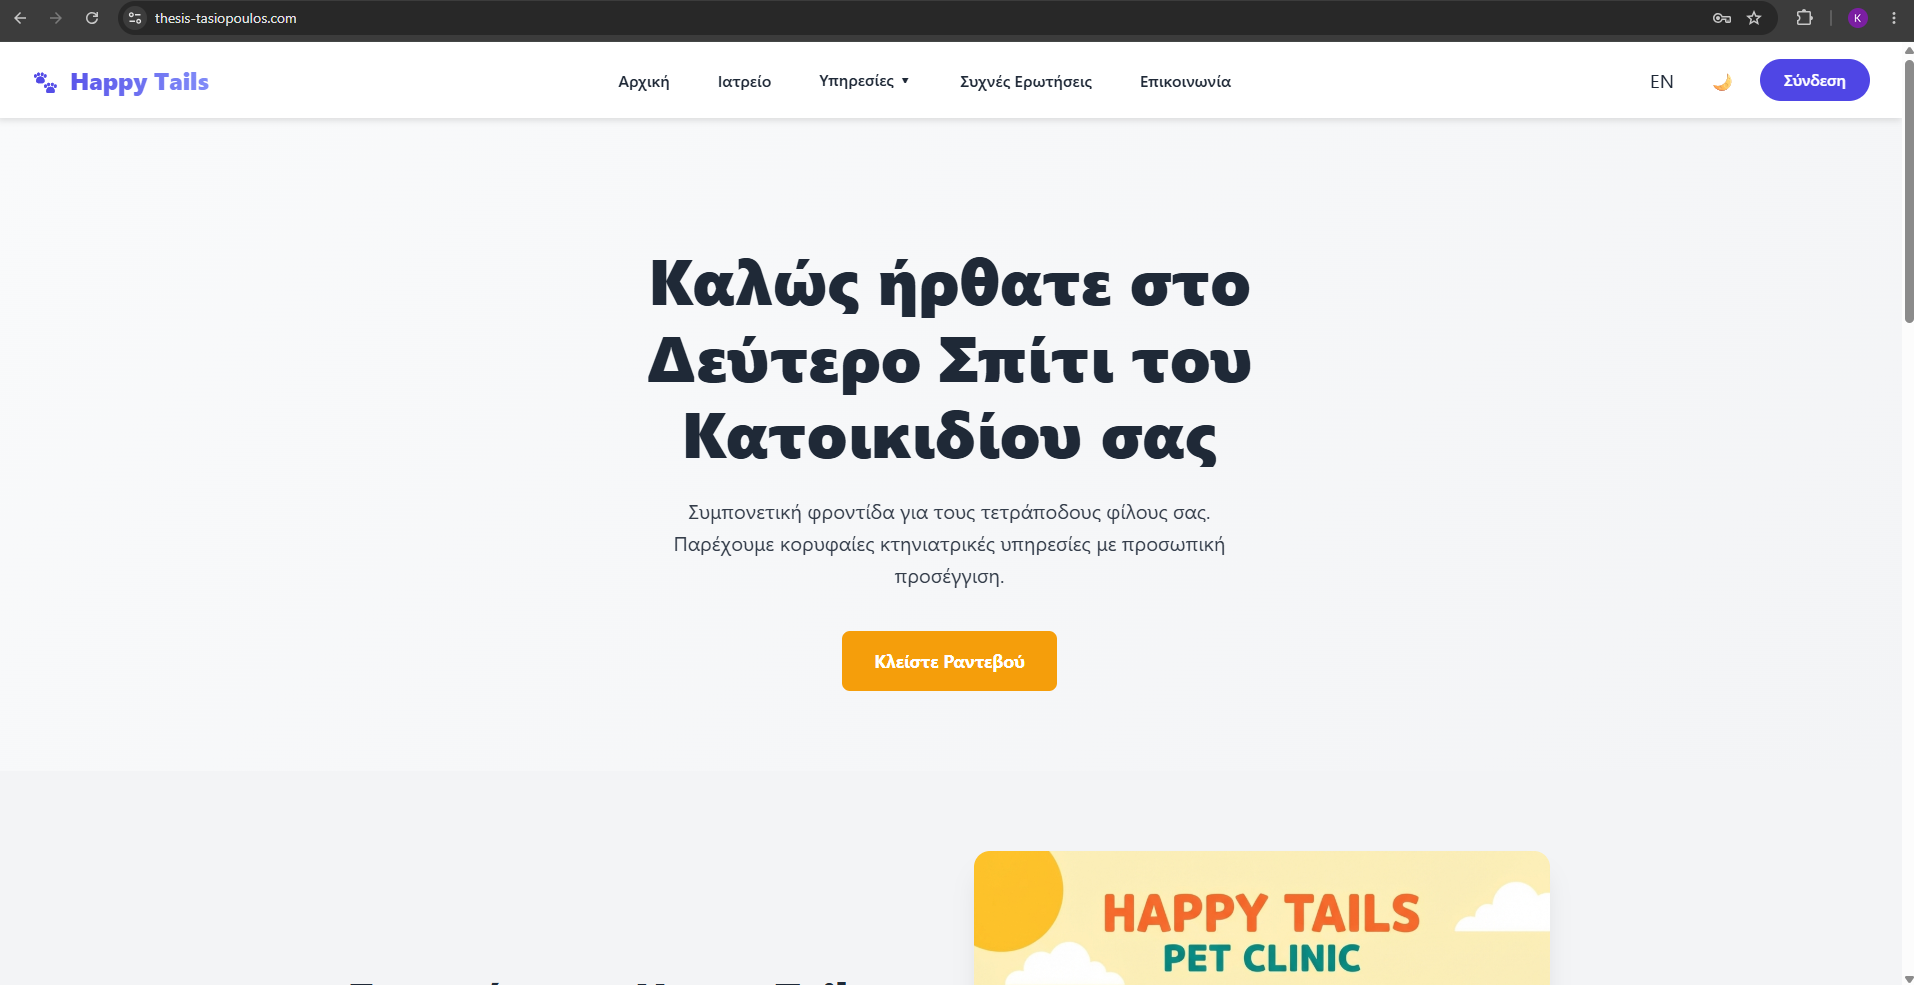
\includegraphics[width=\linewidth]{figures/application/landing-desktop.png}\\
\small (α) Desktop προβολή
\end{minipage}\hfill
\begin{minipage}[t]{0.24\textwidth}\centering
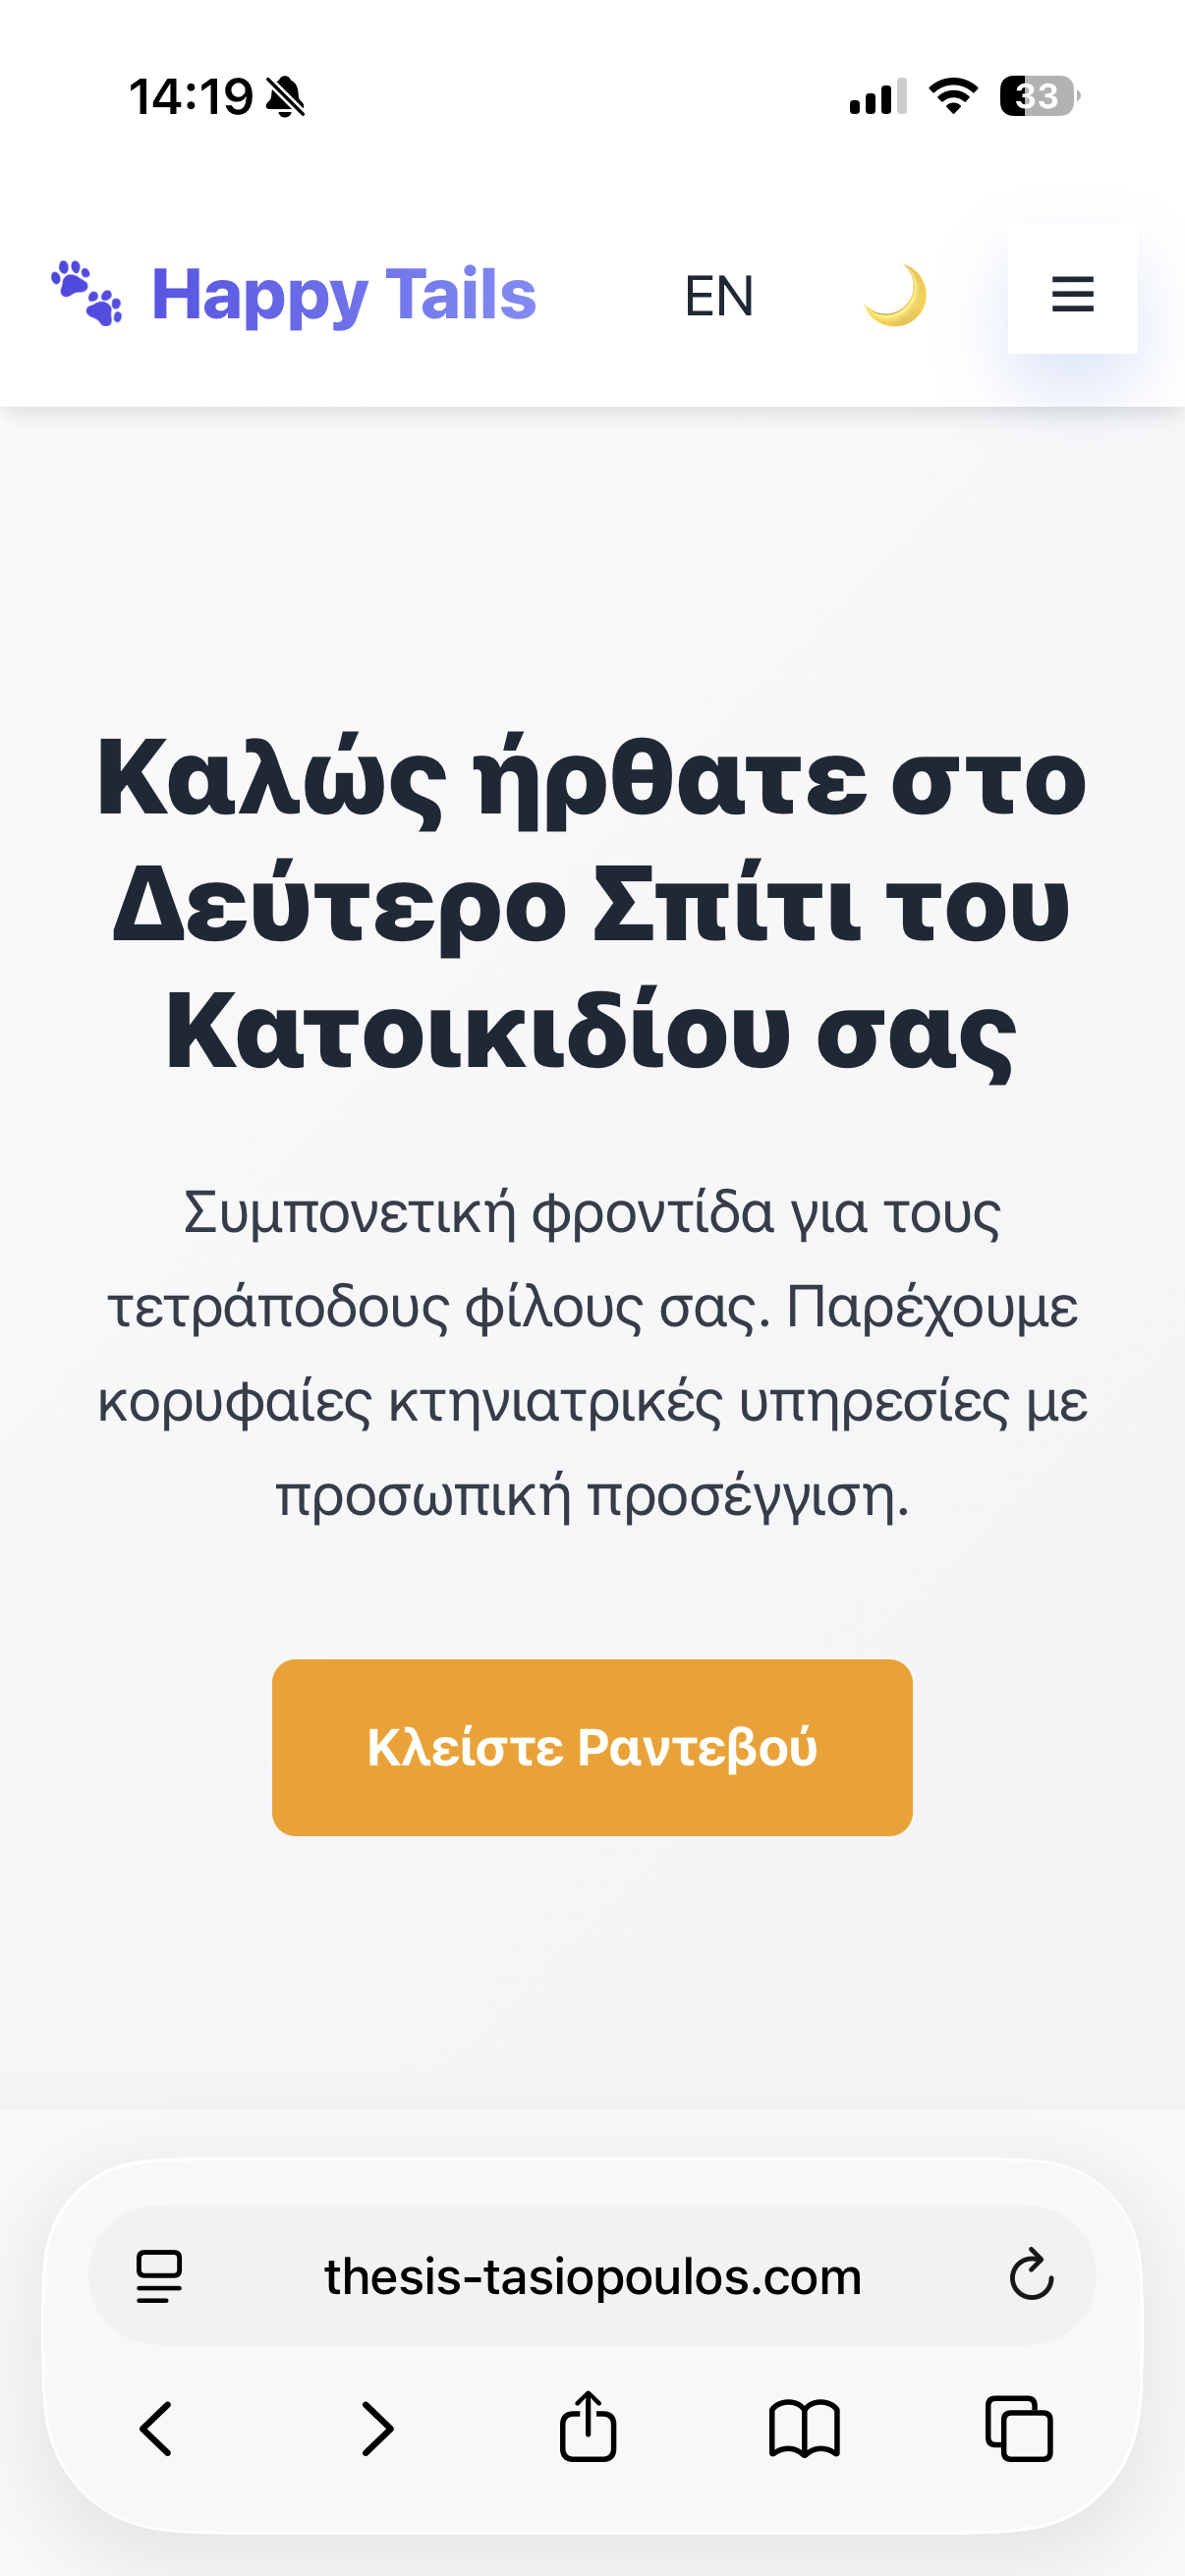
\includegraphics[width=\linewidth]{figures/application/landing-mobile.png}\\
\small (β) Mobile προβολή
\end{minipage}
\end{figure}

Η δημόσια αρχική σελίδα παρουσιάζει τον σκοπό της εφαρμογής και οδηγεί στη
σύνδεση ή στη φόρμα επικοινωνίας. Η mobile εικόνα δείχνει ότι η κεφαλίδα
συμπτύσσεται σε menu, ενώ η βασική ενέργεια παραμένει άμεσα διαθέσιμη. Στην
ενότητα της διπλωματικής παρουσιάζονται τα στοιχεία του έργου και
ενσωματωμένος χάρτης της πανεπιστημιακής τοποθεσίας. Ο χάρτης υλοποιείται με
responsive iframe και Google Maps place query, χωρίς application API key. Η
λύση είναι απλή για δημόσια πληροφορία τοποθεσίας, αλλά εξαρτά την απεικόνιση
από εξωτερικό πάροχο.

\begin{figure}[htbp]
\caption{Δημόσια ενότητα στοιχείων της διπλωματικής και ενσωματωμένος χάρτης
της πανεπιστημιακής τοποθεσίας.}
\label{fig:public-thesis-map}
\centering
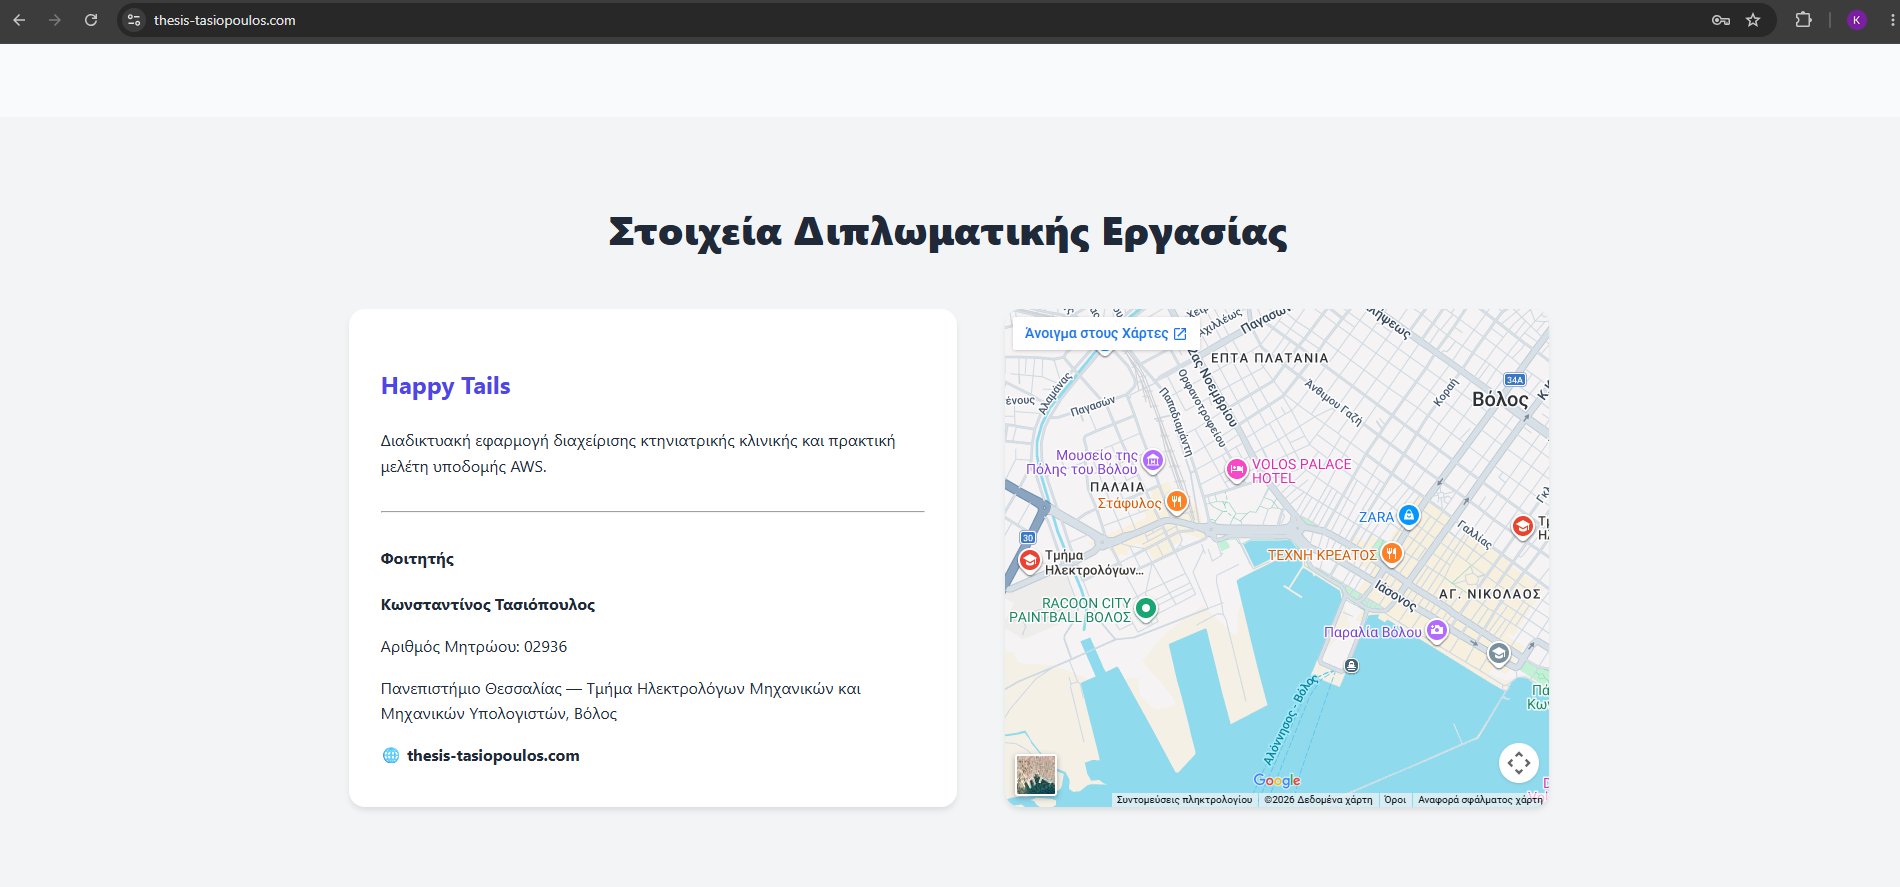
\includegraphics[width=0.9\textwidth]{figures/application/thesis-map-desktop.png}
\end{figure}

Μετά τη σύνδεση, ο πίνακας ελέγχου λειτουργεί ως σημείο προσανατολισμού. Στο
παράδειγμα εμφανίζεται ένα προσεχές ραντεβού για τη Λούνα και συνολικό πλήθος
ενός ραντεβού στην εβδομάδα. Τα δεδομένα δεν είναι στατικά στοιχεία της
σελίδας: προέρχονται από το \texttt{/api/dashboard} και υπολογίζονται από τις
αποθηκευμένες εγγραφές. Η mobile προβολή κρατά πρώτα τη σύνοψη και παρέχει
μόνιμη κάτω πλοήγηση, χρήσιμη όταν ο χρήστης χειρίζεται την εφαρμογή με το
ένα χέρι.

\begin{figure}[htbp]
\caption{Επιχειρησιακός πίνακας ελέγχου με πραγματική εγγραφή ραντεβού και
η αντίστοιχη responsive διάταξη.}
\label{fig:dashboard-responsive}
\centering
\begin{minipage}[t]{0.67\textwidth}\centering
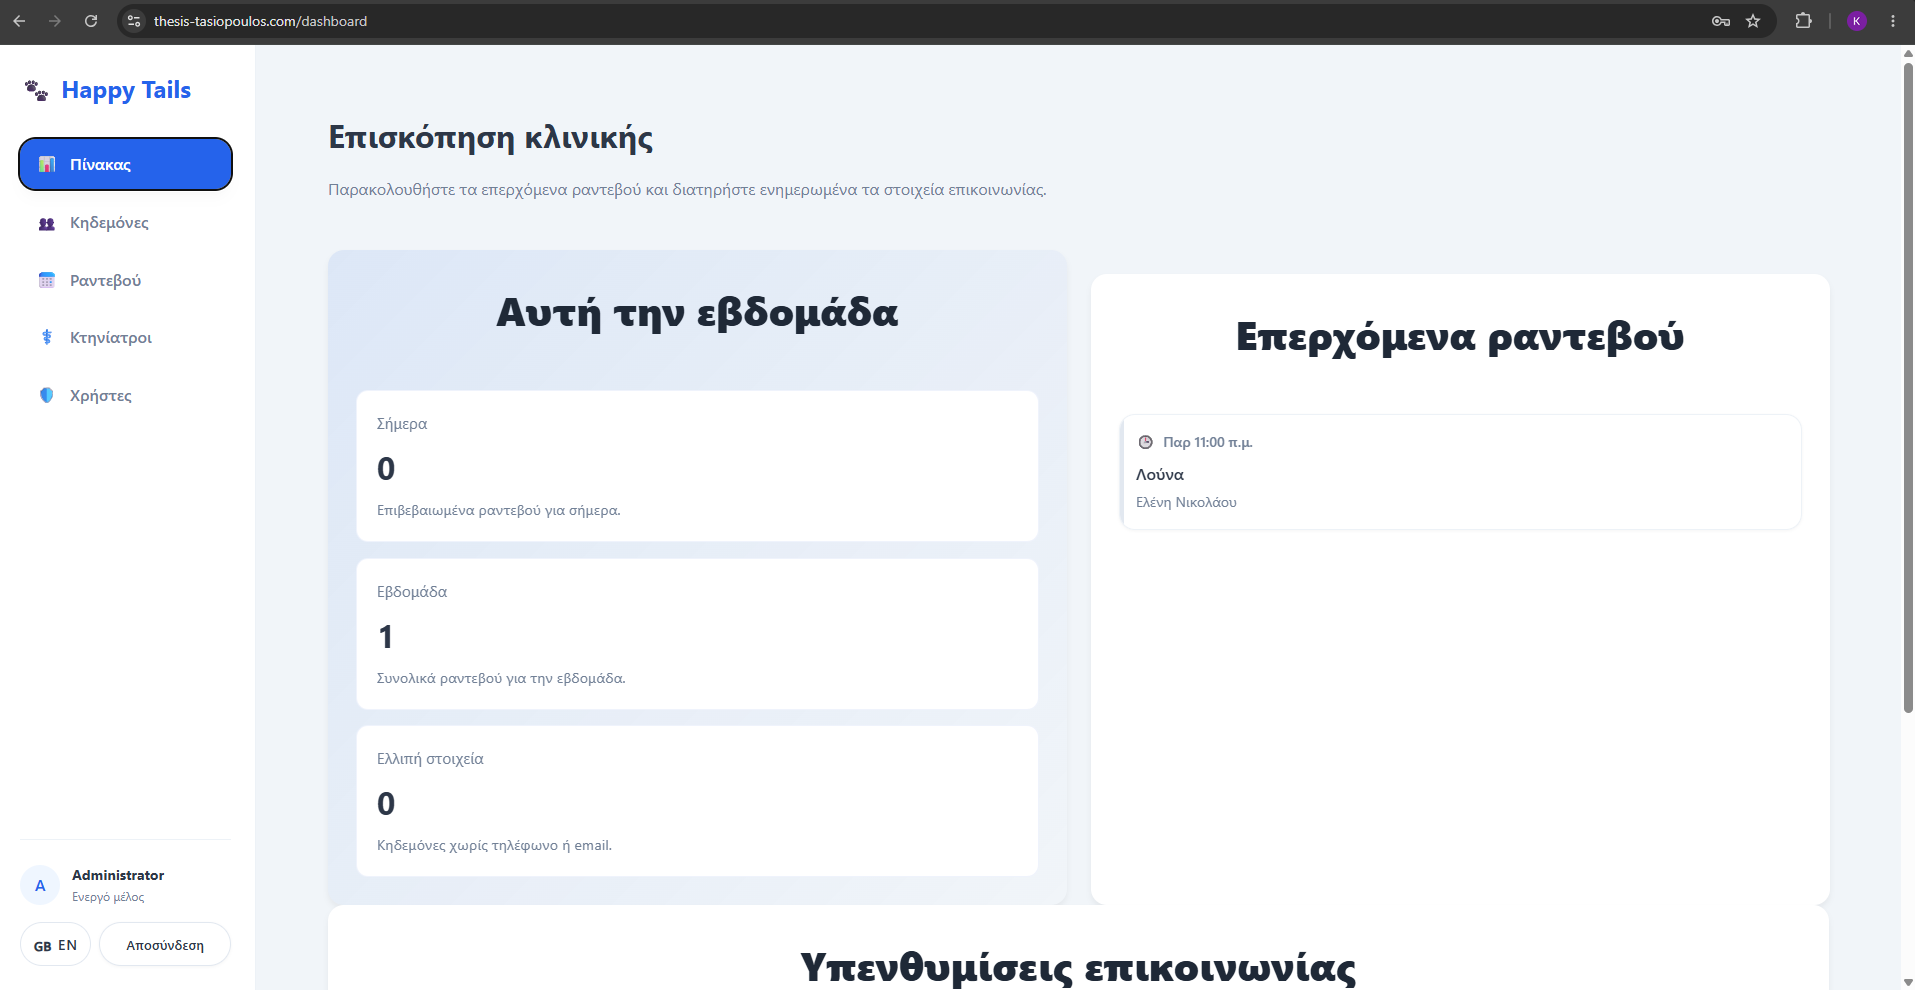
\includegraphics[width=\linewidth]{figures/application/dashboard-desktop.png}\\
\small (α) Σύνοψη σε desktop
\end{minipage}\hfill
\begin{minipage}[t]{0.24\textwidth}\centering
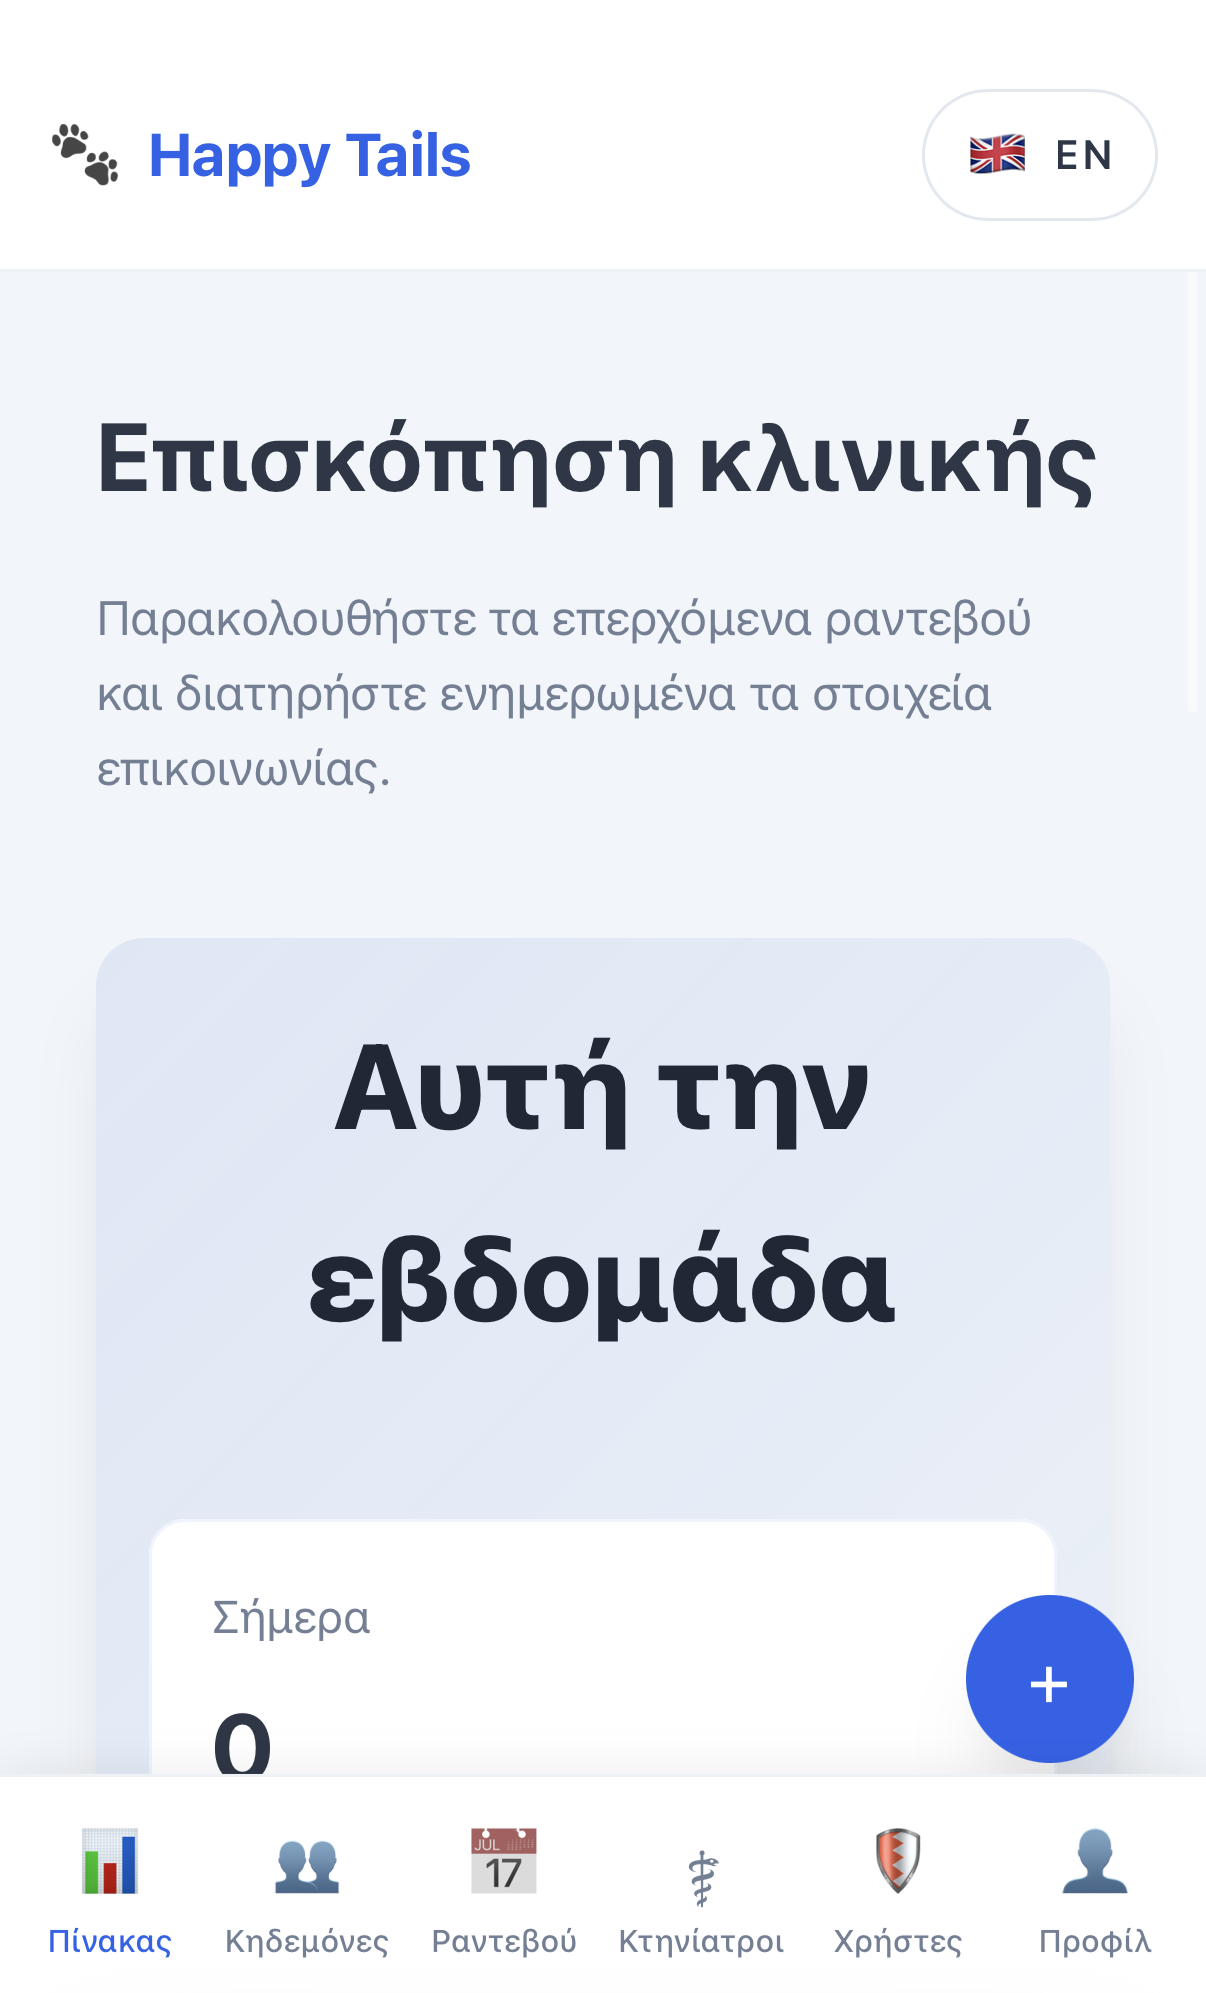
\includegraphics[width=\linewidth]{figures/application/dashboard-mobile.png}\\
\small (β) Σύνοψη σε κινητό
\end{minipage}
\end{figure}

\subsection{Καταχώριση ιδιοκτήτη και κατοικίδιου}

Η δημιουργία ιδιοκτήτη προηγείται της δημιουργίας κατοικίδιου, επειδή η
σχέση ιδιοκτησίας αποτελεί υποχρεωτικό μέρος του μοντέλου. Η φόρμα
ιδιοκτήτη αποστέλλει JSON στο \texttt{POST /api/owners}. Μετά την επιτυχή
απάντηση, ο χρήστης μεταφέρεται στην αναλυτική σελίδα και μπορεί να προσθέσει
το κατοικίδιο με \texttt{POST }\path{/api/owners/\{ownerId\}/pets}. Το frontend
ανανεώνει το query του ιδιοκτήτη και η νέα κάρτα εμφανίζεται χωρίς πλήρη
επαναφόρτωση της σελίδας.

Η Εικόνα~\ref{fig:owner-pet-responsive} παρουσιάζει το αποτέλεσμα της ροής.
Τα στοιχεία επικοινωνίας βρίσκονται μία φορά στο επίπεδο του ιδιοκτήτη, ενώ
οι γρήγορες ενέργειες του ζώου οδηγούν σε επίσκεψη, βάρος, εμβόλιο ή
απεικόνιση. Στο κινητό τα κουμπιά αναδιπλώνονται σε πλέγμα και η κάρτα
παραμένει ευανάγνωστη και οι βασικές ενέργειες είναι άμεσα διαθέσιμες χωρίς
οριζόντια μετατόπιση του κύριου περιεχομένου.

\begin{figure}[htbp]
\caption{Ολοκληρωμένη εγγραφή ιδιοκτήτη και κατοικίδιου σε desktop και
κινητό, με τις διαθέσιμες κλινικές ενέργειες.}
\label{fig:owner-pet-responsive}
\centering
\begin{minipage}[t]{0.67\textwidth}\centering
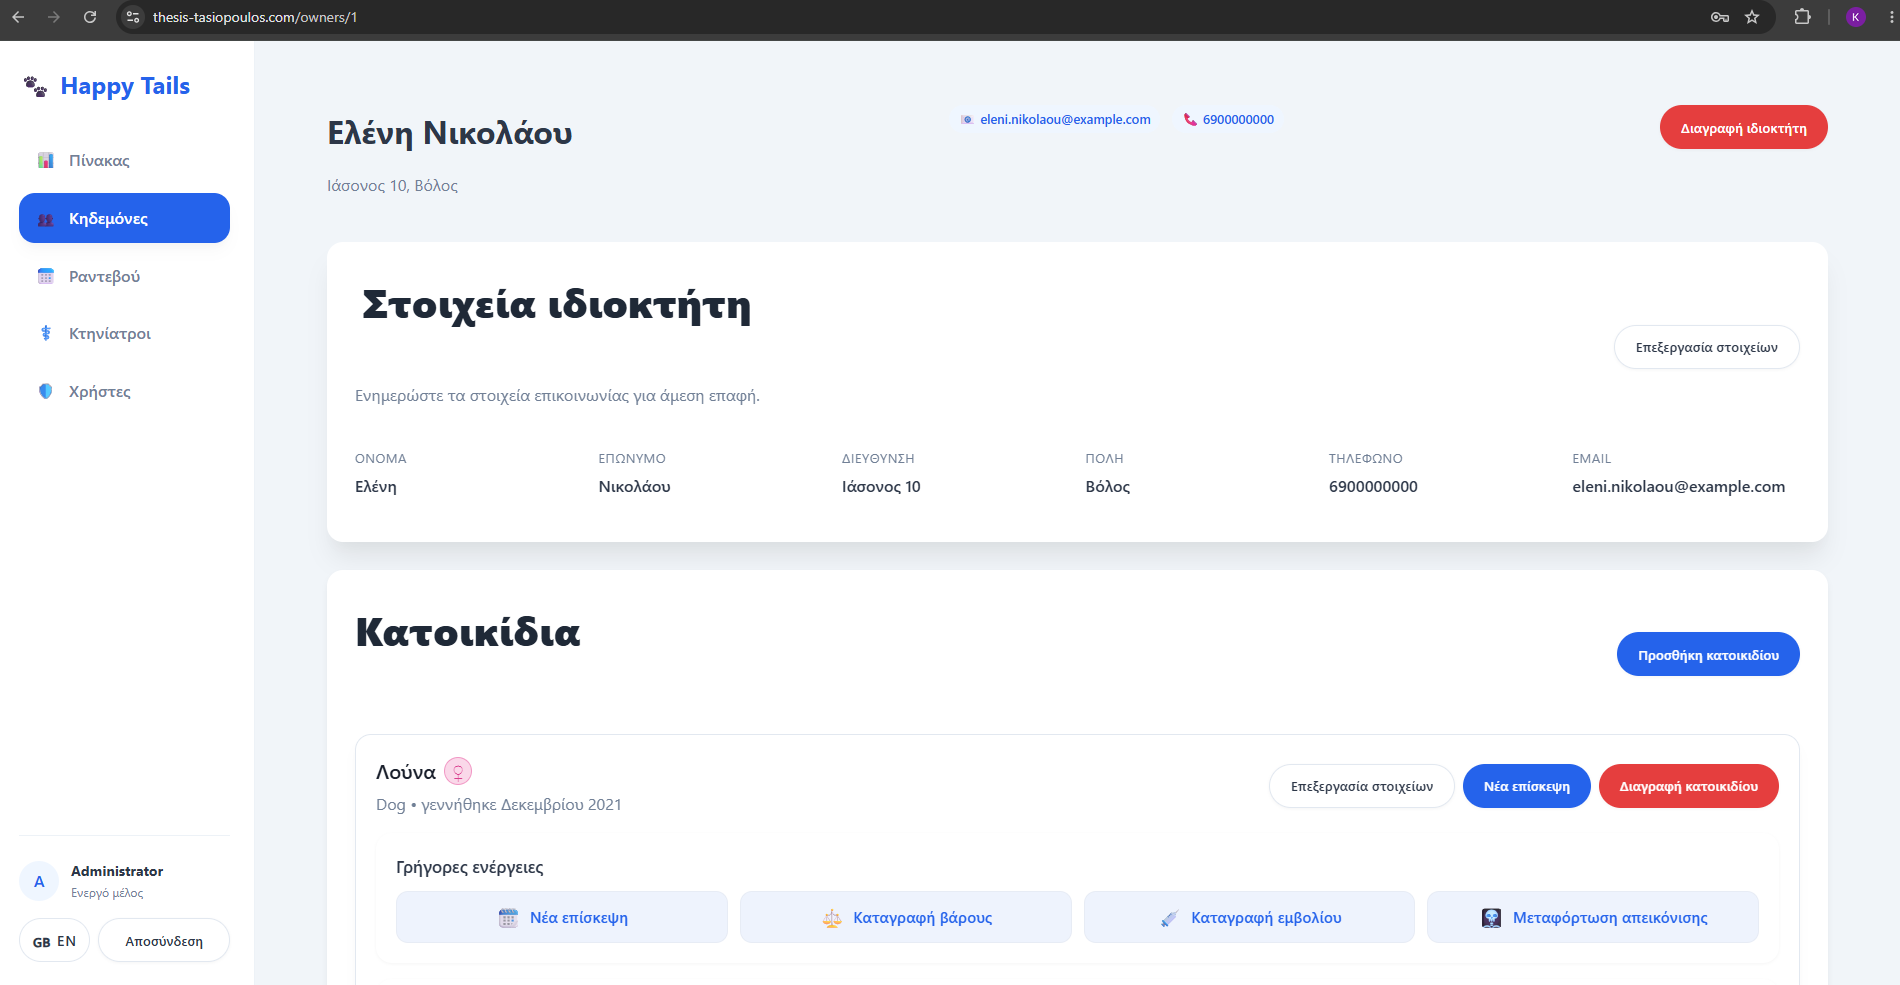
\includegraphics[width=\linewidth]{figures/application/owner-pet-desktop.png}\\
\small (α) Αναλυτική σελίδα ιδιοκτήτη
\end{minipage}\hfill
\begin{minipage}[t]{0.24\textwidth}\centering
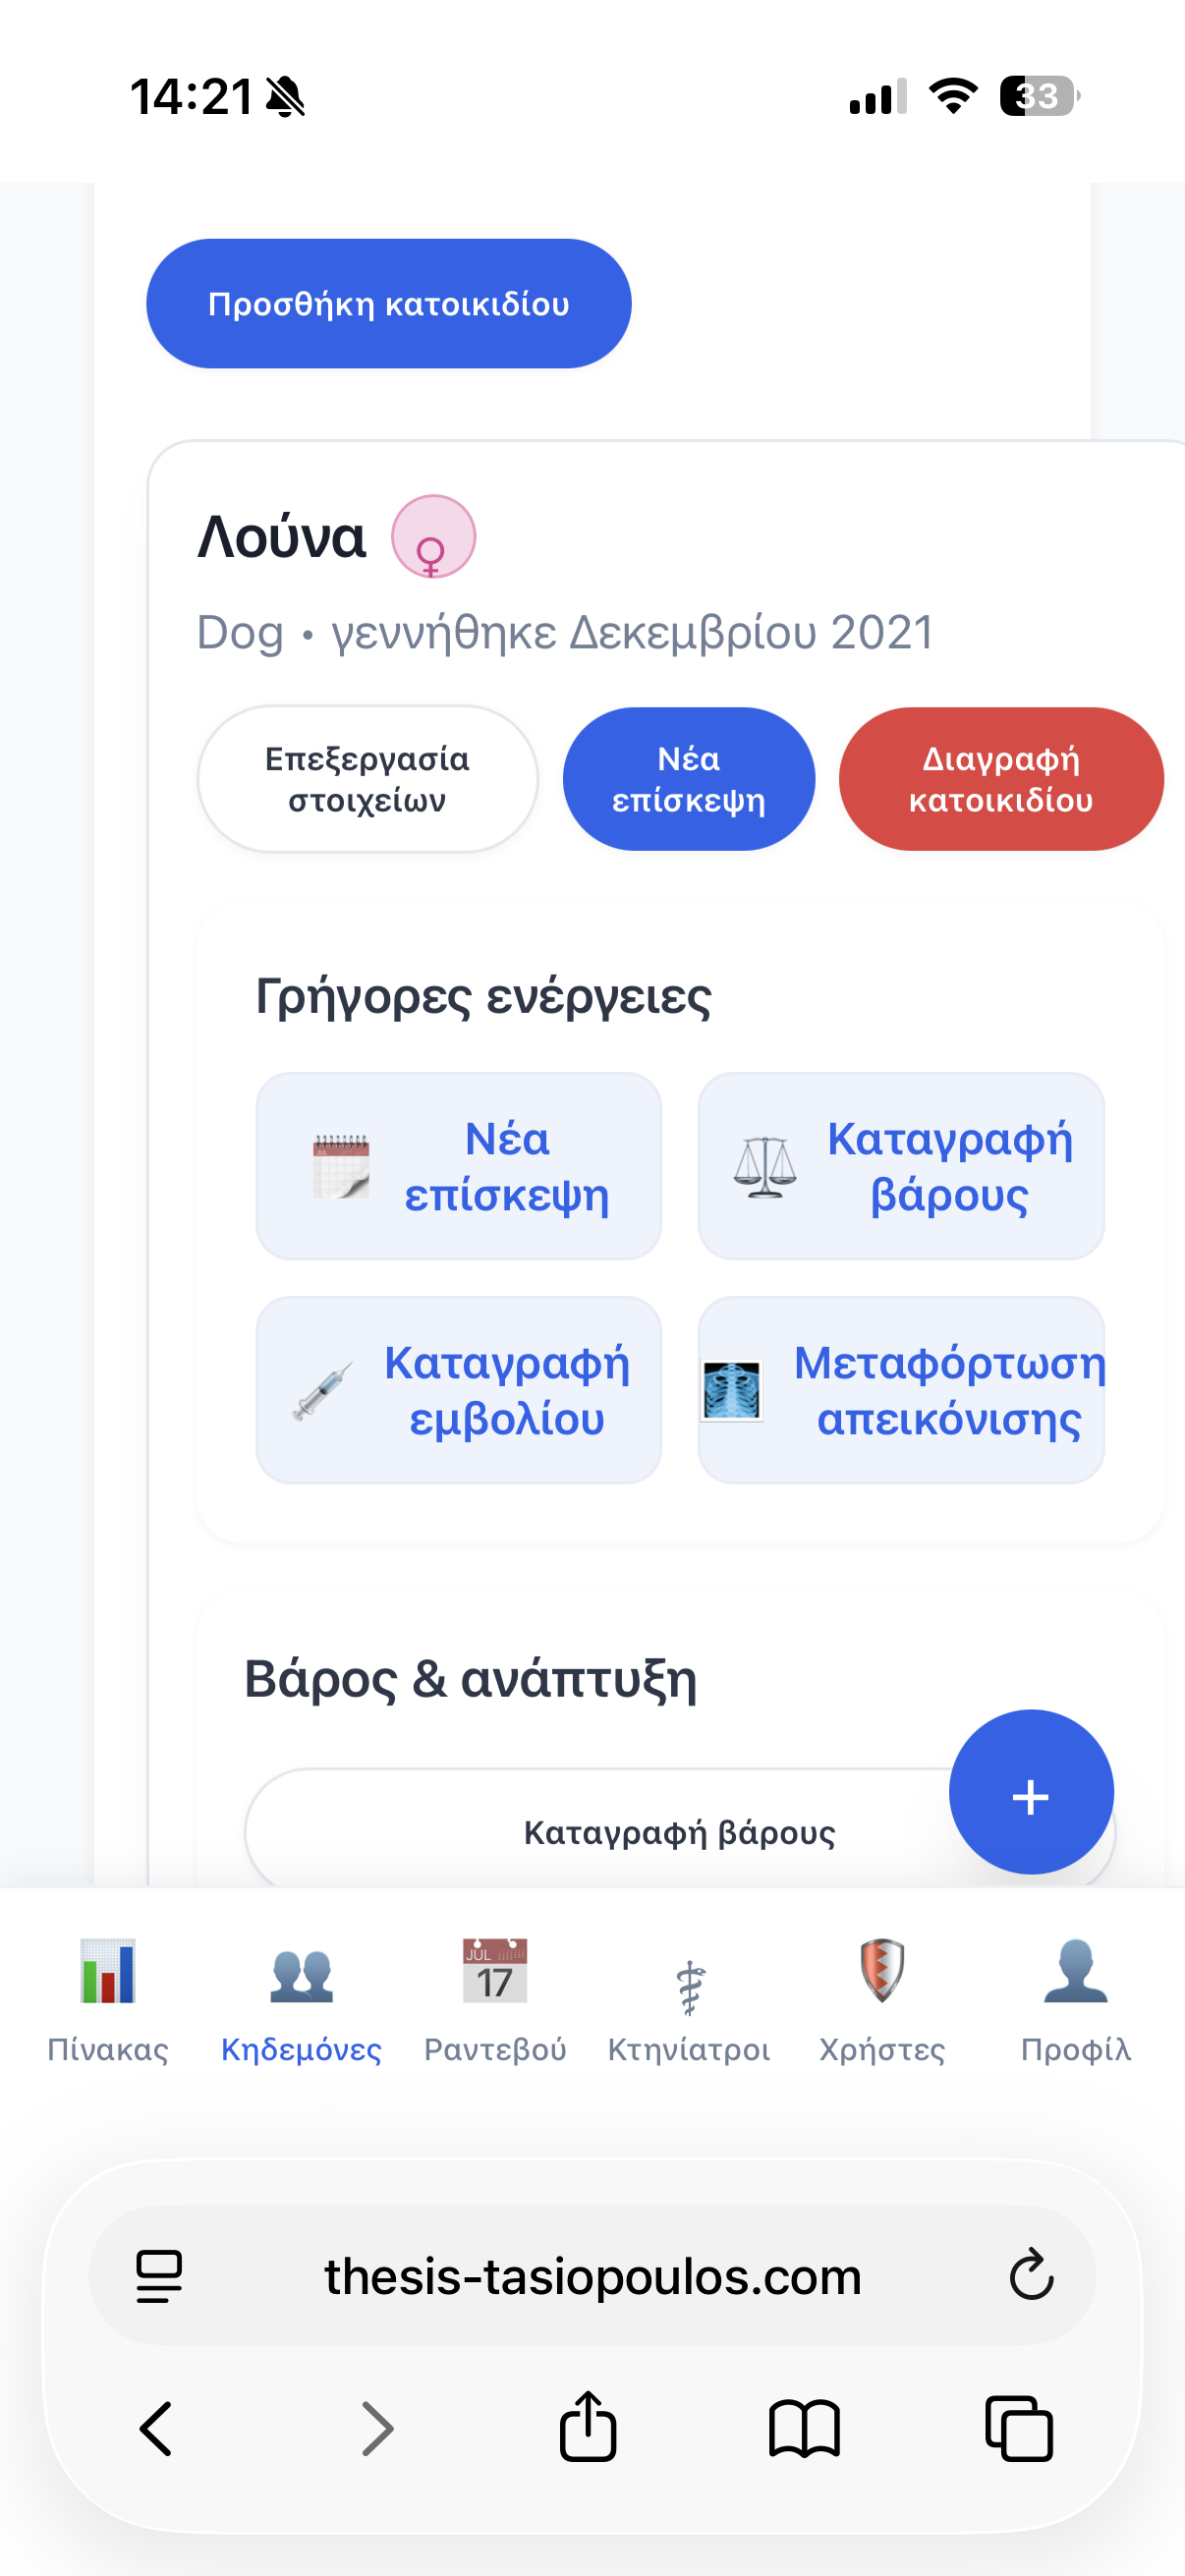
\includegraphics[width=\linewidth]{figures/application/owner-pet-mobile.png}\\
\small (β) Προσαρμογή των ενεργειών σε κινητό
\end{minipage}
\end{figure}

\subsection{Προγραμματισμός και διαχείριση ραντεβού}

Το εβδομαδιαίο ημερολόγιο συγκεντρώνει τα ραντεβού και επιτρέπει εναλλαγή
μήνα, εβδομάδας και ημέρας. Η επιλογή χρονικής θέσης ανοίγει φόρμα στην οποία
ορίζονται ιδιοκτήτης, κατοικίδιο, κτηνίατρος, ημερομηνία, ώρα και σημειώσεις.
Η επιλογή ιδιοκτήτη περιορίζει τα διαθέσιμα κατοικίδια, αποφεύγοντας
ασυνεπείς συνδυασμούς. Μετά το save, η επιτυχία εμφανίζεται μέσα στο drawer
και το calendar query ανανεώνεται.

Στη mobile προβολή οι ημέρες δεν συρρικνώνονται όλες στο πλάτος της οθόνης.
Η σύνοψη παραμένει σε οριζόντια λωρίδα και τα πλήκτρα προηγούμενης και
επόμενης εβδομάδας μετακινούν τη χρονική περίοδο. Η συμπεριφορά είναι
σκόπιμη: προτιμάται η αναγνωσιμότητα μιας ημέρας από ένα πλήρες αλλά
δυσανάγνωστο πλέγμα επτά πολύ στενών στηλών.

\begin{figure}[htbp]
\caption{Εβδομαδιαίο πρόγραμμα και προσαρμογή της πλοήγησης ραντεβού σε
κινητή συσκευή.}
\label{fig:calendar-responsive}
\centering
\begin{minipage}[t]{0.67\textwidth}\centering
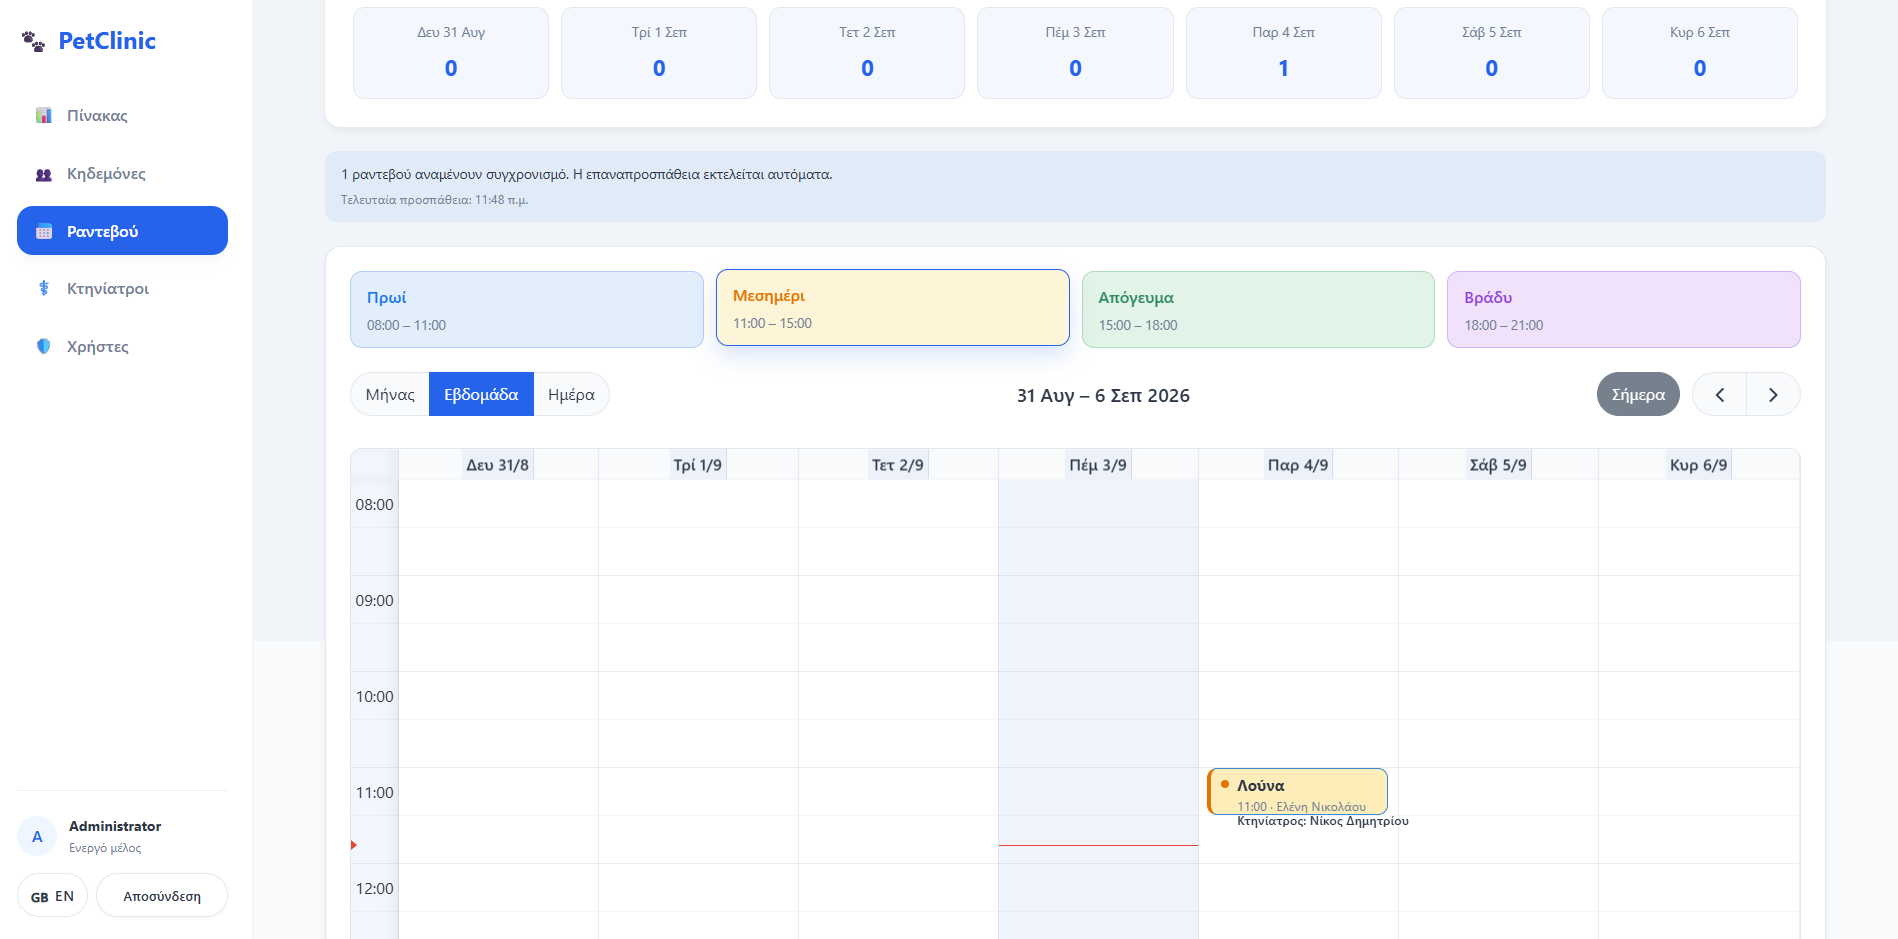
\includegraphics[width=\linewidth]{figures/application/calendar-week-desktop.png}\\
\small (α) Εβδομαδιαίο ημερολόγιο
\end{minipage}\hfill
\begin{minipage}[t]{0.24\textwidth}\centering
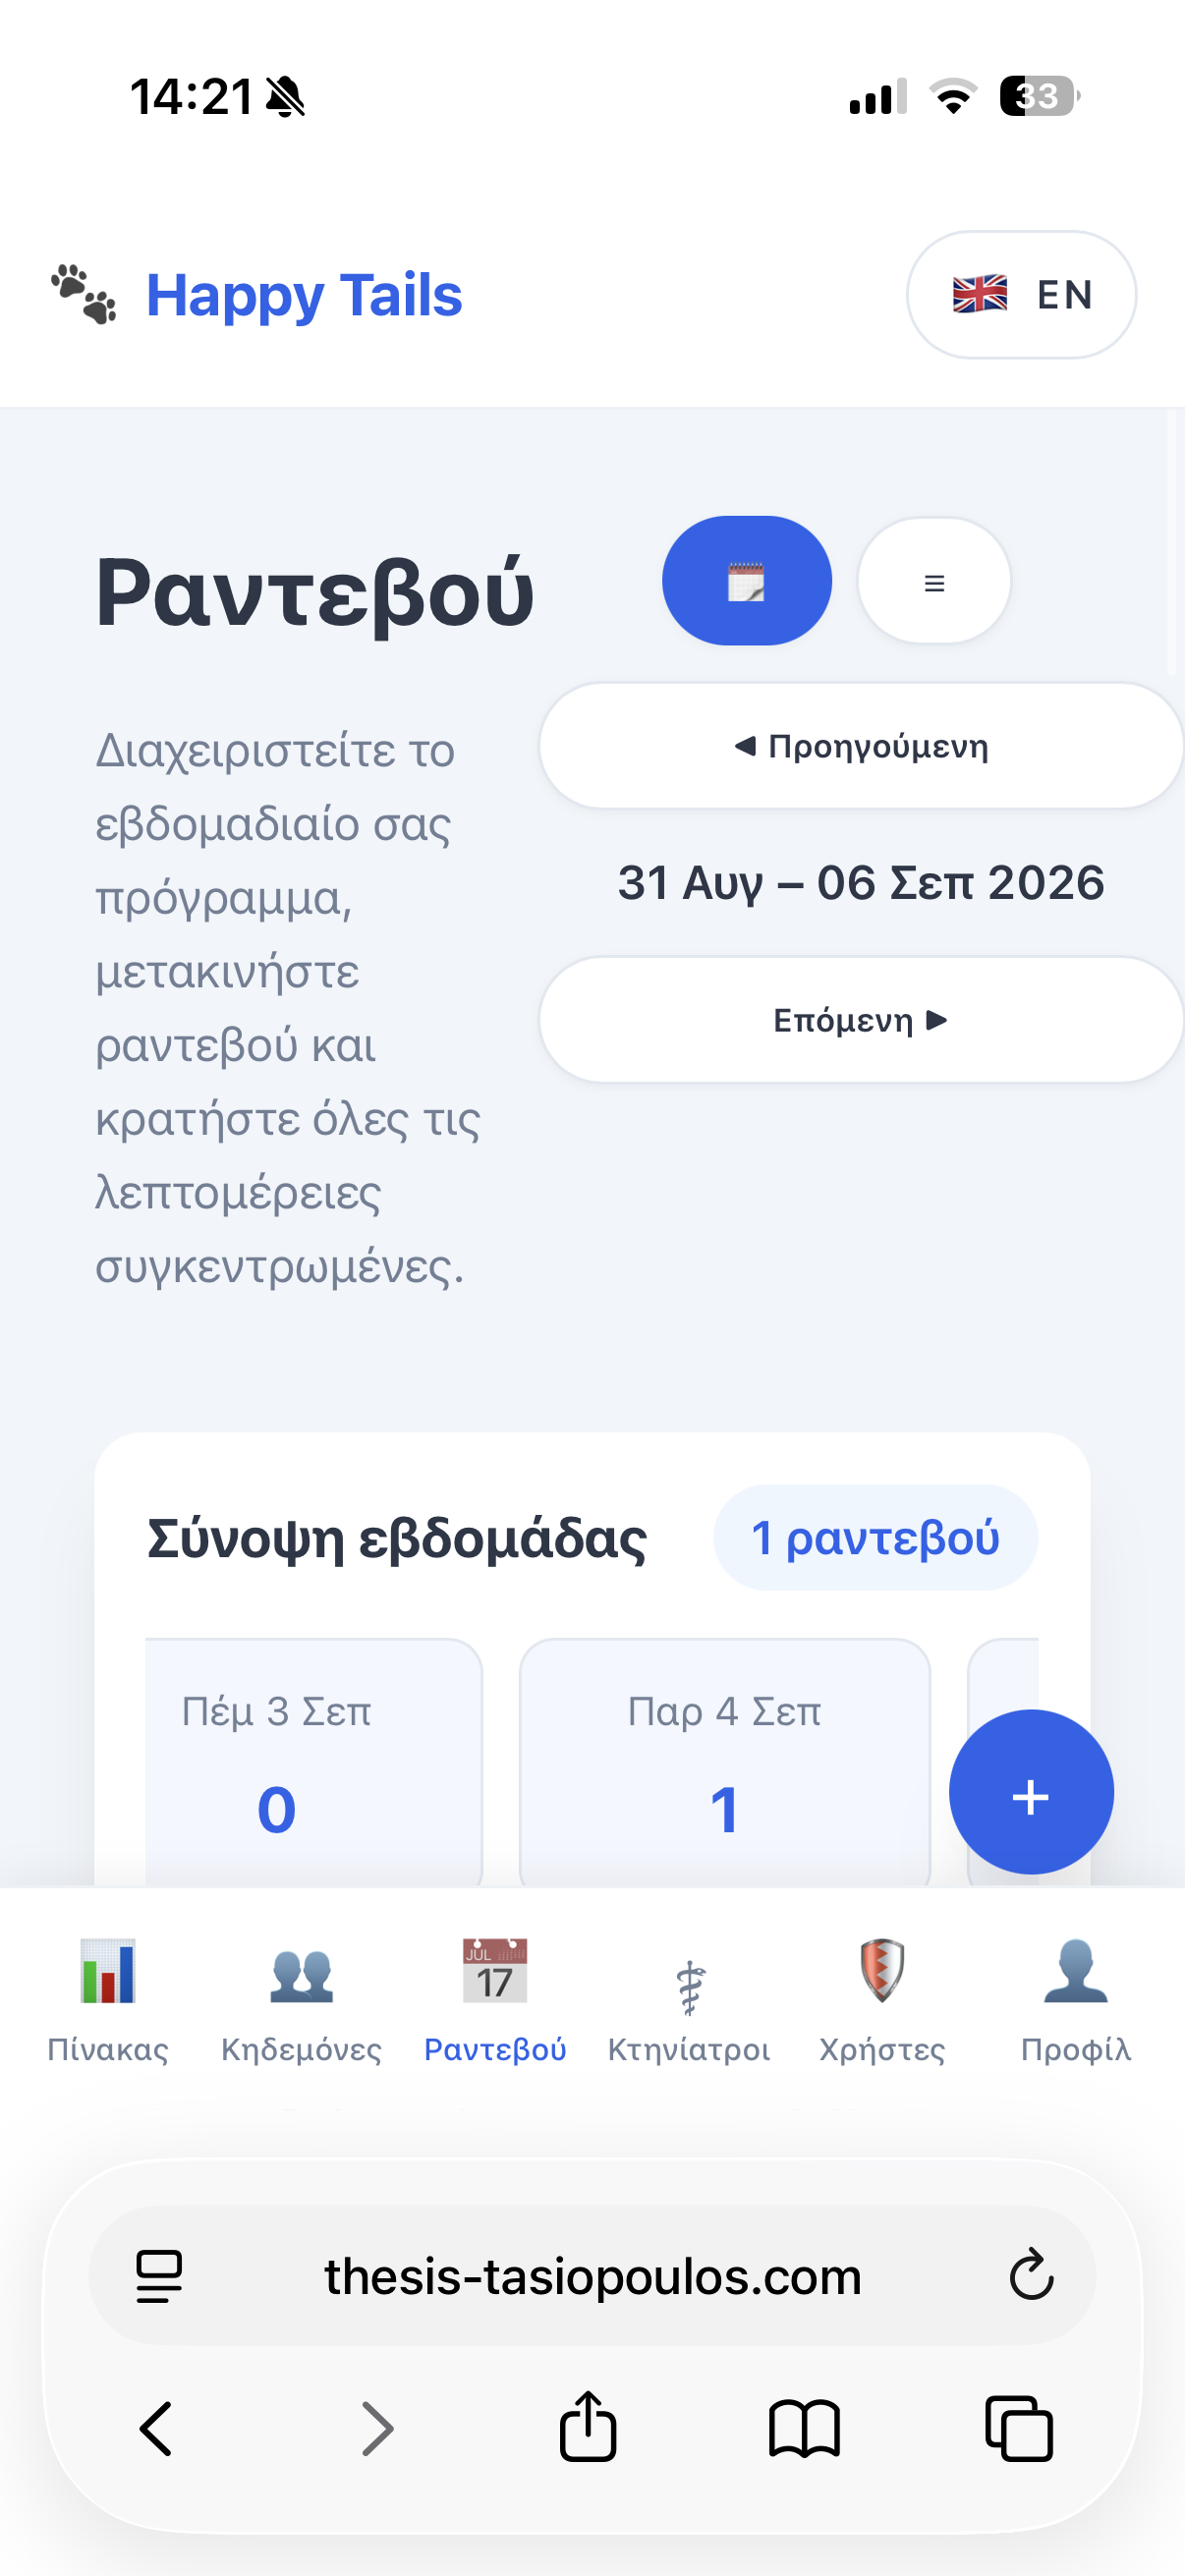
\includegraphics[width=\linewidth]{figures/application/appointments-mobile.png}\\
\small (β) Mobile σύνοψη και χρονική πλοήγηση
\end{minipage}
\end{figure}

\subsection{Διαχείριση επίσκεψης και κτηνιατρικού ιστορικού}

Η επιλογή ενός ραντεβού ανοίγει πλευρικό drawer χωρίς να χάνεται το πλαίσιο
του ημερολογίου. Ο χρήστης μπορεί να ενημερώσει τα στοιχεία της επίσκεψης
και να προσθέσει ιατρικό φάκελο. Η φόρμα φακέλου υποστηρίζει ζωτικές
μετρήσεις και αρχεία. Επειδή το περιεχόμενο είναι μεγαλύτερο από το ύψος
μιας συνηθισμένης οθόνης, το drawer διαθέτει ανεξάρτητη κατακόρυφη κύλιση και
σταθερή επικεφαλίδα. Το στιγμιότυπο μετά την αποθήκευση αποδεικνύει ότι η
μεταβολή ολοκληρώθηκε, ενώ η δεύτερη όψη δείχνει τις διαθέσιμες μετρήσεις και
την ήδη αποθηκευμένη εγγραφή.

\begin{figure}[htbp]
\caption{Αποθήκευση στοιχείων ραντεβού και καταχώριση ζωτικών μετρήσεων στον
ιατρικό φάκελο από το ίδιο πλευρικό drawer.}
\label{fig:appointment-record}
\centering
\begin{minipage}[t]{0.49\textwidth}\centering
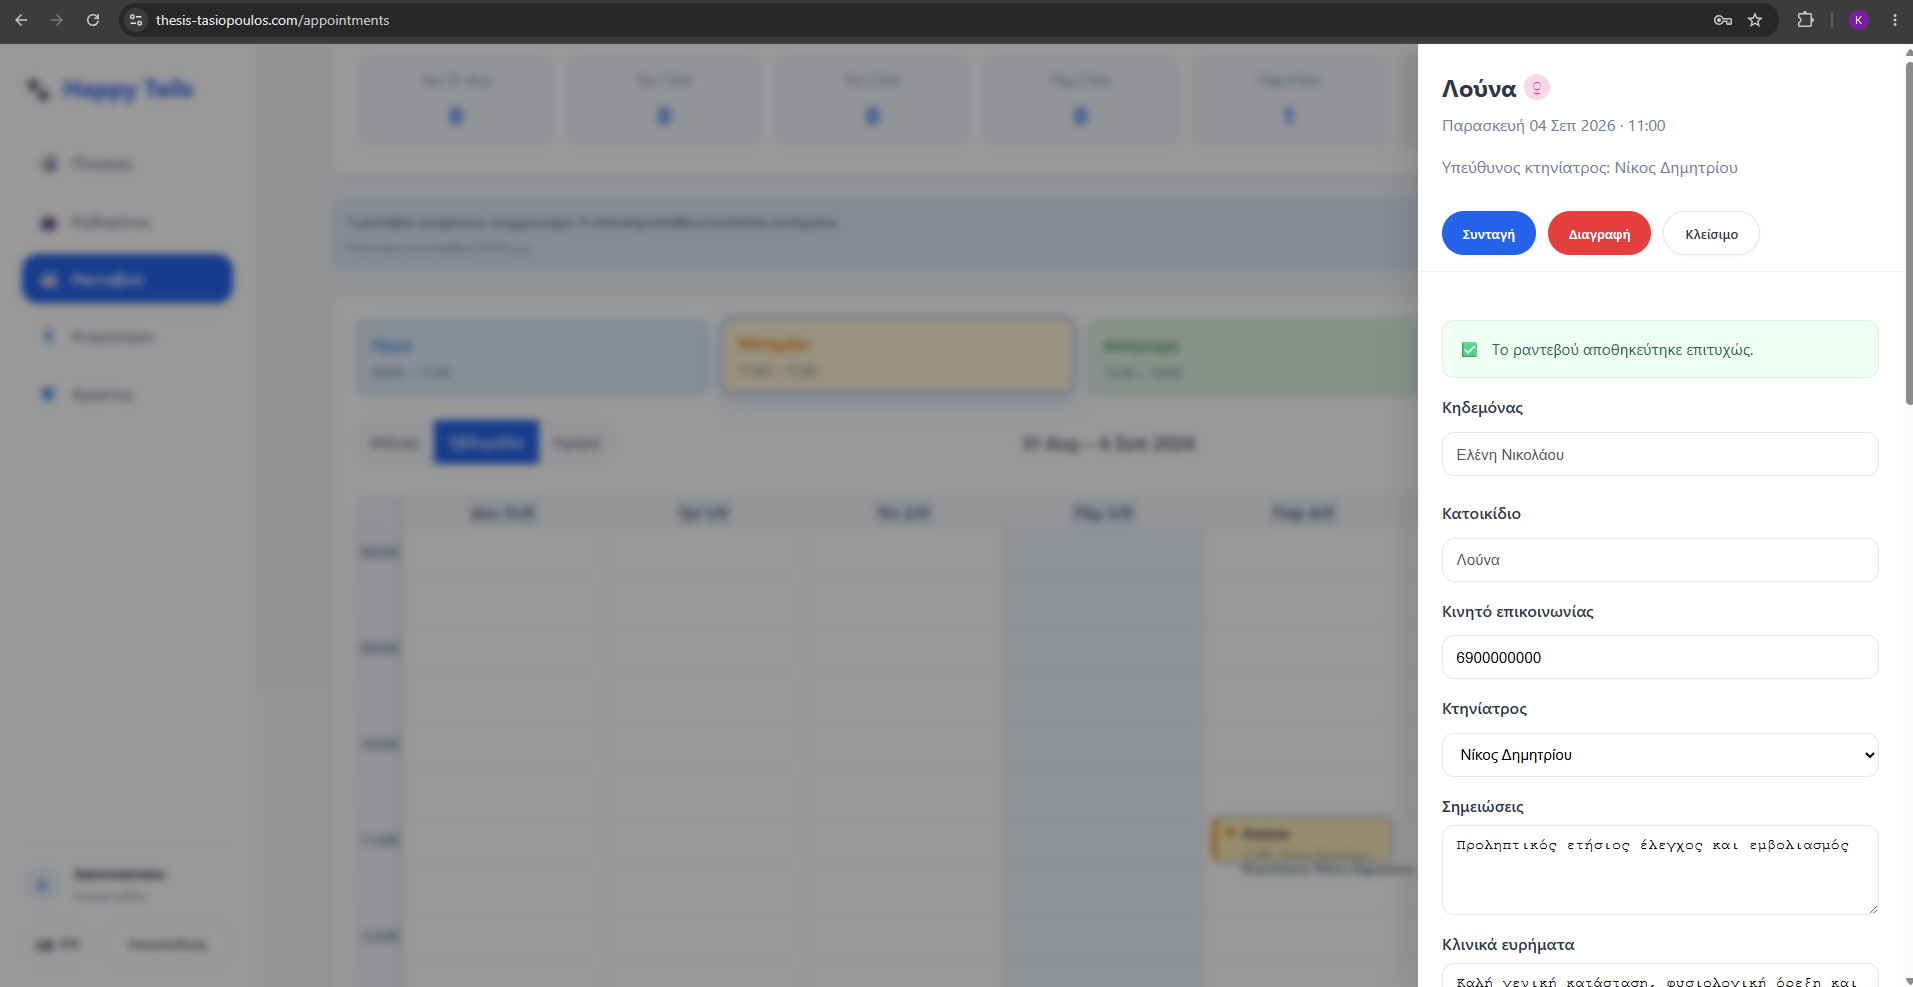
\includegraphics[width=\linewidth]{figures/application/appointment-save-desktop.png}\\
\small (α) Επιβεβαίωση επιτυχούς αποθήκευσης
\end{minipage}\hfill
\begin{minipage}[t]{0.49\textwidth}\centering
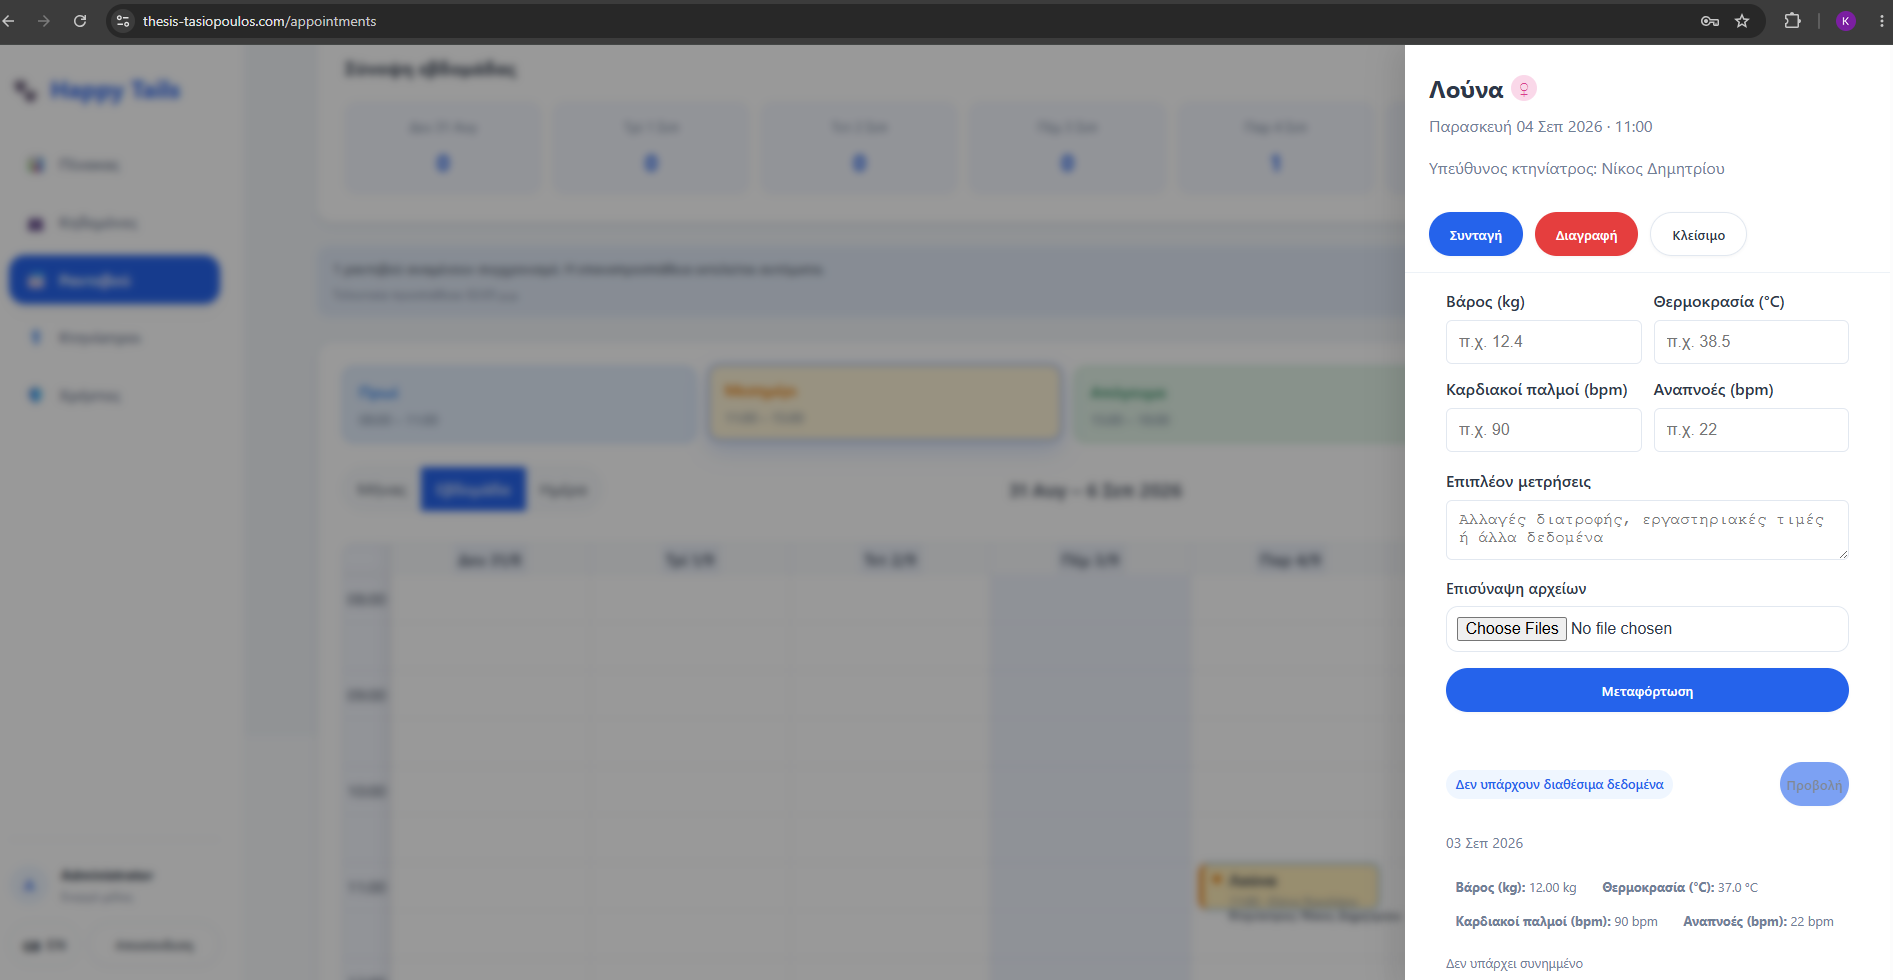
\includegraphics[width=\linewidth]{figures/application/health-record-desktop.png}\\
\small (β) Μετρήσεις και συνημμένα ιατρικού φακέλου
\end{minipage}
\end{figure}

Η καταχώριση βάρους τροφοδοτεί τη γραφική παράσταση στην καρτέλα του
κατοικίδιου. Το γράφημα δεν αποτελεί ξεχωριστή αποθήκη δεδομένων· είναι
παράγωγη απεικόνιση των health records που περιέχουν τιμή βάρους. Αντίστοιχα,
η συνταγή χρησιμοποιεί τα στοιχεία της κλινικής, του ζώου και του ιδιοκτήτη
για να δημιουργήσει εκτυπώσιμη προβολή, την οποία ο browser μπορεί να
αποθηκεύσει ως PDF. Με αυτόν τον τρόπο τα δεδομένα που καταχωρίστηκαν για την
κλινική εργασία μπορούν να εξαχθούν σε μορφή κατάλληλη για παράδοση.

\begin{figure}[htbp]
\caption{Παράγωγα της κλινικής πληροφορίας: διάγραμμα πορείας βάρους και
εκτυπώσιμη συνταγή.}
\label{fig:clinical-outputs}
\centering
\begin{minipage}[t]{0.49\textwidth}\centering
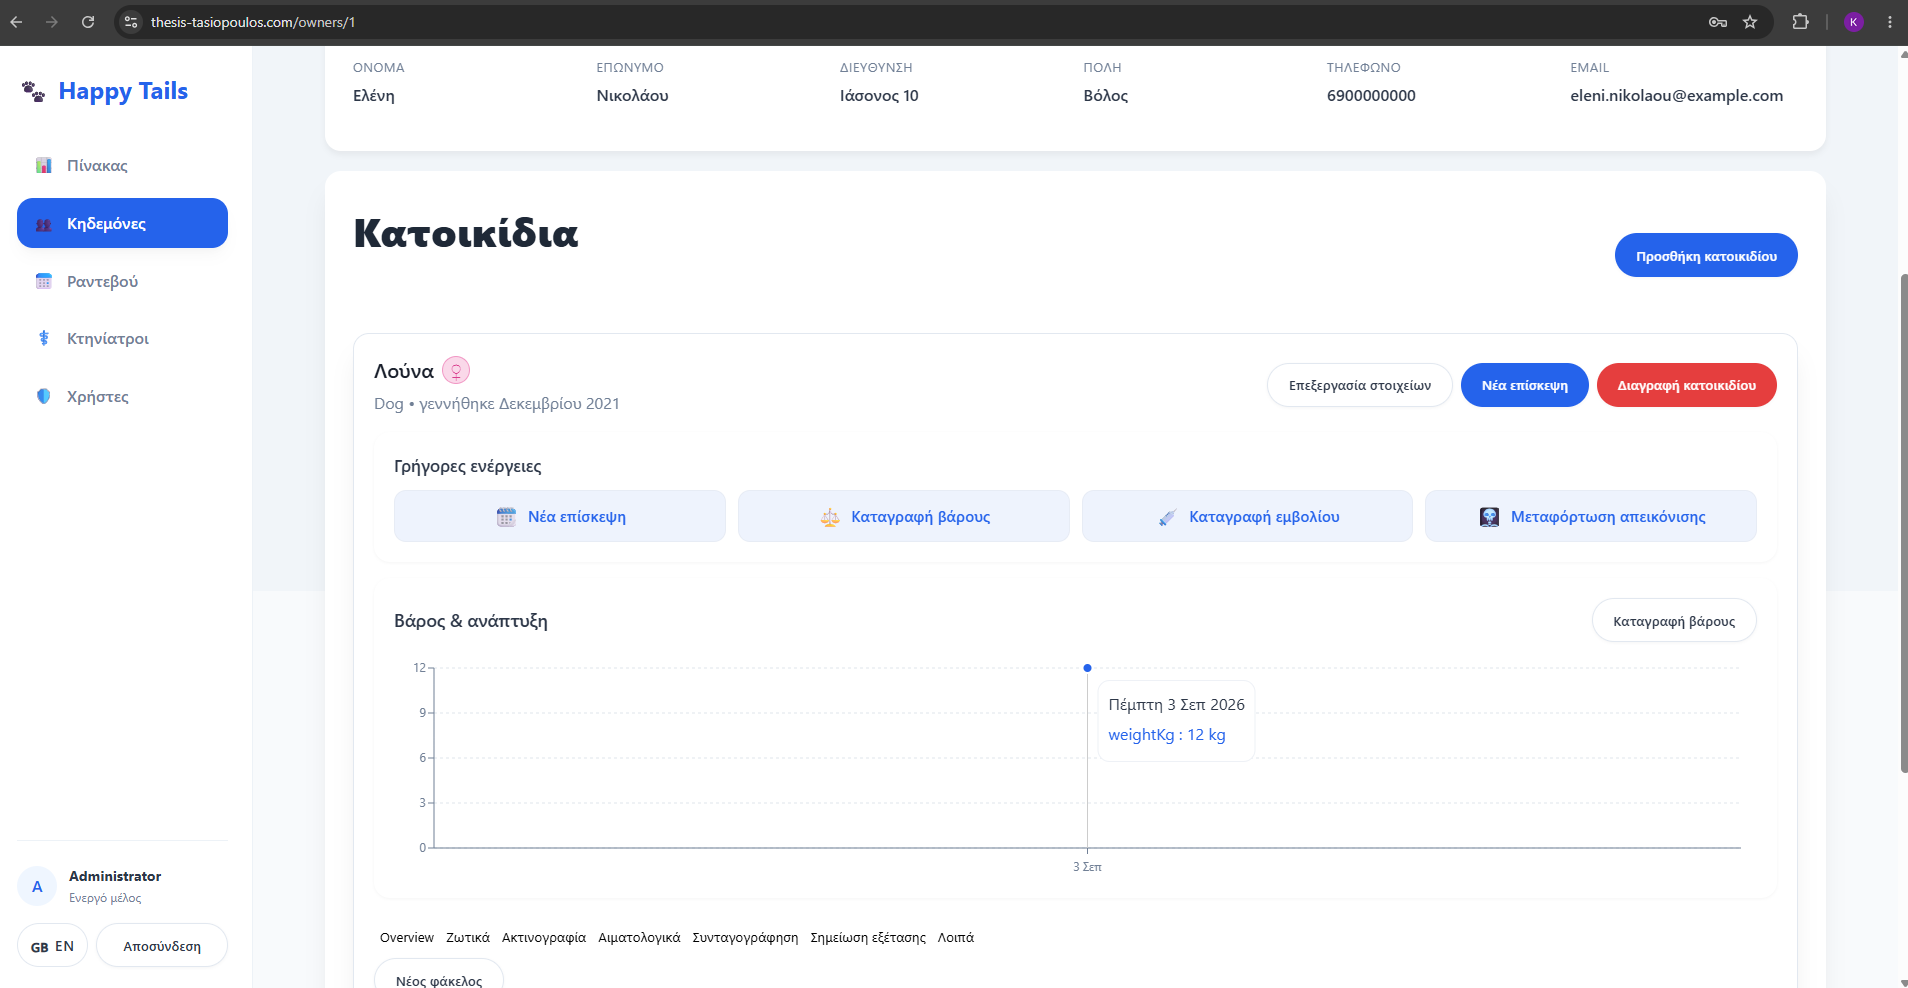
\includegraphics[width=\linewidth]{figures/application/weight-chart-desktop.png}\\
\small (α) Ιστορικό βάρους
\end{minipage}\hfill
\begin{minipage}[t]{0.49\textwidth}\centering
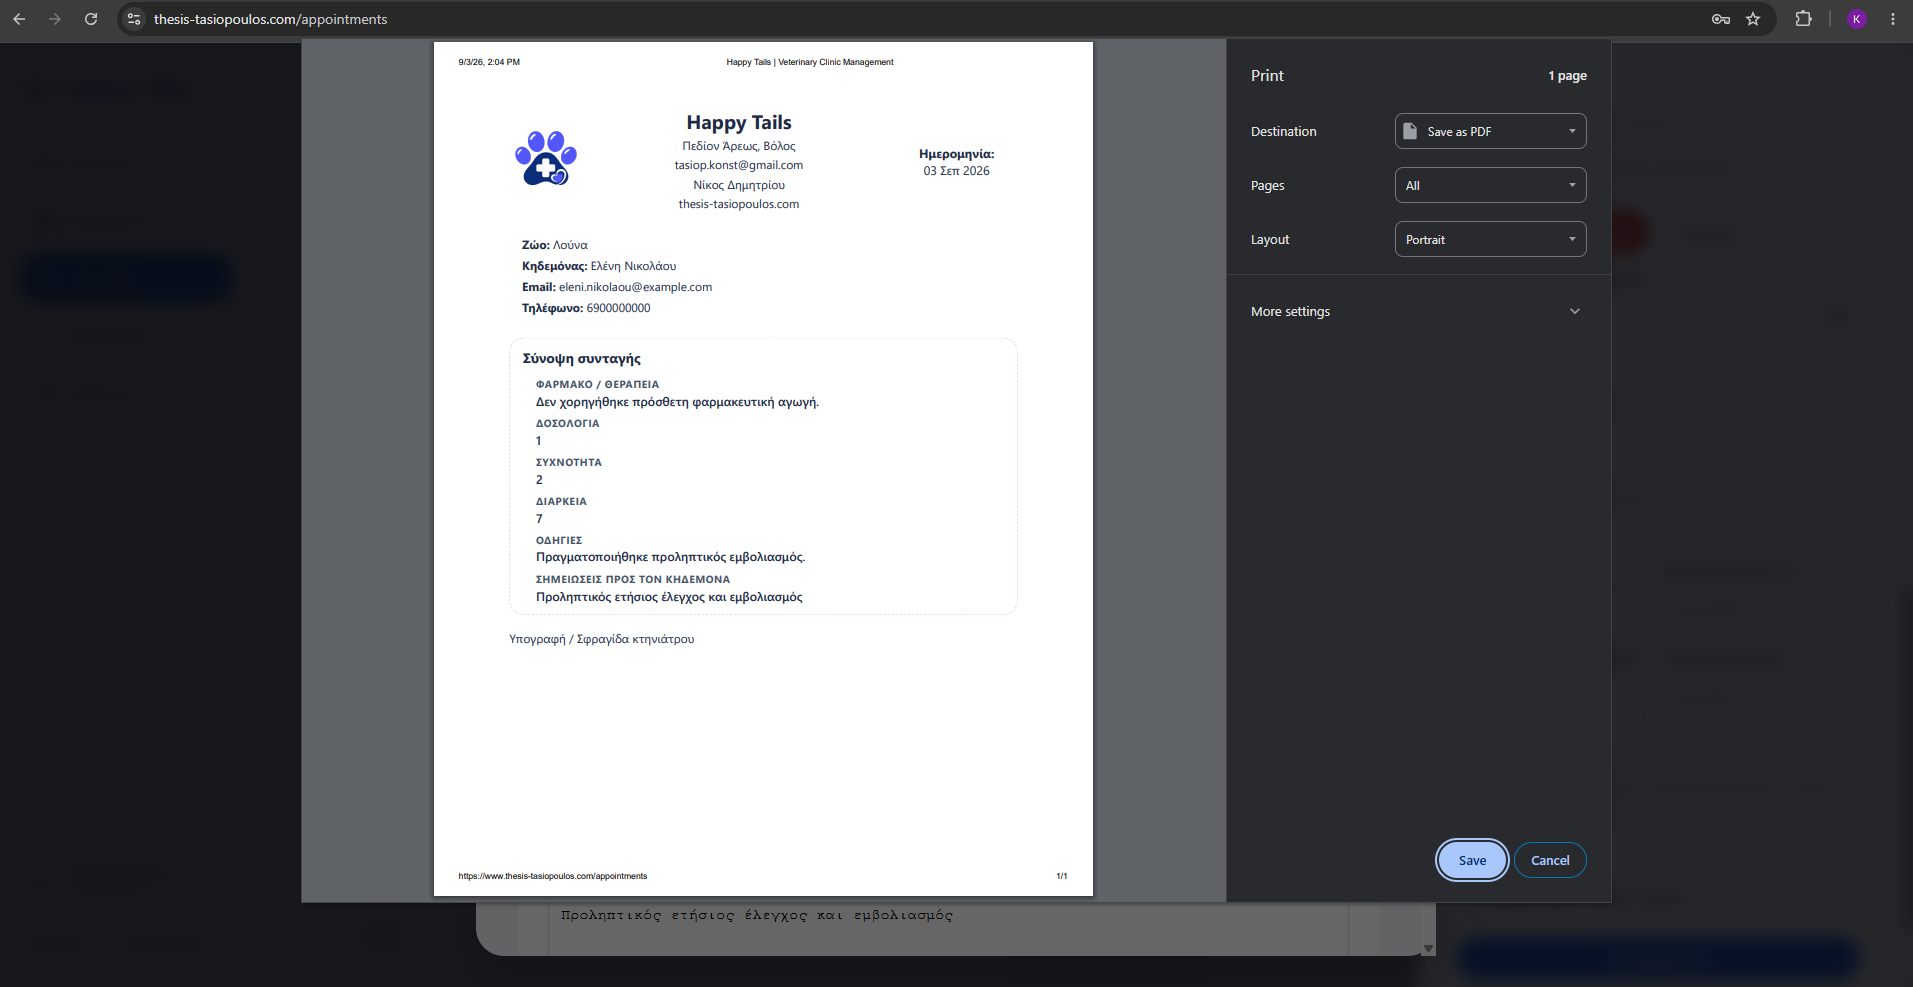
\includegraphics[width=\linewidth]{figures/application/prescription-print-desktop.png}\\
\small (β) Προεπισκόπηση εκτύπωσης συνταγής
\end{minipage}
\end{figure}

\subsection{Διοίκηση χρηστών}

Η σελίδα χρηστών διαχωρίζει εκκρεμείς, ενεργούς και αποκλεισμένους
λογαριασμούς. Από εδώ ο διαχειριστής μπορεί να εγκρίνει έναν χρήστη, να τον
απενεργοποιήσει, να τον αποκλείσει ή να ενημερώσει τους ρόλους του. Η
διεύθυνση email εμφανίζεται ώστε η απόφαση να συνδέεται με συγκεκριμένη
αίτηση. Στην Εικόνα~\ref{fig:admin-users} ο ενεργός λογαριασμός της
εγκατάστασης εμφανίζεται με τη διεύθυνση επικοινωνίας που έχει οριστεί στην
production παραμετροποίηση.

\begin{figure}[htbp]
\caption{Διοικητική προβολή ενεργών χρηστών και ενεργειών ελέγχου πρόσβασης.}
\label{fig:admin-users}
\centering
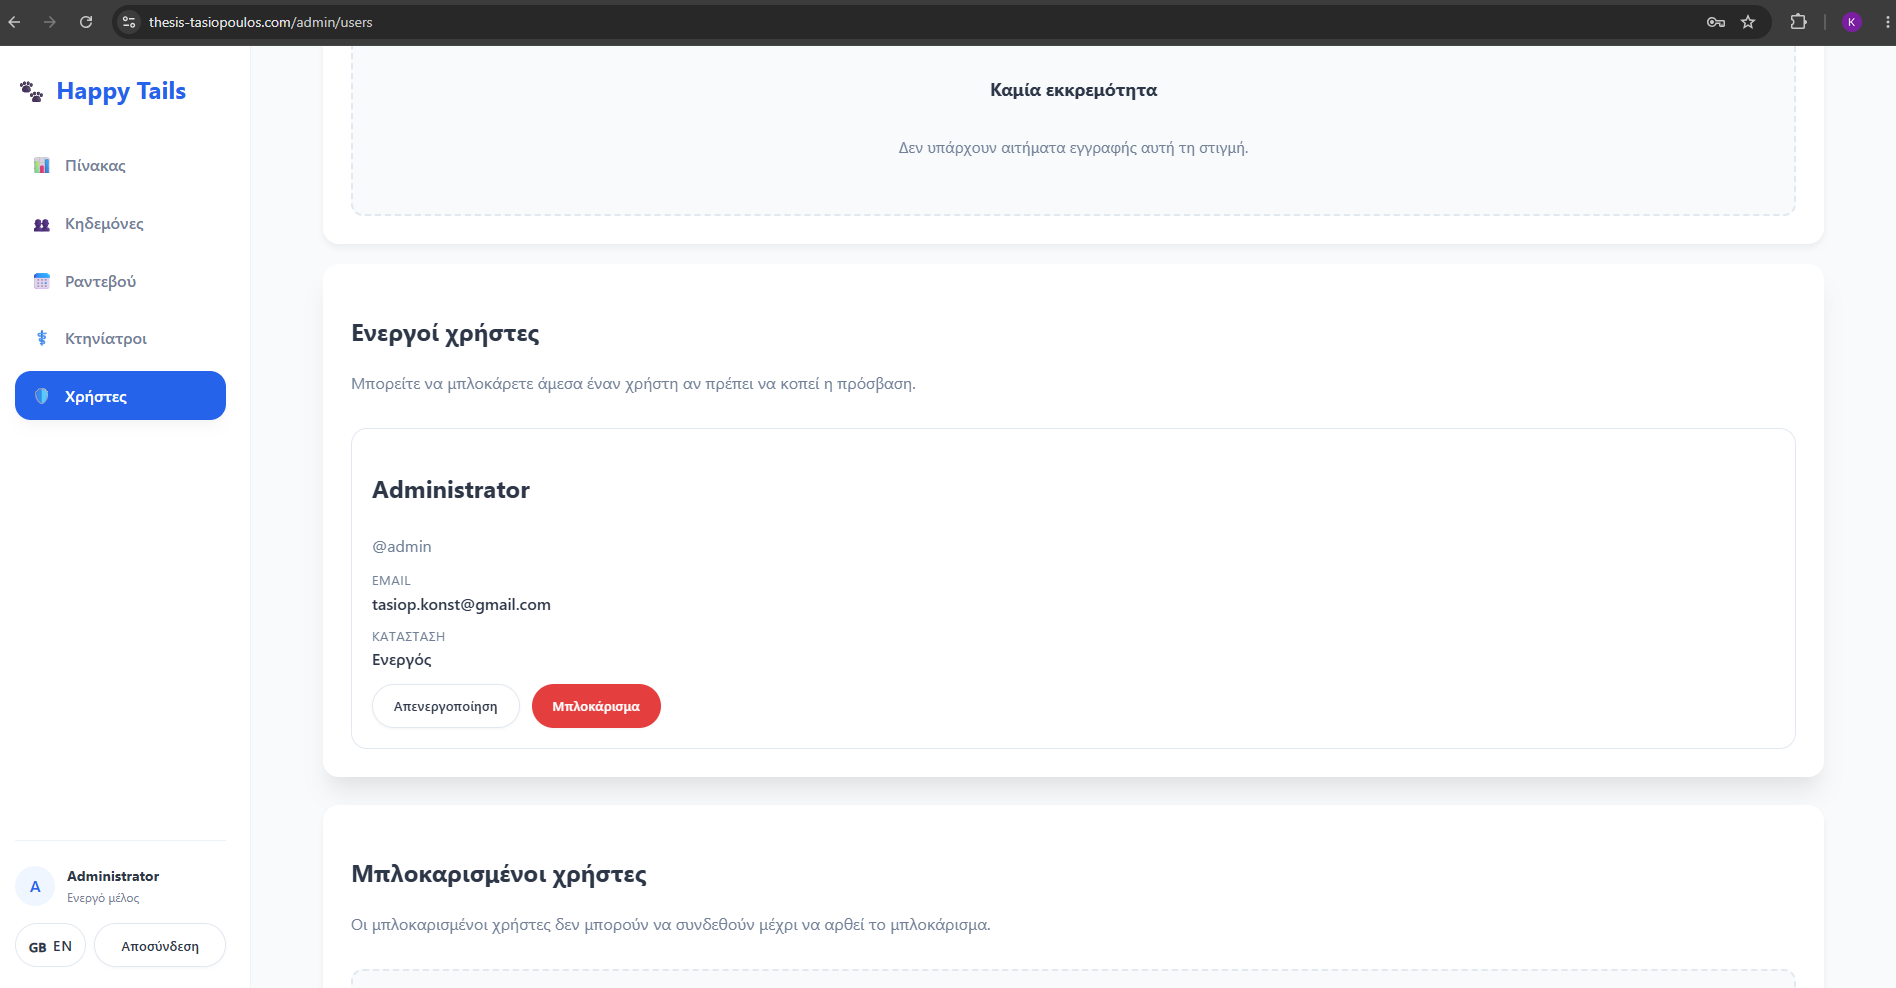
\includegraphics[width=0.9\textwidth]{figures/application/admin-users-desktop.png}
\end{figure}

\section{Εξωτερικές ενσωματώσεις και όρια λειτουργίας}

Η ενσωμάτωση Google Calendar αφορά τον συνδεδεμένο λογαριασμό του μέλους
προσωπικού, όχι το email του ιδιοκτήτη του ζώου. Ο χρήστης εξουσιοδοτεί ρητά
την εφαρμογή μέσω OAuth~2.0 \cite{rfc6749,google2026calendar} και το backend μπορεί κατόπιν να δημιουργεί,
ενημερώνει ή διαγράφει το αντίστοιχο calendar event. Τα δοκιμαστικά
\texttt{example.com} emails των ιδιοκτητών δεν εμποδίζουν αυτή τη ροή,
επειδή χρησιμοποιούνται ως στοιχεία επικοινωνίας και όχι ως λογαριασμοί
πρόσβασης στο ημερολόγιο. Στην παρούσα φάση ο κώδικας υπάρχει, αλλά η
production σύνδεση και η end-to-end δημιουργία event παραμένουν προς τελική
επαλήθευση.

Η υπηρεσία email είναι επίσης προαιρετική εξωτερική εξάρτηση. Η ροή
επιβεβαίωσης έχει υλοποιηθεί στο Spring Boot, όμως η χρήση Amazon SES
\cite{aws2026ses} θα
χαρακτηριστεί ενεργή μόνο μετά τη δημιουργία verified identity και την
επιτυχή παραλαβή μηνύματος από το production περιβάλλον. Η σαφής καταγραφή
αυτών των ορίων αποτρέπει τη σύγχυση ανάμεσα σε δυνατότητα του κώδικα και σε
λειτουργία που έχει ήδη επαληθευτεί στο AWS.

\section{Περιορισμοί της υφιστάμενης εφαρμογής}

Η εφαρμογή καλύπτει ολοκληρωμένα τη βασική ροή, αλλά δεν αποτελεί σύστημα
νοσοκομειακής κλίμακας. Η βάση και τα uploads βρίσκονται στον ίδιο
υπολογιστικό κόμβο, δεν έχει υλοποιηθεί multi-tenant απομόνωση διαφορετικών
κλινικών και δεν υπάρχει πλήρες audit trail κάθε ανάγνωσης ή μεταβολής. Η
responsive διεπαφή έχει ελεγχθεί σε πραγματικό κινητό, όμως απαιτούνται
συστηματικότεροι accessibility και cross-browser έλεγχοι. Επίσης, το
frontend bundle χρειάζεται μελλοντική βελτιστοποίηση και οι εξωτερικές
ενσωματώσεις πρέπει να αξιολογούνται με graceful failure, ώστε μία προσωρινή
αστοχία Google ή email να μην εμποδίζει την κεντρική καταχώριση.

Τα δοκιμαστικά δεδομένα των εικόνων είναι κατάλληλα για επίδειξη της ροής,
όχι για κλινική χρήση. Πριν από παραγωγική αξιοποίηση με πραγματικά δεδομένα
θα απαιτούνταν πληρέστερη πολιτική πρόσβασης, retention, αντιγράφων ασφαλείας
και οργανωτικών διαδικασιών. Οι περιορισμοί αυτοί δεν αναιρούν την
πειραματική αξία του συστήματος· ορίζουν με ακρίβεια το πεδίο στο οποίο
ερμηνεύονται τα αποτελέσματα.

\section{Σύνοψη κεφαλαίου}

Το Happy Tails συνδέει τη δημόσια παρουσίαση με ένα προστατευμένο εργαλείο
κλινικής διαχείρισης. Το React frontend οργανώνει τη ροή και προσαρμόζεται σε
desktop και κινητό, το Spring Boot εφαρμόζει validation, ασφάλεια και
επιχειρησιακή λογική, και η MySQL διατηρεί τις σχέσεις ιδιοκτήτη,
κατοικίδιου, ραντεβού και ιατρικού φακέλου. Τα στιγμιότυπα επιβεβαιώνουν ότι
η πληροφορία ακολουθεί μία συνεχή πορεία από την καταχώριση έως το ημερολόγιο,
το ιστορικό και την εκτύπωση. Με αυτή την εφαρμοστική βάση, το επόμενο
κεφάλαιο μπορεί να εξετάσει τι χρειάζεται ώστε η ίδια λειτουργία να είναι
δημόσια προσβάσιμη και διαχειρίσιμη σε AWS.


\chapter{Σχεδιασμός της Υποδομής Νέφους}
\section{Σχεδιαστικοί στόχοι και παραδοχές}
Η υποδομή σχεδιάστηκε για την ελεγχόμενη φιλοξενία μιας διαδικτυακής
εφαρμογής κτηνιατρικής κλινικής, με βασικούς στόχους τη δυνατότητα
αναπαραγωγής της εγκατάστασης, την ασφαλή απομακρυσμένη διαχείριση, τη
διατήρηση των δεδομένων και τον περιορισμό του λειτουργικού κόστους. Επειδή
το σύστημα αποτελεί πανεπιστημιακό πρωτότυπο με μικρό και προβλέψιμο φορτίο,
προτιμήθηκε αρχικά μια υποδομή ενός υπολογιστικού κόμβου. Η επιλογή αυτή δεν
ισοδυναμεί με αρχιτεκτονική υψηλής διαθεσιμότητας, αλλά επιτρέπει την πλήρη
λειτουργική επίδειξη της εφαρμογής και τη συλλογή μετρήσεων με ελεγχόμενο
κόστος.
\section{Αρχική και προτεινόμενη αρχιτεκτονική}
Η υλοποιημένη αρχιτεκτονική βασίζεται σε ένα EC2 instance στην περιοχή
\texttt{eu-central-1}. Στο EC2 instance εκτελείται Docker Compose με τρεις
υπηρεσίες: Nginx ως reverse proxy, εφαρμογή Spring Boot
και MySQL 8.4. Η επικοινωνία της βάσης δεδομένων και της εφαρμογής παραμένει
στο εσωτερικό δίκτυο του Docker, ενώ προς το Διαδίκτυο εκτίθενται μόνο οι
θύρες του Nginx. Ως αρχιτεκτονική μελλοντικής παραγωγικής λειτουργίας
εξετάζεται ο διαχωρισμός του επιπέδου δεδομένων σε διαχειριζόμενη υπηρεσία
RDS/Aurora, η προσθήκη εξισορρόπησης φορτίου και η λειτουργία σε περισσότερες
της μίας ζώνες διαθεσιμότητας. Οι επεκτάσεις αυτές αξιολογούνται χωριστά και
δεν παρουσιάζονται ως τμήμα της βασικής εγκατάστασης χωρίς αντίστοιχη
πειραματική επαλήθευση.

Ο Πίνακας~\ref{tab:aws-base-configuration} συνοψίζει τη διαμόρφωση που
χρησιμοποιήθηκε στην υλοποιημένη εγκατάσταση. Η συγκεντρωτική παρουσίαση διευκολύνει
την αναπαραγωγή της εγκατάστασης και διαχωρίζει τις πραγματικά υλοποιημένες
επιλογές από τις μελλοντικές αρχιτεκτονικές επεκτάσεις.

\begin{table}[htbp]
\caption{Βασική διαμόρφωση της υλοποιημένης υποδομής AWS.}
\label{tab:aws-base-configuration}
\centering
\begin{tabularx}{\textwidth}{@{}p{3.7cm}X@{}}
\toprule
\textbf{Παράμετρος} & \textbf{Τιμή και αιτιολόγηση} \\
\midrule
AWS Region & \texttt{eu-central-1} (Frankfurt), ώστε οι πόροι της εγκατάστασης να βρίσκονται στην ίδια ευρωπαϊκή περιοχή. \\
EC2 instance & \texttt{t3.small}, 2 vCPU και 2~GiB RAM, ώστε να λειτουργούν ταυτόχρονα JVM, MySQL και Nginx. \\
Λειτουργικό σύστημα & Amazon Linux~2023, συμβατό με Docker και τα εργαλεία διαχείρισης της AWS. \\
Root storage & EBS \texttt{gp3}, 30~GiB, 3.000 baseline IOPS. \\
Network placement & Default VPC και public subnet με route προς Internet Gateway. \\
Public address & Elastic IP \texttt{3.127.189.11}, ώστε η δημόσια διεύθυνση να παραμένει σταθερή. \\
Application runtime & Docker Compose με containers για Spring Boot, MySQL και Nginx. \\
Domain & \texttt{thesis-tasiopoulos.com}, διαχειριζόμενο από Route~53. \\
TLS certificate & Let's Encrypt για root domain και \texttt{www}, με αυτοματοποιημένη ανανέωση. \\
\bottomrule
\end{tabularx}
\end{table}

\begin{figure}[htbp]
\centering
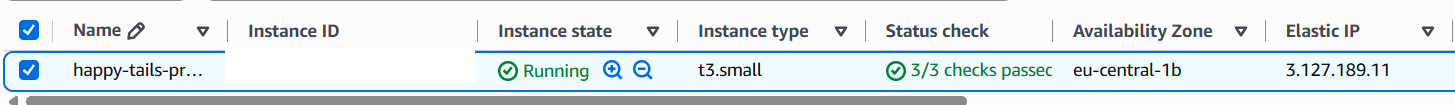
\includegraphics[width=\textwidth]{figures/infrastructure/aws-ec2-instance-summary.png}
\caption[Σύνοψη του υλοποιημένου EC2 instance.]{Σύνοψη του υλοποιημένου EC2 instance. Διακρίνονται η κατάσταση
\texttt{Running}, ο τύπος \texttt{t3.small}, οι επιτυχείς έλεγχοι κατάστασης,
η Availability Zone και η συσχετισμένη Elastic IP. Το μη αναγκαίο instance
identifier έχει αποκρυφθεί.}
\label{fig:aws-ec2-instance-summary}
\end{figure}

\begin{figure}[htbp]
\centering
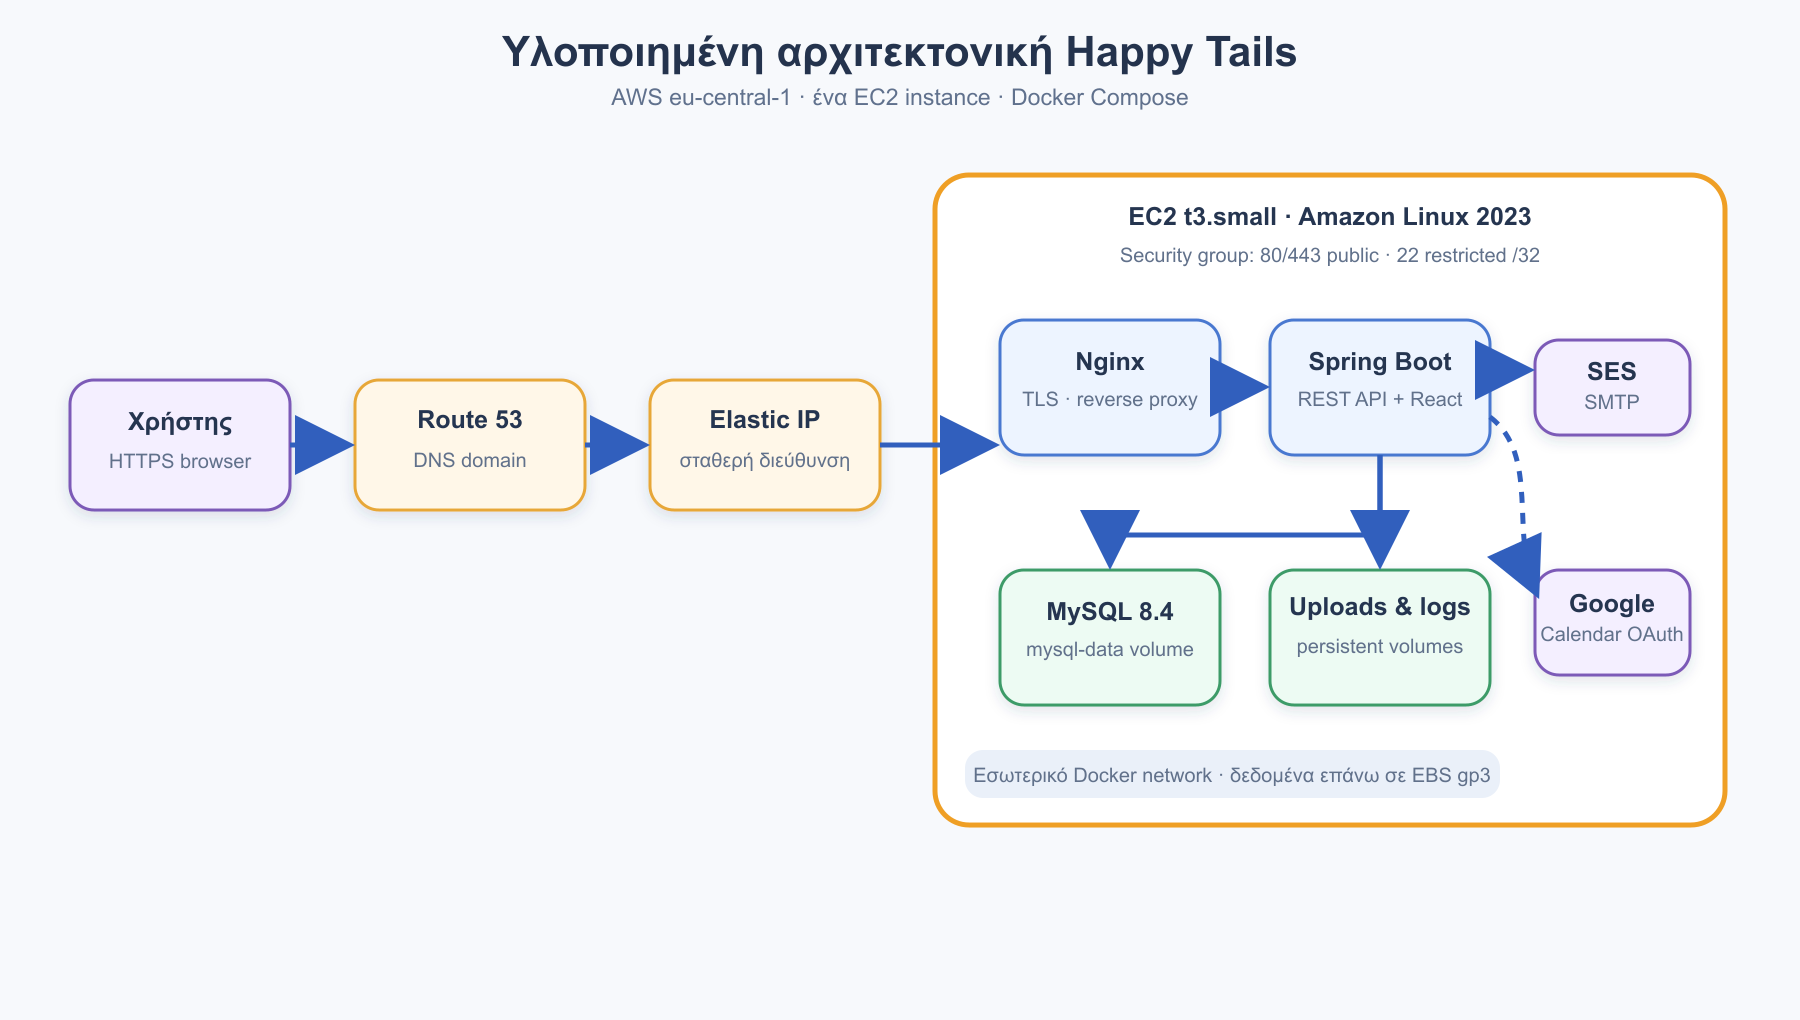
\includegraphics[width=\textwidth]{figures/infrastructure/aws-implemented-architecture.png}
\caption{Αρχιτεκτονική της βασικής εγκατάστασης Happy Tails στο AWS. Η
δημόσια κίνηση καταλήγει μέσω Route~53 και της Elastic IP στον Nginx, ενώ η
εφαρμογή και η MySQL επικοινωνούν αποκλειστικά στο εσωτερικό δίκτυο Docker.
Τα δεδομένα και τα μεταφορτωμένα αρχεία διατηρούνται σε persistent volumes
επάνω στο EBS.}
\label{fig:aws-implemented-architecture}
\end{figure}

\section{Δικτύωση, υποδίκτυα και κανόνες πρόσβασης}
Το EC2 instance τοποθετήθηκε στο default VPC και σε public subnet
της περιοχής της Φρανκφούρτης. Το security group
\texttt{pet-clinic-web-sg} επιτρέπει εισερχόμενη κίνηση στις θύρες 80 και 443
από το Διαδίκτυο. Η θύρα 22 δεν είναι δημόσια διαθέσιμη χωρίς περιορισμό,
αλλά επιτρέπεται μόνο από τη συγκεκριμένη διεύθυνση /32 του διαχειριστή. Με
τον τρόπο αυτό μειώνεται η επιφάνεια επίθεσης, χωρίς να παρεμποδίζεται η
διαχείριση μέσω SSH/SFTP.

\begin{table}[htbp]
\caption{Εισερχόμενοι κανόνες του security group \texttt{pet-clinic-web-sg}.}
\label{tab:security-group-rules}
\centering
\footnotesize
\setlength{\tabcolsep}{4pt}
\begin{tabularx}{0.98\textwidth}{@{}p{1.5cm}p{3.0cm}p{2.5cm}>{\raggedright\arraybackslash}X@{}}
\toprule
\textbf{Υπηρεσία} & \textbf{Πρωτόκολλο και θύρα} & \textbf{Πηγή} & \textbf{Σκοπός} \\
\midrule
HTTP & TCP/80 & \texttt{0.0.0.0/0} & ACME HTTP-01 challenge και ανακατεύθυνση προς HTTPS. \\
HTTPS & TCP/443 & \texttt{0.0.0.0/0} & Κρυπτογραφημένη δημόσια πρόσβαση στην εφαρμογή. \\
SSH & TCP/22 & Συγκεκριμένη IPv4/32 & Περιορισμένη διαχείριση και μεταφορά αρχείων μέσω SSH/SFTP. \\
\bottomrule
\end{tabularx}
\end{table}

\begin{figure}[htbp]
\centering
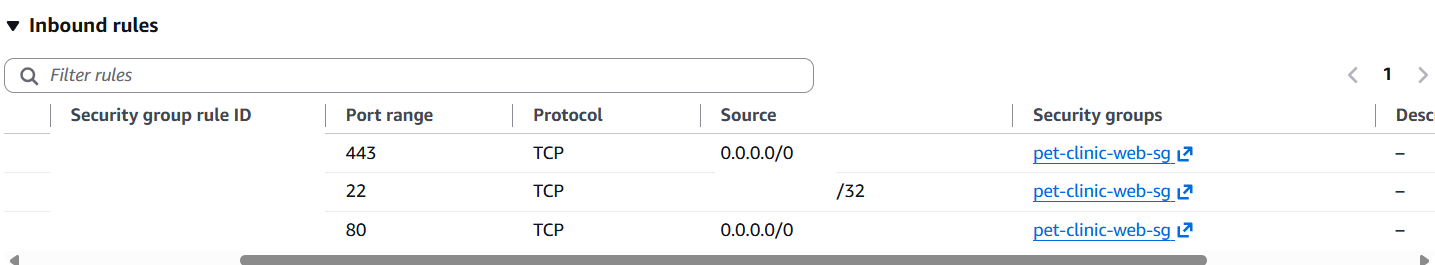
\includegraphics[width=\textwidth]{figures/infrastructure/aws-security-group-inbound.png}
\caption{Inbound rules του security group της εφαρμογής. Οι θύρες 80 και 443
είναι δημόσιες, ενώ για τη θύρα 22 διατηρείται ορατό μόνο το prefix
\texttt{/32}, χωρίς δημοσίευση της διεύθυνσης διαχείρισης.}
\label{fig:aws-security-group-inbound}
\end{figure}
\section{Υπολογιστικό επίπεδο και ανάπτυξη εφαρμογής}
Για το υπολογιστικό επίπεδο επιλέχθηκε EC2 instance type \texttt{t3.small} με δύο
εικονικούς επεξεργαστές και 2~GiB μνήμης. Η επιλογή προσφέρει
περισσότερο περιθώριο από τη διαμόρφωση \texttt{t3.micro} για την ταυτόχρονη
λειτουργία της JVM, της MySQL και του Nginx. Το root EBS volume είναι
τύπου \texttt{gp3}, χωρητικότητας 30~GiB, με τη
βασική επίδοση των 3.000 IOPS.

\begin{figure}[htbp]
\centering
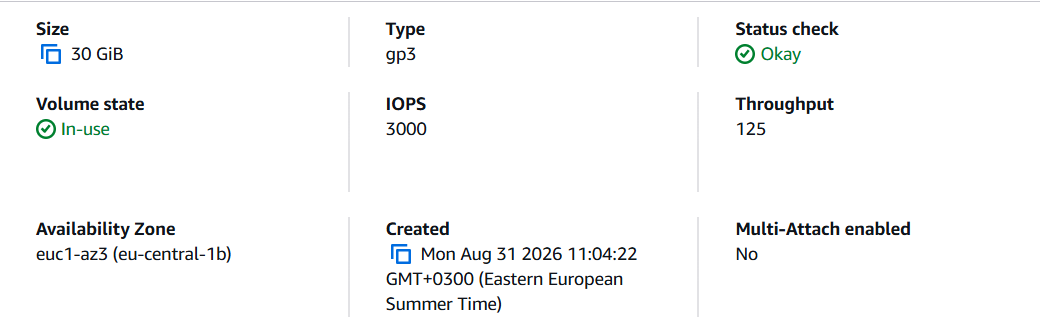
\includegraphics[width=0.9\textwidth]{figures/infrastructure/aws-ebs-volume-configuration.png}
\caption{Βασικά χαρακτηριστικά του EBS volume: χωρητικότητα 30~GiB, τύπος
\texttt{gp3}, 3.000 IOPS, κατάσταση \texttt{In-use} και επιτυχής έλεγχος
κατάστασης.}
\label{fig:aws-ebs-volume-configuration}
\end{figure}
\section{Επίπεδο δεδομένων και στρατηγική αντιγράφων ασφαλείας}
Στη βασική υλοποίηση η MySQL λειτουργεί σε persistent Docker volume επάνω στο
EBS volume, ώστε τα δεδομένα να μη συνδέονται με τον κύκλο ζωής του container.
Η λήψη EBS snapshot εξετάζεται ως περιοδικό αντίγραφο ασφαλείας της
εγκατάστασης και όχι ως μέρος της καθημερινής λειτουργίας. Η χρήση RDS/Aurora εξετάζεται
ως εναλλακτική για διαχειριζόμενα αντίγραφα ασφαλείας και υψηλότερη
διαθεσιμότητα, αλλά συνεπάγεται πρόσθετο σταθερό κόστος.
\section{DNS, πιστοποιητικά και ασφαλής πρόσβαση}
Για τη σταθερή διευθυνσιοδότηση δεσμεύτηκε Elastic IP και συσχετίστηκε με το
EC2 instance. Στο public hosted zone του Route~53 για το
\texttt{thesis-tasiopoulos.com} δημιουργήθηκαν εγγραφές A απλής δρομολόγησης
για το ριζικό όνομα και το \texttt{www}, με TTL 300 δευτερολέπτων. Η
εξωτερική επίλυση DNS επαληθεύτηκε για αμφότερα τα ονόματα. Η τερματική
κρυπτογράφηση TLS πραγματοποιείται στο Nginx με πιστοποιητικό Let's Encrypt
για το ριζικό όνομα και το \texttt{www}, ώστε η εφαρμογή Spring Boot να
παραμένει προσβάσιμη μόνο μέσω του εσωτερικού δικτύου των containers. Η
κίνηση HTTP ανακατευθύνεται υποχρεωτικά σε HTTPS.

\begin{table}[htbp]
\caption{DNS records που χρησιμοποιούνται για τη δημόσια πρόσβαση.}
\label{tab:dns-records}
\centering
\begin{tabularx}{\textwidth}{@{}p{4cm}p{1.6cm}p{3.5cm}X@{}}
\toprule
\textbf{Record name} & \textbf{Type} & \textbf{Value} & \textbf{TTL} \\
\midrule
\texttt{thesis-tasiopoulos.com} & A & \texttt{3.127.189.11} & 300 seconds \\
\texttt{www.thesis-tasiopoulos.com} & A & \texttt{3.127.189.11} & 300 seconds \\
\bottomrule
\end{tabularx}
\end{table}

\begin{figure}[htbp]
\centering
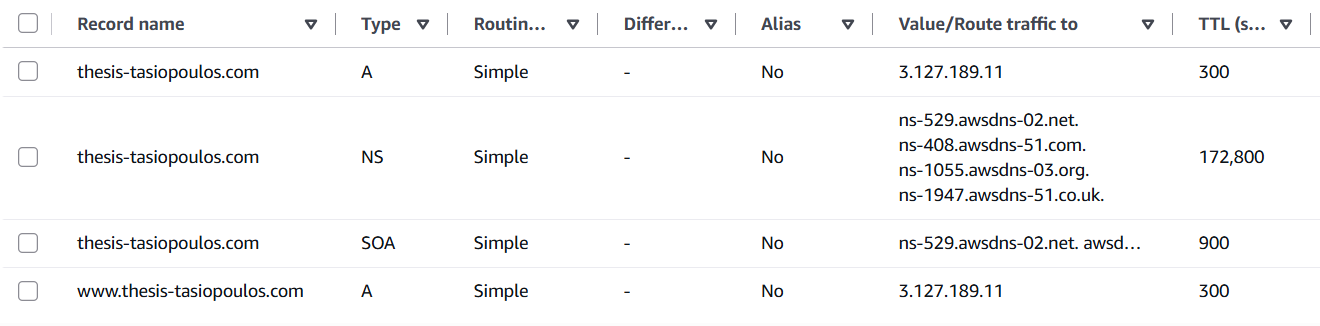
\includegraphics[width=\textwidth]{figures/infrastructure/aws-route53-records.png}
\caption{Εγγραφές Route~53 για το ριζικό όνομα και το \texttt{www}, οι οποίες
κατευθύνονται στην ίδια Elastic IP με TTL 300 δευτερολέπτων.}
\label{fig:aws-route53-records}
\end{figure}

\begin{figure}[htbp]
\centering
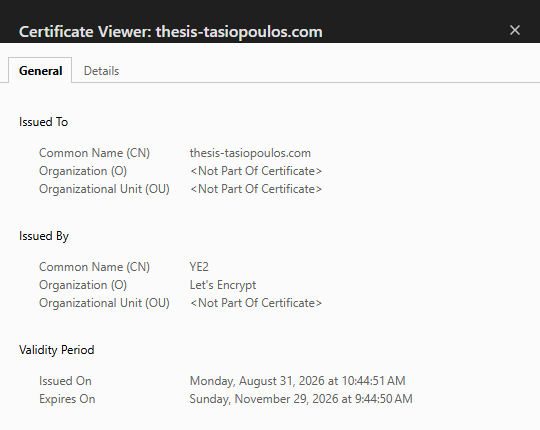
\includegraphics[width=0.62\textwidth]{figures/infrastructure/tls-certificate-validity.png}
\caption{Στοιχεία έκδοσης και χρονικής ισχύος του πιστοποιητικού TLS για το
\texttt{thesis-tasiopoulos.com}. Τα fingerprints δεν περιλαμβάνονται στο
δημοσιευμένο στιγμιότυπο.}
\label{fig:tls-certificate-validity}
\end{figure}

\section{Υπηρεσία αποστολής email με Amazon SES}
Για την αποστολή μηνυμάτων επιβεβαίωσης και επαναφοράς κωδικού των
λογαριασμών προσωπικού
χρησιμοποιήθηκε το Amazon Simple Email Service (SES) στην ίδια περιοχή
\texttt{eu-central-1} με το EC2 instance. Στο SES καταχωρίστηκε ως domain
identity το \texttt{thesis-tasiopoulos.com}. Η κυριότητα του domain και η
δυνατότητα υπογραφής των εξερχόμενων μηνυμάτων επιβεβαιώθηκαν μέσω των DKIM
CNAME records που προστέθηκαν στο Route~53. Μετά τη διάδοση των εγγραφών, η
κατάσταση της ταυτότητας μεταβλήθηκε σε \texttt{Verified}.

Η διεύθυνση αποστολής της εφαρμογής είναι η
\path{no-reply@thesis-tasiopoulos.com}. Η σύνδεση του Spring Boot με το SES
γίνεται μέσω του περιφερειακού SMTP endpoint, στη θύρα 587 με STARTTLS και
authentication. Τα SMTP credentials δημιουργήθηκαν ειδικά για την υπηρεσία
και διατηρούνται μόνο στο προστατευμένο αρχείο environment του EC2 host· δεν
περιλαμβάνονται στο repository, στα screenshots ή στο κείμενο της εργασίας.
Κατά τη δοκιμή το SES παρέμενε σε sandbox mode, με όριο 200 μηνυμάτων ανά
24ωρο και μέγιστο ρυθμό ενός μηνύματος ανά δευτερόλεπτο. Για τον λόγο αυτό
χρησιμοποιήθηκε επαληθευμένος δοκιμαστικός παραλήπτης. Το όριο είναι επαρκές
για την πειραματική αξιολόγηση, αλλά πριν από πραγματική χρήση θα απαιτούνταν
αίτημα production access.

Η επαλήθευση παραλήπτη στο SES sandbox είναι περιορισμός της υποδομής AWS και
δεν ισοδυναμεί με ενεργοποίηση λογαριασμού Happy Tails. Στο δοκιμαστικό
περιβάλλον προηγείται η προσθήκη και επιβεβαίωση της διεύθυνσης του χρήστη
προσωπικού ως SES
identity, ώστε να επιτρέπεται η SMTP παράδοση. Έπειτα ο χρήστης ακολουθεί τον
verification σύνδεσμο του Happy Tails και, τέλος, ο administrator εγκρίνει
την πρόσβαση από την εφαρμογή. Με production access στο SES δεν απαιτείται
επαλήθευση κάθε παραλήπτη, ενώ εξακολουθούν να απαιτούνται verified sender
identity και οι δύο έλεγχοι του Happy Tails. Οι διευθύνσεις των
πελατών/κηδεμόνων δεν αποτελούν παραλήπτες του SES σε αυτή την
αρχιτεκτονική.

Πριν συνδεθεί η υπηρεσία με τη ροή εγγραφής πραγματοποιήθηκε ανεξάρτητη
δοκιμαστική αποστολή από την κονσόλα SES. Η Εικόνα~\ref{fig:amazon-ses-evidence}
συνδέει την επαληθευμένη domain identity με το μήνυμα που παραδόθηκε επιτυχώς.
Το ARN και το AWS account identifier έχουν αφαιρεθεί, ενώ το δημόσιο domain,
η περιοχή και η κατάσταση επαλήθευσης παραμένουν ορατά επειδή τεκμηριώνουν
τη διαμόρφωση.

\begin{figure}[htbp]
\centering
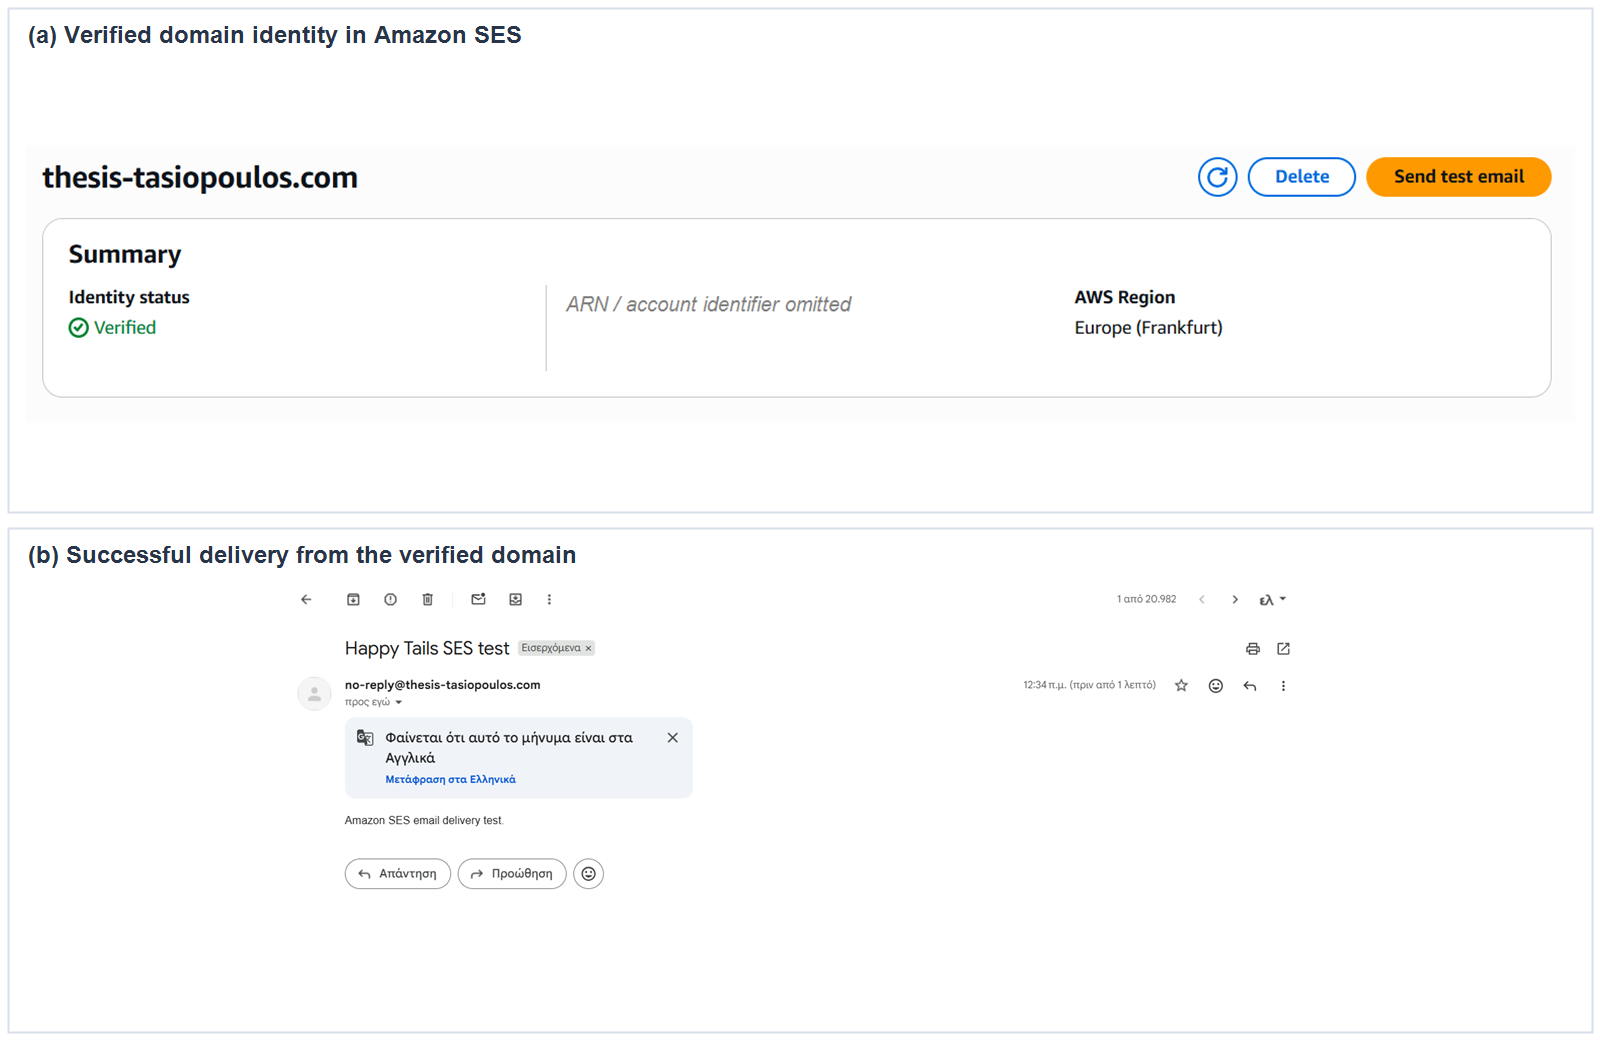
\includegraphics[width=\textwidth]{figures/infrastructure/amazon-ses-verification-and-delivery.png}
\caption{Επαλήθευση της domain identity στο Amazon SES και επιτυχής
δοκιμαστική παράδοση μηνύματος από το επαληθευμένο domain.}
\label{fig:amazon-ses-evidence}
\end{figure}
\section{Παρακολούθηση, καταγραφή και ειδοποιήσεις}
Η παρακολούθηση οργανώθηκε σε επίπεδα, ώστε ένα πρόβλημα να μπορεί να
εντοπιστεί χωρίς να συγχέεται η κατάσταση του εικονικού μηχανήματος με την
κατάσταση της εφαρμογής. Στο επίπεδο AWS, το CloudWatch συλλέγει αυτόματα τα
βασικά metrics του EC2 instance, όπως χρήση CPU, εισερχόμενη και εξερχόμενη
κίνηση δικτύου και αποτυχίες των status checks. Τα metrics αυτά δεν απαιτούν
τροποποίηση του κώδικα και επαρκούν για να διαπιστωθεί αν το instance
λειτουργεί, αν παρουσιάζει ασυνήθιστα υψηλό υπολογιστικό φορτίο ή αν έχει
χαθεί η δικτυακή του διαθεσιμότητα. Η μνήμη και η πληρότητα του file system
δεν περιλαμβάνονται στα προεπιλεγμένα EC2 metrics και θα απαιτούσαν
CloudWatch Agent· για τον λόγο αυτό δεν θεωρούνται διαθέσιμες μετρήσεις χωρίς
προηγούμενη εγκατάσταση και επαλήθευση του agent.

Στο λειτουργικό επίπεδο ελέγχεται η υπηρεσία Docker και η κατάσταση των
containers. Η MySQL διαθέτει health check, από το οποίο εξαρτάται η εκκίνηση
του Spring Boot container. Η πολιτική \texttt{restart: unless-stopped}
εφαρμόζεται και στις τρεις υπηρεσίες, επιτρέποντας την αυτόματη επαναφορά τους
μετά από επανεκκίνηση του host ή μη αναμενόμενο τερματισμό. Οι έλεγχοι
\texttt{docker compose ps}, το health status της MySQL και μία τοπική αίτηση
HTTP προς τον Nginx δίνουν μία σύντομη αλλά πρακτική εικόνα της συνολικής
αλυσίδας λειτουργίας.

Η εφαρμογή Spring Boot γράφει το αρχείο καταγραφής
\path{/app/logs/petclinic.log}, το οποίο βρίσκεται σε persistent Docker
volume. Παράλληλα, τα standard output και error streams παραμένουν διαθέσιμα
μέσω των Docker logs. Ο Nginx διατηρεί access και error logs, ώστε να είναι
δυνατή η συσχέτιση ενός δημόσιου HTTP αιτήματος με την αντίστοιχη λειτουργία
του backend. Στην παρούσα εγκατάσταση τα application και proxy logs
παραμένουν στο EC2 instance. Η συγκεντρωτική αποστολή τους στο CloudWatch
Logs αποτελεί εύλογη επέκταση, αλλά δεν παρουσιάζεται ως ήδη ενεργή
λειτουργία.

Για τη χρονική περίοδο των πειραμάτων προβλέπεται dashboard με τα metrics
\path{CPUUtilization}, \path{NetworkIn}, \path{NetworkOut} και
\path{StatusCheckFailed}, καθώς και alarm για αποτυχία status check ή
παρατεταμένη υψηλή χρήση CPU. Η ακριβής διάρκεια, το threshold και το
διάστημα αξιολόγησης θα καταγραφούν μαζί με τα αποτελέσματα στο
Κεφάλαιο~6. Με αυτόν τον διαχωρισμό, το παρόν κεφάλαιο περιγράφει τον
μηχανισμό παρακολούθησης, ενώ το κεφάλαιο αξιολόγησης παρουσιάζει τις
πραγματικές μετρήσεις και την ερμηνεία τους.
\section{Ασφάλεια και διαχείριση μυστικών}
Η ασφάλεια αντιμετωπίζεται ως βασική απαίτηση ορθής λειτουργίας της cloud
υποδομής και όχι ως αυτοτελές αντικείμενο κυβερνοασφάλειας. Τα ports HTTP και
HTTPS είναι δημόσια, ενώ η πρόσβαση SSH περιορίζεται στη διεύθυνση του
διαχειριστή και η MySQL προσδένεται μόνο στο loopback interface του EC2 host.
Η επικοινωνία του χρήστη τερματίζεται στο Nginx μέσω TLS και τα προστατευμένα
API endpoints απαιτούν authentication και role-based authorization.

Τα database passwords, το JWT signing secret, το bootstrap administrator
password και τα προαιρετικά OAuth credentials δεν αποθηκεύονται στον πηγαίο
κώδικα. Παρέχονται κατά το deployment μέσω τοπικού αρχείου environment, το
οποίο εξαιρείται από το version control και προστατεύεται με δικαιώματα του
λειτουργικού συστήματος. Η προσέγγιση αυτή είναι επαρκής για την υλοποιημένη
πειραματική εγκατάσταση, ενώ η χρήση AWS Systems Manager Parameter Store ή
AWS Secrets Manager εξετάζεται ως μελλοντική managed εναλλακτική.

\section{Αξιολόγηση εναλλακτικών και εκτίμηση κόστους}
Η βασική υλοποίηση διατηρεί μία EC2 instance ώστε το λειτουργικό και οικονομικό
αποτύπωμα να παραμένει ελεγχόμενο. Συμπληρωματικά θα εξεταστούν, με σύντομο
proof of concept όπου το επιτρέπει το κόστος, ένα Application Load Balancer
(ALB)
ως σταθερό σημείο εισόδου και το CloudFront ως edge distribution
layer~\cite{aws2026cloudfront}. Η
δυνατότητα σύνδεσης AWS WAF σε ALB ή CloudFront, καθώς και η μεταφορά της
βάσης σε RDS/Aurora, θα παρουσιαστούν ως εναλλακτικές υψηλότερης
διαθεσιμότητας και διαχειρισιμότητας. Κάθε υπηρεσία θα χαρακτηρίζεται ρητά ως
υλοποιημένη, προσωρινά δοκιμασμένη ή προτεινόμενη, χωρίς να εντάσσεται τεχνητά
στο κύριο deployment.

\begin{table}[htbp]
\caption{Κατάσταση των βασικών υπηρεσιών και integrations κατά τη συγγραφή.}
\label{tab:service-status}
\centering
\begin{tabularx}{\textwidth}{@{}p{3.3cm}p{3.3cm}X@{}}
\toprule
\textbf{Υπηρεσία ή στοιχείο} & \textbf{Κατάσταση} & \textbf{Υφιστάμενο ή απαιτούμενο τεκμήριο} \\
\midrule
EC2, EBS και Elastic IP & Υλοποιημένα & Ενεργό instance, volume και σταθερή δημόσια διεύθυνση. \\
Route~53, Nginx και HTTPS & Υλοποιημένα & DNS records, HTTP~301, HTTPS~200 και έγκυρο TLS certificate. \\
Docker Compose και MySQL & Υλοποιημένα & Τρία ενεργά containers και επιτυχής database health check. \\
Google Calendar OAuth & Υλοποιημένο και επαληθευμένο & Επιτυχής production σύνδεση και end-to-end έλεγχος δημιουργίας, ενημέρωσης και διαγραφής event με ειδοποίηση attendees. \\
Amazon SES & Υλοποιημένο και επαληθευμένο σε sandbox & Verified domain και δοκιμαστικός παραλήπτης, επιτυχής SMTP αποστολή και end-to-end έλεγχοι εγγραφής και επαναφοράς κωδικού. \\
ALB & Υποψήφιο για περιορισμένο test & Θα χαρακτηριστεί ως δοκιμασμένο μόνο αν δημιουργηθεί και καταγραφεί proof of concept. \\
CloudFront & Προσωρινά δοκιμασμένο & Απομονωμένο proof of concept μέσω του προεπιλεγμένου hostname, χωρίς αλλαγή του production DNS. \\
RDS/Aurora, WAF και Secrets Manager & Προτεινόμενα & Θεωρητική αξιολόγηση οφέλους, περιορισμών και κόστους. \\
\bottomrule
\end{tabularx}
\end{table}



\chapter{Υλοποίηση και Ανάπτυξη}
\section{Περιβάλλον ανάπτυξης και εργαλεία}
Η εφαρμογή αναπτύχθηκε με Spring Boot και React, ενώ για τη σχεσιακή
αποθήκευση χρησιμοποιείται MySQL. Η συσκευασία και η εκτέλεση των επιμέρους
υπηρεσιών βασίζονται σε Docker και Docker Compose. Για τη διαχείριση αρχείων
και την ασφαλή απομακρυσμένη πρόσβαση χρησιμοποιούνται SSH/SFTP και
Cyberduck, ενώ η διαχείριση των πόρων νέφους πραγματοποιείται από την κονσόλα
AWS.
\section{Δημιουργία και διαχείριση εικόνων Docker}
Η εγκατάσταση περιλαμβάνει τρία containers: \texttt{petclinic-mysql} με
MySQL~8.4, \texttt{petclinic-app} με την εφαρμογή Spring Boot και
\texttt{petclinic-nginx} με Nginx~1.27 Alpine. Οι υπηρεσίες φέρουν πολιτική
\texttt{restart: unless-stopped}. Η υπηρεσία Docker ρυθμίστηκε να εκκινεί
μαζί με το λειτουργικό σύστημα. Έτσι, μετά από reboot του EC2 instance, η
πολιτική επανεκκίνησης ενεργοποιεί αυτόματα και τα τρία containers.

\begin{figure}[htbp]
\centering
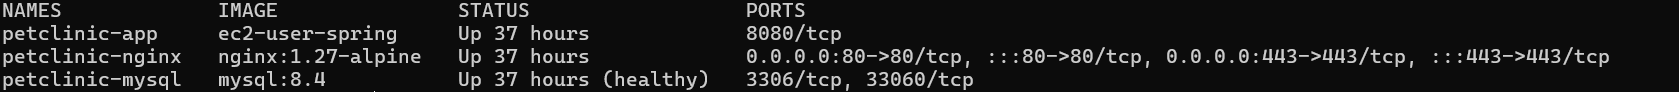
\includegraphics[width=\textwidth]{figures/infrastructure/docker-running-containers.png}
\caption{Κατάσταση των containers της παραγωγικής εγκατάστασης. Η εφαρμογή,
ο Nginx και η MySQL εκτελούνται ταυτόχρονα, ενώ η MySQL αναφέρεται ως
\texttt{healthy}.}
\label{fig:docker-running-containers}
\end{figure}
\section{Παραμετροποίηση της εφαρμογής ανά περιβάλλον}
Τα στοιχεία σύνδεσης της βάσης δεδομένων, το JWT signing secret, το bootstrap
password και τα credentials εξωτερικών υπηρεσιών παρέχονται μέσω environment
variables. Το πραγματικό αρχείο \texttt{.env} δεν συμπεριλαμβάνεται στο
version control, ενώ στο repository διατηρείται μόνο αρχείο παραδείγματος με
τα ονόματα των απαιτούμενων μεταβλητών. Με τον τρόπο αυτό το ίδιο application
package μπορεί να χρησιμοποιείται σε local και production περιβάλλον χωρίς
ενσωμάτωση μυστικών στον πηγαίο κώδικα.

\section{Ενσωμάτωση Google Calendar και Amazon SES}
Η εφαρμογή υποστηρίζει σύνδεση λογαριασμού Google Calendar μέσω OAuth~2.0.
Μετά από ρητή εξουσιοδότηση του χρήστη, τα ραντεβού μπορούν να
αντιστοιχίζονται με calendar events. Το OAuth client identifier και το client
secret δεν αποθηκεύονται στον κώδικα, αλλά παρέχονται κατά το deployment μέσω
environment variables, μαζί με το εγκεκριμένο callback URL του production
domain. Για την ελεγχόμενη δοκιμή δημιουργήθηκε ανεξάρτητο Google Cloud
project, ενεργοποιήθηκε το Google Calendar API και διαμορφώθηκε εφαρμογή
OAuth τύπου External σε κατάσταση Testing. Ο λογαριασμός του έργου ορίστηκε
ως ο μοναδικός test user και ο Web OAuth client δέχεται ως redirect URI το
\path{https://thesis-tasiopoulos.com/auth/google/callback}. Τα νέα
credentials αποθηκεύτηκαν εκτός repository και δεν εμφανίζονται στα τεκμήρια.
Στο production περιβάλλον μεταφέρθηκαν μέσω κρυφής εισόδου τερματικού στο
προστατευμένο αρχείο \texttt{.env} και αντιστοιχίστηκαν αποκλειστικά στο Spring
container μέσω Docker Compose. Μετά την επαναδημιουργία μόνο του Spring
container επαληθεύτηκαν η παρουσία των τριών μεταβλητών, η επιτυχής εκκίνηση
της εφαρμογής και απόκριση HTTP~200 από το δημόσιο HTTPS endpoint.

Η λειτουργία εκτίθεται από τη σελίδα \enquote{Profile \& Integrations}, στην
οποία ο χρήστης μεταβαίνει και από την κάρτα ονόματος και avatar της
πλευρικής πλοήγησης. Η σελίδα διαχωρίζει σκόπιμα δύο έννοιες: το email
επικοινωνίας του λογαριασμού Happy Tails και το email του εξουσιοδοτημένου
Google Calendar. Το πρώτο εξακολουθεί να υπόκειται στον μοναδικό περιορισμό
της βάσης δεδομένων, ενώ το δεύτερο αποθηκεύεται στο ξεχωριστό πεδίο
\texttt{calendarEmail}. Επομένως ένας ήδη χρησιμοποιούμενος Google λογαριασμός
μπορεί να συνδεθεί ως πάροχος ημερολογίου χωρίς να μετονομάσει τον χρήστη ή να
συγκρουστεί με το email άλλου application account, όπως του administrator.

Με την επιλογή \enquote{Connect Google Calendar} το backend δημιουργεί τυχαία
τιμή \texttt{state}, τη συνδέει με τον ενεργό χρήστη σε βραχύβιο server-side
session και ανακατευθύνει στη σελίδα συγκατάθεσης της Google. Ζητούνται τα
scopes Calendar, OpenID, email και profile. Στην επιστροφή, το callback
ελέγχει κωδικό και \texttt{state} πριν ανταλλάξει τον authorization code με
access και refresh token. Τα tokens δεν επιστρέφονται στο React frontend και
δεν εμφανίζονται στα στιγμιότυπα. Η διαδρομή αποτελέσματος OAuth επιτρέπεται
να φορτωθεί δημόσια ώστε να εμφανίσει το αποτέλεσμα της εξωτερικής
ανακατεύθυνσης, ενώ η επόμενη μετάβαση στο profile προστατεύεται κανονικά από
το JWT cookie. Το session cookie έχει \texttt{HttpOnly}, \texttt{Secure} και
\texttt{SameSite=Lax}, ώστε να διατηρείται ο έλεγχος \texttt{state} κατά την
επιστροφή από τη Google χωρίς να γίνεται προσβάσιμο από JavaScript.

Μετά τη σύνδεση, η δημιουργία ραντεβού επιχειρεί εισαγωγή event, η αλλαγή
ημερομηνίας ή στοιχείων εκτελεί patch και η διαγραφή ραντεβού διαγράφει το
αντίστοιχο event. Το αναγνωριστικό του Google event αποθηκεύεται στο
ραντεβού, ώστε η εφαρμογή να γνωρίζει αν απαιτείται δημιουργία ή ενημέρωση.
Επειδή τα ραντεβού αποθηκεύονται ως τοπικές τιμές χωρίς offset, η μετατροπή
προς και από Google Calendar χρησιμοποιεί ρητά την IANA ζώνη
\texttt{Europe/Athens}, μαζί με τους κανόνες θερινής ώρας, και όχι την
προεπιλεγμένη ζώνη UTC του container. Η Google χρησιμοποιεί την ίδια χρονική
πληροφορία για την εμφάνιση του event και για τις προσκλήσεις που αποστέλλει
στους attendees· η εφαρμογή δεν δημιουργεί δεύτερο αρχείο iCalendar μέσω SES.

Η τελική δοκιμή επιβεβαίωσε ότι το ίδιο ραντεβού εμφανίζεται στις 09:30 τόσο
στην εφαρμογή (Σχήμα~\ref{fig:calendar-app-time}) όσο και στο Google Calendar,
ενώ η πρόσκληση αναγράφει επίσης 09:30--10:00 και τη ζώνη Eastern European
Time--Athens (Σχήμα~\ref{fig:calendar-google-evidence}).

\begin{figure}[htbp]
\centering
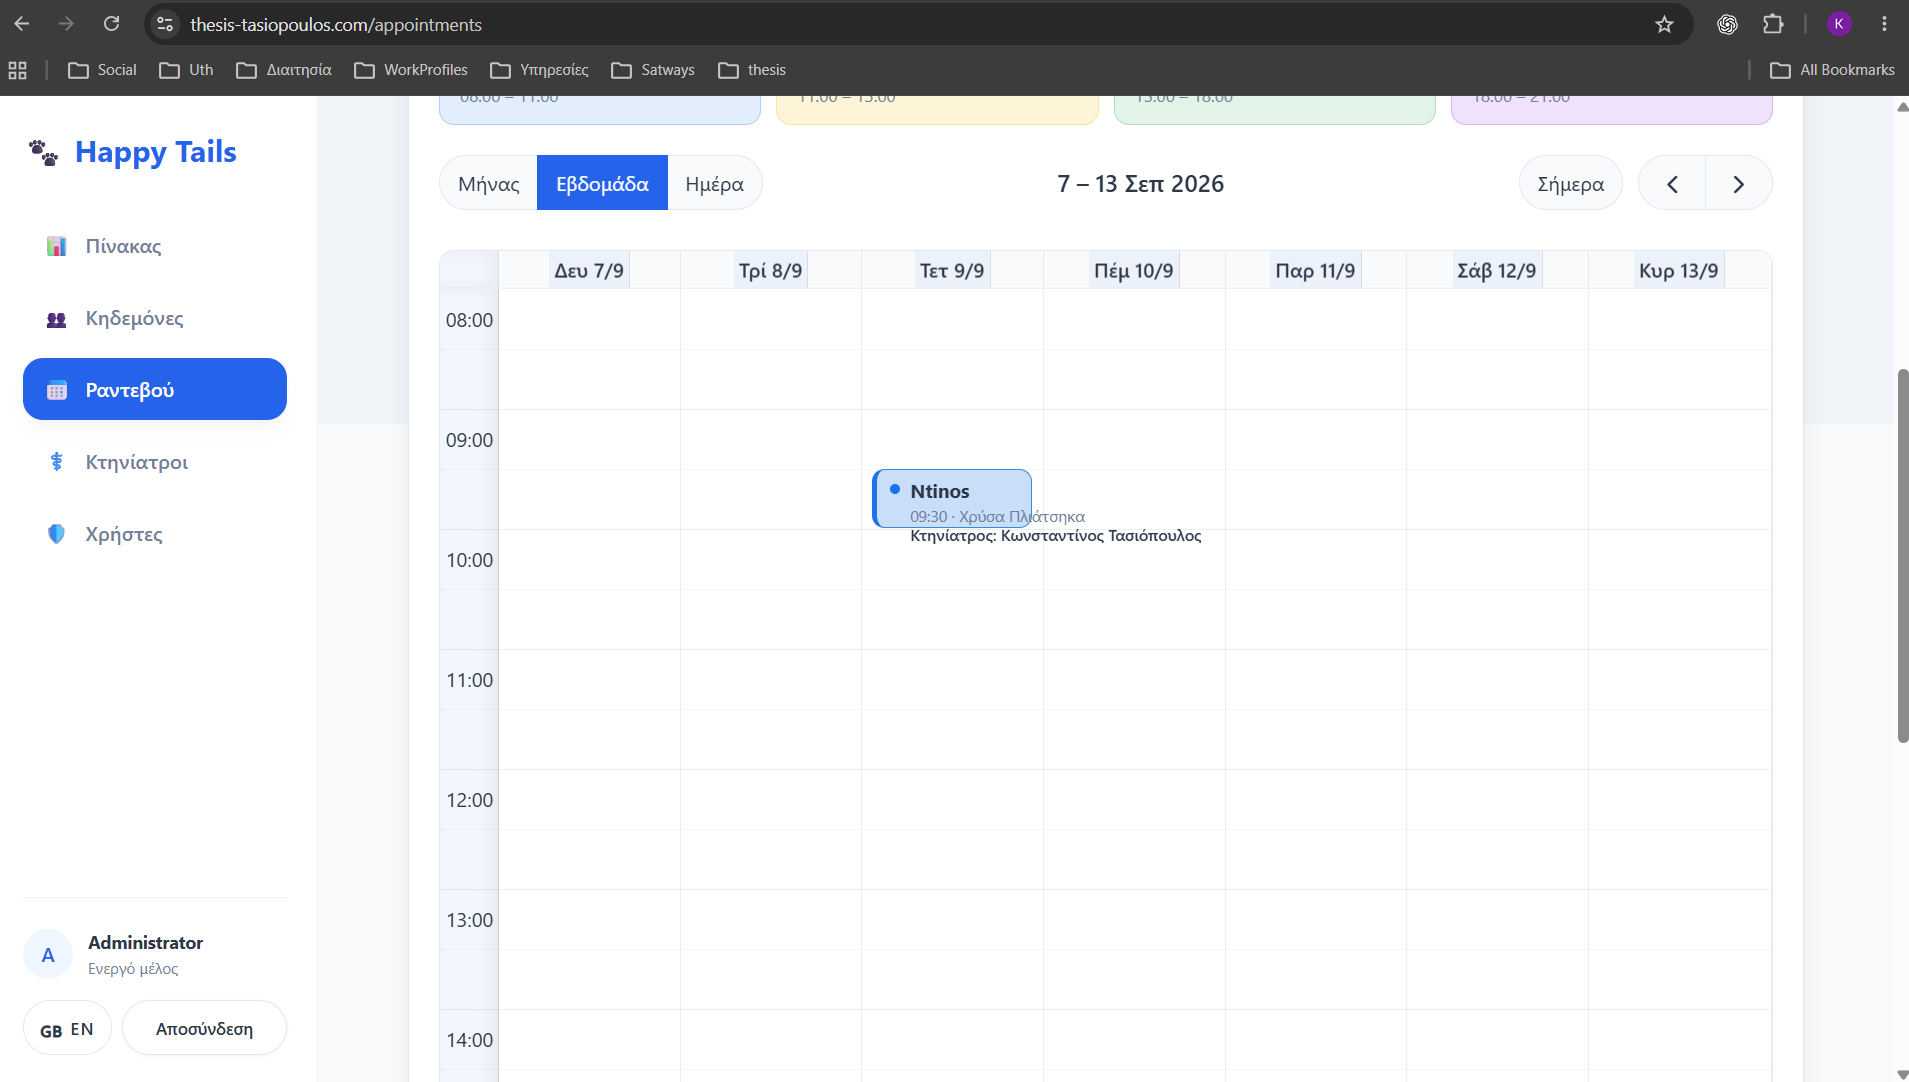
\includegraphics[width=0.96\textwidth]{figures/application/google-calendar-app-0930.png}
\caption{Το δοκιμαστικό ραντεβού στις 09:30 στην εβδομαδιαία προβολή του
Happy Tails μετά τη διόρθωση της ζώνης ώρας.}
\label{fig:calendar-app-time}
\end{figure}

\begin{figure}[htbp]
\centering
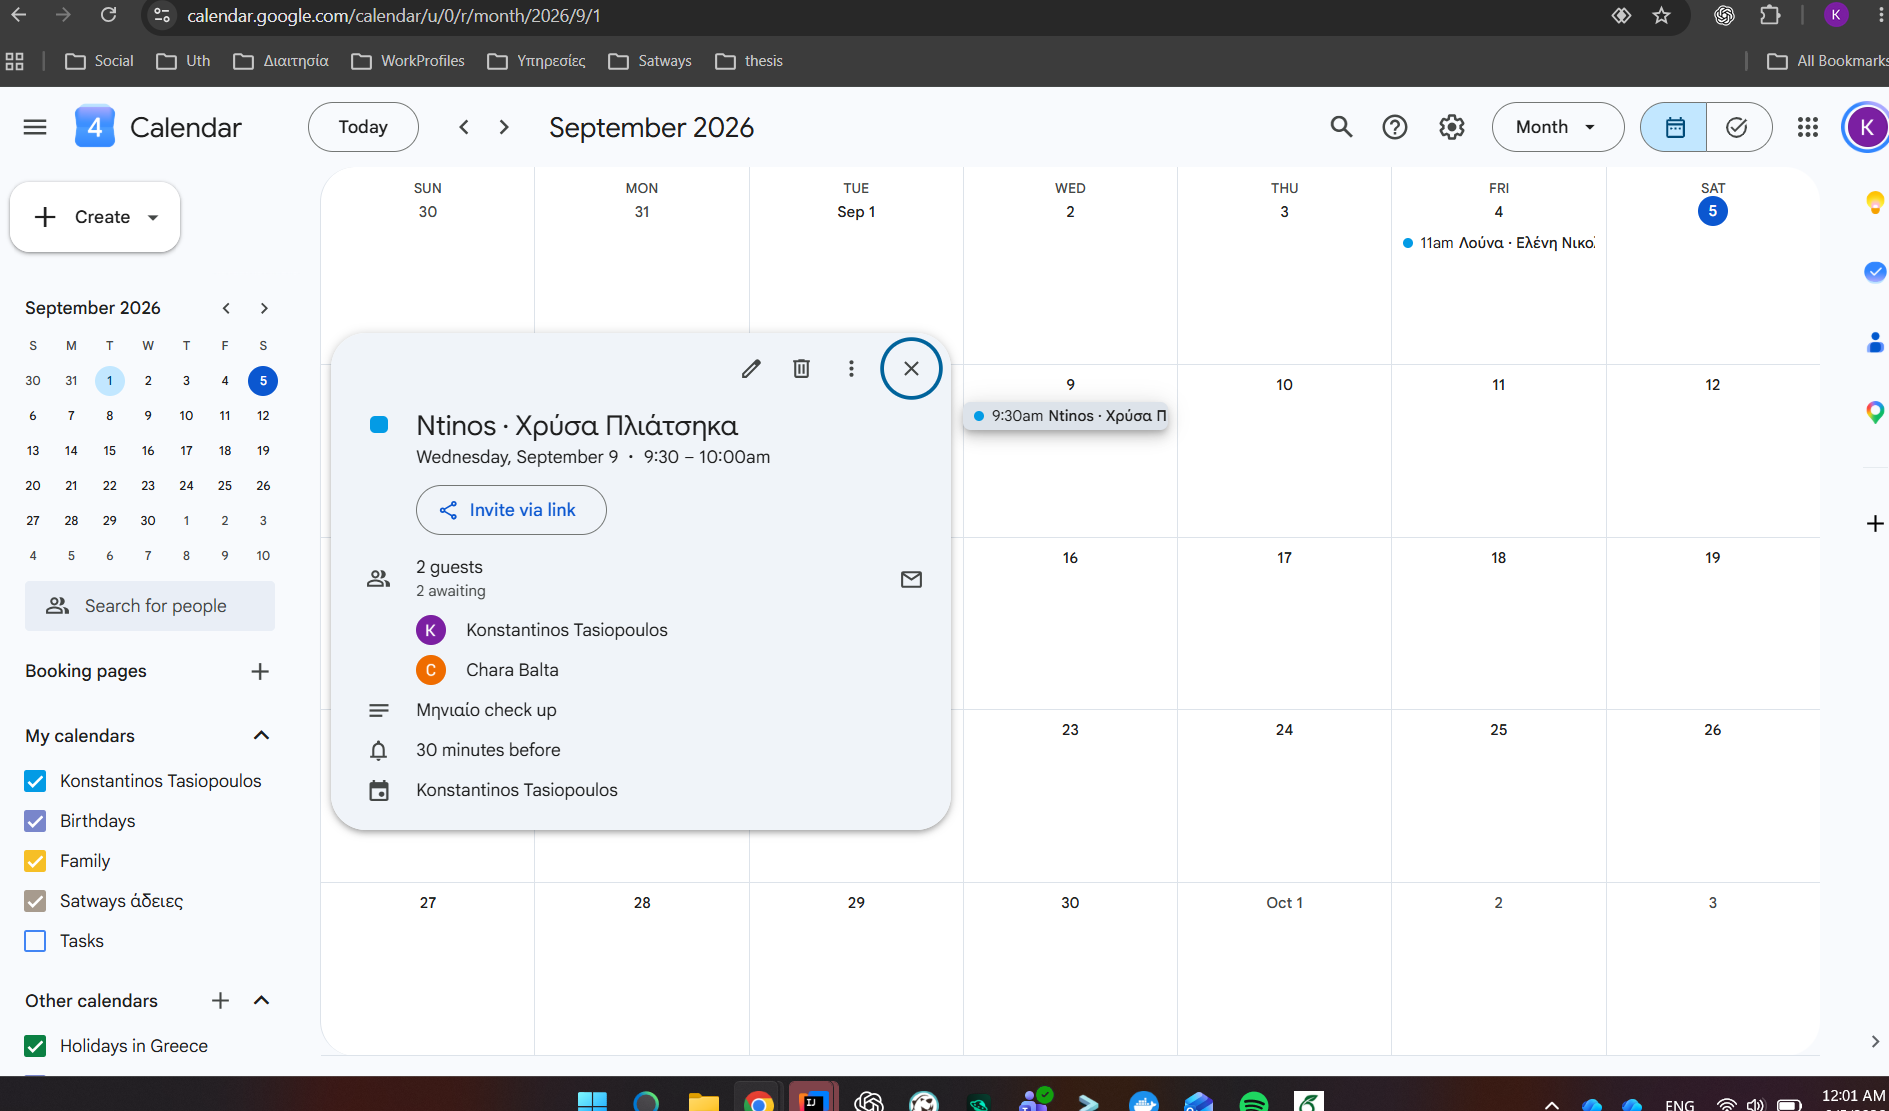
\includegraphics[width=0.78\textwidth]{figures/application/google-calendar-event-0930.png}\par\medskip
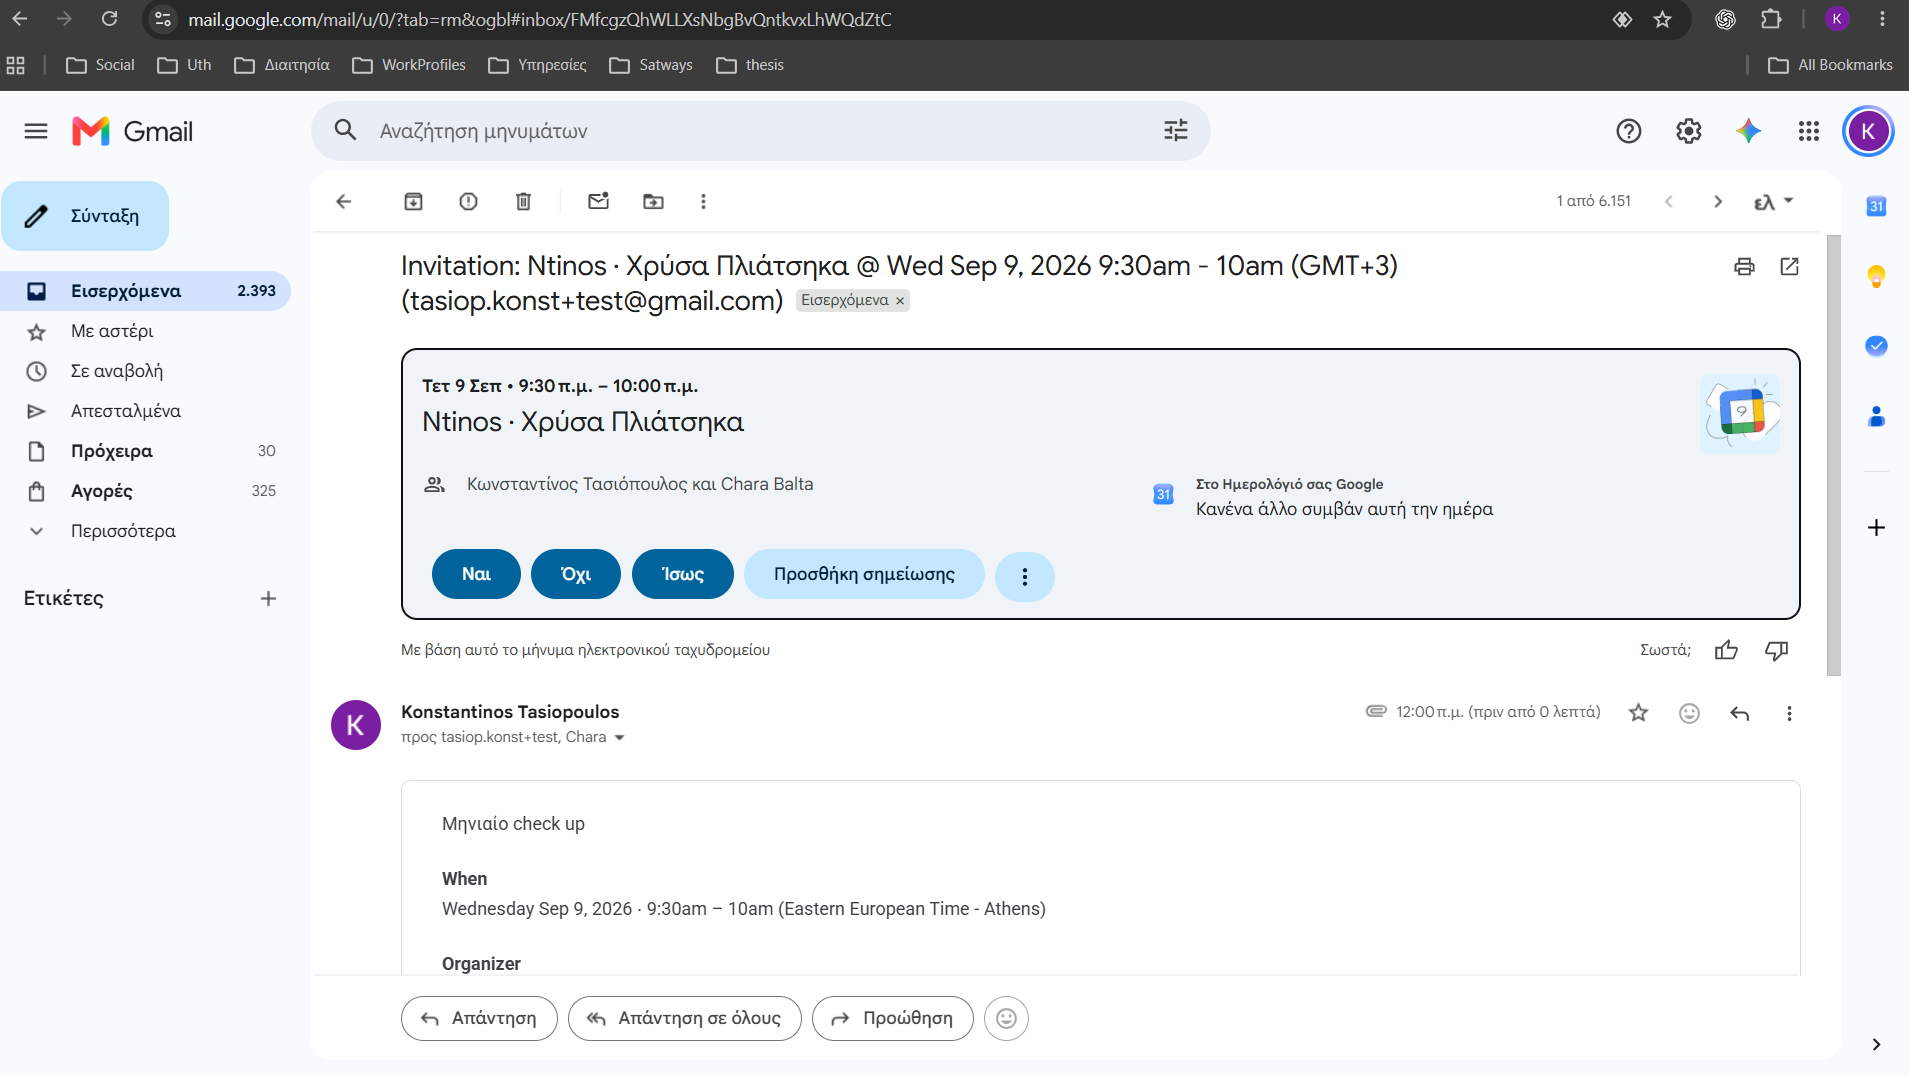
\includegraphics[width=0.78\textwidth]{figures/application/google-calendar-invitation-email.png}
\caption{Το ίδιο event στο Google Calendar και η αντίστοιχη πρόσκληση email,
με συμφωνία ώρας 09:30 και διάρκεια τριάντα λεπτών. Ο administrator/organizer
και η client owner αποτελούν διαφορετικούς δοκιμαστικούς παραλήπτες.}
\label{fig:calendar-google-evidence}
\end{figure}

Το Amazon SES και το Google Calendar αποτελούν δύο ανεξάρτητες εξωτερικές
ενσωματώσεις και δεν επικοινωνούν απευθείας μεταξύ τους. Το Happy Tails είναι
το κοινό σημείο ενορχήστρωσης, αλλά τους αναθέτει διαφορετικές ευθύνες. Η
υπηρεσία Calendar καλεί το Google Calendar API με OAuth tokens για create,
patch ή delete του event και χρησιμοποιεί \texttt{sendUpdates=all}, οπότε η
ίδια η Google αποστέλλει προσκλήσεις, ενημερώσεις και ακυρώσεις στους
attendees. Το Amazon SES δεν συμμετέχει στη ροή ραντεβού· χρησιμοποιείται
αποκλειστικά για verification και password reset των λογαριασμών προσωπικού
της εφαρμογής.

Ο Πίνακας~\ref{tab:external-notification-triggers} αποσαφηνίζει πότε
ενεργοποιείται κάθε μηχανισμός. Ο διαχωρισμός αποτρέπει διπλές ειδοποιήσεις
και δεν υποχρεώνει τους πελάτες να διαθέτουν λογαριασμό Happy Tails ή verified
SES identity.

\begin{table}[htbp]
\centering
\caption{Διάκριση trigger, καναλιού και παραληπτών για Google Calendar και
Amazon SES.}
\label{tab:external-notification-triggers}
\small
\begin{tabularx}{\textwidth}{p{0.19\textwidth} X X}
\toprule
\textbf{Trigger} & \textbf{Google Calendar} & \textbf{Amazon SES} \\
\midrule
Νέος λογαριασμός & Δεν ενεργοποιείται. & Στέλνει verification link διάρκειας
24 ωρών στο email του νέου application user. \\
Αίτημα επαναφοράς κωδικού & Δεν ενεργοποιείται. & Στέλνει link διάρκειας
60 λεπτών στο email υπάρχοντος, επιβεβαιωμένου application user. \\
Δημιουργία ραντεβού & Εισάγει event και η Google ειδοποιεί τους attendees. &
Δεν ενεργοποιείται. \\
Ενημέρωση ή μεταφορά & Εκτελεί patch του event και ενημερώνει attendees. &
Δεν ενεργοποιείται. \\
Διαγραφή ραντεβού & Διαγράφει το event και η Google στέλνει cancellation. &
Δεν ενεργοποιείται. \\
Διοικητική έγκριση λογαριασμού & Δεν ενεργοποιείται. & Δεν αποστέλλεται
ξεχωριστό μήνυμα στον administrator ή στον αιτούντα στην παρούσα έκδοση. \\
\bottomrule
\end{tabularx}
\end{table}

Ο όρος client owner δηλώνει τον κηδεμόνα ζώου, ο οποίος αποθηκεύεται ως
εγγραφή \texttt{Owner} και δεν συνδέεται στην εσωτερική εφαρμογή. Αντίθετα, ο
ρόλος \texttt{CLINIC\_OWNER} ανήκει σε \texttt{AppUser} του προσωπικού. Οι
κηδεμόνες λαμβάνουν Calendar notifications στη διεύθυνση της εγγραφής τους
χωρίς OAuth σύνδεση ή SES verification. Τα verification και password-reset
μηνύματα του SES απευθύνονται μόνο στον \texttt{AppUser} προσωπικού που
εκτελεί την αντίστοιχη ροή. Ο administrator δεν λαμβάνει αυτοματοποιημένο SES
email για νέα εκκρεμή εγγραφή· ενημερώνεται από τη λίστα
\enquote{Εκκρεμείς εγκρίσεις} και πραγματοποιεί την ξεχωριστή διοικητική
έγκριση μέσα στην εφαρμογή.

Επειδή η πειραματική εγκατάσταση λειτουργεί σε SES sandbox, κάθε διεύθυνση
προσωπικού στην οποία επιχειρεί να παραδώσει το SES πρέπει πρώτα να έχει
επιβεβαιωθεί ως SES identity. Πρόκειται για υποδομικό προαπαιτούμενο και όχι
για έγκριση χρήστη: (1) το SES επιτρέπει την παράδοση στον verified
δοκιμαστικό παραλήπτη, (2) ο χρήστης επιβεβαιώνει μέσω του συνδέσμου ότι
ελέγχει το email του και (3) ο administrator εγκρίνει την πρόσβαση στην
εφαρμογή. Η απαίτηση (1) παύει για γενικούς παραλήπτες μετά την έγκριση
production access από την AWS, ενώ οι έλεγχοι (2) και (3) παραμένουν
λειτουργίες του Happy Tails. Η διεύθυνση του client owner δεν χρειάζεται SES
verification, επειδή χρησιμοποιείται μόνο ως attendee του Google event.

Στο ελεγχόμενο σενάριο επίδειξης ο administrator/organizer και η client
owner/attendee χρησιμοποιούν διαφορετικές διευθύνσεις και ανεξάρτητες
θυρίδες email. Τυχόν βασική διεύθυνση Gmail και plus alias που σχετίζονται
με τον λογαριασμό του administrator παραμένουν παραλλαγές της δικής του
θυρίδας και δεν αποτελούν τη διεύθυνση της client owner. Έτσι η δοκιμή
καλύπτει πραγματική παράδοση της πρόσκλησης σε διακριτό παραλήπτη ιδιοκτήτη.

Αν η εξωτερική υπηρεσία αποτύχει, η βασική συναλλαγή της κλινικής δεν
αναιρείται: το ραντεβού παραμένει στη MySQL και εμφανίζεται ως εκκρεμές για
αυτόματη επανάληψη όταν ανακτηθεί ξανά η εβδομαδιαία προβολή. Η τελική
end-to-end επαλήθευση ολοκληρώνεται με σύνδεση του δοκιμαστικού λογαριασμού
και καταγραφή της δημιουργίας, ενημέρωσης και ακύρωσης ενός event.

Για τη ροή εγγραφής υλοποιήθηκε ξεχωριστή επιβεβαίωση διεύθυνσης email. Η
εφαρμογή παράγει τυχαίο token 256~bit με \texttt{SecureRandom}, αποθηκεύει στη
MySQL μόνο το SHA-256 hash του και αποστέλλει σύνδεσμο χρονικής ισχύος 24
ωρών. Έτσι, ακόμη και αν διαβαστεί ο πίνακας των tokens, η τιμή που απαιτείται
για την επιβεβαίωση δεν είναι άμεσα διαθέσιμη. Με την πρώτη επιτυχή χρήση το
token διαγράφεται. Η επιβεβαίωση email και η έγκριση από administrator
παραμένουν δύο διακριτά βήματα: το πρώτο αποδεικνύει ότι ο χρήστης ελέγχει τη
διεύθυνση, ενώ το δεύτερο επιτρέπει στην κλινική να αποφασίσει αν ο νέος
λογαριασμός θα αποκτήσει πρόσβαση στο εσωτερικό σύστημα.

Η αποστολή πραγματοποιείται από το Spring Boot \texttt{JavaMailSender} προς
το SMTP endpoint του Amazon SES στην περιοχή Frankfurt
\cite{rfc5321,aws2026sessmtp}. Οι παράμετροι host,
port, username, password, STARTTLS, sender address και public base URL
περνούν στο application container ως environment variables του Docker
Compose. Το application package επομένως δεν περιέχει SMTP credentials και
η ίδια έκδοση μπορεί να λειτουργήσει με διαφορετικές ρυθμίσεις στο local και
στο production περιβάλλον. Η AWS πλευρά της διαμόρφωσης και η ανεξάρτητη
δοκιμαστική αποστολή παρουσιάστηκαν στην
Εικόνα~\ref{fig:amazon-ses-evidence}.

Η λειτουργική δοκιμή εκτελέστηκε με νέο λογαριασμό και verified παραλήπτη του
SES sandbox. Η φόρμα εγγραφής επέστρεψε επιτυχές αποτέλεσμα, το μήνυμα
παραδόθηκε στο mailbox και ο σύνδεσμος μετέφερε τον χρήστη στη σελίδα
επιτυχούς επιβεβαίωσης. Η προσπάθεια σύνδεσης πριν από την έγκριση απορρίφθηκε
ως αναμενόταν. Στη συνέχεια ο administrator εντόπισε την αίτηση, ενεργοποίησε
τον λογαριασμό, απέδωσε τον ρόλο ιδιοκτήτη κλινικής και η σύνδεση ολοκληρώθηκε
με πρόσβαση στον πίνακα ελέγχου. Τα τέσσερα σημεία ελέγχου φαίνονται στην
Εικόνα~\ref{fig:registration-email-approval-flow}.

Για την ελεγχόμενη επαναχρησιμοποίηση των περιορισμένων δοκιμαστικών
διευθύνσεων προστέθηκε στη διαχείριση χρηστών δυνατότητα διαγραφής λογαριασμού
προσωπικού. Η ενέργεια εκτελείται μόνο από administrator, ζητά επιβεβαίωση
στον browser και δεν διατίθεται για λογαριασμό με ρόλο
\texttt{SUPERADMIN}. Επιτρέπεται για απλό προσωπικό, ιδιοκτήτη κλινικής ή
κτηνίατρο μόνο όταν ο λογαριασμός δεν συνδέεται με ιστορικό ραντεβού· σε
αντίθετη περίπτωση το backend επιστρέφει HTTP~409 και ο λογαριασμός πρέπει να
απενεργοποιηθεί αντί να διαγραφεί. Μετά τη διαγραφή ενός μη χρησιμοποιούμενου
λογαριασμού, το username και το email μπορούν να χρησιμοποιηθούν σε νέα
εγγραφή, η οποία ενεργοποιεί από την αρχή την κανονική ροή επιβεβαίωσης μέσω
Amazon SES και διοικητικής έγκρισης.

\begin{figure}[htbp]
\centering
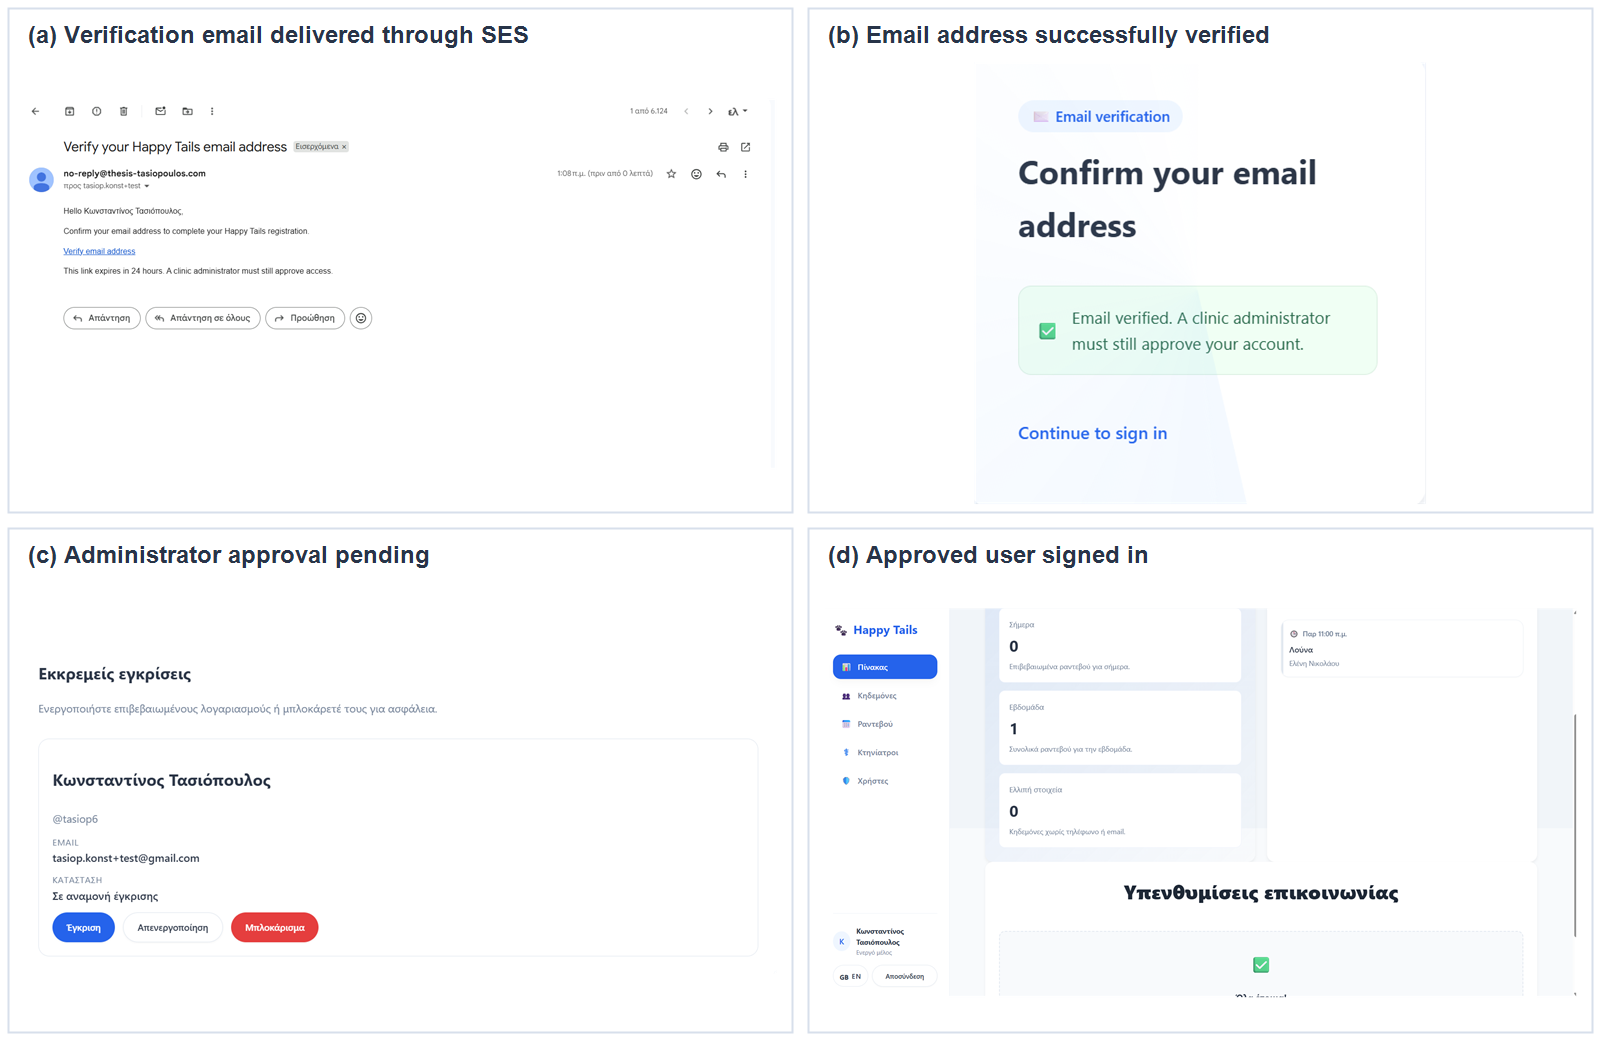
\includegraphics[width=\textwidth]{figures/application/registration-email-approval-flow.png}
\caption{End-to-end ροή νέου λογαριασμού: παράδοση verification email μέσω
SES, επιβεβαίωση διεύθυνσης, εκκρεμής έγκριση από administrator και επιτυχής
είσοδος του ενεργοποιημένου χρήστη.}
\label{fig:registration-email-approval-flow}
\end{figure}

Η ίδια υποδομή email αξιοποιήθηκε και για την ασφαλή επαναφορά κωδικού. Η
σελίδα εισόδου οδηγεί σε φόρμα όπου ζητείται μόνο η διεύθυνση email. Η
απόκριση παραμένει ίδια είτε υπάρχει ο λογαριασμός είτε όχι, ώστε να μην
αποκαλύπτεται σε τρίτους ποια email είναι καταχωρισμένα. Για υπαρκτό και
επαληθευμένο λογαριασμό δημιουργείται νέο τυχαίο token, αποθηκεύεται μόνο το
hash του και αποστέλλεται σύνδεσμος ισχύος 60 λεπτών. Η νέα τιμή του κωδικού
αποθηκεύεται με τον \texttt{PasswordEncoder} του Spring Security και το token
καταναλώνεται αμέσως, ώστε ο ίδιος σύνδεσμος να μην μπορεί να χρησιμοποιηθεί
δεύτερη φορά. Η υλοποίηση ελέγχθηκε με tests για έγκυρο, ληγμένο και κενό
token και στη συνέχεια με πραγματική αποστολή μέσω SES. Η
Εικόνα~\ref{fig:password-reset-flow} παρουσιάζει τα βασικά στάδια χωρίς να
εμφανίζει την τιμή του token.

\begin{figure}[htbp]
\centering
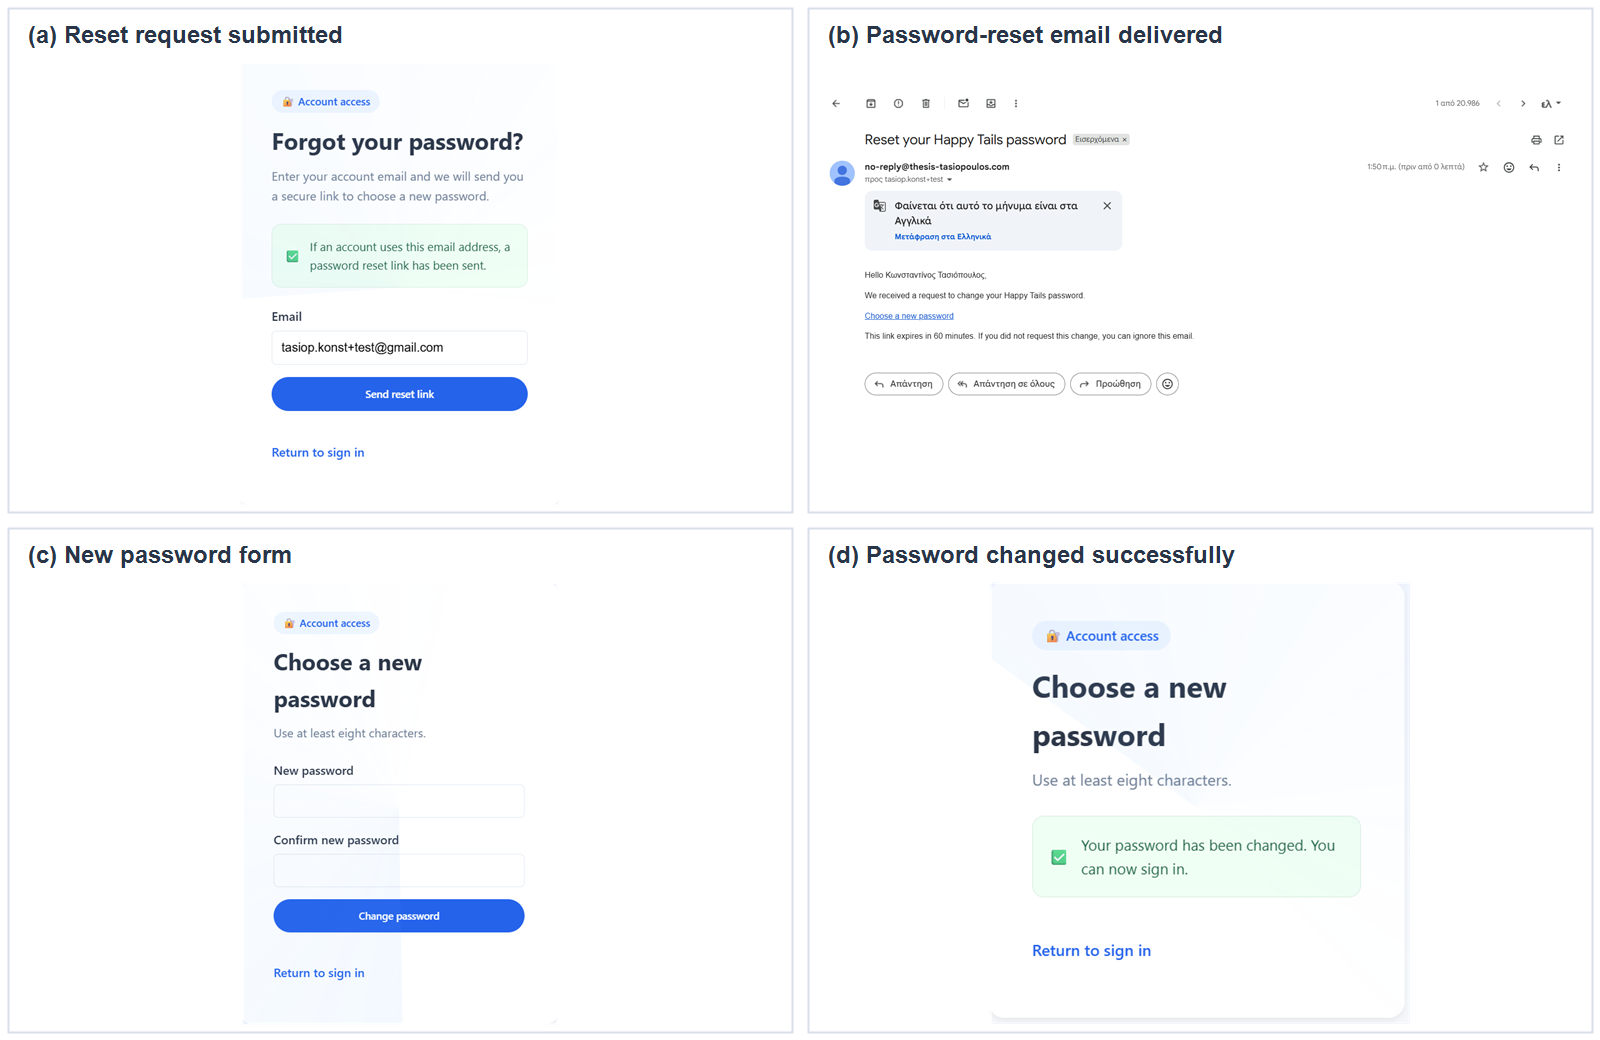
\includegraphics[width=\textwidth]{figures/application/password-reset-flow.png}
\caption{Ροή επαναφοράς κωδικού: ουδέτερη επιβεβαίωση του αιτήματος,
παράδοση email μέσω SES, εισαγωγή νέου κωδικού και επιτυχής ολοκλήρωση.}
\label{fig:password-reset-flow}
\end{figure}

\begin{figure}[htbp]
\centering
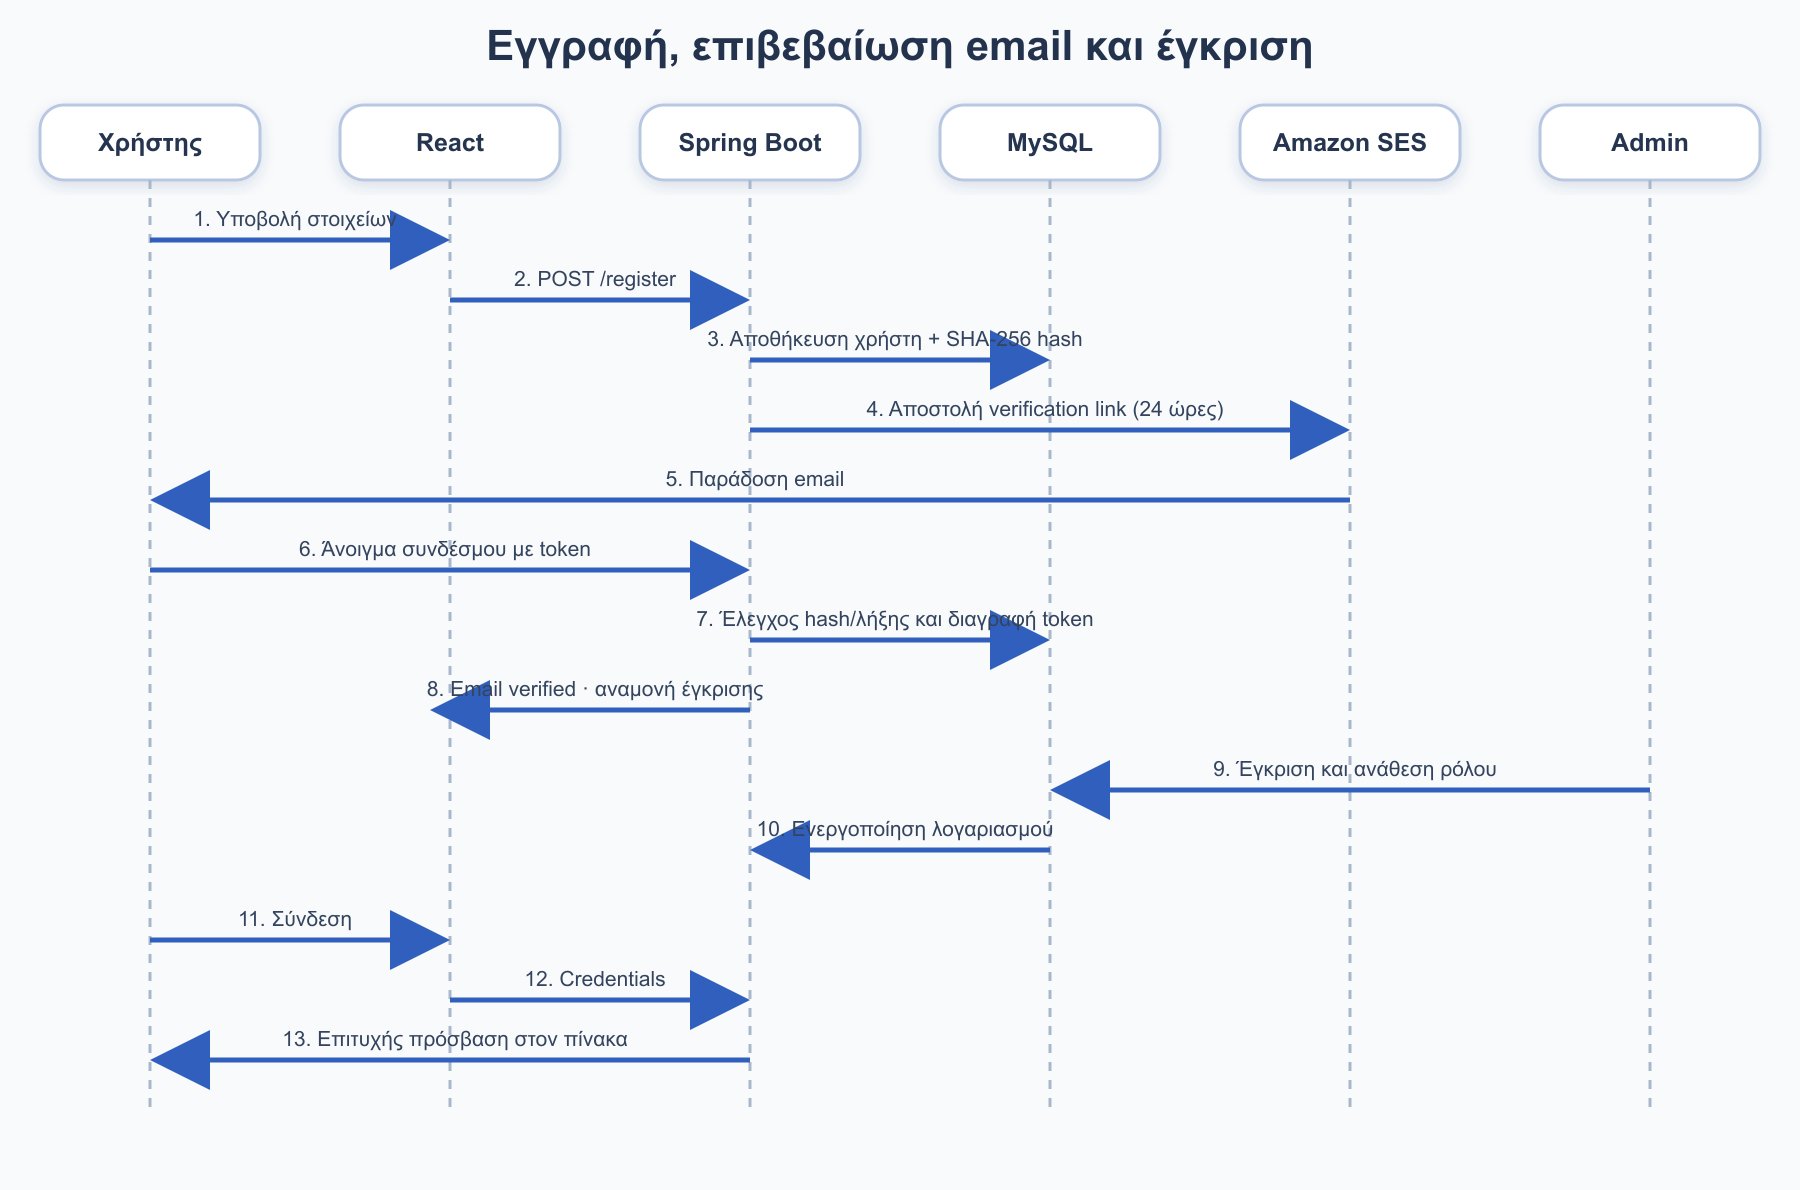
\includegraphics[width=\textwidth]{figures/application/registration-verification-sequence.png}
\caption{Ακολουθία εγγραφής, επιβεβαίωσης email και έγκρισης λογαριασμού.
Το token αποστέλλεται στον χρήστη, ενώ στη βάση αποθηκεύεται μόνο το hash
του. Η δυνατότητα σύνδεσης παρέχεται μετά την ανεξάρτητη έγκριση του
administrator.}
\label{fig:registration-verification-sequence}
\end{figure}

\section{Εγκατάσταση της εφαρμογής στην AWS}
Δημιουργήθηκε EC2 instance με Amazon Linux~2023, instance type
\texttt{t3.small}, EBS volume \texttt{gp3} 30~GiB και RSA key pair σε μορφή
OpenSSH. Κατά τη δημιουργία αντιστοιχίστηκε το security group της εφαρμογής
και, μετά την εκκίνηση, το instance έφθασε σε κατάσταση \texttt{Running} και
ολοκλήρωσε επιτυχώς τους ελέγχους κατάστασης της AWS. Η διαχειριστική σύνδεση
ελέγχθηκε μέσω SSH, ενώ η πρόσβαση στη θύρα 22 περιορίστηκε στην τρέχουσα
δημόσια IPv4 διεύθυνση του διαχειριστή με prefix \texttt{/32}. Η διεύθυνση
αυτή μπορεί να ενημερώνεται όταν μεταβάλλεται η σύνδεση του τοπικού δικτύου,
χωρίς να ανοίγει το SSH στο σύνολο του Internet.

Η διαδικασία δημιουργίας καταγράφηκε ως ακολουθία επαναλήψιμων βημάτων:
επιλογή Region και λειτουργικού συστήματος, διαμόρφωση compute και storage,
δημιουργία key pair και security group, εκκίνηση του instance, εγκατάσταση
του Docker runtime και ανάπτυξη των τριών containers.

\begin{figure}[htbp]
\centering
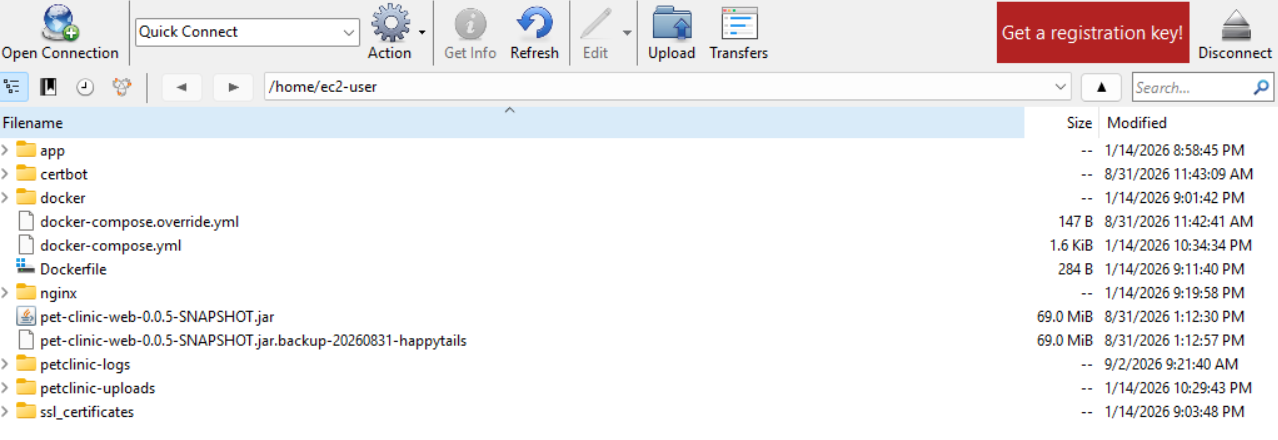
\includegraphics[width=0.95\textwidth]{figures/infrastructure/deployment-sftp-files.png}
\caption{Δομή των αρχείων deployment στο EC2 instance κατά την ασφαλή
διαχείριση μέσω SFTP. Διακρίνονται τα αρχεία Docker Compose, το application
JAR και οι κατάλογοι Nginx, πιστοποιητικών, logs και μεταφορτωμένων αρχείων.}
\label{fig:deployment-sftp-files}
\end{figure}

\begin{table}[htbp]
\caption{Έλεγχοι επαλήθευσης μετά τη δημιουργία της υποδομής και το deployment.}
\label{tab:deployment-verification}
\centering
\begin{tabularx}{\textwidth}{@{}p{4cm}p{3cm}X@{}}
\toprule
\textbf{Έλεγχος} & \textbf{Αναμενόμενο αποτέλεσμα} & \textbf{Καταγεγραμμένο αποτέλεσμα} \\
\midrule
EC2 status checks & 3/3 checks passed & Επιτυχής ολοκλήρωση και των τριών ελέγχων. \\
systemd failed units & Καμία αποτυχημένη μονάδα & Δεν εντοπίστηκαν failed units μετά την εκκίνηση. \\
Docker containers & Τρία containers σε λειτουργία & Spring Boot, MySQL και Nginx σε κατάσταση running. \\
MySQL health check & Healthy & Ο ενσωματωμένος health check ολοκληρώθηκε επιτυχώς. \\
Local HTTP request & HTTP 200 & Ο Nginx επέστρεψε επιτυχή απόκριση από το ίδιο το instance. \\
External DNS & Root και \texttt{www} στην Elastic IP & Και τα δύο ονόματα επιλύθηκαν στη \texttt{3.127.189.11}. \\
HTTP to HTTPS & HTTP 301 & Επιβεβαιώθηκε η μόνιμη ανακατεύθυνση. \\
HTTPS request & HTTP 200 και έγκυρο certificate & Επιβεβαιώθηκε εξωτερικά η ασφαλής πρόσβαση στην εφαρμογή. \\
\bottomrule
\end{tabularx}
\end{table}
\section{Παραμετροποίηση βάσης δεδομένων και μεταναστεύσεων}
Η MySQL~8.4 εκτελείται σε ανεξάρτητο container και δεν εκτίθεται ως δημόσια
υπηρεσία. Στο host η θύρα 3306 προσδένεται μόνο στη διεύθυνση
\texttt{127.0.0.1}, ενώ η εφαρμογή συνδέεται με το όνομα της υπηρεσίας
\texttt{petclinic-mysql} μέσω του εσωτερικού δικτύου Docker. Το όνομα της
βάσης και τα credentials παρέχονται από το αρχείο environment. Η MySQL
ρυθμίζεται με σύνολο χαρακτήρων \texttt{utf8mb4} και collation
\texttt{utf8mb4\_unicode\_ci}, ώστε να αποθηκεύονται χωρίς απώλεια ελληνικά
ονόματα και κείμενα.

Η διατήρηση των δεδομένων εξασφαλίζεται από το named volume
\texttt{mysql-data}, το οποίο προσαρτάται στο \texttt{/var/lib/mysql}. Έτσι,
η αντικατάσταση ή αναδημιουργία του container δεν συνεπάγεται διαγραφή των
δεδομένων. Ο ενσωματωμένος έλεγχος \texttt{mysqladmin ping} πρέπει να
ολοκληρωθεί επιτυχώς πριν ξεκινήσει η υπηρεσία Spring Boot. Η εξάρτηση αυτή
περιορίζει τις αποτυχημένες εκκινήσεις που θα προκαλούσε μία βάση η οποία
βρίσκεται ακόμη στο στάδιο αρχικοποίησης.

Η εξέλιξη του σχήματος καταγράφεται με Liquibase. Το κεντρικό αρχείο
\path{db.changelog-master.yaml} συμπεριλαμβάνει με σταθερή σειρά τα
changesets για τις σχέσεις ραντεβού, ιδιοκτήτη και κατοικίδιου, την
επιβεβαίωση email και τα tokens επαναφοράς κωδικού. Κατά την εκκίνηση, το
Liquibase συγκρίνει τα changesets με τους πίνακες
\path{DATABASECHANGELOG} και \path{DATABASECHANGELOGLOCK} και εφαρμόζει
μόνο όσα δεν έχουν ήδη εκτελεστεί. Με αυτόν τον τρόπο η ίδια έκδοση της
εφαρμογής μπορεί να αναπτυχθεί σε κενή ή υφιστάμενη βάση χωρίς χειροκίνητες
εντολές SQL.

Η ρύθμιση Hibernate DDL μπορεί να μεταβάλλεται μέσω environment variable.
Για αυστηρό production έλεγχο είναι προτιμότερη η τιμή
\texttt{validate}, ώστε το Hibernate να επιβεβαιώνει το σχήμα χωρίς να το
τροποποιεί και οι αλλαγές να παραμένουν αποκλειστική ευθύνη του Liquibase.
Η επαλήθευση πραγματοποιήθηκε με ελεγχόμενη επανεκκίνηση μόνο του Spring
container. Το Liquibase ανέγνωσε τον πίνακα \texttt{DATABASECHANGELOG},
ανέφερε τέσσερα changesets ως ήδη εκτελεσμένα, μηδενικές νέες εκτελέσεις και
επιτυχή αποδέσμευση του changelog lock. Συμπληρωματικό read-only ερώτημα στον
πίνακα επιβεβαίωσε τη σειρά και την κατάσταση \texttt{EXECUTED} και για τις
τέσσερις εγγραφές. Μετά την ολοκλήρωση, το container παρέμεινε σε κατάσταση
\texttt{Up} και η δημόσια διαδρομή επέστρεψε HTTPS~200. Η
Εικόνα~\ref{fig:liquibase-migrations} παρουσιάζει το σχετικό output χωρίς
credentials ή δεδομένα της εφαρμογής.

\begin{figure}[htbp]
\centering
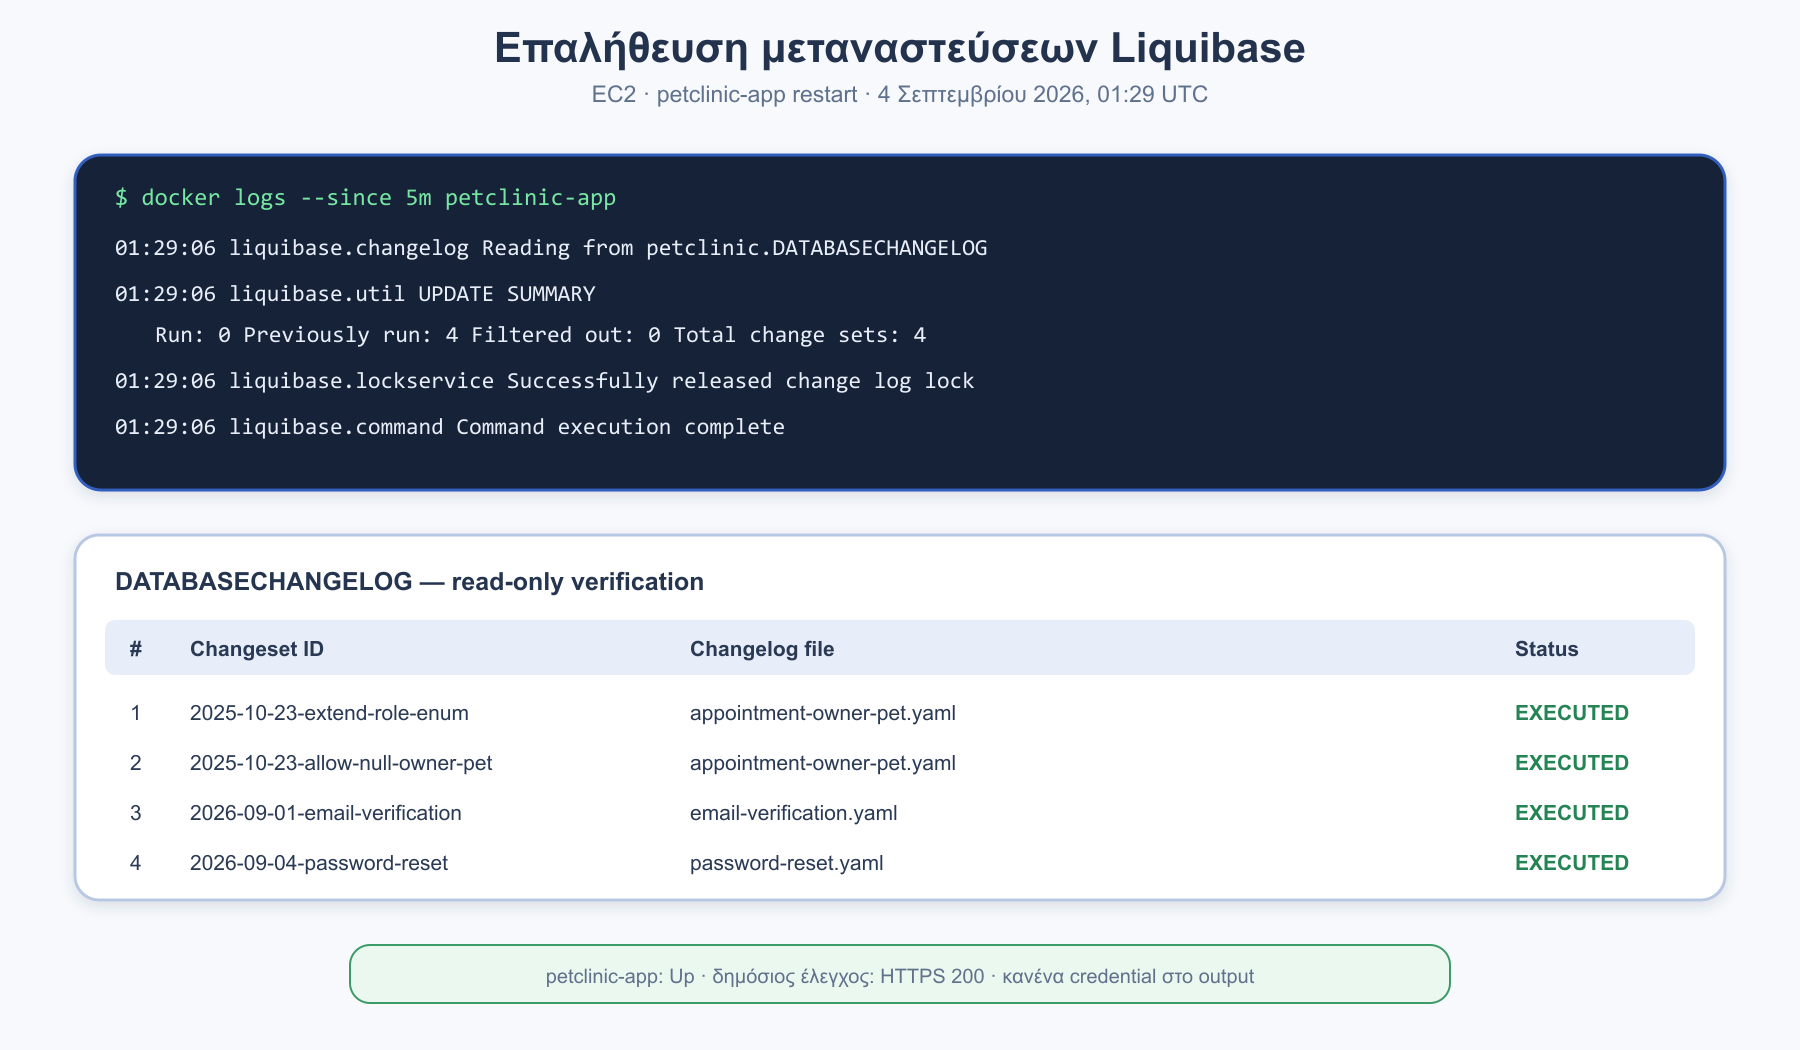
\includegraphics[width=\textwidth]{figures/infrastructure/liquibase-migrations.png}
\caption{Επαλήθευση Liquibase μετά από επανεκκίνηση του Spring container. Τα
startup logs δείχνουν ότι το schema ήταν ενημερωμένο, ενώ το read-only
ερώτημα στον πίνακα \texttt{DATABASECHANGELOG} επιβεβαιώνει τα τέσσερα
changesets που έχουν εφαρμοστεί.}
\label{fig:liquibase-migrations}
\end{figure}

\section{Διαχείριση στατικών και μεταφορτωμένων αρχείων}
Η παραγωγική έκδοση του React frontend δημιουργείται πριν από την παραγωγή
του Spring Boot JAR και διανέμεται μαζί με την εφαρμογή. Ο Nginx αποτελεί το
δημόσιο σημείο εισόδου και προωθεί τα αιτήματα στο backend, ενώ η ρύθμιση SPA
δρομολογεί τις client-side διαδρομές στο αρχικό έγγραφο της React. Με αυτόν
τον τρόπο δεν απαιτείται ξεχωριστός δημόσιος file server για τα στατικά
αρχεία της διεπαφής.

Τα έγγραφα του ιατρικού ιστορικού αποθηκεύονται από το
\path{DocumentStorageService} κάτω από τον κατάλογο
\path{/app/uploads/pet-documents}. Για κάθε κατοικίδιο δημιουργείται
ξεχωριστός υποκατάλογος και το φυσικό όνομα του αρχείου παράγεται από
timestamp και UUID. Η βάση δεδομένων διατηρεί τα μεταδεδομένα που χρειάζεται
η εφαρμογή, όπως το αρχικό όνομα, το content type, το μέγεθος και τη σχετική
διαδρομή. Ο διαχωρισμός αυτός επιτρέπει στη διεπαφή να εμφανίζει κατανοητό
όνομα χωρίς να χρησιμοποιεί το όνομα του χρήστη ως φυσικό όνομα αποθήκευσης.

Τόσο το Spring multipart configuration όσο και η υπηρεσία αποθήκευσης
επιβάλλουν μέγιστο μέγεθος 10~MB ανά αρχείο. Πριν από την ανάγνωση μιας
διαδρομής πραγματοποιούνται κανονικοποίηση και έλεγχος ότι το τελικό path
παραμένει εντός του ριζικού καταλόγου αποθήκευσης. Οι σχετικές unit tests
καλύπτουν σχετικές διαδρομές, διαχωριστικά Windows, αποθηκευμένες διαδρομές
με prefix, ανύπαρκτα αρχεία και απόρριψη αρχείου μεγαλύτερου από το όριο.

Ο κατάλογος \texttt{/app/uploads} προσαρτάται στο named volume
\texttt{petclinic-uploads}, ώστε τα έγγραφα να παραμένουν διαθέσιμα όταν
ανακατασκευάζεται μόνο το Spring container. Για τη λειτουργική επαλήθευση
μεταφορτώθηκε ένα τυχαίο PDF
έγγραφο, χωρίς συσχέτιση με πραγματικό ιατρικό περιστατικό. Η εφαρμογή το
κατέγραψε ως \texttt{application/pdf}, μεγέθους περίπου 1,1~MB, και το
εμφάνισε στη σχετική καρτέλα, όπως φαίνεται στην
Εικόνα~\ref{fig:uploaded-document-record}. Το πλήκτρο \enquote{Προβολή}
ανακτά επιτυχώς το αποθηκευμένο αρχείο και εμφανίζει το PDF στον browser,
επιβεβαιώνοντας και τη διαδρομή ανάγνωσης του συνημμένου. Το περιεχόμενο του
τυχαίου παραστατικού δεν συμπεριλαμβάνεται στην τεκμηρίωση, καθώς δεν αποτελεί
ιατρικό δεδομένο ούτε απαιτείται για την απόδειξη της λειτουργίας.

\begin{figure}[htbp]
\centering
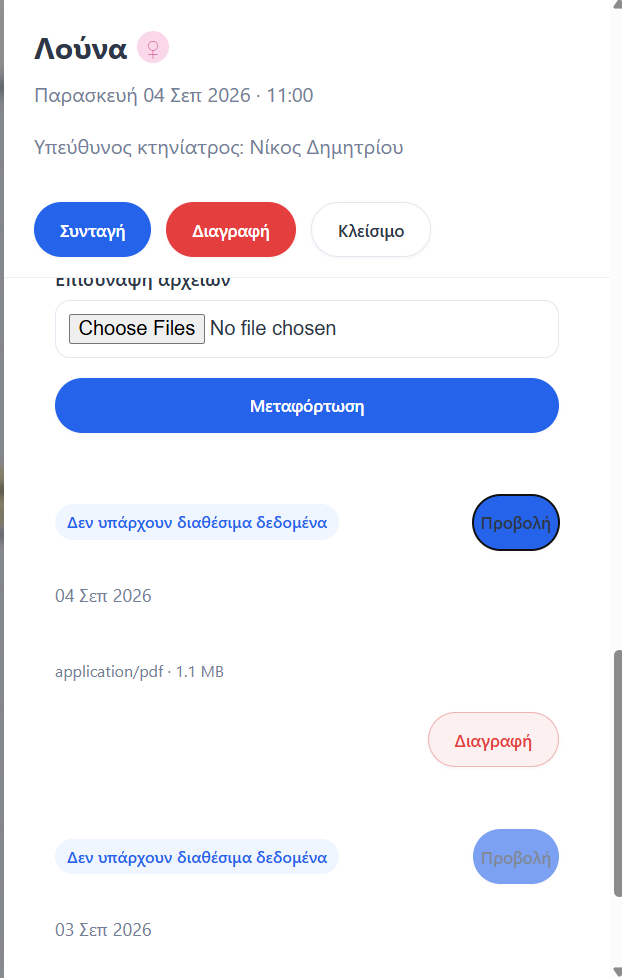
\includegraphics[width=0.46\textwidth]{figures/application/uploaded-document-record.png}
\caption{Επιτυχής αποθήκευση δοκιμαστικού PDF ως συνημμένου σε εγγραφή της
εφαρμογής. Διακρίνονται ο τύπος, το μέγεθος και το ενεργό πλήκτρο
\enquote{Προβολή}, μέσω του οποίου επαληθεύτηκε η επιτυχής ανάκτηση και
εμφάνιση του PDF, χωρίς να δημοσιοποιείται το περιεχόμενό του.}
\label{fig:uploaded-document-record}
\end{figure}

Πριν από την επανεκκίνηση καταγράφηκαν η παραγόμενη διαδρομή, το ακριβές
μέγεθος των 1.191.697 bytes και το SHA-256 checksum του αρχείου. Μετά από
επανεκκίνηση αποκλειστικά του \texttt{petclinic-app}, η ίδια διαδρομή
παρέμεινε διαθέσιμη με αμετάβλητο μέγεθος και checksum, ενώ η δημόσια
διαδρομή της εφαρμογής επέστρεψε HTTPS~200. Το αποτέλεσμα επιβεβαιώνει ότι το
αρχείο βρίσκεται στο persistent volume και όχι στο προσωρινό writable layer
του container. Η συγκεντρωτική απεικόνιση της δοκιμής έχει προετοιμαστεί για
την αξιολόγηση αξιοπιστίας του Κεφαλαίου~6.

\section{Ρύθμιση DNS, HTTPS και αντίστροφου διακομιστή μεσολάβησης}
Ο Nginx προωθεί τα αιτήματα προς την υπηρεσία Spring Boot στη θύρα 8080 του
εσωτερικού δικτύου Docker και διατηρεί τις επικεφαλίδες
\texttt{X-Real-IP}, \texttt{X-Forwarded-For} και
\texttt{X-Forwarded-Proto}. Η δημόσια πρόσβαση γίνεται μέσω των εγγραφών
Route~53 και της σταθερής Elastic IP. Για την έκδοση του πιστοποιητικού
χρησιμοποιήθηκε η μέθοδος HTTP-01 του Let's Encrypt για τα δύο δημόσια
ονόματα. Ο Nginx ρυθμίστηκε για TLS~1.2 και TLS~1.3 και επιστρέφει ανακατεύθυνση
301 από HTTP προς HTTPS. Η ανανέωση εκτελείται καθημερινά από χρονοδιακόπτη
systemd, ο οποίος εκκινεί προσωρινό container Certbot και στη συνέχεια
επαναφορτώνει τη ρύθμιση του Nginx. Μετά τη ρύθμιση επαληθεύτηκαν η ορθότητα
του αρχείου Nginx, απόκριση HTTPS~200 και η κανονική προβολή της εφαρμογής.

\begin{figure}[htbp]
\centering
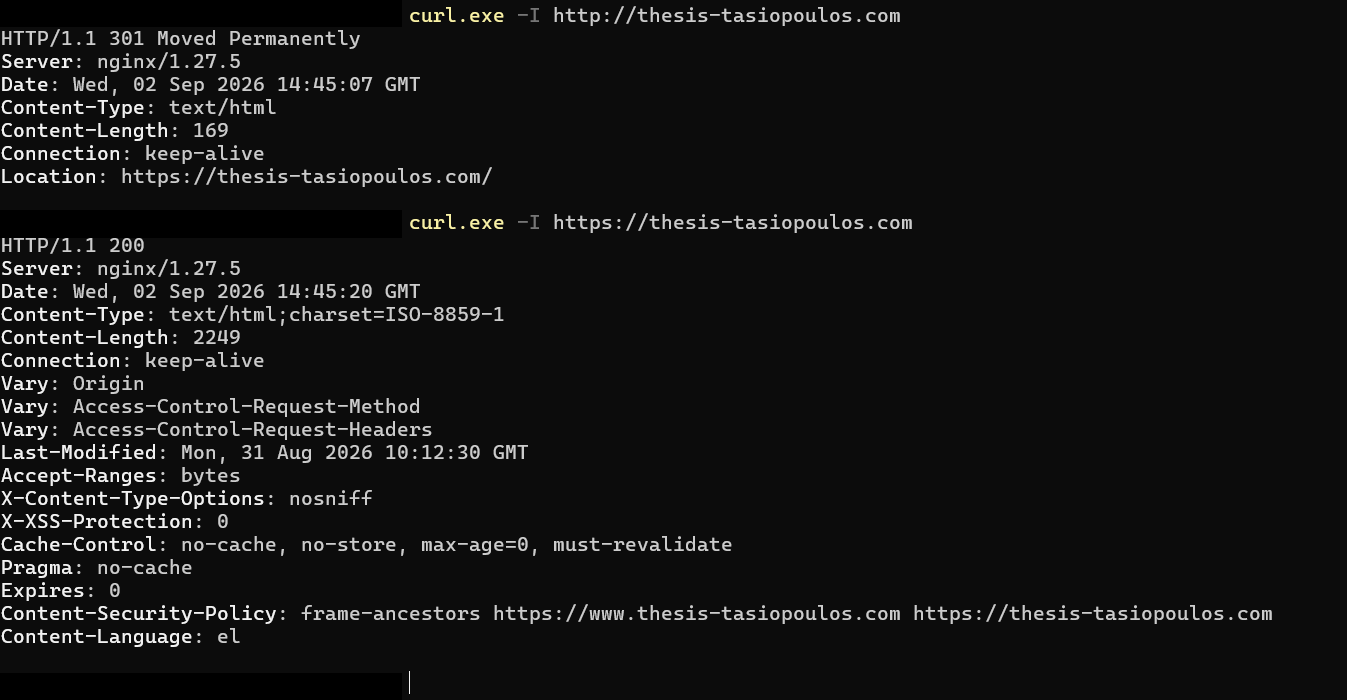
\includegraphics[width=0.96\textwidth]{figures/infrastructure/http-https-verification.png}
\caption{Εξωτερικός έλεγχος της δημόσιας πρόσβασης: το HTTP endpoint
επιστρέφει μόνιμη ανακατεύθυνση 301 προς HTTPS, ενώ το HTTPS endpoint
επιστρέφει επιτυχή απόκριση 200. Η τοπική διαδρομή χρήστη έχει αποκρυφθεί.}
\label{fig:http-https-verification}
\end{figure}
\section{Παρακολούθηση λειτουργίας και αντίγραφα ασφαλείας}
Η αρχική επαλήθευση περιέλαβε τους ελέγχους κατάστασης EC2, την κατάσταση
υγείας του container της MySQL, την κατάσταση των τριών containers και
αίτημα HTTP προς τον Nginx. Η εφαρμογή επέστρεψε κωδικό 200 και η αρχική
ελληνική σελίδα προβλήθηκε επιτυχώς σε εξωτερικό πρόγραμμα περιήγησης. Η
τελική αξιολόγηση συμπληρώθηκε με βασικά EC2 metrics και status checks από
το CloudWatch, έλεγχο των πραγματικών παραγόντων κόστους και καταγραφή της
συμπεριφοράς της εγκατάστασης κατά την επανεκκίνηση. Τα αντίστοιχα
αποτελέσματα, οι χρονικές περίοδοι μέτρησης και οι περιορισμοί παρουσιάζονται
αναλυτικά στο Κεφάλαιο~6. Η δοκιμή επιβεβαίωσε τη διατήρηση δεδομένων στο
υπάρχον instance, όχι όμως πλήρες restore από snapshot σε νέο περιβάλλον.
\section{Διαδικασία ενημέρωσης και επανεκκίνησης}
Η ενημέρωση της εφαρμογής περιλαμβάνει παραγωγή νέου JAR, μεταφορά του στο
instance, rebuild του Spring container και ελέγχους λειτουργίας, χωρίς να
απαιτείται αναδημιουργία της MySQL ή του Nginx. Η διαδικασία ενημέρωσης έχει
ήδη εφαρμοστεί σε αλλαγές της δημόσιας διεπαφής. Ο ελεγχόμενος reboot του
instance εκτελέστηκε ως χωριστό πείραμα. Καταγράφηκε ο χρόνος μέχρι την
επιστροφή της δημόσιας υπηρεσίας και επιβεβαιώθηκαν η αυτόματη εκκίνηση του
Docker, η προσάρτηση των persistent volumes και η κατάσταση των containers.
Το endpoint επανήλθε σε 40,79~s χωρίς απώλεια των ελεγχόμενων δεδομένων, όπως
τεκμηριώνεται στην Ενότητα~6.6.

\begin{figure}[htbp]
\centering
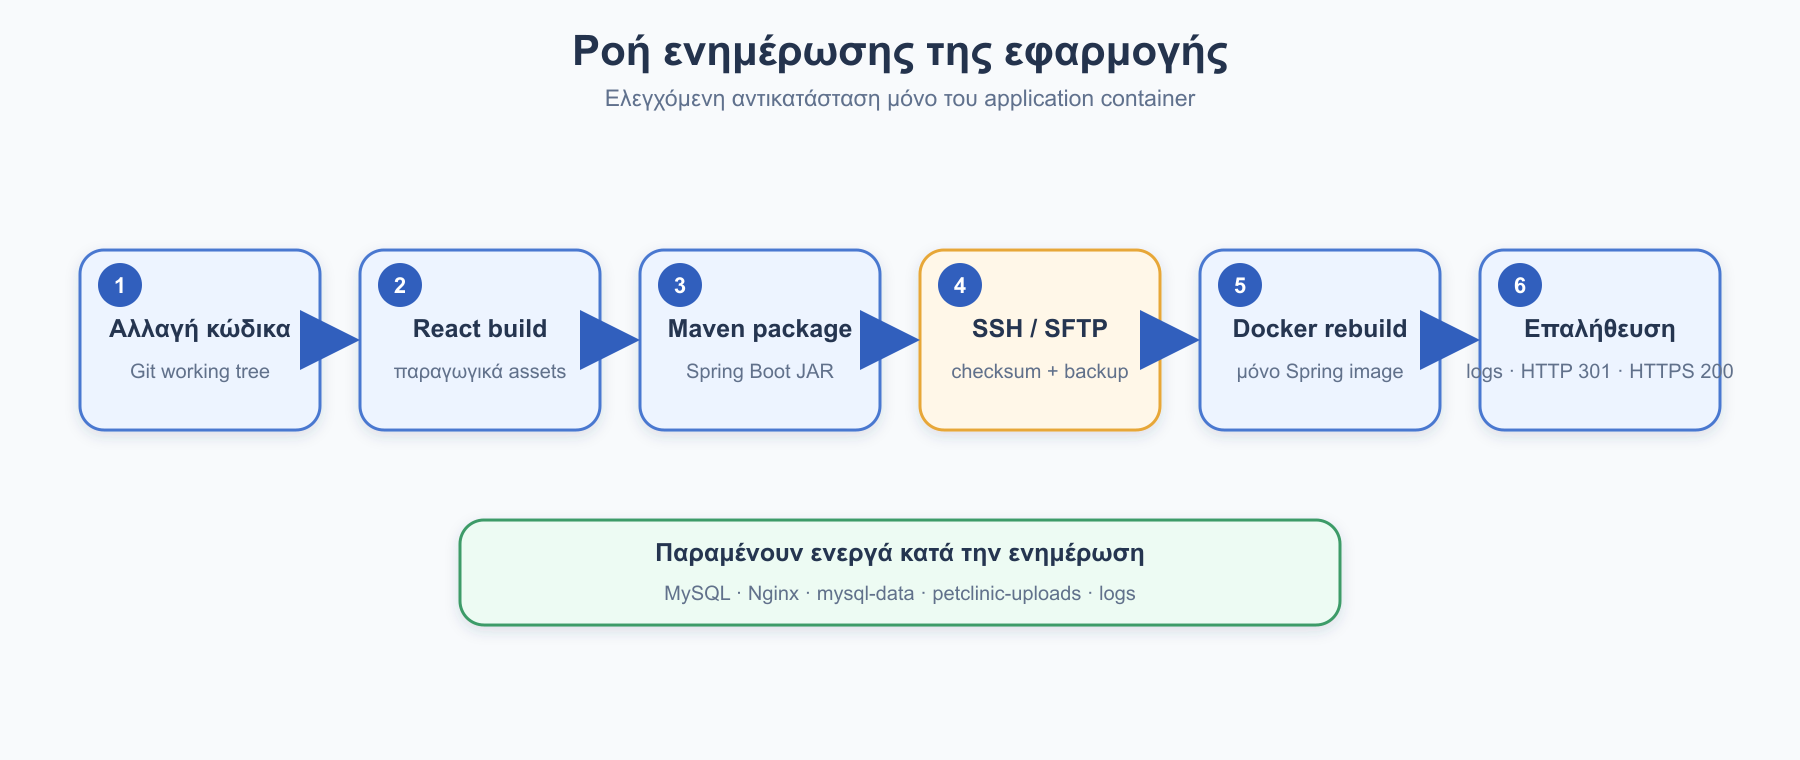
\includegraphics[width=\textwidth]{figures/infrastructure/deployment-pipeline.png}
\caption{Ροή ενημέρωσης και επαλήθευσης του application deployment. Κατά
την ανανέωση ανακατασκευάζεται μόνο το Spring image, ενώ η MySQL, ο Nginx και
τα persistent volumes παραμένουν ενεργά.}
\label{fig:deployment-pipeline}
\end{figure}



\chapter{Πειραματική Αξιολόγηση}
\section{Μεθοδολογία και περιβάλλον πειραμάτων}
Η αξιολόγηση οργανώθηκε ώστε κάθε συμπέρασμα να συνδέεται με συγκεκριμένη
μέτρηση ή λειτουργικό τεκμήριο. Ως περιβάλλον
αναφοράς χρησιμοποιείται EC2 instance τύπου \texttt{t3.small} στην περιοχή
\texttt{eu-central-1}, με Amazon Linux~2023 και EBS volume \texttt{gp3}
30~GiB. Στο instance εκτελούνται τρία Docker containers: Nginx, Spring Boot
και MySQL~8.4. Το Nginx αποτελεί το μοναδικό δημόσιο σημείο εισόδου στις
θύρες 80 και 443, ενώ η βάση δεδομένων παραμένει στο εσωτερικό δίκτυο της
εγκατάστασης.

Για να είναι συγκρίσιμα τα πειράματα, κάθε βαθμίδα φόρτου χρησιμοποίησε την
ίδια έκδοση εφαρμογής, σταθερό συνθετικό σύνολο δεδομένων και κοινή αρχική
κατάσταση. Οι χρόνοι καταγράφηκαν σε UTC και τα αποτελέσματα εφαρμογής
συσχετίστηκαν με τα metrics του ίδιου χρονικού παραθύρου στο CloudWatch.
Η Εικόνα~\ref{fig:experimental-workflow} συνοψίζει τη διαδικασία.

\begin{figure}[htbp]
\centering
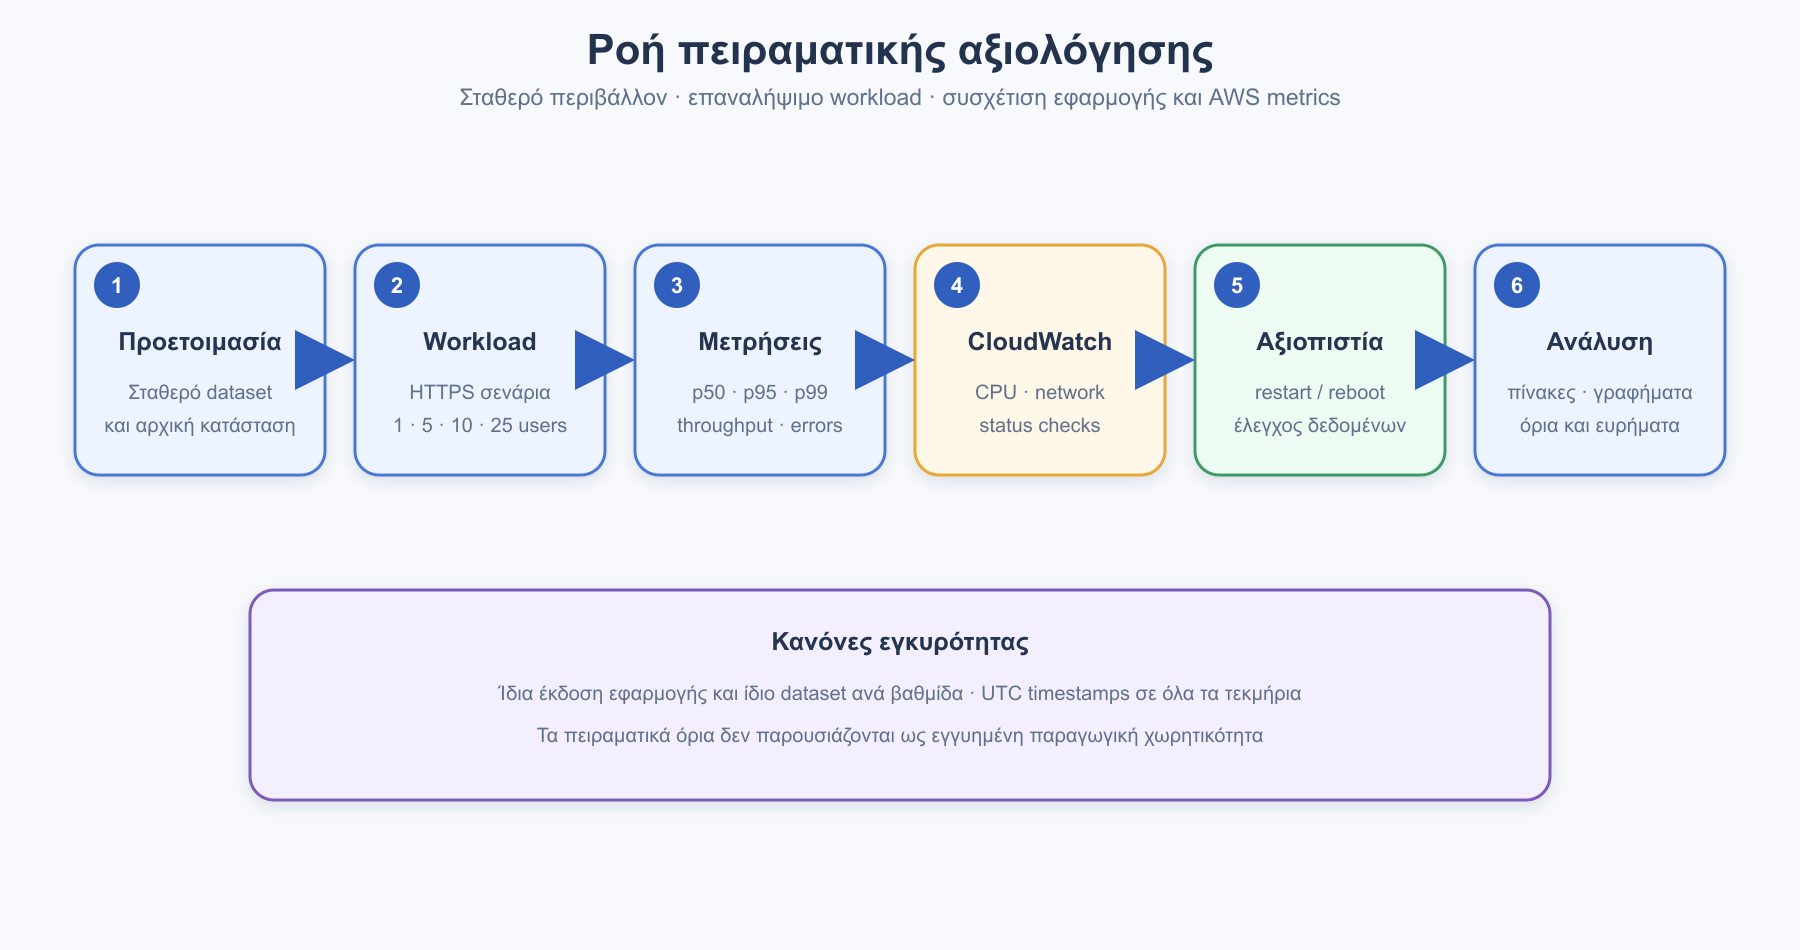
\includegraphics[width=\textwidth]{figures/evaluation/experimental-workflow.png}
\caption{Ροή πειραματικής αξιολόγησης από την προετοιμασία του σταθερού
dataset έως τη συσχέτιση των χρόνων απόκρισης, των AWS metrics και των
ελέγχων αξιοπιστίας.}
\label{fig:experimental-workflow}
\end{figure}

Οι μεταβλητές που καταγράφηκαν είναι ο αριθμός αιτημάτων, το throughput
(ρυθμός ολοκλήρωσης επιτυχών αιτημάτων ανά δευτερόλεπτο), το ποσοστό
σφαλμάτων, οι χρόνοι απόκρισης p50, p95 και p99, καθώς και CPU, network
traffic και status checks του EC2. Τα p50, p95 και p99 είναι εκατοστημόρια
(percentiles) και όχι ποσοστά καθυστέρησης: p50 είναι η διάμεσος, ενώ p95
σημαίνει ότι το 95\% των αποκρίσεων ολοκληρώθηκε σε χρόνο μικρότερο ή ίσο
από την αναφερόμενη τιμή και το βραδύτερο 5\% χρειάστηκε περισσότερο χρόνο.
Αντίστοιχα, το p99 καλύπτει το 99\% και απομονώνει το βραδύτερο 1\% των
παρατηρήσεων. Τα εκατοστημόρια είναι χρησιμότερα από έναν μεμονωμένο μέσο
όρο όταν λίγες πολύ αργές αποκρίσεις δημιουργούν ουρά καθυστέρησης
\cite{grafana2026k6metrics,grafana2026k6thresholds}.

Η μνήμη του application container καταγράφηκε με στιγμιότυπα του Docker και
όχι ως βασικό EC2 metric, επειδή δεν είχε εγκατασταθεί CloudWatch Agent.
Κάθε αριθμητικό αποτέλεσμα συνοδεύεται από διάρκεια, βαθμίδα ταυτόχρονων
χρηστών και ακριβές χρονικό παράθυρο.

\section{Λειτουργική επαλήθευση}
Οι λειτουργικοί έλεγχοι πραγματοποιήθηκαν στην παραγωγική εγκατάσταση με
συνθετικά δεδομένα. Μετά την ενεργοποίηση του Docker, τα containers της
εφαρμογής και του Nginx βρέθηκαν σε κατάσταση λειτουργίας, ενώ η MySQL πέρασε
τον ενσωματωμένο έλεγχο υγείας. Τα root και \texttt{www} DNS names επιλύθηκαν
στην ίδια Elastic IP, η διαδρομή HTTP επέστρεψε μόνιμη ανακατεύθυνση 301 και
η τελική διαδρομή HTTPS επέστρεψε 200 με έγκυρο πιστοποιητικό.

Η ροή νέου λογαριασμού επαληθεύτηκε από άκρο σε άκρο: υποβολή εγγραφής,
παράδοση email μέσω Amazon SES, επιβεβαίωση διεύθυνσης, απόρριψη σύνδεσης όσο
ο λογαριασμός παρέμενε ανενεργός, έγκριση από administrator και επιτυχής
είσοδος. Με την ίδια υποδομή email επαληθεύτηκε η αίτηση επαναφοράς κωδικού,
η παραλαβή συνδέσμου, η επιλογή νέου κωδικού και η επιτυχής μεταγενέστερη
σύνδεση.

Ελέγχθηκε επίσης η ασφαλής διαγραφή λογαριασμών προσωπικού. Τέσσερα
αυτοματοποιημένα tests επιβεβαίωσαν τη διαγραφή απλού προσωπικού και ιδιοκτήτη
κλινικής χωρίς ραντεβού, την προστασία του \texttt{SUPERADMIN} και την
απόρριψη με HTTP~409 όταν υπάρχουν συνδεδεμένες εγγραφές ραντεβού.

Η production σελίδα \enquote{Profile \& Integrations} επαληθεύτηκε επίσης
ως προσβάσιμη τόσο από τη διαδρομή \texttt{/profile} όσο και από την κάρτα
του συνδεδεμένου χρήστη στην πλευρική πλοήγηση. Εμφάνισε ανεξάρτητα τα
στοιχεία επικοινωνίας και την κατάσταση Google Calendar, ενώ η επιλογή
\enquote{Connect Google Calendar} οδήγησε επιτυχώς στην πραγματική οθόνη
συγκατάθεσης της Google για τον μοναδικό OAuth test user. Κατά την πρώτη
δοκιμή εντοπίστηκε αστοχία στη διαδρομή επιστροφής: ένα παρωχημένο ή
αντικατεστημένο \texttt{state} παρήγαγε \texttt{reason=invalid} και η σελίδα
αποτελέσματος προστατευόταν λανθασμένα, με συνέπεια HTTP~401. Η διόρθωση
κατέστησε δημόσια μόνο τη σελίδα αποτελέσματος, διατήρησε προστατευμένο το
profile, όρισε ρητά ασφαλή χαρακτηριστικά στο session cookie και πρόσθεσε
καταγραφή των αποτυχιών ελέγχου \texttt{state}. Η διόρθωση αναπτύχθηκε στην
παραγωγή και επαληθεύτηκε με επιτυχή εκκίνηση του Spring container, παρουσία
των μεταβλητών Google και απόκριση HTTPS~200. Η διαδρομή αποτελέσματος
ελέγχθηκε επίσης άμεσα και επέστρεψε HTTP~200 αντί του προηγούμενου 401. Η
εξουσιοδότηση του λογαριασμού administrator ολοκληρώθηκε και δύο υπάρχοντα
ραντεβού δημιουργήθηκαν στο Google Calendar. Η πρώτη οπτική σύγκριση ανέδειξε
μετατόπιση τριών ωρών: ώρες 11:00 και 12:00 της εφαρμογής εμφανίστηκαν ως
14:00 και 15:00, επειδή το container χρησιμοποιούσε UTC για τοπικές τιμές.
Η μετατροπή διορθώθηκε ώστε να χρησιμοποιεί ρητά τη ζώνη
\texttt{Europe/Athens} και αναπτύχθηκε εκ νέου στην παραγωγή. Στην επανάληψη
του ελέγχου, το ενημερωμένο ραντεβού εμφανίστηκε στις 09:30 τόσο στο Happy
Tails όσο και στο Google Calendar, ενώ η πρόσκληση email ανέφερε 09:30--10:00
και Eastern European Time--Athens. Η διαγραφή αφαίρεσε το απομακρυσμένο event
και το Google Calendar παρήγαγε την αντίστοιχη ειδοποίηση ακύρωσης. Το
συγκεκριμένο τεκμήριο αφορά το κανάλι Google και όχι μήνυμα από τον
\texttt{no-reply} sender του Amazon SES. Έτσι επαληθεύτηκαν οι ροές create, update
και delete μαζί με τη σωστή μετατροπή ζώνης ώρας.
Στο συγκεκριμένο test ο administrator/organizer και η client owner
χρησιμοποίησαν διαφορετικές διευθύνσεις και ανεξάρτητες θυρίδες email.
Επομένως επαληθεύτηκε τόσο η παραγωγή των role-based παραληπτών όσο και η
παράδοση της πρόσκλησης σε διακριτό παραλήπτη ιδιοκτήτη.

Στον ιατρικό φάκελο μεταφορτώθηκε τυχαίο PDF, μη συνδεδεμένο με πραγματικό
περιστατικό. Η εφαρμογή αποθήκευσε τα metadata και εμφάνισε ενεργή ενέργεια
\enquote{Προβολή}. Η επιλογή της ενέργειας ανέκτησε και εμφάνισε επιτυχώς το
PDF στον browser. Το περιεχόμενο του παραστατικού δεν χρησιμοποιείται ως
δεδομένο της μελέτης και δεν παρουσιάζεται στη διατριβή.

\begin{table}[htbp]
\centering
\caption{Συνοπτικά αποτελέσματα λειτουργικής επαλήθευσης.}
\label{tab:functional-verification}
\small
\begin{tabularx}{\textwidth}{p{0.28\textwidth}X p{0.18\textwidth}}
\toprule
Έλεγχος & Παρατηρηθέν αποτέλεσμα & Κατάσταση \\
\midrule
Docker services & Spring Boot και Nginx σε λειτουργία, MySQL healthy & Επιτυχία \\
DNS και TLS & Root/\texttt{www} στην Elastic IP, HTTP 301, HTTPS 200 & Επιτυχία \\
Εγγραφή χρήστη & SES email, verification, διοικητική έγκριση, login & Επιτυχία \\
Επαναφορά κωδικού & Email reset, αλλαγή κωδικού και νέα είσοδος & Επιτυχία \\
Διαγραφή λογαριασμού προσωπικού & Επιτυχία για μη χρησιμοποιούμενο λογαριασμό, προστασία \texttt{SUPERADMIN} και HTTP~409 όταν υπάρχουν ραντεβού & Επιτυχία \\
Μεταφόρτωση PDF & Αποθήκευση metadata και αρχείου περίπου 1,1~MB & Επιτυχία \\
Προβολή PDF & Ανάκτηση και εμφάνιση μέσω \enquote{Προβολή} & Επιτυχία \\
Liquibase startup & 4 previously run, 0 νέα changesets, lock released & Επιτυχία \\
Profile και OAuth consent & Πρόσβαση από user card, συγκατάθεση και σύνδεση administrator Calendar & Επιτυχία \\
Google event create/update & Ίδιο event στις 09:30 σε εφαρμογή, Google Calendar και πρόσκληση Athens & Επιτυχία \\
Google event delete & Αφαίρεση απομακρυσμένου event και παραλαβή ειδοποίησης ακύρωσης & Επιτυχία \\
\bottomrule
\end{tabularx}
\end{table}

\section{Περιορισμένο proof of concept με Amazon CloudFront}
Δημιουργήθηκε ξεχωριστή CloudFront distribution με όνομα
\path{happy-tails-thesis-poc}, σύμφωνα με τις παραμέτρους διανομής που
τεκμηριώνει η AWS~\cite{aws2026cloudfront}. Ως custom origin ορίστηκε το
υφιστάμενο HTTPS endpoint \texttt{thesis-tasiopoulos.com}. Δεν ορίστηκε
alternate domain name και δεν τροποποιήθηκαν οι εγγραφές Route~53· επομένως
η παραγωγική διαδρομή παρέμεινε ανεξάρτητη από το πείραμα. Η πρόσβαση στη
δοκιμή έγινε αποκλειστικά από το προεπιλεγμένο hostname
\path{dkaqy32zt0b9h.cloudfront.net}.

Επειδή η εφαρμογή είναι δυναμική και χρησιμοποιεί authenticated API calls,
η προεπιλεγμένη συμπεριφορά ρυθμίστηκε με \texttt{CachingDisabled}, με
origin request policy \path{AllViewerExceptHostHeader}. Με αυτόν τον τρόπο
προωθούνται cookies, query strings και viewer headers, αλλά το \texttt{Host}
προσαρμόζεται στο origin ώστε να συμφωνεί με το πιστοποιητικό TLS του
\texttt{thesis-tasiopoulos.com}. Επιτράπηκαν οι μέθοδοι \texttt{GET},
\texttt{HEAD}, \texttt{OPTIONS}, \texttt{PUT}, \texttt{POST}, \texttt{PATCH}
και \texttt{DELETE}, ενώ τόσο η σύνδεση viewer--CloudFront όσο και η σύνδεση
CloudFront--origin προστατεύονται με HTTPS. Οι ενσωματωμένες προστασίες WAF
του plan ενεργοποιήθηκαν σε monitor mode, ώστε το πείραμα να παρατηρεί
αιτήματα χωρίς να παρεμβαίνει στη λειτουργία τους.

Η λειτουργική επαλήθευση έδειξε ότι η δημόσια αρχική σελίδα και η διαδρομή
\texttt{/login} φορτώθηκαν επιτυχώς μέσω του CloudFront hostname. Επιπλέον,
αίτημα προς την HTTP εκδοχή του hostname ανακατευθύνθηκε αυτόματα σε HTTPS.
Οι έλεγχοι αυτοί τεκμηριώνουν τη βασική συνδεσιμότητα και τη δρομολόγηση, όχι
όμως βελτίωση απόδοσης, διότι το caching παρέμεινε σκόπιμα απενεργοποιημένο
και δεν έχει ακόμη εκτελεστεί συγκριτικό workload.

\section{Αξιολόγηση απόδοσης και χρόνου απόκρισης}
Η αρχική μέτρηση χρόνου απόκρισης κάλυψε τόσο τη δημόσια αρχική σελίδα όσο
και αυθεντικοποιημένες λειτουργίες. Πριν από τη μέτρηση αναπτύχθηκε και
επαληθεύτηκε πανομοιότυπο artifact με SHA-256
\texttt{317132aeac05\ldots 2153c82f3}. Χρησιμοποιήθηκε απομονωμένος
συνθετικός λογαριασμός με αποκλειστικά τον ρόλο \texttt{STAFF}, χωρίς
συσχέτιση με πραγματικό πρόσωπο, κτηνίατρο, Google Calendar ή πραγματική
διεύθυνση email. Ο κωδικός δημιουργήθηκε τυχαία για το πείραμα και δεν
καταγράφηκε στο αποτέλεσμα.

Μετά από πέντε αιτήματα warm-up, δηλαδή προκαταρκτικά αιτήματα για την
αρχικοποίηση συνδέσεων και runtime paths πριν από τη μέτρηση, ένας εικονικός
χρήστης (Virtual User, VU) πραγματοποίησε για
60,04~s κυκλικά αιτήματα προς τη δημόσια αρχική σελίδα και τα
\texttt{GET /api/dashboard}, \texttt{GET /api/owners} και
\texttt{GET /api/appointments}. Η αυθεντικοποίηση εκτελέστηκε μία φορά στην
αρχή μέσω \texttt{POST /api/auth/login}. Το ακριβές παράθυρο ήταν
2026-09-05 13:19:08,191 έως 13:20:08,220~UTC. Καταγράφηκαν 895 αιτήματα με
895 επιτυχίες, μηδενικά σφάλματα και συνολικό throughput 14,91
αιτήματα/s. Τα αποτελέσματα ανά endpoint παρουσιάζονται στον
Πίνακα~\ref{tab:baseline-response-times}.

\begin{table}[htbp]
\centering
\caption{Χρόνοι απόκρισης του baseline με έναν εικονικό χρήστη.}
\label{tab:baseline-response-times}
\small
\setlength{\tabcolsep}{4pt}
\begin{tabularx}{\textwidth}{>{\raggedright\arraybackslash}X r r r r r}
\toprule
Endpoint & Αιτήματα & p50 (ms) & p95 (ms) & p99 (ms) & Σφάλματα \\
\midrule
\path{POST /api/auth/login} & 1 & 429,53 & 429,53 & 429,53 & 0 \\
\texttt{GET /} & 223 & 59,97 & 67,87 & 355,49 & 0 \\
\path{GET /api/dashboard} & 224 & 58,06 & 83,35 & 141,20 & 0 \\
\path{GET /api/owners} & 224 & 69,19 & 91,85 & 108,70 & 0 \\
\path{GET /api/appointments} & 223 & 64,03 & 77,20 & 93,66 & 0 \\
\bottomrule
\end{tabularx}
\end{table}

Η μοναδική μέτρηση login δεν αποτελεί κατανομή και παρατίθεται μόνο ως
χρόνος αρχικοποίησης. Στα επαναλαμβανόμενα endpoints, το υψηλότερο p95 ήταν
91,85~ms στη λίστα ιδιοκτητών. Το p99 της αρχικής σελίδας έφθασε τα
355,49~ms, παρότι το p95 παρέμεινε 67,87~ms, γεγονός που δείχνει λίγες
μεμονωμένες αργές αποκρίσεις και δικαιολογεί τη χρήση percentiles αντί ενός
μόνο μέσου όρου. Δεν καταγράφηκαν \texttt{ERROR}, exception ή
\texttt{OutOfMemory} μηνύματα στο Spring container κατά το ίδιο παράθυρο,
ενώ ο έλεγχος μετά τη δοκιμή επέστρεψε HTTPS~200.

Τα βασικά EC2 metrics του CloudWatch συσχετίστηκαν με τα δύο πεντάλεπτα
διαστήματα που τέμνουν το workload. Στο διάστημα 13:15--13:20~UTC η μέση και
μέγιστη CPU ήταν 3,10\% και 10,20\%, με 335.554 bytes εισόδου και 1.080.736
bytes εξόδου. Στο διάστημα 13:20--13:25~UTC οι διαθέσιμες κατά τη συλλογή
τιμές ήταν 8,85\% μέση και 16,25\% μέγιστη CPU, 102.778 bytes εισόδου και
311.303 bytes εξόδου. Το \texttt{StatusCheckFailed} ήταν μηδέν και στα δύο
διαστήματα. Επειδή η δοκιμή διήρκεσε ένα λεπτό και διέσχισε το όριο των
13:20, τα πεντάλεπτα metrics αποτελούν συσχετισμένα και όχι αποκλειστικά
αποδιδόμενα δείγματα του workload.

\section{Δοκιμές φόρτου και χρήσης πόρων}
Η δοκιμή φόρτου εκτελέστηκε σε βαθμίδες 1, 5, 10 και 25 ταυτόχρονων
εικονικών χρηστών (VU). Κάθε VU εκτελεί ανεξάρτητα το ίδιο σενάριο και
προσομοιώνει έναν ενεργό χρήστη· δεν ισοδυναμεί με ένα μόνο αίτημα, διότι
μπορεί να ολοκληρώσει πολλά διαδοχικά αιτήματα στη διάρκεια της δοκιμής
\cite{grafana2026k6metrics}. Κάθε βαθμίδα είχε διάρκεια περίπου 60~s και την ίδια
κυκλική αναλογία των τεσσάρων λειτουργιών ανάγνωσης. Κάθε εικονικός χρήστης
πραγματοποίησε μία ανεξάρτητη αυθεντικοποίηση πριν από τον βρόχο αιτημάτων.
Οι τέσσερις βαθμίδες εκτελέστηκαν διαδοχικά μόνο όταν η προηγούμενη
ολοκληρωνόταν χωρίς σφάλματα και η εφαρμογή παρέμενε διαθέσιμη. Ο
Πίνακας~\ref{tab:load-stages} συνοψίζει τα αποτελέσματα.

\begin{table}[htbp]
\centering
\caption{Αποτελέσματα των διαδοχικών βαθμίδων φόρτου.}
\label{tab:load-stages}
\small
\begin{tabularx}{\textwidth}{r r r r r r X}
\toprule
VU & Αιτήματα & req/s & Σφάλματα & μέγ. read p95 & login p95 & Μνήμη app μετά \\
\midrule
1  & 895    & 14,91  & 0 & 91,85~ms  & 429,53~ms  & 399,3~MiB \\
5  & 4.803  & 79,77  & 0 & 87,28~ms  & 1.108,98~ms & 430,7~MiB \\
10 & 9.849  & 163,68 & 0 & 81,71~ms  & 2.049,57~ms & 477,1~MiB \\
25 & 20.480 & 339,73 & 0 & 109,72~ms & 7.710,72~ms & 571,6~MiB \\
\bottomrule
\end{tabularx}
\end{table}

Το throughput αυξήθηκε από 14,91 σε 339,73 αιτήματα/s και στη βαθμίδα των
25 χρηστών αντιστοιχούσε περίπου στο 91\% της απλής γραμμικής προβολής από
το baseline. Οι χρόνοι p95 των επαναλαμβανόμενων read endpoints παρέμειναν
κάτω από 110~ms σε όλες τις βαθμίδες και δεν παρουσιάστηκε αποτυχία.
Αντίθετα, το p95 της ταυτόχρονης αρχικής αυθεντικοποίησης αυξήθηκε από
429,53~ms σε 7,71~s στους 25 χρήστες. Η συμπεριφορά αυτή δείχνει ότι η
υπολογιστικά σκόπιμα ακριβή επαλήθευση BCrypt αποτελεί το πρώτο εμφανές
σημείο υποβάθμισης όταν πολλές νέες sessions αρχίζουν ταυτόχρονα. Στην ίδια
τελευταία βαθμίδα εμφανίστηκαν λίγες μέγιστες αποκρίσεις read έως 2,57~s,
παρότι το αντίστοιχο μέγιστο p99 ήταν 314,94~ms.

Η Εικόνα~\ref{fig:throughput-scaling} συγκρίνει το μετρημένο throughput με
την απλή γραμμική προβολή που προκύπτει από το baseline. Η
Εικόνα~\ref{fig:latency-p95-scaling} αποτυπώνει χωριστά τη συμπεριφορά του
login και των επαναλαμβανόμενων αναγνώσεων. Η δεύτερη σύγκριση είναι
ιδιαίτερα σημαντική, διότι δείχνει ότι το πρώτο όριο δεν βρίσκεται στα read
endpoints αλλά στην ταυτόχρονη επαλήθευση κωδικών.

\begin{figure}[htbp]
\centering
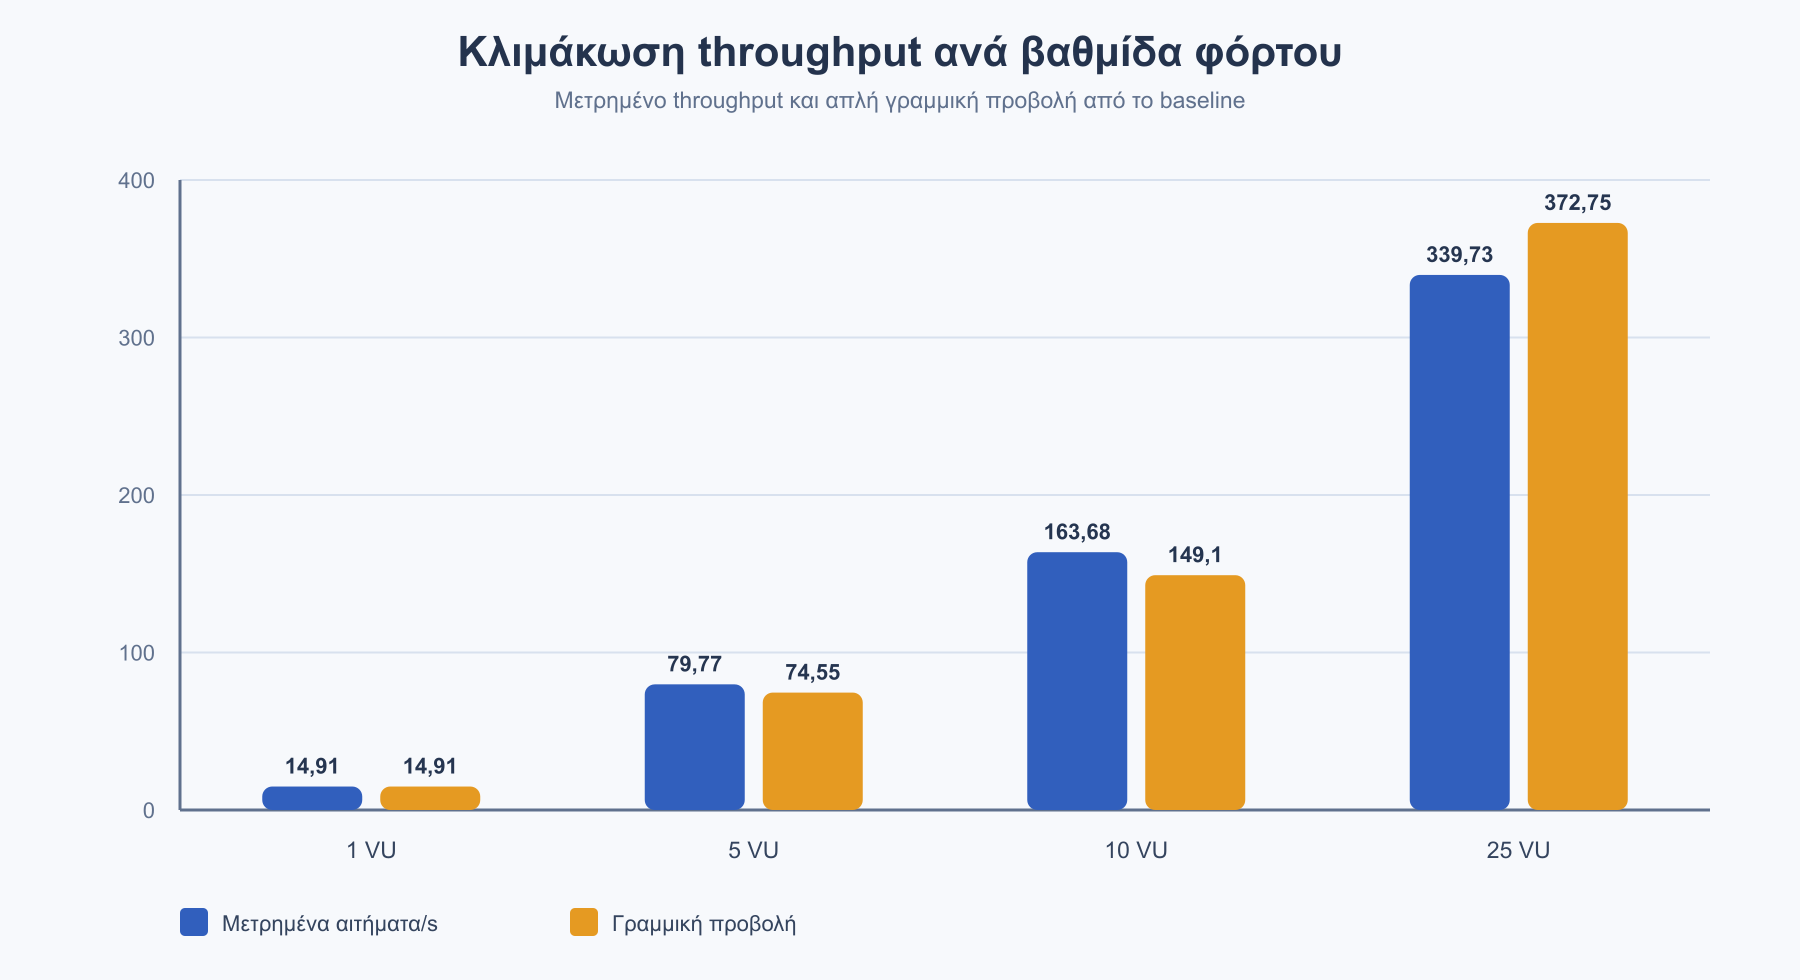
\includegraphics[width=\textwidth]{figures/evaluation/throughput-scaling.png}
\caption{Μετρημένο throughput ανά βαθμίδα φόρτου και σύγκριση με την απλή
γραμμική προβολή από το baseline.}
\label{fig:throughput-scaling}
\end{figure}

\begin{figure}[htbp]
\centering
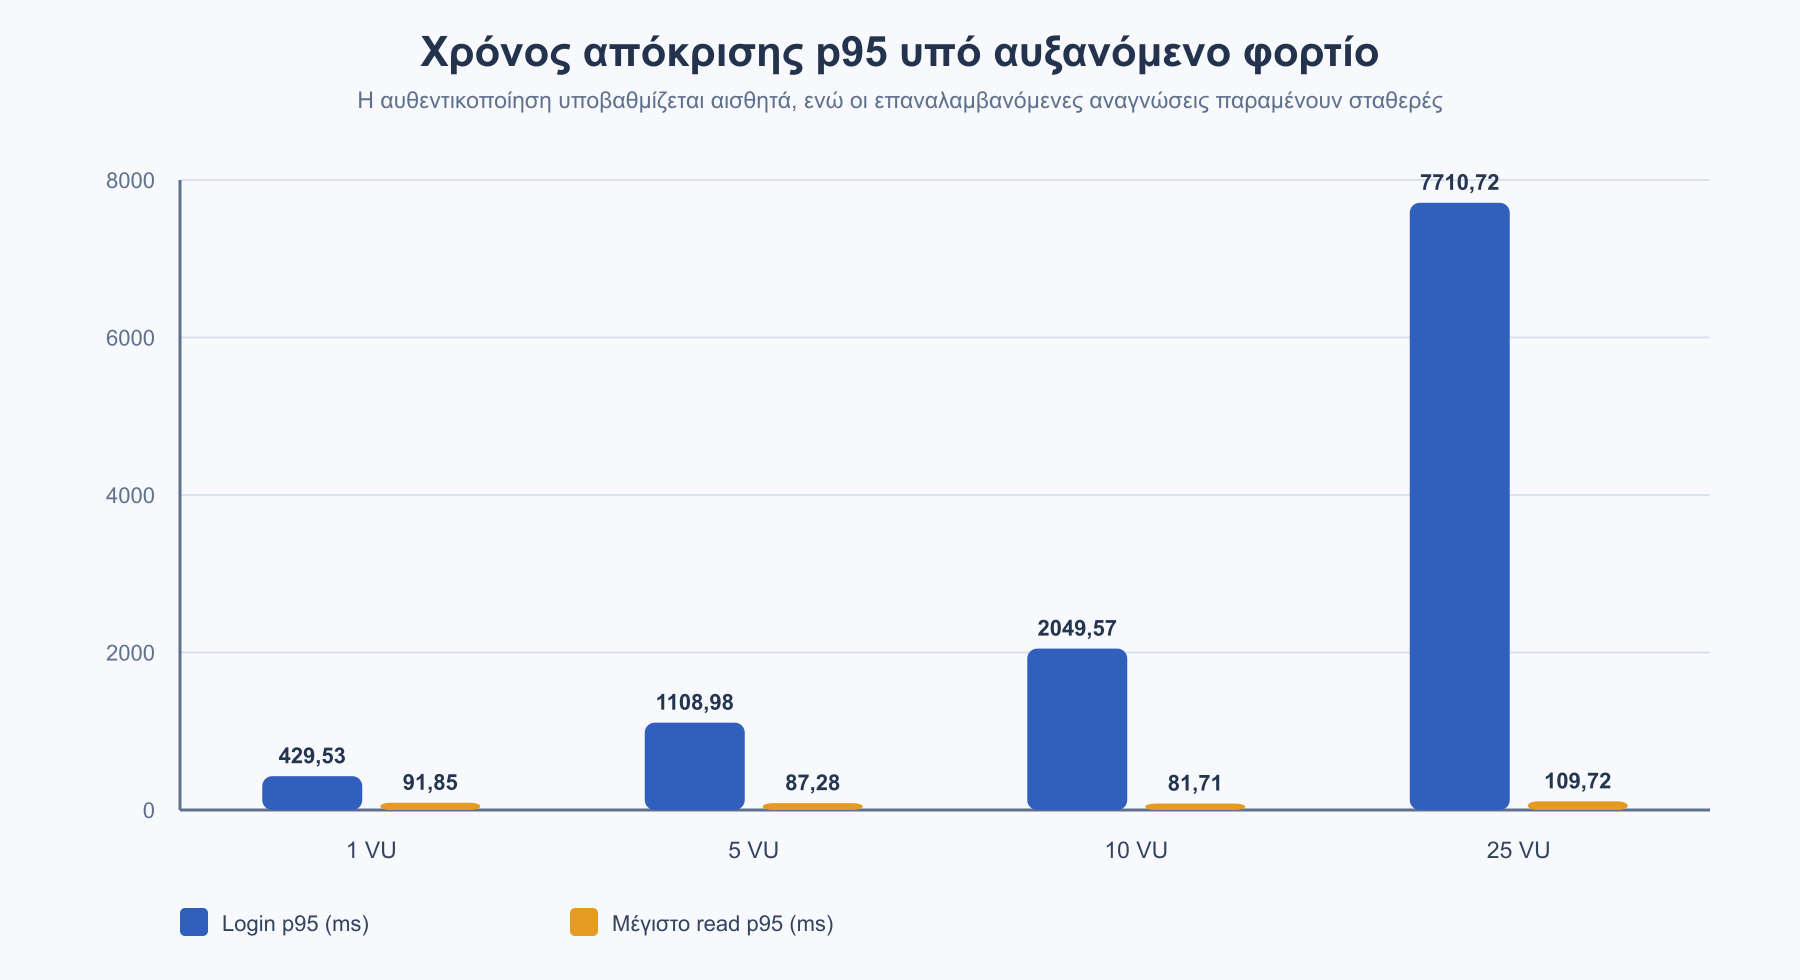
\includegraphics[width=\textwidth]{figures/evaluation/latency-p95-scaling.png}
\caption{Σύγκριση του p95 της αρχικής αυθεντικοποίησης με το υψηλότερο p95
των επαναλαμβανόμενων read endpoints ανά βαθμίδα φόρτου.}
\label{fig:latency-p95-scaling}
\end{figure}

Μετά από κάθε βαθμίδα, ο δημόσιος έλεγχος επέστρεψε HTTPS~200 και τα logs δεν
περιείχαν \texttt{ERROR}, exception ή \texttt{OutOfMemory}. Η στιγμιαία
χρήση μνήμης του Spring container αυξήθηκε από 399,3 σε 571,6~MiB, παραμένοντας
εντός του διαθέσιμου ορίου του instance. Στο πεντάλεπτο CloudWatch διάστημα
13:30--13:35~UTC, το οποίο περιλαμβάνει το τέλος της βαθμίδας των 10 χρηστών
και ολόκληρη τη βαθμίδα των 25, η μέση CPU ήταν 29,88\% και η μέγιστη
77,47\%. Καταγράφηκαν συνολικά 11.463.668 bytes εισόδου και 42.556.433 bytes
εξόδου, χωρίς αποτυχία status check. Επειδή οι σύντομες βαθμίδες τέμνουν τα
πεντάλεπτα aggregates και δύο από αυτές βρίσκονται στο ίδιο διάστημα, τα
metrics τεκμηριώνουν τη συνολική πίεση του high-load παραθύρου αλλά δεν
αποδίδονται αποκλειστικά σε μία βαθμίδα.

\begin{figure}[htbp]
\centering
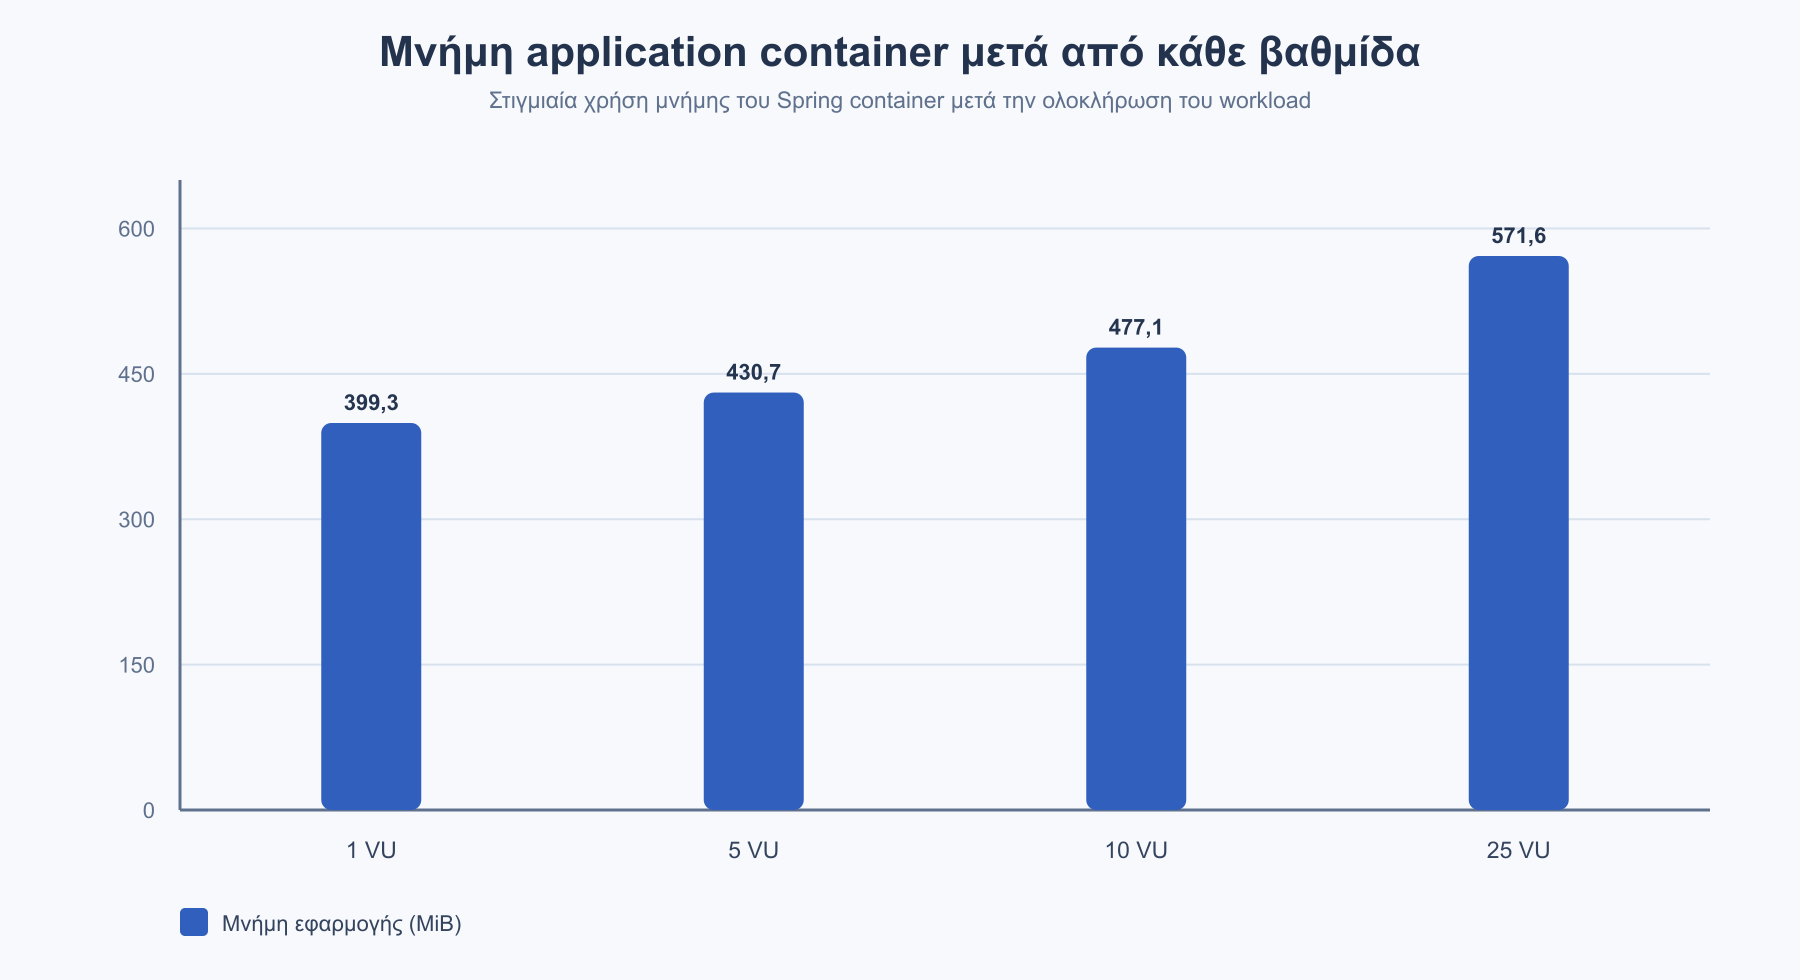
\includegraphics[width=\textwidth]{figures/evaluation/application-memory-scaling.png}
\caption{Στιγμιαία χρήση μνήμης του Spring container μετά από κάθε βαθμίδα
φόρτου. Οι τιμές αποτελούν μεταγενέστερα στιγμιότυπα και όχι μέγιστα της
ολόκληρης βαθμίδας.}
\label{fig:application-memory-scaling}
\end{figure}

Η βαθμίδα των 25 χρηστών χρησιμοποιήθηκε ως ελεγχόμενο stress endpoint και
εφαρμόστηκε το κριτήριο διακοπής: το login p95 είχε ήδη υπερβεί τα 7~s και η
μέγιστη CPU στο κοινό high-load παράθυρο έφθασε το 77,47\%. Η αύξηση πέρα
από αυτό το σημείο δεν ήταν αναγκαία για να αποδειχθεί η υποβάθμιση και θα
αύξανε άσκοπα τον κίνδυνο για τη μοναδική παραγωγική εγκατάσταση. Το όριο
αφορά το συγκεκριμένο πείραμα και δεν αποτελεί εγγυημένη παραγωγική
χωρητικότητα.

Στη συνέχεια εκτελέστηκε soak test πέντε εικονικών χρηστών για 300,29~s, από
13:36:51,714 έως 13:41:51,993~UTC. Ολοκληρώθηκαν 26.291 αιτήματα με
throughput 87,55 αιτήματα/s και μηδενικά σφάλματα. Τα p95 των τριών
αυθεντικοποιημένων read endpoints ήταν 64,16--67,65~ms και το μεγαλύτερο p95
όλων των reads ήταν 89,70~ms. Δεν παρατηρήθηκε χρονική αύξηση καθυστέρησης ή
αποτυχία διαθεσιμότητας. Σε ενδιάμεσο στιγμιότυπο το Spring container
χρησιμοποιούσε 570,9~MiB και 33,37\% CPU, ενώ η MySQL 499,8~MiB και 11,94\%
CPU.

Τα δύο πλήρη CloudWatch διαστήματα 13:35--13:40 και 13:40--13:45~UTC είχαν
μέση CPU 12,13\% και 12,57\%, μέγιστη 22,78\% και 23,43\% αντίστοιχα και
μηδενικό \texttt{StatusCheckFailed}. Συνολικά κατέγραψαν 10.854.409 bytes
εισόδου και 40.048.829 bytes εξόδου. Τα διαστήματα περιλαμβάνουν μικρό χρόνο
ηρεμίας πριν και μετά το πεντάλεπτο workload, αλλά δεν περιλαμβάνουν άλλη
δοκιμή φόρτου και παρέχουν καθαρότερη ένδειξη σταθερής χρήσης πόρων από τις
σύντομες βαθμίδες.

Η Εικόνα~\ref{fig:cloudwatch-cpu-windows} παρουσιάζει συγκεντρωτικά τη μέση
και τη μέγιστη CPU των πεντάλεπτων παραθύρων. Η κορύφωση στο διάστημα
13:30--13:35~UTC συμπίπτει με το τέλος της βαθμίδας των 10 χρηστών και τη
βαθμίδα των 25 χρηστών, ενώ τα δύο επόμενα παράθυρα αντιστοιχούν κυρίως στο
σταθερό soak workload. Η μέγιστη τιμή 77,47\% αποτελεί σύντομη αιχμή και όχι
παρατεταμένο κορεσμό του επεξεργαστή: η μέση τιμή του ίδιου παραθύρου ήταν
29,88\% και στα επόμενα δύο παράθυρα η μέγιστη χρήση υποχώρησε κάτω από
24\%. Ωστόσο, η αιχμή δείχνει ότι το διαθέσιμο περιθώριο CPU μειώνεται αισθητά
όταν αυξάνεται η ταυτόχρονη δραστηριότητα.

\begin{figure}[htbp]
\centering
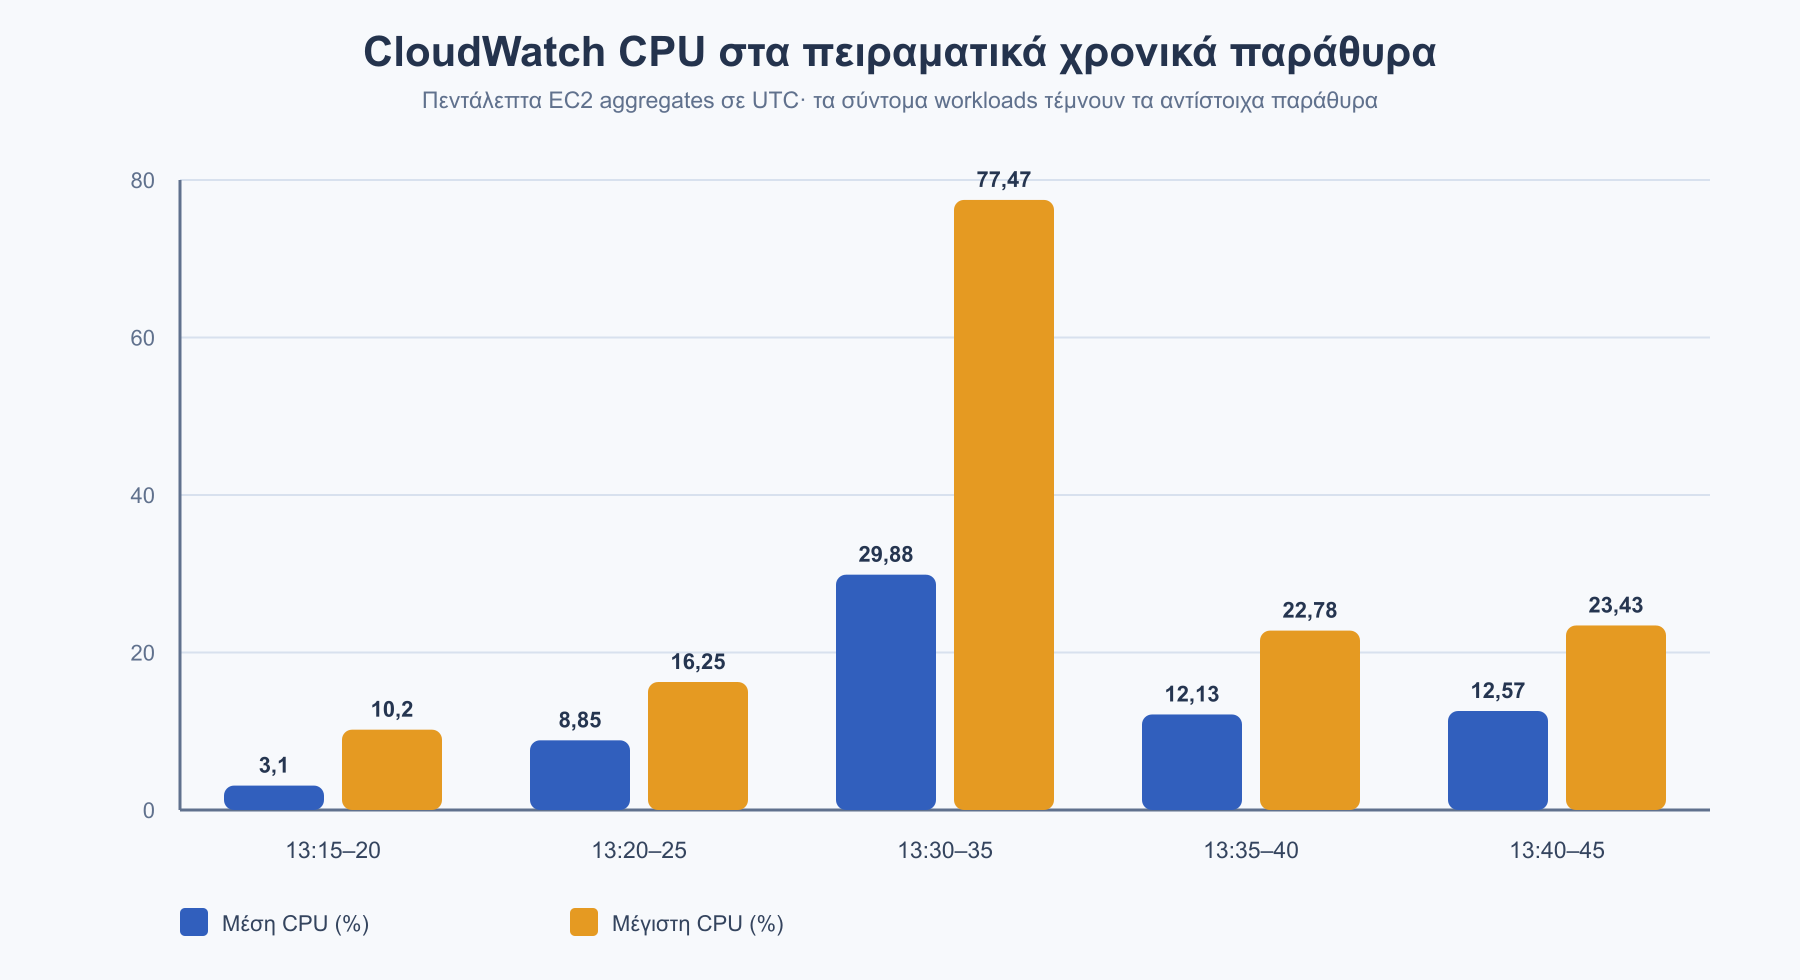
\includegraphics[width=\textwidth]{figures/evaluation/cloudwatch-cpu-windows.png}
\caption{Μέση και μέγιστη χρήση CPU του EC2 instance στα πεντάλεπτα
CloudWatch παράθυρα που συσχετίστηκαν με τις δοκιμές.}
\label{fig:cloudwatch-cpu-windows}
\end{figure}

\section{Αξιολόγηση αξιοπιστίας και επανεκκίνησης services}
Πραγματοποιήθηκε ελεγχόμενη επανεκκίνηση μόνο του
\texttt{petclinic-app}. Πριν από αυτήν καταγράφηκαν η φυσική διαδρομή ενός
δοκιμαστικού PDF, το ακριβές μέγεθος 1.191.697 bytes και το SHA-256 checksum
\texttt{6f2da0b1dc7721b3\ldots ba366c85564}. Μετά την επανεκκίνηση, η ίδια
διαδρομή παρέμενε διαθέσιμη, το μέγεθος και το checksum ήταν αμετάβλητα, το
container επέστρεψε σε κατάσταση \texttt{Up} και ο δημόσιος έλεγχος έδωσε
HTTPS~200. Τέλος, το πλήκτρο \enquote{Προβολή} ανέκτησε επιτυχώς το αρχείο.

\begin{figure}[htbp]
\centering
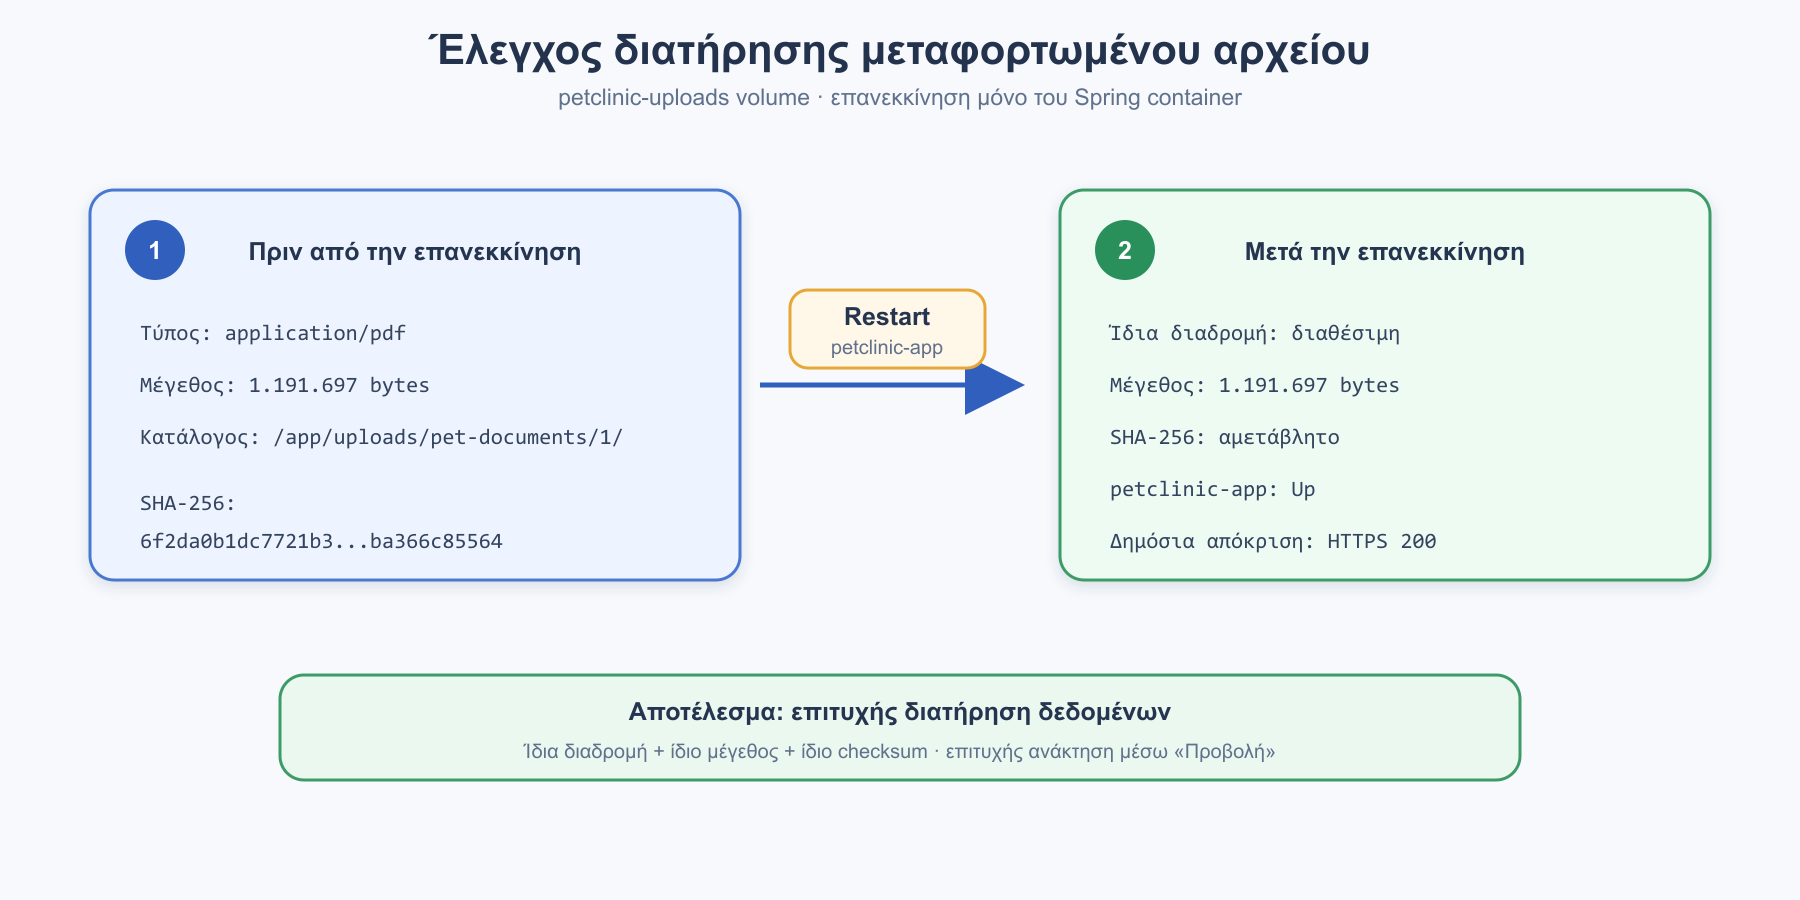
\includegraphics[width=\textwidth]{figures/infrastructure/upload-volume-persistence.png}
\caption{Επαλήθευση του persistent upload volume πριν και μετά την
επανεκκίνηση του Spring container. Η ταυτότητα του αρχείου επιβεβαιώνεται με
διαδρομή, μέγεθος και checksum, ενώ η ανάκτηση ελέγχεται από την εφαρμογή.}
\label{fig:upload-persistence-evaluation}
\end{figure}

Κατά την ίδια εκκίνηση το Liquibase ανέγνωσε τέσσερα changesets ως ήδη
εκτελεσμένα, δεν εκτέλεσε νέα μεταβολή και αποδέσμευσε επιτυχώς το changelog
lock. Το αποτέλεσμα αποτελεί ένδειξη επαναλήψιμης εκκίνησης χωρίς αυθαίρετη
τροποποίηση του schema. Δεν ισοδυναμεί όμως με πλήρη δοκιμή καταστροφής.

Στη συνέχεια πραγματοποιήθηκε ελεγχόμενο reboot ολόκληρου του EC2 instance.
Εξωτερικός watcher έλεγχε επαναληπτικά το δημόσιο HTTPS endpoint, ώστε η
μέτρηση να μην εξαρτάται από το ίδιο το instance. Η επανεκκίνηση ζητήθηκε στις
17:33:01~UTC. Η πρώτη αποτυχία καταγράφηκε στις 17:33:02,588~UTC και η πρώτη
απάντηση HTTP~200 στις 17:33:43,377~UTC, δηλαδή παρατηρήθηκε μη διαθεσιμότητα
40,79~s. Ακολούθησαν τρεις συνεχόμενες επιτυχείς απαντήσεις. Η ακολουθία των
παρατηρήσεων ήταν αποτυχία σύνδεσης, προσωρινή απάντηση HTTP~502 κατά την
εκκίνηση του upstream και τελικά HTTP~200.

Μετά το reboot τα τρία containers επανήλθαν αυτόματα μέσω πολιτικής
\texttt{unless-stopped}: το MySQL container ήταν \texttt{healthy} και τα
Spring και Nginx containers σε κατάσταση \texttt{Up}. Η εφαρμογή ολοκλήρωσε
την εκκίνησή της σε 18,352~s. Το αναπτυγμένο JAR διατήρησε το SHA-256
\texttt{317132aeac05f139\ldots de2153c82f3}, ενώ το δοκιμαστικό PDF διατήρησε
τόσο το μέγεθος 1.191.697 bytes όσο και το πλήρες checksum της προηγούμενης
μέτρησης. Τέλος, οι πληθικότητες των πινάκων ιδιοκτητών, κατοικιδίων, ραντεβού
και χρηστών παρέμειναν αντίστοιχα 2, 2, 2 και 3. Επομένως, στην ελεγχόμενη αυτή
δοκιμή επιβεβαιώθηκαν η αυτόματη επαναφορά των services και η διατήρηση βάσης
και uploads. Το αποτέλεσμα δεν αποτελεί απόδειξη υψηλής διαθεσιμότητας,
καθώς κατά το reboot υπήρξε αναμενόμενο διάστημα διακοπής.

\section{Έλεγχοι ασφάλειας}
Οι έλεγχοι που έχουν ήδη καταγραφεί επιβεβαιώνουν την ανακατεύθυνση HTTP σε
HTTPS, την απόρριψη λανθασμένων credentials και την απαγόρευση σύνδεσης σε
επιβεβαιωμένο αλλά μη εγκεκριμένο λογαριασμό. Οι διοικητικές λειτουργίες
εκτελέστηκαν από λογαριασμό με κατάλληλο ρόλο, ενώ τα tokens verification και
password reset αποθηκεύονται ως SHA-256 hashes και έχουν περιορισμένη διάρκεια
ζωής. Στις μεταφορτώσεις εφαρμόζεται όριο 10~MB και έλεγχος κανονικοποιημένης
διαδρομής ώστε το τελικό path να παραμένει εντός του upload root.

Στις 5 Σεπτεμβρίου 2026 εκτελέστηκε επαναλήψιμο σύνολο δέκα ελέγχων HTTP στην
παραγωγική εγκατάσταση. Οι δημόσιες σελίδες αρχικής και σύνδεσης επέστρεψαν
HTTP~200. Χωρίς authentication, τα endpoints dashboard, owners και
administration επέστρεψαν HTTP~401, ενώ η προσπάθεια σύνδεσης με λανθασμένο
κωδικό επέστρεψε επίσης HTTP~401. Μετά από έγκυρη σύνδεση συνθετικού χρήστη
με αποκλειστικό ρόλο \texttt{STAFF}, τα endpoints ταυτότητας και ανάγνωσης
owners επέστρεψαν HTTP~200, αλλά το διοικητικό endpoint επέστρεψε HTTP~403.
Όλοι οι αναμενόμενοι κωδικοί επιβεβαιώθηκαν, χωρίς να αποθηκευτούν
credentials, JWT ή response bodies στο τεκμήριο.

Εκτελέστηκε επίσης αρνητικός έλεγχος του ορίου μεταφόρτωσης. Συνθετικό αρχείο
10.485.761 bytes, δηλαδή ένα byte πάνω από το δηλωμένο όριο των 10~MiB,
υποβλήθηκε από τον ίδιο authenticated χρήστη και απορρίφθηκε με HTTP~413.
Μετά την απόρριψη επιβεβαιώθηκαν μηδενική νέα εγγραφή με τον δοκιμαστικό τίτλο
στον πίνακα \texttt{pet\_health\_records} και μηδενικό αντίστοιχο αρχείο στο
persistent upload volume. Το προσωρινό τοπικό payload διαγράφηκε.

Η επισκόπηση του κώδικα έδειξε ότι η τρέχουσα έκδοση περιορίζει το μέγεθος και
την τελική διαδρομή, αλλά δεν εφαρμόζει allowlist τύπων MIME ή επεκτάσεων.
Επομένως δεν παρουσιάζεται ανύπαρκτος έλεγχος \enquote{μη επιτρεπτού τύπου}
ως επιτυχής· η προσθήκη allowlist καταγράφεται ως πρόταση σκλήρυνσης. Για την
ολοκλήρωση της σκλήρυνσης προτείνεται ο συνδυασμός allowlist, ελέγχου
πραγματικού περιεχομένου και αποθήκευσης εκτός web root.

Ο έλεγχος εξαρτήσεων εκτελέστηκε σε δύο επίπεδα. Το \texttt{npm audit}, το
οποίο αντιπαραβάλλει το dependency tree του lockfile με τα advisories του
registry \cite{npm2026audit}, ανέφερε για τις 64 production frontend
dependencies δύο ευάλωτα packages υψηλής σοβαρότητας:
\texttt{react-router-dom} ως άμεση εξάρτηση και \texttt{react-router} ως
μεταβατική, με διαθέσιμη διόρθωση. Όταν συμπεριλήφθηκαν και οι build-time
εξαρτήσεις, αναφέρθηκαν 15 packages συνολικά: 12 υψηλής, 2 μέτριας και 1
χαμηλής σοβαρότητας. Ο διαχωρισμός είναι σημαντικός, επειδή εργαλεία όπως
Vite και ESLint χρησιμοποιούνται κατά το build και δεν εκτελούνται ως Node
services στην παραγωγή.

Παράλληλα, το ακριβές deployed Docker image
\texttt{sha256:1b1a0980\ldots ba47835e} σαρώθηκε με Trivy~0.73.0, το οποίο
αναλύει τόσο OS packages όσο και βιβλιοθήκες εφαρμογής σε container images
\cite{aquasecurity2026trivyimage}. Καταγράφηκαν 250 advisory matches: 9
critical, 34 high, 160 medium και 47 low. Η κατανομή ήταν 161 low/medium
ευρήματα στο Ubuntu base layer, 81 στη Java layer και 8 high στο βοηθητικό
binary \texttt{pebble}. Και τα 9 critical ευρήματα βρίσκονταν στη Java layer,
κυρίως στις παλαιότερες εκδόσεις embedded Tomcat και Spring Security που
κληρονομούνται από το Spring Boot~3.2.8. Η ενδεδειγμένη αποκατάσταση είναι
αναβάθμιση του Spring Boot dependency train και του React Router, επιλογή
ενημερωμένου και μικρότερου runtime base image, rebuild και επανάληψη των
regression/security tests.

Τα παραπάνω αποτελέσματα αποτελούν αντιστοιχίσεις αυτοματοποιημένων βάσεων
advisories και όχι απόδειξη ότι κάθε CVE είναι εκμεταλλεύσιμο στη συγκεκριμένη
διαμόρφωση. Απαιτείται triage ως προς τη χρησιμοποιούμενη λειτουργία, τις
προϋποθέσεις κάθε CVE και την πραγματική προσβασιμότητα. Ωστόσο, η ύπαρξη
διαθέσιμων fixed versions, ιδιαίτερα για critical runtime components,
καθιστά την αναβάθμιση απαραίτητο βήμα πριν από χρήση πέρα από το πλαίσιο της
διπλωματικής επίδειξης.

Η τελική μέτρηση TLS έδειξε ότι το Nginx επιτρέπει αποκλειστικά TLS~1.2 και
TLS~1.3· και οι δύο εκδόσεις διαπραγματεύτηκαν επιτυχώς με AEAD cipher suites.
Το πιστοποιητικό Let's Encrypt είχε subject
\texttt{CN=thesis-tasiopoulos.com}, κάλυπτε επιπλέον το
\texttt{www.thesis-tasiopoulos.com} και ήταν έγκυρο από 31 Αυγούστου έως 29
Νοεμβρίου 2026. Το HTTP endpoint επέστρεψε 301, το HTTPS endpoint 200 και
παρατηρήθηκε ο header \path{Strict-Transport-Security}, με διάρκεια ενός
έτους και την οδηγία \path{includeSubDomains}. Καταγράφηκαν επίσης ο
\path{X-Content-Type-Options} με τιμή \path{nosniff} και Content
Security Policy που περιορίζει το \path{frame-ancestors} στα δύο ονόματα
του domain.

\section{Οικονομική αξιολόγηση}
Η CloudFront distribution εντάχθηκε στο Free flat-rate plan, για το οποίο η
κονσόλα εμφάνισε \texttt{\$0/month} και εκτιμώμενη χρέωση ημέρας
\texttt{\$0}. Το plan περιλαμβάνει συγκεκριμένα μηνιαία όρια χρήσης και δεν
χρεώνει υπερβάσεις, σύμφωνα με την τεκμηρίωση της AWS
\cite{aws2026cloudfrontplans}. Η παρατήρηση αφορά αποκλειστικά τη χρέωση του
CloudFront plan και δεν αναιρεί πιθανές χρεώσεις της προϋπάρχουσας υποδομής.

Στις 7 Σεπτεμβρίου 2026, μετά την καθυστερημένη ενημέρωση των στοιχείων
χρέωσης, το Cost Explorer ρυθμίστηκε με net unblended cost, εξαίρεση refunds
και credits και ομαδοποίηση ανά υπηρεσία. Για τον τρέχοντα κύκλο του
Σεπτεμβρίου εμφάνισε εκτιμώμενο κόστος κατανάλωσης \texttt{\$5.38}. Η
πρόβλεψη της AWS για το τέλος του μήνα ήταν \texttt{\$9.59}, εφόσον
διατηρούνταν αντίστοιχο μοτίβο χρήσης, ενώ το συνολικό κόστος του Αυγούστου
ήταν \texttt{\$1.04}. Οι τιμές του τρέχοντος billing period παραμένουν
προσωρινές: το Cost Explorer ανανεώνει τα δεδομένα τουλάχιστον μία φορά ανά
24 ώρες και μπορεί να διαφέρει προσωρινά από τη σελίδα Bills λόγω χρόνου
ενημέρωσης και στρογγυλοποίησης
\cite{aws2026costexplorer,aws2026billingdifferences}.

Ο Πίνακας~\ref{tab:aws-observed-costs} παρουσιάζει την κατανομή του
καταγεγραμμένου κόστους. Το EC2 compute ήταν ο κυρίαρχος παράγοντας με
\texttt{\$3.51}, περίπου 65,2\% του συνόλου. Ακολουθούσαν το VPC με
\texttt{\$0.74}, το EC2--Other με \texttt{\$0.62} και το Route~53 με
\texttt{\$0.50}. Οι επιμέρους τιμές δεν αθροίζουν ακριβώς στο εμφανιζόμενο
σύνολο λόγω στρογγυλοποίησης σε δύο δεκαδικά ψηφία.

\begin{table}[htbp]
\centering
\caption{Παρατηρημένο κόστος AWS για τον Σεπτέμβριο έως 7/9/2026.}
\label{tab:aws-observed-costs}
\small
\begin{tabularx}{0.92\textwidth}{Xrr}
\toprule
Υπηρεσία & Κόστος (USD) & Μερίδιο συνόλου \\
\midrule
EC2 compute & \texttt{\$3.51} & 65,2\% \\
VPC & \texttt{\$0.74} & 13,8\% \\
EC2--Other & \texttt{\$0.62} & 11,5\% \\
Route~53 & \texttt{\$0.50} & 9,3\% \\
SES, S3, CloudWatch, CloudFront, KMS, Glue και CloudShell & \texttt{\$0.00} ανά υπηρεσία & $<$0,1\% \\
\midrule
Σύνολο Cost Explorer & \texttt{\$5.38} & 100\% \\
\bottomrule
\end{tabularx}
\end{table}

Η σελίδα Bills εμφάνιζε ταυτόχρονα εκτιμώμενο πληρωτέο ποσό
\texttt{\$0.00}, επειδή ενεργές προωθητικές πιστώσεις κάλυπταν την
κατανάλωση. Επομένως διακρίνονται δύο διαφορετικά μεγέθη: το κόστος των
πόρων που κατανάλωσε η εγκατάσταση και το ποσό που τελικά επιβαρύνει τον
χρήστη μετά την εφαρμογή πιστώσεων. Οι πιστώσεις αποτελούν προσωρινό όφελος
του συγκεκριμένου λογαριασμού και δεν χρησιμοποιούνται ως βάση για την
εκτίμηση του κανονικού λειτουργικού κόστους. Με τα δεδομένα της παρατήρησης,
η πειραματική λειτουργία αντιστοιχεί σε τάξη μεγέθους περίπου
\texttt{\$9--10} ανά μήνα, όχι σε μηδενικό οικονομικό κόστος.

Ξεχωριστά από το CloudFront Free plan, το πρόγραμμα AWS Free Tier για νέους
πελάτες προβλέπει αρχική πίστωση και δυνατότητα απόκτησης πρόσθετων πιστώσεων
με την ολοκλήρωση εκπαιδευτικών δραστηριοτήτων που εμφανίζονται στο
\enquote{Explore AWS}, όπως η εκκίνηση EC2 instance ή η δημιουργία budget.
Οι πιστώσεις αυτές είναι προσωρινές και καλύπτουν επιλέξιμες χρεώσεις· δεν
μετατρέπουν την πραγματική κατανάλωση πόρων σε μηδενικό κόστος
\cite{aws2026freetieractivities}.

Ο Πίνακας~\ref{tab:aws-cost-drivers} συνοψίζει τα στοιχεία που θα
δημιουργούσαν χρέωση χωρίς πιστώσεις. Οι τιμές είναι τιμές καταλόγου χωρίς
φόρους και όχι δεσμευτική προσφορά· η τελική χρέωση εξαρτάται από τις ώρες
λειτουργίας, την κίνηση και την ισχύ των εκάστοτε Free Tier παροχών.

\begin{table}[htbp]
\centering
\caption{Κύριοι παράγοντες κόστους της πειραματικής εγκατάστασης.}
\label{tab:aws-cost-drivers}
\small
\begin{tabularx}{\textwidth}{p{0.19\textwidth}p{0.31\textwidth}X}
\toprule
Υπηρεσία & Μονάδα χρέωσης & Εφαρμογή στην εγκατάσταση \\
\midrule
EC2 & Χρόνος λειτουργίας του instance, ανά δευτερόλεπτο με ελάχιστο 60~s & Το \texttt{t3.small} είναι ο βασικός επαναλαμβανόμενος υπολογιστικός πόρος· η χρέωση compute σταματά όταν το instance σταματήσει \cite{aws2026ec2pricing}. \\
EBS & Provisioned GB ανά μήνα & Το volume \texttt{gp3} των 30~GiB συνεχίζει να χρεώνεται όσο παραμένει δεσμευμένο, ακόμη και με σταματημένο EC2· τα βασικά 3.000 IOPS και 125~MB/s περιλαμβάνονται \cite{aws2026ebspricing}. \\
Public IPv4 & \texttt{\$0.005} ανά διεύθυνση και ώρα & Μία διεύθυνση επί 30 ημέρες αντιστοιχεί περίπου σε \texttt{\$3.60}, είτε είναι σε χρήση είτε παραμένει δεσμευμένη \cite{aws2026vpcpricing}. \\
Route~53 & \texttt{\$0.50} ανά hosted zone τον μήνα και \texttt{\$0.40}/εκατ. standard queries & Η κατοχύρωση του \texttt{.com} χρεώνεται χωριστά σε ετήσια βάση· το χαμηλό πειραματικό DNS traffic είναι πρακτικά αμελητέο \cite{aws2026route53pricing}. \\
SES & \texttt{\$0.10}/1.000 outbound emails και \texttt{\$0.12}/GB εξερχόμενων δεδομένων & Οι λίγες staff verification και password-reset αποστολές έχουν κόστος πολύ μικρότερο του ενός cent· δεν χρησιμοποιήθηκαν dedicated IPs \cite{aws2026sespricing}. \\
CloudWatch & Βασικά service metrics χωρίς πρόσθετη χρέωση· detailed/custom metrics και logs με χρέωση & Χρησιμοποιήθηκαν μόνο τα προεπιλεγμένα πεντάλεπτα EC2 metrics και status checks, χωρίς Agent ή log ingestion \cite{aws2026cloudwatchbasic}. \\
S3 & Αποθήκευση, requests και μεταφορά δεδομένων & Το προσωρινό deployment object περίπου 70,5~MB δημιουργεί αμελητέα αποθήκευση και ελάχιστα requests· η εισερχόμενη μεταφορά και η μεταφορά προς υπηρεσία στην ίδια περιοχή δεν χρεώνονται \cite{aws2026s3pricing}. \\
CloudFront & Free flat-rate plan: \texttt{\$0/month} & Περιλαμβάνει έως 1 εκατ. requests και 100~GB transfer τον μήνα χωρίς overage charge, όρια κατά πολύ μεγαλύτερα από το PoC \cite{aws2026cloudfrontplans}. \\
\bottomrule
\end{tabularx}
\end{table}

Η ανάλυση διαχωρίζει EC2, EBS, Route~53, data transfer, SES και CloudWatch,
ώστε να μην αποδίδεται ολόκληρο το κόστος σε μία μόνο υπηρεσία. Για τη
συσχέτιση των πειραμάτων χρησιμοποιήθηκαν μόνο τα βασικά EC2 metrics και τα
status checks. Δεν εγκαταστάθηκε CloudWatch Agent και δεν δημιουργήθηκαν
custom metrics ή πρόσθετη συλλογή logs, συνεπώς η αξιολόγηση δεν εισήγαγε
τέτοια πρόσθετη χρέωση. Ως προληπτικό μέτρο προετοιμάστηκε AWS Budget
μηδενικής δαπάνης, με προτεινόμενη ειδοποίηση όταν η καταγεγραμμένη δαπάνη
υπερβεί τα \texttt{\$0.01}. Η ενεργοποίηση της ειδοποίησης δεν αποτελεί
μέρος της μέτρησης και μπορεί να γίνει πριν παραμείνει η υποδομή ενεργή για
μεγαλύτερο διάστημα. Δεν παρουσιάζονται account identifiers, διευθύνσεις
ειδοποίησης ή στοιχεία πληρωμής.

\section{Συζήτηση αποτελεσμάτων και περιορισμών}
Τα έως τώρα αποτελέσματα δείχνουν ότι η μονοκομβική containerized εγκατάσταση
είναι λειτουργική, χρησιμοποιεί έγκυρο HTTPS, εκτελεί επαναλήψιμες migrations
και διατηρεί μεταφορτωμένα δεδομένα όταν αντικαθίσταται ή επανεκκινείται το
application container. Η επιτυχής ανάκτηση του PDF από τη διεπαφή είναι
ισχυρότερη ένδειξη από την απλή ύπαρξη του αρχείου στο filesystem, επειδή
ελέγχει ταυτόχρονα metadata, backend endpoint και browser flow.

Τα ευρήματα δεν αποδεικνύουν υψηλή διαθεσιμότητα. Υπάρχει ένα EC2 instance,
μία MySQL και ένα application container, χωρίς load balancer ή δεύτερη ζώνη
διαθεσιμότητας. Το reboot επιβεβαίωσε την αυτόματη επαναφορά, αλλά κατέγραψε
διακοπή 40,79~s και δεν υποκαθιστά δοκιμή restore από backup ή αστοχία
ολόκληρης ζώνης διαθεσιμότητας. Οι περιορισμοί αυτοί παραμένουν ρητοί κατά
την ερμηνεία των load, stress, soak και cost results.

\section{Κατάλογος ολοκληρωμένων ελέγχων και τεκμηρίων}
Ο Πίνακας~\ref{tab:evaluation-status} λειτουργεί ως συνοπτικός χάρτης των
ελέγχων που παρουσιάστηκαν αναλυτικά στις προηγούμενες ενότητες. Δεν
αποτελεί εσωτερικό πίνακα παρακολούθησης εργασιών: καταγράφει το αντικείμενο
κάθε δοκιμής, το παρατηρηθέν αποτέλεσμα και το τεκμήριο στο οποίο βασίζεται,
ώστε ο αναγνώστης να μπορεί να εντοπίσει γρήγορα το εύρος της αξιολόγησης.

\begin{table}[htbp]
\centering
\caption{Κατάλογος ολοκληρωμένων ελέγχων και κύριων τεκμηρίων.}
\label{tab:evaluation-status}
\small
\begin{tabularx}{\textwidth}{p{0.34\textwidth}p{0.20\textwidth}X}
\toprule
Αντικείμενο ελέγχου & Αποτέλεσμα & Κύριο τεκμήριο \\
\midrule
Λειτουργικές ροές και SES & Επιτυχία & Εγγραφή, verification, approval και reset \\
DNS, HTTP και HTTPS & Επιτυχία & DNS resolution, 301 redirect και HTTPS 200 \\
Liquibase restart & Επιτυχία & 4 previously run, 0 νέα changesets \\
Upload και προβολή PDF & Επιτυχία & Metadata και επιτυχής ανάκτηση στον browser \\
Persistence μετά από app restart & Επιτυχία & Ίδιο path, μέγεθος και SHA-256 \\
CloudFront proof of concept & Επιτυχία & Free plan, HTTPS origin, HTTP redirect, αρχική σελίδα και \texttt{/login} \\
Response-time baseline & Επιτυχία & 895 αιτήματα, 14,91 requests/s και 0 σφάλματα \\
Load stages 1/5/10/25 VU & Επιτυχία με εμφανές όριο & 0 σφάλματα έως 339,73 requests/s και υποβάθμιση login \\
Stress/soak & Επιτυχία & Stop point στα 25 VU και 5 VU για 300~s χωρίς σφάλματα \\
CloudWatch correlation & Επιτυχία & CPU, network και status checks για baseline, load και soak \\
EC2 reboot & Επιτυχία με μετρημένη διακοπή & Αυτόματη επαναφορά, persistence και HTTPS σε 40,79~s \\
Security matrix & Επιτυχία εντός πεδίου & API/RBAC, όριο upload, dependency scan και TLS \\
Πραγματικό κόστος & Καταγράφηκε & Cost Explorer, Bills, credits και τιμές καταλόγου ανά υπηρεσία \\
\bottomrule
\end{tabularx}
\end{table}



\chapter{Συμπεράσματα και Μελλοντικές Επεκτάσεις}
\section{Σύνοψη της εργασίας}
Η εργασία ξεκίνησε από ένα πρακτικό ερώτημα: πώς μπορεί μία πραγματική
εφαρμογή διαχείρισης κτηνιατρικής κλινικής να μεταφερθεί στο υπολογιστικό
νέφος χωρίς η υποδομή να γίνει δυσανάλογα ακριβή ή δύσκολη στη συντήρηση;
Το Happy Tails δεν αντιμετωπίστηκε ως απομονωμένο τεχνολογικό δείγμα, αλλά
ως σύστημα που χειρίζεται λογαριασμούς προσωπικού, κηδεμόνες, ζώα, ραντεβού,
ιατρικές εγγραφές και έγγραφα. Η αξιολόγηση έπρεπε επομένως να καλύπτει
λειτουργικότητα, ασφάλεια, διατήρηση δεδομένων, επιδόσεις, επαναφορά και κόστος.

Η τελική εγκατάσταση βασίστηκε σε μία EC2 instance στην περιοχή Frankfurt,
με Amazon Linux~2023 και τρία Docker containers: Nginx, Spring Boot και
MySQL. Το EBS παρείχε μόνιμη αποθήκευση, η Elastic IP και το Route~53
σταθερό δημόσιο σημείο πρόσβασης και το Nginx ασφαλή έκθεση μέσω HTTPS. Η
εφαρμογή συμπληρώθηκε με Amazon SES για τις ροές λογαριασμών προσωπικού και
με Google Calendar OAuth για τον συγχρονισμό ραντεβού. Οι δύο μηχανισμοί
παραμένουν διακριτοί: το SES μεταφέρει μηνύματα της εφαρμογής, ενώ το Google
Calendar δημιουργεί γεγονότα και προσκλήσεις.

Η εγκατάσταση δεν αξιολογήθηκε μόνο με στιγμιότυπα οθόνης. Ελέγχθηκαν οι
βασικές ροές, η επαναληψιμότητα των Liquibase migrations, η διατήρηση ενός
PDF μετά από επανεκκίνηση, οι ρόλοι, οι αποκρίσεις HTTP και η συμπεριφορά υπό
κλιμακούμενο φορτίο. Τα αποτελέσματα συσχετίστηκαν με CloudWatch metrics και
πραγματοποιήθηκε ελεγχόμενο reboot ολόκληρου του instance. Εξετάστηκαν ακόμη
οι εξαρτήσεις, το TLS και οι πραγματικοί παράγοντες κόστους. Το αποτέλεσμα
είναι συνεπώς τόσο μία λειτουργική εγκατάσταση όσο και μία αναπαραγώγιμη
διαδικασία αξιολόγησής της.

\section{Κύρια συμπεράσματα}
Το πρώτο συμπέρασμα είναι ότι μία μικρή containerized εγκατάσταση μπορεί να
καλύψει αξιόπιστα έναν περιορισμένο και σαφώς ορισμένο φόρτο. Δεν
παρατηρήθηκαν σφάλματα στα load stages, ακόμη και στη βαθμίδα των 25 VU. Η
υποβάθμιση της αρχικής αυθεντικοποίησης και η στιγμιαία αιχμή CPU έδειξαν
όμως ότι η χωρητικότητα δεν είναι απεριόριστη. Η καθυστέρηση μπορεί να γίνει
μη αποδεκτή πριν η εφαρμογή αρχίσει να επιστρέφει αποτυχημένες αποκρίσεις.

Το δεύτερο συμπέρασμα αφορά τη διαφορά ανάμεσα στην αυτόματη επανεκκίνηση
και στην υψηλή διαθεσιμότητα. Η πολιτική Docker
\texttt{restart: unless-stopped} επανέφερε τα services, το Liquibase δεν
επανεκτέλεσε ήδη εφαρμοσμένες αλλαγές και τα δεδομένα διατηρήθηκαν. Ωστόσο,
το reboot προκάλεσε διακοπή 40,79~s. Άρα υπάρχει μηχανισμός ανάκαμψης, αλλά
όχι πλεονασμός: όσο υπάρχει ένας μόνο κόμβος, η βλάβη ή συντήρησή του
επηρεάζει ολόκληρη την υπηρεσία.

Η επιλογή Spring Boot και React παρέμεινε κατάλληλη μετά τη μετάβαση στο
νέφος. Το Spring Boot παρέχει σαφή διαχωρισμό επιπέδων, ενσωμάτωση με Spring
Security και εξωτερική παραμετροποίηση~\cite{spring2026boot}. Η React
επιτρέπει επαναχρησιμοποιήσιμα στοιχεία διεπαφής και single-page εφαρμογή
\cite{react2026docs}. Ο συνδυασμός δεν εξαρτάται από μία συγκεκριμένη AWS
υπηρεσία: μπορεί να εκτελεστεί σε μία EC2 instance, σε πολλούς κόμβους ή ως
managed container workload. Αυτή η φορητότητα είναι σημαντικότερη από την
απλή χρήση πολλών cloud services.

Οι σαρώσεις έδειξαν επίσης ότι η συντήρηση των εξαρτήσεων είναι συνεχής
λειτουργική υποχρέωση. Εντοπίστηκαν διορθώσιμες ευπάθειες στο frontend tree
και στο deployed image. Η επόμενη έκδοση πρέπει επομένως να αναβαθμίσει το
Spring Boot dependency train, το React Router και το runtime base image και
να επαναλάβει τα regression, security και load tests.

Τέλος, το πραγματικό κόστος δεν ταυτίζεται με το ποσό που εμφανίζεται ως
πληρωτέο. Οι πιστώσεις οδήγησαν σε μηδενική πληρωμή, παρότι υπήρχε μετρήσιμη
χρήση. Η αξιολόγηση πρέπει να λαμβάνει υπόψη τις μονάδες χρέωσης EC2, EBS,
IPv4, Route~53, SES και CloudWatch, αλλά και τον χρόνο χειροκίνητης
διαχείρισης. Μία φθηνότερη υπηρεσία δεν είναι πάντοτε φθηνότερη συνολικά αν
μεταφέρει μεγάλο λειτουργικό βάρος στον διαχειριστή.

\section{Απάντηση στα ερευνητικά ερωτήματα}
\subsection*{ΕΕ1: Καταλληλότητα της οικονομικά περιορισμένης εγκατάστασης}
Η εγκατάσταση υποστήριξε τις βασικές λειτουργίες της κλινικής:
αυθεντικοποίηση και ρόλους, κηδεμόνες και ζώα, ραντεβού, ιατρικές εγγραφές,
έγγραφα, email λογαριασμού και ημερολόγιο. Η ανάπτυξη είναι επαναλήψιμη μέσω
Docker Compose και Liquibase και η δημόσια πρόσβαση προστατεύεται με HTTPS
και περιορισμένους κανόνες δικτύου. Η απάντηση στο ΕΕ1 είναι θετική για το
συγκεκριμένο εύρος και μέγεθος χρήσης, όχι όμως για απεριόριστο φορτίο ή
απαίτηση αδιάλειπτης λειτουργίας.

\subsection*{ΕΕ2: Επιδόσεις, πόροι και επανεκκίνηση}
Η εγκατάσταση διατήρησε μηδενικά σφάλματα στα load stages και ολοκλήρωσε το
soak test χωρίς απώλεια διαθεσιμότητας. Τα read endpoints παρέμειναν σχετικά
σταθερά, ενώ η αρχική αυθεντικοποίηση αποτέλεσε το πρώτο εμφανές σημείο
υποβάθμισης. Η CPU έφθασε στιγμιαία το 77,47\%, χωρίς παρατεταμένο κορεσμό.
Μετά το reboot η δημόσια υπηρεσία επανήλθε σε 40,79~s και τα δεδομένα
παρέμειναν αναλλοίωτα. Η συμπεριφορά ήταν σταθερή για το πειραματικό φορτίο,
αλλά ο χρόνος επαναφοράς επιβεβαιώνει τον περιορισμό του μοναδικού κόμβου.

\subsection*{ΕΕ3: Περιορισμοί και managed services}
Τα κύρια single points of failure είναι η μοναδική EC2 instance, η MySQL
στο ίδιο host και το τοπικά προσαρτημένο upload volume. Επιπλέον, τα μυστικά
βρίσκονται σε προστατευμένο αρχείο περιβάλλοντος, η παρακολούθηση βασίζεται
κυρίως σε προεπιλεγμένες μετρικές και το deployment περιλαμβάνει χειροκίνητα
βήματα. Οι περιορισμοί μπορούν να μειωθούν με Application Load Balancer
(ALB) και Auto Scaling σε περισσότερες Availability Zones, RDS Multi-AZ, S3 για τα
uploads, Secrets Manager, CloudWatch alarms, AWS Backup και WAF. Η επιλογή
πρέπει να γίνεται ανάλογα με την κρισιμότητα και όχι μόνο επειδή μία υπηρεσία
είναι διαθέσιμη.

\subsection*{ΕΕ4: Κόστος και συμβιβασμοί}
Η υλοποιημένη λύση έχει μικρό άμεσο κόστος και είναι εύκολη στην κατανόηση,
αλλά συγκεντρώνει compute, database και αρχεία στον ίδιο κόμβο. Μία λύση
υψηλότερης διαθεσιμότητας αυξάνει το σταθερό κόστος μέσω load balancer,
πολλαπλών targets, managed database, backups και αυξημένης παρακολούθησης.
Σε αντάλλαγμα μειώνει τον κίνδυνο διακοπής και επιτρέπει ανεξάρτητη κλιμάκωση
εφαρμογής και δεδομένων. Για μία μικρή κλινική η παρούσα λύση είναι λογικό
πρώτο στάδιο. Για πολλές κλινικές ή 24ωρη επιχειρησιακή εξάρτηση, το πρόσθετο
κόστος του πλεονασμού γίνεται δικαιολογημένο.

\section{Περιορισμοί}
Η μελέτη αφορά πραγματική αλλά μικρής κλίμακας εγκατάσταση. Το dataset, οι
λογαριασμοί και η διάρκεια των δοκιμών είναι περιορισμένα. Τα VU εκτελούν
συγκεκριμένες ακολουθίες HTTP και δεν προσομοιώνουν πλήρως την ανθρώπινη
συμπεριφορά, αργές συνδέσεις ή τη μακροχρόνια αύξηση δεδομένων. Ένα soak test
πέντε λεπτών μπορεί να εντοπίσει άμεσα προβλήματα, όχι όμως διαρροές πόρων που
εμφανίζονται μετά από ώρες ή ημέρες.

Το reboot αξιολόγησε την επαναφορά του υπάρχοντος instance, όχι την απώλεια
Availability Zone. Δεν πραγματοποιήθηκε restore σε νέο περιβάλλον ούτε
μετρήθηκαν Recovery Time Objective (RTO) και Recovery Point Objective (RPO)
μέσα από πλήρη άσκηση καταστροφής. Η επιτυχής persistence δεν αποτελεί από
μόνη της απόδειξη επαρκούς στρατηγικής backup.

Οι έλεγχοι ασφάλειας δεν αντικαθιστούν penetration test, ανεξάρτητη
ανασκόπηση κώδικα ή έλεγχο συμμόρφωσης. Για έγγραφα και στοιχεία επικοινωνίας
απαιτούνται πολιτικές διατήρησης, audit και ελαχιστοποίησης δεδομένων που
υπερβαίνουν το πεδίο της εργασίας. Τέλος, το κόστος επηρεάζεται από credits,
Free Tier, στρογγυλοποίηση και καθυστερημένη ενημέρωση billing. Αποτυπώνει
τη συγκεκριμένη περίοδο και όχι δεσμευτική μελλοντική πρόβλεψη.

\section{Μελλοντικές επεκτάσεις}
\subsection{Άμεσα βήματα με περιορισμένο πρόσθετο κόστος}
Πρώτη προτεραιότητα είναι η σκλήρυνση της υπάρχουσας λύσης: αναβάθμιση των
ευάλωτων dependencies, αυτοματοποιημένο build και deployment μέσω πρακτικών
Continuous Integration/Continuous Delivery (CI/CD), τακτικά EBS
snapshots και δοκιμασμένο restore. Τα μυστικά μπορούν να μεταφερθούν από το
\texttt{.env} στο AWS Secrets Manager, το οποίο υποστηρίζει ασφαλή αποθήκευση,
ανάκτηση και rotation credentials~\cite{aws2026secretsmanager}. CloudWatch
alarms για CPU, status checks, χώρο δίσκου και αποτυχίες εφαρμογής μπορούν να
ειδοποιούν πριν ένα συμβάν γίνει ορατό στους χρήστες
\cite{aws2026cloudwatchalarms}.

Τα uploads μπορούν να μεταφερθούν σε S3, ώστε να αποσυνδεθούν από τον κύκλο
ζωής του instance, με προσωρινά εξουσιοδοτημένα URLs και ιδιωτικό bucket. Η
έξοδος του SES από το sandbox πρέπει να συνοδευτεί από χειρισμό bounces και
complaints. Στο frontend μπορούν να προστεθούν καλύτερη προσβασιμότητα,
σαφείς καταστάσεις σφάλματος και end-to-end browser tests.

\subsection{Αρχιτεκτονική με μεγαλύτερο προϋπολογισμό}
Με μεγαλύτερο προϋπολογισμό, η σημαντικότερη αλλαγή είναι η αφαίρεση του
μοναδικού σημείου αστοχίας. Ένα Application Load Balancer μπορεί να
κατανέμει κίνηση μόνο σε υγιή targets και ένα Auto Scaling Group να προσθέτει
ή να αντικαθιστά instances σε περισσότερες Availability Zones
\cite{aws2026elbasg}. Το Spring Boot application layer πρέπει τότε να γίνει
stateless, δηλαδή να μη διατηρεί κρίσιμη κατάσταση σε συγκεκριμένο instance:
sessions, uploads και secrets δεν μπορούν να εξαρτώνται από τον τοπικό δίσκο
ενός container.

Η MySQL μπορεί να μεταφερθεί σε RDS Multi-AZ. Στη βασική μορφή διατηρείται
συγχρονισμένο standby σε άλλη ζώνη και παρέχεται failover χωρίς αλλαγή του
application endpoint~\cite{aws2026rdsmultiaz}. Αυτό δεν καταργεί την ανάγκη
backup, αλλά μειώνει σημαντικό λειτουργικό βάρος. Το AWS Backup μπορεί να
ενοποιήσει προγράμματα λήψης και διατήρησης αντιγράφων
\cite{aws2026backup}.

Για συχνότερες εκδόσεις, τα containers μπορούν να μεταφερθούν στο Amazon
Elastic Container Service (ECS). Το AWS Fargate εκτελεί τα tasks χωρίς άμεση
διαχείριση hosts, αλλά απαιτεί σαφείς task definitions,
όρια πόρων, κεντρικά logs και διαφορετικό μοντέλο κόστους
\cite{aws2026fargate}. Δεν είναι υποχρεωτικά φθηνότερο από μία μικρή EC2· έχει
αξία όταν η αυτοματοποίηση και η ανεξάρτητη κλιμάκωση δικαιολογούν το κόστος.

Στο δημόσιο άκρο, CloudFront και AWS WAF μπορούν να λειτουργήσουν μπροστά από
το ALB. Το WAF επιθεωρεί HTTP(S) αιτήματα και μπορεί να τα καταγράφει, να τα
απορρίπτει ή να εφαρμόζει challenge~\cite{aws2026waf}. Η ενεργοποίηση πρέπει
να αρχίσει σε count mode ώστε να μη διακοπούν νόμιμες ροές από υπερβολικά
γενικούς κανόνες.

\begin{table}[htbp]
\centering
\caption{Προτεινόμενη σταδιακή εξέλιξη της υποδομής.}
\label{tab:future-roadmap}
\small
\begin{tabularx}{\textwidth}{@{}p{2.7cm}p{4.2cm}X@{}}
\toprule
\textbf{Στάδιο} & \textbf{Κύρια αλλαγή} & \textbf{Αναμενόμενο όφελος} \\
\midrule
Άμεσο & Updates, CI/CD, alarms και δοκιμασμένο backup & Μείωση κινδύνου χωρίς αλλαγή αρχιτεκτονικής \\
Επόμενο & S3 uploads και Secrets Manager & Αποδέσμευση δεδομένων και μυστικών από τον host \\
Υψηλή διαθεσιμότητα & ALB, πολλαπλά targets και RDS Multi-AZ & Αφαίρεση των κύριων single points of failure \\
Μεγαλύτερη κλίμακα & ECS/Fargate, Auto Scaling, CloudFront και WAF & Αυτοματοποιημένη κλιμάκωση και προστασία του δημόσιου άκρου  \\
\bottomrule
\end{tabularx}
\end{table}

\subsection{Εξέλιξη του Spring Boot και της React εφαρμογής}
Στο Spring Boot μπορούν να προστεθούν application metrics, correlation IDs,
δομημένα logs και διακριτούς ελέγχους ετοιμότητας (readiness) και ζωτικότητας
(liveness). Ο πρώτος δηλώνει αν το instance μπορεί να δεχθεί κίνηση, ενώ ο
δεύτερος αν η διεργασία λειτουργεί και πρέπει να παραμείνει ενεργή. Οι εργασίες email
και Calendar μπορούν να εκτελούνται ασύγχρονα μέσω ουράς, ώστε προσωρινή
αποτυχία παρόχου να μην αποτυγχάνει τη συναλλαγή του χρήστη. Κλειδιά
ιδιοδυναμίας (idempotency keys), με τα οποία η επανάληψη του ίδιου αιτήματος
δεν δημιουργεί δεύτερο αποτέλεσμα, και ελεγχόμενη πολιτική επαναπροσπάθειας
θα μειώσουν τον κίνδυνο διπλών προσκλήσεων ή μηνυμάτων.

Στη React διεπαφή μπορούν να προστεθούν offline-friendly συμπεριφορά,
λεπτομερέστερες καταστάσεις δικαιωμάτων, προσβασιμότητα βάσει των Web Content
Accessibility Guidelines (WCAG) και
αυτοματοποιημένα component και end-to-end tests. Μελλοντική mobile ή
progressive web εφαρμογή έχει νόημα μόνο αν προκύπτει από τις πραγματικές
ανάγκες κτηνιάτρων και κηδεμόνων, όχι ως τεχνολογική προσθήκη χωρίς χρήση.

\subsection{Πού προσφέρει μεγαλύτερη αξία η AWS}
Η AWS υπερέχει όταν απαιτούνται ελαστικότητα, γεωγραφική διασπορά, managed
υπηρεσίες και αυτοματοποίηση λειτουργίας. Είναι ιδιαίτερα χρήσιμη όταν πολλές
κλινικές μοιράζονται την πλατφόρμα, υπάρχουν αιχμές κίνησης, απαιτούνται
αυστηρά RTO/RPO ή μία μικρή ομάδα δεν μπορεί να συντηρεί μόνη της database
replication, load balancers, backups και κεντρική παρακολούθηση. Το AWS
Well-Architected Framework βοηθά να εξετάζονται συστηματικά οι συμβιβασμοί
ασφάλειας, αξιοπιστίας, επίδοσης και κόστους~\cite{aws2024wellarchitected}.

Δεν υπερέχει όμως επειδή διαθέτει απλώς πολλές υπηρεσίες. Για μία μικρή
εφαρμογή με προβλέψιμο φορτίο, η μονοκομβική λύση μπορεί να είναι
καταλληλότερη, εφόσον υπάρχουν backup, monitoring και αποδεκτό σχέδιο
διακοπής. Η ώριμη αρχιτεκτονική δεν χρησιμοποιεί κάθε δυνατότητα του
παρόχου· αγοράζει με μετρήσιμο τρόπο την αξιοπιστία και την αυτοματοποίηση
που πράγματι χρειάζεται.

\subsection{Επόμενη πειραματική αξιολόγηση}
Μία επόμενη μελέτη θα μπορούσε να συγκρίνει την παρούσα εγκατάσταση με μία
Multi-AZ εκδοχή μέσω των ίδιων p50, p95, p99, throughput, error rate, CPU και
memory metrics. Χρειάζονται soak tests πολλών ωρών, failover της βάσης,
αφαίρεση application target υπό φορτίο και πλήρες restore από backup. Ο
συνδυασμός τεχνικών αποτελεσμάτων και μηνιαίου κόστους θα δείξει όχι μόνο
ποια λύση είναι ταχύτερη, αλλά πόσο κοστίζει κάθε ουσιαστική βελτίωση
διαθεσιμότητας.

Συνολικά, η εργασία δείχνει μία εφικτή διαδρομή: πρώτα κατανοητή και
μετρήσιμη υποδομή, έπειτα σκλήρυνση και αυτοματοποίηση και, όταν οι απαιτήσεις
το δικαιολογούν, πλεονασμός και managed orchestration. Έτσι το Happy Tails
μπορεί να αναπτυχθεί χωρίς να χάσει την απλότητα που επέτρεψε την αρχική του
λειτουργία.


\cleardoublepage
\chapter*{Πηγαίος Κώδικας}
\addcontentsline{toc}{chapter}{Πηγαίος Κώδικας}
Ο πηγαίος κώδικας της εφαρμογής και τα συνοδευτικά αρχεία που χρησιμοποιήθηκαν
στην παρούσα εργασία είναι διαθέσιμα στο ακόλουθο αποθετήριο:

\begin{center}
\url{https://github.com/Tasiop6/pet-clinic-thesis-public}
\end{center}


\cleardoublepage
\addcontentsline{toc}{chapter}{Βιβλιογραφία}
\bibliographystyle{plainnat}
\bibliography{references}

\end{document}
